\documentclass[10pt]{article}
\usepackage[utf8]{inputenc}
\usepackage{amsmath}
\usepackage{amsthm}
\usepackage{amssymb}
\usepackage{enumitem}
\usepackage{mdframed}
\usepackage{hyperref}
\usepackage{systeme}
\usepackage{comment}
\usepackage{cancel}
\mdfdefinestyle{theoremstyle}{linecolor=black,linewidth=1pt,frametitlerule=true,frametitlebackgroundcolor=gray!20,innertopmargin=0, innerbottommargin=10px}
\usepackage[a4paper,left=2.3cm, right=2.3cm, top=2.1cm, bottom=2.1cm]{geometry}
\usepackage[latin]{babel}
\usepackage{fancyhdr}
\usepackage{tikz}
\usepackage{pgfplots}
\usepackage{graphicx}
\usetikzlibrary{calc}
\usetikzlibrary{positioning}
\pgfplotsset{width=10cm,compat= newest}
\usepgfplotslibrary{external}
%\tikzexternalize
\usepackage{bbold}
\swapnumbers
\hypersetup{
    colorlinks=true,
    linkcolor=blue,
}

\theoremstyle{plain}
\newmdtheoremenv[style=theoremstyle]{ther}{Teorema}[section]
\newmdtheoremenv[style=theoremstyle]{prop}{Proposizione}[section]
\newmdtheoremenv[style=theoremstyle]{defin}{Definizione}[section]
\newmdtheoremenv[style=theoremstyle]{cor}{Corollario}[section]
\newmdtheoremenv[style=theoremstyle]{lem}{Lemma}
\newmdtheoremenv[style=theoremstyle]{ass}{Assioma}[section]
\newmdtheoremenv[style=theoremstyle]{oss}{Osservazione}

\renewcommand{\arraystretch}{1.2}
\setlength{\tabcolsep}{0.5cm}

\renewcommand{\qedsymbol}{\hfill \large \textbf{\#}}
%\renewcommand{\descriptionlabel}{$\ast$}

\def\upint{\mathchoice%
    {\mkern13mu\overline{\vphantom{\intop}\mkern7mu}\mkern-20mu}%
    {\mkern7mu\overline{\vphantom{\intop}\mkern7mu}\mkern-14mu}%
    {\mkern7mu\overline{\vphantom{\intop}\mkern7mu}\mkern-14mu}%
    {\mkern7mu\overline{\vphantom{\intop}\mkern7mu}\mkern-14mu}%
  \int}
\def\lowint{\mkern3mu\underline{\vphantom{\intop}\mkern7mu}\mkern-10mu\int}
%\def\derx{\frac{\textrm{d}^2}{\textrm{d}x^2}}

\title{ANALISIS MATHEMATICA - 1}
\author{PAOLII ALBANIS}
\date{a.a. 2022-2023}

\begin{document}
\maketitle

\tableofcontents
\newpage

\section{Insiemi}

\subsection{Notazioni}

\begin{description}
\item[\boldmath $x \in X$  | $x \notin X$] x (elemento) \textit{appartiene / non appartiene} a X (insieme)
\item[\boldmath $X \subseteq A$  |  $X \subset A$] X sottoinsieme \textit{improprio / proprio} di A (con $A \neq \emptyset $): $\forall x \in X \rightarrow x \in A$ | se \textit{proprio (contenuto propriamente)} $A \setminus X \neq \emptyset $
\end{description}

\subsection{Determinare un insieme}
\begin{itemize}[label= $\ast$]
\item \textbf{Elencandone gli elementi:} $A = \{x,y,...,z\}$
\item \textbf{Definendo una proprietà / condizione verificata da tutti gli el.:} \newline $A = \{x \in X : p(x)\}$ con \textit{p(x)} condizione (\textit{predicato})
\end{itemize}

\subsection{Insieme delle parti}
\begin{defin}
Dato un insieme X, si definisce Insieme delle parti di X l'insieme di tutti i sottoinsiemi di X. Si indica con $\mathcal{P}(X)$. \[\mathcal{P}(X) = \{A : A \subseteq X\}\]
\end{defin}
\begin{description} \item[Esempio:] $X = {1,2,3} \longrightarrow \mathcal{P}(X) = \{\emptyset,\{1\},\{2\},\{3\},\{1,2\},\{1,3\},\{2,3\},\textrm{\textbf{\{1,2,3\}}}\}$
\item[Nota 1:] $\mathcal{P}(X) \supset X, \emptyset$
\item[Nota 2:] $\# \mathcal{P}(X) = 2^{\#X}$
\end{description}
\subsection{Operazioni sugli insiemi}

\begin{enumerate}
\item \textbf{Complementare} Dato $A \subseteq X$, $\mathcal{C}A = X \setminus A$
\item \textbf{Intersezione} Dati $A, B \subseteq X$ : $A \cap B = \{x \in X : x \in A \land x \in B\}$
\item \textbf{Unione} Dati $A, B \subseteq X$ : $A \cup B = \{x \in X : x \in A \lor x |in B\}$
\item \textbf{Differenza} Dati $A, B$ : $A \setminus B = \{x \in A : x \notin B\} = \{x \in A : X \notin A \cap B \}$
\end{enumerate}
\subsubsection{Proprietà delle operazioni}
\begin{enumerate}
\item \hypertarget{nullo}{$A \cap \mathcal{C}A = \emptyset$}  $A \cup \mathcal{C}A = X$
\item \textbf{Commutativa} $A \cap B = B \cap A$  $A \cup B = B \cup A$ [Non vale per la differenza!]
\item \textbf{Associativa e distributiva (dell'unione rispetto all'intersezione e viceversa} Dati $A, B, C$ : \[(A \cap B) \cup C = (A \cup C) \cap (B \cup C) {   } (A \cup B) \cap C = (A \cap C) \cup (B \cap C)\]
\end{enumerate}
\section{Elementi di logica matematica}
\subsection*{Proposizioni}
\begin{defin}una proposizione è un enunciato con valore di verità: vero (V) o falso (F)
\end{defin}
\subsection{Connettivi logici}
Sono operazioni sulle proposizioni (permettono di ottenere nuove proposizioni partendo da una o più):
\begin{description}
   \item[$\ast$] \textbf{Negazione (non/not):} $p \longrightarrow \neg p$ 
   \item \begin{center} \begin{tabular}{c|c}
        $p$ & $\neg p$  \\
        \hline  V  & F \\ F & V
       \end{tabular} \end{center}
     \item[$\ast$] \textbf{Congiunzione (e/and):} $p, q \longrightarrow p \land q$
   \item \begin{center} \begin{tabular}{c|c|c}
        $p$ & $q$ & $p \land q$  \\
        \hline  V  & V & V \\ V & F & F \\ F & V & F \\ F & F & F 
       \end{tabular}
       \end{center}
 \item[$\ast$] \textbf{Disgiunzione (o/or):} $p, q \longrightarrow p \lor q$
   \item \begin{center} \begin{tabular}{c|c|c}
        $p$ & $q$ & $p \lor q$  \\
        \hline  V  & V & V \\ V & F & V \\ F & V & V \\ F & F & F
       \end{tabular}  \end{center}
 \item[$\ast$] \textbf{Implicazione (allora):} $p, q \longrightarrow p \Rightarrow q$
   \item \begin{center} \begin{tabular}{c|c|c}
        $p$ & $q$ & $p \Rightarrow q$  \\
        \hline  V  & V & V \\ V & F & F \\ F & V & V \\ F & F & V
         \end{tabular}  \end{center}
    \item \textit{\textbf{Nota bene:} L'implicazione è falsa solo se q è falsa e p vera, in quanto l'implicazione vale se il verificarsi di p è condizione sufficiente ma non necessaria affinchè sia verificata q}
 \item[$\ast$] \textbf{Equivalenza / Caratterizzazione (se e solo se):} $p, q \longrightarrow p \Leftrightarrow q$ (\*)
   \item \begin{center} \begin{tabular}{c|c|c}
        $p$ & $q$ & $p \Leftrightarrow q$  \\
        \hline  V  & V & V \\ V & F & F \\ F & V & F \\ F & F & V 
       \end{tabular}  \end{center}
    \item \textit{\textbf{Osservazione 1:} L'implicazione equivale alla disgiunzione tra la negazione della prop. implicante e la proposizione implicata: $p \Rightarrow q \Longleftrightarrow \neg p \lor q$}
\end{description}
\subsubsection*{Fatti importanti}
\begin{enumerate}
    \item $p \Rightarrow q \Longleftrightarrow \neg p \Rightarrow \neg q$ in quanto hanno la medesima tavola di verità\*. In notazione insiemistica: \[A \subseteq B \Longleftrightarrow \mathcal{C}B \subseteq \mathcal{C}A\]
    \item \textbf{Dimostrazione per Assurdo:} \[p \Rightarrow q \Longleftrightarrow p \land \neg q \Rightarrow \neg p\] Se l'assunzione dell'ipotesi $p $e la negazione della tesi $q$ implicano la negazione dell'ipotesi ($\neg p$), e dunque la contraddizione - in quanto $p \land \neg p$ è sempre falsa (vd complementare \hyperlink{nullo}{$^1$}) - allora è verificata l'implicazione dall'ipotesi alla tesi. Si noti che più in generale è possibile dimostrare l'implicazione per assurdo ottenendo la congiunzione tra una qualsiasi proposizione e la sua negazione (contraddizione assurda): \[(p \Rightarrow q) \Longleftrightarrow (p \land \neg q \Rightarrow r \land \neg r)\]
\end{enumerate}
\subsection{Quantificatori}
\begin{description}
   \item[$\ast$] \textbf{Universale} $\forall  x \in X \longrightarrow \forall x, p(x)$ : p(x) verificata per ogni x (in X)
   \item[$\ast$] \textbf{Esistenziale} $\exists  x \in X \longrightarrow \exists x, p(x)$ : esiste \underline{almeno un x} che verifica p(x)
    \item[] oppure: $\exists!  x \in X \longrightarrow \exists x, p(x)$ : esiste \underline{un solo x} che verifica p(x)
\end{description}
\subsubsection*{Negazione dei quantificatori:}
\begin{description}
\item \textbf{Singoli q.:}
   \item[$\star$] \textbf{Universale} $\neg (\forall x \in X, p(x)) \Longleftrightarrow \exists x \in X : \neg p(x)$
   \item[$\star$] \textbf{Esistenziale} $\neg (\exists x \in X, p(x)) \Longleftrightarrow \forall x \in X : \neg p(x)$
   \item \textbf{Più quantificatori:} si procede in ordine negando quantificatore per q.:
   \[\neg (\forall x \in X, \exists y \in Y : p(x,y)) \Longleftrightarrow \exists x \in X : \forall y \in Y : \neg p(x,y)\]
    \[\neg (\exists x \in X, \forall y \in Y : p(x,y)) \Longleftrightarrow \forall x \in X : \exists y \in Y : \neg p(x,y)\]
\end{description}
\subsubsection*{Ordine}
E' possibile invertire l'ordine di più quantificatori solo se sono dello stesso tipo:
\[\forall x {\ }\forall y : p(x,y) \Longleftrightarrow \forall y {\ }\forall x : p(x,y)\]
\[\exists x {\ }\exists y : p(x,y) \Longleftrightarrow  \exists y {\ }\exists x : p(x,y)\]
Altrimenti no:
\[\forall x {\ }\exists y : p(x,y) \nLeftrightarrow \exists y {\ }\forall x : p(x,y)\]
\[\exists x {\ }\forall y : p(x,y) \nLeftrightarrow \forall y {\ }\exists x : p(x,y)\]

\section{Elementi di base}
\subsection{Principio di Induzione}
Un metodo dimostrativo per stabilire se una data proprietà $p(n)$ sia valida per tutti gli $n$ naturanli maggiori di un determinato $n_0$. Se $n_0 > 1$, si dice \textit{forma debole}.
\begin{ther}
Sia $n_0 \in \mathbb{N}$, $p(n)$ un predicato definito $\forall n \geq n_0$. Supposto che siano verificate le seguenti condizioni:
\begin{enumerate}[label = \Roman*)]
    \item $p(n_0)$ vero
    \item per ogni $n \geq n_0$, se $p(n)$ vera allora $p(n+1)$ vera
\end{enumerate}
Ne consegue che $p(n)$ vera per ogni $n \geq n_0$.
\end{ther}
\textbf{Nota:} $p(n)$ si definisce \textit{ipotesi induttiva}
\\Un esempio di applicazione:
\subsubsection{Disuguaglianza di Bernoulli}
\begin{prop}
    Sia $x \in \mathbb{R}$, $x \geq -1$ e $n \in \mathbb{N}_+$. Allora
    \[(1+x)^n \geq 1 + n\cdot x\]
\end{prop}
\begin{proof}
$\mathcal{P}(1)$ è dimostrata: $(1 + x)^1 = 1 + x = 1 + 1 \cdot x$ $\forall x$
\\Sia assuma quindi vera $\mathcal{P}(n)$, e si procede a dimostrare l'implicazione di $\mathcal{P}(n+1)$. Da $\mathcal{P}(n)$, moltiplicando entrambi i membri per una quantità $\geq 0$ (per la condizione nell'ipotesi su $x$):
\[(1 + x) \cdot (1 + x)^n \geq (1 + n x) \cdot (1+x) \enspace \implies \enspace (1+x)^{n+1} \geq 1 + (n+1) x + n x^2\]
Poiché $x^2 \geq 0$ in quanto quadrato di reale e $n > 0$, ne consegue che minorando il membro di destra della disuguaglianza con $1 + (n+1) x$ si ottiene $\mathcal{P}(n+1)$. La dimostrazione è conclusa.
\end{proof}

\subsection{Insiemi numerici}
    \subsubsection*{$\mathbb{N}$ ) Numeri Naturali}
        \begin{description}
            \item \textbf{Definizione: } \[\mathbb{N} = \{1,2,3...\} \longrightarrow \mathbb{N}_+ = \mathbb{N} \setminus \{0\}\]
            \item \textbf{Rappresentazione decimale: }  \[\mathbb{N} \owns n = c_k 10^k + c_{k-1} 10^{k-1} + ... + c_0 \enspace{} {con} \enspace{} c_i \in \{0,1,2,3...,9\}\enspace{} {(cifre)}\]
            \[n = c_k c_{k-1} ... c_0\]
            \item \textbf{Operazioni: } Dati $a, b \in \mathbb{N}$ : \textbf{Somma} $a + b$ | \textbf{Prodotto} $a*b$
            \item \textbf{Proprietà delle op.:}
                \begin{description}
                    \item \textbf{Commutativa} $a + b = b + a$ | $a*b = b*a$
                    \item \textbf{Associativa} $(a + b) + c = a + (b + c)$ | $(a b) c = a (b c)$
                    \item \textbf{Distributiva} $(a + b)*c = a*c + b*c$
                \end{description}
            \item \textbf{Rappresentazione Grafica: }
            \item
            \item 
            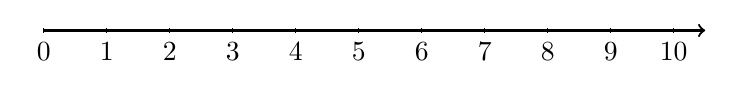
\begin{tikzpicture}[scale=0.8]
            \draw[thick,->] (0,0) -- (10.5,0) node[anchor=north west]{};
            \foreach \x in {0,1,2,3,4,5,6,7,8,9,10} \draw (\x cm,1pt) -- (\x cm,-1pt) node[anchor=north]{$\x$}; 
            \end{tikzpicture}
\end{description}

\subsubsection*{$\mathbb{Z}$ ) Numeri Interi}
        \begin{description}
            \item \textbf{Definizione: } \[\mathbb{Z} = \{\pm 1,\pm 2,\pm 3...\} \longrightarrow \mathbb{N} \subset \mathbb{Z} \enspace {(Naturali = Interi positivi)}\]
            \item \textbf{Rappresentazione decimale: }  \[\mathbb{Z} \owns i = \pm (c_k 10^k + c_{k-1} 10^{k-1} + ... + c_0) \enspace{} {con} \enspace{} c_i \in \{0,1,2,3...,9\}\enspace{} {(cifre)}\]
            \[i = \pm c_k c_{k-1} ... c_0\]
            \item \textbf{Operazioni: } Medesime in $\mathbb{N}$ + \underline{\textbf{Differenza} $a-b$}
            \item \textbf{Proprietà delle op.:}
                \begin{description}
                    \item \textbf{Commutativa} {Non vale per la differenza !}
                    \item \textbf{Associativa} {Per la differenza vige \textit{Regola dei Segni}: } $(a-b) - c = a - (b + c)$
                    \item \textbf{Distributiva} 
                \end{description}
            \item \textbf{Rappresentazione Grafica: }
            \item
            \item 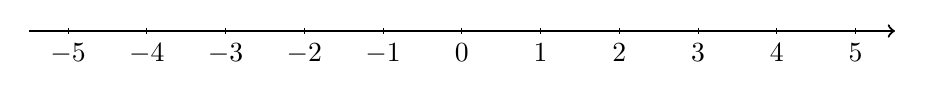
\begin{tikzpicture}
            \draw[thick,->] (-5.5,0) -- (5.5,0) node[anchor=north west]{};
            \foreach \x in {-5,-4,-3,-2,-1,0,1,2,3,4,5} \draw (\x cm,1pt) -- (\x cm,-1pt) node[anchor=north]{$\x$}; 
            \end{tikzpicture}
\end{description}
\subsubsection*{$\mathbb{Q}$ ) Numeri Razionali}
        \begin{description}
            \item \textbf{Definizione: } \[\mathbb{Q} = \{z/n : z \in \mathbb{Z}, n \in \mathbb{N}_+\} \longrightarrow \mathbb{N}, \mathbb{Z} \subset \mathbb{Q} \enspace (n = 1)\]
            \item \textbf{Rappresentazione decimale: }  \[\mathbb{Q} \owns r = c_k 10^k + c_{k-1} 10^{k-1} + ... + c_0 + d_1 10^{-1} + d_2 10^{-2} + ... \enspace{} {con} \enspace{} c_i \in \{0,1,2,3...,9\}\enspace{} {(cifre)}\]
            \[r = c_k c_{k-1} ... c_0 , d_1 d_2 ...\]
            \item \textit{\textbf{Nota:} Le cifre decimali dopo la virgola 
            \begin{itemize}
                \item[(a)] Sono tutte 0 a partire da un certo indice
                \item[(b)] Sono la ripetizione di una sequenza di cifre $\longrightarrow$ numeri periodici (sequenza = \underline{periodo})
            \end{itemize}}
            \item \textbf{Operazioni: } Medesime in $\mathbb{N}$, $\mathbb{Z}$ + \underline{\textbf{Quoziente } $\frac{a}{b}$}
            \item \textbf{Rappresentazione Grafica: }
            \item
            \item 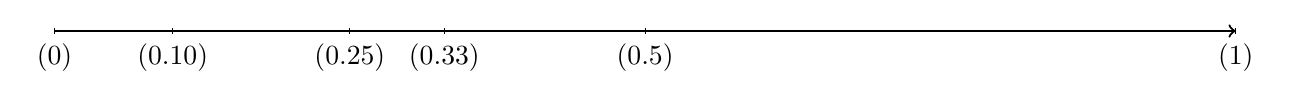
\begin{tikzpicture}
            \draw[thick,->] (0,0) -- (15,0) node[anchor=north west]{};
            \foreach \x in {0,0.10,0.25,0.33,0.5,1} \draw (15*\x cm,1pt) -- (15*\x cm,-1pt) node[anchor=north]{(\x)};
    \end{tikzpicture}
\end{description}
\subsubsection*{Da $\mathbb{Q}$ a $\mathbb{R}$}
Si considera ad esempio il problema dell'\textit{incommensurabilità} tra la diagonale ed il lato del quadrato:
\begin{center}
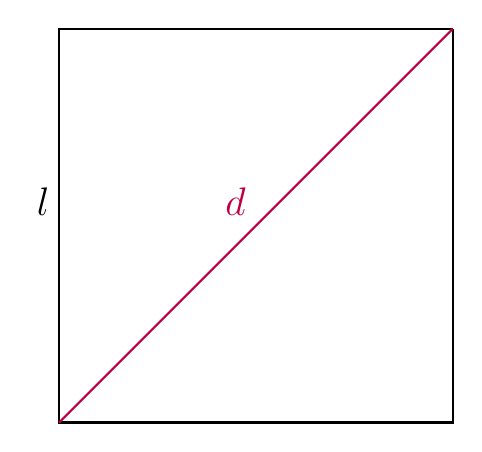
\begin{tikzpicture}
\draw[thick,color=black] (5,5) -- (5,0) -- (0,0) -- (0,5) -- (5,5);
\draw[](0,2.5) node[above left]{\Large $l$};
\draw[thick,color=purple](0,0) -- (5,5) -- (2.5,2.5) node[above left]{\Large $d$};
\end{tikzpicture}
\end{center}
$\mathbb{Q}$ non risulta sufficiente per definire tutti i punti della retta continua (impossibile costruire isomorfismo) $\longrightarrow$ si definisce $\mathbb{R}$

\section{L'insieme dei reali}
\subsection{Ordinamento totale}
\begin{prop}
    Siano $a, b \in \mathbb{R}$. Allora $a \leq b$ $\lor$ $a > b$.
    \\Rispetto alle operazioni algebriche:
    \begin{itemize}[label = $\square$]
        \item $a \leq b, c \in \mathbb{R} \enspace : a + c \leq b + c$
        \item $a \leq b, c \in \mathbb{R}_+ \enspace : c \cdot a \leq c \cdot b$
    \end{itemize}
\end{prop}

\subsection{Valore assoluto}
\begin{defin}
    Sia $a \in \mathbb{R}$. Se ne definisce il valore assoluto secondo:
    \[|a| = \begin{cases}
        a & se \enspace a \geq 0\\
        -a & se \enspace < 0 
    \end{cases}\]
\end{defin}
\subsubsection*{Proprietà}
\begin{enumerate}
    \item \textbf{Positività} $\forall a \in \mathbb{R}$ $|a| \geq 0$; $|a| = 0$ $\Leftrightarrow$ $a = 0$
    \item \textbf{Simmetria} $\forall a,b \in \mathbb{R}$ $|a - b| = |b - a|$
    \item \textbf{Disuguaglianza triangolare} $\forall a,b \in \mathbb{R}$ $|a+b| \leq |a| + |b|$
\end{enumerate}
\textbf{Dimostrazione della triangolare}
\begin{proof}
    Si osserva innanzitutto che $|a \cdot b| = |a| \cdot |b|$ (dimostrazione immediata). Si procede dunque elevando al quadrato i membri della disuguaglianza:
    \[|a+b| \leq |a| + |b| \enspace \Leftrightarrow \enspace |a + b|^2 \leq (|a| + |b|)^2 \enspace ; \enspace a^2 +2ab + b^2 \leq a^2 + b^2 + 2 |a| |b|\]
    Dunque da quanto osservato, semplificando si riconduce a $ab \leq |a||b| \enspace \Rightarrow \enspace ab \leq |ab|$ che è verificata per definizione del v.ass.
\end{proof}

\subsubsection*{Ulteriori proprietà}
\begin{prop}
    \[\forall n \in \mathbb{N}_+ \enspace a_1, ... a_n \in \mathbb{R} :\]
    \begin{enumerate}
        \item 
        \[|a_1 + ... + a_n| \leq |a_1| + ... + |a_n| \enspace \Leftrightarrow \enspace |\sum \limits_{h=1}^n a_h| \leq \sum \limits_{h=1}^n |a_h|\]
        \item
        \[|a_1 \cdot ... \cdot a_n| \leq |a_1| \cdot ... \cdot |a_n| \enspace \Leftrightarrow \enspace |\prod \limits_{h=1}^n a_h| \leq \prod \limits_{h=1}^n |a_h|\]
    \end{enumerate}
\end{prop}

\subsection{Spazio Metrico}
\begin{defin}
    Sia dato un insieme $X$ e una funzione $d : X \times X \rightarrow \mathbb{R}$ che soddisfi:
    \begin{enumerate}
        \item $\forall a,b \in X$ $d(a,b) \geq 0$ $\land$ $d(a,b) = 0 \Leftrightarrow a = b$
        \item $\forall a,b \in X$ $d(a,b) = d(b,a)$
        \item$\forall a,b,c \in X$ $d(a,c) \leq d(a,b) + d(b,c)$
    \end{enumerate}
    $d$ si definisce \textbf{distanza} o \textbf{metrica} su X. La coppia $(X,d)$ è definita \textbf{spazio metrico}.
\end{defin}

\subsection{Intervalli}
\begin{defin}
    Siano $a, b \in \mathbb{R}$. Si definiscono:
    \begin{itemize}[label = $\circ$]
        \item \textbf{Intervallo chiuso} di estremi $a$ e $b$
        \[[a,b] = \{x \in \mathbb{R} : a \leq x \leq b\}\]
        \item \textbf{Intervallo aperto} di estremi $a$ e $b$
        \[]a,b[ = \{x \in \mathbb{R} : a < x < b\}\]
        \item \textbf{Intervallo semiaperto} a destra o sinistra a seconda dell'appartenenza degli estremi ($[a,b[$ oppure $]a,b]$)
        \item \textbf{Altri intervalli} di estremi $a$ o $b$
        \[[a,+\infty[ = \{x \in \mathbb{R} : x \geq a\}\]
        \[[-\infty, b[ = \{x \in \mathbb{R} : x \leq b\}\]
    \end{itemize}
    In generale si definisce intervallo \textbf{un sottoinsieme connesso della retta reale}. \'E possibile dimostrare che le due definizioni sono equivalenti.
\end{defin}
\begin{oss}
    I simboli $\pm \infty$ \underline{non indicano numeri reali}, infatti $\mathbb{R} = ]-\infty, + \infty[$
\end{oss}

\subsubsection{Punti interni ed estremi}
\begin{defin}
    I punti che delimitano un intervallo sono detti \textbf{estremi o punti di frontiera}, gli altri sono \textbf{punti interni}
\end{defin}

\subsection{Insiemi limitati}
\begin{defin}
    Sia $A \subset \mathbb{R}$ diverso dall'insieme vuoto ($A \neq \emptyset$). Si definisce:
    \begin{itemize}
        \item \textbf{Superiormente limitato} se $\exists b \in \mathbb{R}$ : $x \leq b$ $\forall x \in A$. Un qualsiasi $b$ che realizzi la proprietà enunciata è definito \textbf{maggiorante} di $A$
        \item \textbf{Inferiormente limitato} se $\exists a \in \mathbb{R}$ : $x \geq a$ $\forall x \in A$. Un qualsiasi $a$ che realizzi la proprietà enunciata è definito \textbf{minorante} di $A$
        \item \textbf{Limitato} se $\exists r \in \mathbb{R}$ : $|x| \leq r$ $\forall x \in A$
    \end{itemize}
\end{defin}

\subsubsection{Massimi e minimi}
\begin{defin}
    $A \subset \mathbb{R}$ ammette massimo se $\exists x_M \in A$ : $\forall x \in A$ $x \leq x_M$
    \\$x_M$ è definito massimo di $A$ e si indica $x_M = \max A$
    \\$A \subset \mathbb{R}$ ammette minimo se $\exists x_m \in A$ : $\forall x \in A$ $x \geq x_m$
    \\$x_m$ è definito minimo di $A$ e si indica $x_m = \min A$
\end{defin}
\begin{oss}
    \begin{enumerate}
        \item Massimo e minimo di un insieme, se esistono, sono unici
        \item Se un insieme ammette massimo, allora \textbf{è superiormente limitato}. Analogamente per il minimo. Si noti che \textbf{non è valida l'implicazione contraria!}
    \end{enumerate}
\end{oss}

\subsubsection{Estremi sup e inf}
\begin{defin}
    Sia $A \subset \mathbb{R}$ superiormente limitato. L'estremo superiore di $A$ è \textbf{il minimo dei maggioranti} di A. Si indica con $\sup A$.
     Sia invece $B \subset \mathbb{R}$ inferiormente limitato. L'estremo inferiore di $B$ è \textbf{il massimo dei minoranti} di $B$. Si indica con $\inf B$.
\end{defin}
\begin{oss}
    \begin{enumerate}
        \item Ciascun estremo è definito da due proprietà: \textbf{a)} \'E un minorante / maggiorante e \textbf{b)} \'E il massimo / minimo m.
    \item Gli estremi di un intervallo, se esistono, sono unici (si dimostra analogamente a massimo e minimo).
    \item Se un insieme ammette massimo, tale massimo coincide con l'estremo superiore; analogamente se ammette minimo con l'estr. inferiore ($\exists \max A \implies \max A = \sup A$; $\exists \min A \implies \min A = \inf A$)
    \end{enumerate}
\end{oss}

\begin{defin}
    Se $A \subset \mathbb{R}$ superiormente illimitato $\sup A = + \infty$ (analogamente per inf. con $- \infty$)
\end{defin}
\textbf{Nota: } Per $\emptyset$ $\inf \emptyset = + \infty$; $\sup \emptyset = - \infty$

\subsection{Completezza di \texorpdfstring{$\mathbb{R}$}{$\mathbb{R}$}}
\begin{ass}
Sia $A \subset \mathbb{R}$ superiormente limitato. Allora A ammette un estremo superiore.
\[A \subset \mathbb{R} : \enspace \exists b \in \mathbb{R}: x \leq b \enspace \forall x \in A \Longrightarrow \exists \sup A\]
\'E possibile riformulare analogamente per inferiormente limitato.
\end{ass}
\textbf{Applicazione: } $\mathbb{Q}$ non è completo: si verifica per l'irrazionalità della radice di 2. Si dimostra invece che $x^2 = 2$ ha soluzione positiva in $\mathbb{R}$:
\begin{proof}
    Si definisce $A = \{x \in \mathbb{Q} : x^2 < 2\}$. $A \subset \mathbb{R}$ in quanto $\mathbb{Q} \subset \mathbb{R}$ e superiormente limitato. Dunque per l'assioma di completezza $\exists \sup A =: s$ $\implies s \in \mathbb{R}$. Si può verificare che non può essere nè $s^2 < 2$ nè $s^2 > 2$.
\end{proof}

\subsection{Assioma di Dedekind}
Rappresenta una formulazione equivalente a quella vista dell'assioma di completezza:
\begin{ass}
    Siano $A, B \neq \emptyset$ sottoinsiemi di $\mathbb{R}$ tali per cui 
    \[\forall a \in A \enspace, \enspace b \in B \enspace a \leq b\]
    Allora
    \[\forall a \in A\enspace, \enspace b \in B \quad \exists c \in \mathbb{R} \enspace : \enspace a \leq c \leq b\]
\end{ass}

\paragraph{Esistenza della radice n-esima di un numero reale}
    Siano $n \in \mathbb{N}_+$, $a \in \mathbb{R}$. Si consideri l'equazione $x^n = a$. Si esclude il caso triviale $n = 1$. Si ha:
    \begin{itemize}
        \item per $n$ dispari l'equazione ammette un'unica radice in $\mathbb{R}$ e si ha $x = a^{\frac{1}{n}} = \sqrt[n]{a}$.
        \item per $n$ pari si ha:
        \begin{enumerate}
            \item $\forall a > 0$ l'equazione ha due soluzioni di medesimo valore ass. e segno opposto
            \item per $a = 0$ una sola soluzione $x = 0$
            \item per $\forall a < 0$ nessuna soluzione reale
        \end{enumerate}
    \end{itemize}

\section{Elementi di Combinatoria}
\paragraph{Permutazioni} $P_n = n!$
\paragraph{Disposizioni} senza ripetizione: $D_{n, k} = \frac{n!}{(n-k)!}$ || con ripetizione: $D_{n, k}^* = n^k$
\paragraph{Combinazioni} senza ripetizione: $C_{n, k} = \binom{n}{k} = \frac{n!}{k! (n-k)!}$ || con ripetizione: $C_{n, k}^* = \binom{n + k - 1}{k} = \frac{(n+k-1)!}{k! (n-1)!}$

\subsection{Binomio di Newton}
\begin{prop}
    Siano $a, b \in \mathbb{R}$ e $n \in \mathbb{N}$. Allora 
    \[(a+b)^n = \sum \limits_{h = 0}^n \binom{n}{h} a^{n - h} b^h\]
\end{prop}
\begin{proof}
    \'E possibile dedurre la formula considerando, per ciascuna coppia di esponenti, le possibili scelte nel prodotto tra $n$ binomi $a+b$. Si dimostra dunque la validità per ogni valore di $n$ per induzione:
    \begin{itemize}
        \item Per $n_0 = 0$ la dim. è triviale: 
        \[\sum \limits_{h = 0}^n \binom{0}{h} a^{0 - h} b^h = \binom{0}{0} a^0 b^0 = 1 = (a+b)^0\]
        \item Si assuma l'ipotesi induttiva per $n$, e si dimostri l'implicazione della validità della proposizione per $n+1$:
        \[(a+b)^{n+1} = (a+b) \cdot (a+b)^n = (a+b) \cdot \sum \limits_{h = 0}^n \binom{n}{h} a^{n - h} b^h = \sum \limits_{h = 0}^n \binom{n}{h} a^{n + 1 - h} b^h + \sum \limits_{h = 0}^n \binom{n}{h} a^{n - h} b^{h + 1}\]
        Si isola dalla prima sommatoria il termine per $h = 0$ e dalla seconda per $h = n$:
        \[(a+b)^{n+1} = a^{n+1} + \sum \limits_{h = 1}^n \binom{n}{h} a^{n + 1 - h} b^h + \sum \limits_{h = 0}^{n-1} \binom{n}{h} a^{n - h} b^{h +1} + b^{n+1}\]
        Si effettua un cambiamento dell'indice di somma della seconda sommatoria: $l = h+1$ $\implies$ $h = l-1$:
        \[\sum \limits_{h = 0}^{n-1} \binom{n}{h} a^{n - h} b^{h +1} = \sum \limits_{l = 1}^{n} \binom{n}{l -1} a^{n + 1 - l} b^{l}\]
        Indicando anche l'indice della prima sommatoria con $l$ è ora possibile raccogliere in un'unica s.:
        \[\sum \limits_{l = 1}^n \binom{n}{h} a^{n + 1 - l} b^l +  \sum \limits_{l = 1}^{n} \binom{n}{l -1} a^{n + 1 - l} b^{l} =  \sum \limits_{l = 1}^{n} (\binom{n}{l -1} + \binom{n}{l}) a^{n + 1 - l} b^{l}\]
        Si ha
        \[ \sum \limits_{l = 1}^{n} \binom{n}{l -1} a^{n + 1 - l} b^{l} = \frac{n!}{(n-l)! l!} + \frac{n!}{(n-j+1)! (j-1)!} = \frac{n!}{(n-j)! (j-1)!} \bigg( \frac{1}{l} + \frac{1}{n-l+1}\bigg) = \]
    \[= \frac{n!}{(n-j)! (l-1)!} \bigg( \frac{n+1 \cancel{-l} \cancel{+l}}{l (n-l+1)} \bigg) = \frac{(n+1)!}{l! (n+1-l)!} = \binom{n+1}{l}\]
    Dunque
    \[(a+b)^{n+1} = \binom{n+1}{0} a^{n+1} + \sum \limits_{l = 1}^n \binom{n+1}{l} a^{n + 1 - l} b^l + \binom{n+1}{n+1} b^{n+1} = \sum \limits_{l = 0}^{n+1} \binom{n+1}{l} a^{n + 1 - l} b^l\]
    \end{itemize}
\end{proof}

\section{Complementi di insiemistica}

\subsection{Prodotto Cartesiano}
\begin{defin}
Siano $X,Y \neq \emptyset $. Si definisce prodotto cartesiano di X e Y l'insieme di tutte le possibili coppie \underline{ordinate} di elementi di $X$ e di $Y$.
\[X \times Y = \{ (x,y) : x \in X, \enspace y \in Y\}\]
\end{defin}
\textbf{Nota 1} Il prodotto cartesiano \underline{non è commutativo}, salvo il caso in cui $X = Y$. Allora è possibile scrivere: \[X \times X = X^2\]
\textbf{Nota 2} Un particolare sottoinsieme di tale p.c. è la \underline{diagonale}: 
\[X \times X \supset \Delta = \{ (x,x) : x \in X\}\]
\textbf{Nota 3} E' possibile iterare il prodotto; ad esempio da  $\mathbb{R}$:
\[\mathbb{R} \times \mathbb{R} = \mathbb{R}^2 = \{(x,y) : x, y \in \mathbb{R}\}\]
\[\mathbb{R} \times \mathbb{R} \times \mathbb{R}= \mathbb{R}^3 = \{(x,y,z) : x, y, z \in \mathbb{R}\}\]

\subsection{Relazioni nel Piano}
\begin{defin}
Una relazione è un sottoinsieme del piano, ovvero $R \subset \mathbb{R}^2$. Un reale $x$ si dice \textbf{in relazione ad un altro reale y attraverso $R$} se $(x,y) \in R$.
\end{defin}

\subsubsection{R. di equivalenza}
\begin{defin}
Una relazione di equivalenza è una relazione $\mathcal{R}(x,y)$ che soddisfa le seguenti proprietà:
\begin{enumerate}
    \item \textbf{Simmetrica} $x\mathcal{R}y \enspace \implies y\mathcal{R}x$
    \item \textbf{Riflessiva} $\forall x \enspace x\mathcal{R}x$
    \item \textbf{Transitiva} $x\mathcal{R}y \enspace \land \enspace y\mathcal{R}z\enspace \implies \enspace x\mathcal{R}z$
\end{enumerate}
Per la notazione: $x\mathcal{R}y$ = '$x$ è equivalente a $y$ rispetto alla relazione $\mathcal{R}$.
\end{defin}

\paragraph{Classi di eq. e insieme quoziente}
\begin{defin}
    Dato un elemento $x$ si definisce classe di equivalenza di $x$ rispetto alla relazione $\mathcal{R}$ l'insieme costituito da tutti gli elementi equivalenti ad $x$ rispetto alla relazione:
    \[[x] = \{y \in \mathbb{R} : y\mathcal{R}x\}\]
    $x$ si definisce \textbf{rappresentante} della classe.
\end{defin}
\'E intuitivo verificare che due classi di equivalenza coincidono oppure sono disgiunte (sufficiente applicare transitività). Dunque una rel. d'eq. determina una \textbf{partizione} dell'insieme considerato (in questo caso, la retta reale).
\begin{defin}
    L'insieme di tutte le classi di equivalenza in un insieme $X$ rispetto ad una data relazione $\mathcal{R}$ si definisce \textbf{insieme quoziente} e si indica:
    \[X / \mathcal{R}\]
\end{defin}

\subsection{Funzioni e Cardinalità}
\begin{defin}
    Si definisce cardinalità di un insieme il numero dei suoi elementi. Se $A$ ha cardinalità $n$ si indica con $\# A = n$.
\end{defin}
\begin{prop}
    Siano $X$, $Y$ insiemi (non necessariamente finiti). Allora:
    \begin{itemize}[label = $\square$]
        \item $\#X \leq \#Y$ se $\exists f : X \xrightarrow[]{1-1} Y$ (ovvero è possibile definire una funzione iniettiva da $X$ a $Y$)
        \item $\#X \geq \#Y$ se $\exists f : X \xrightarrow[]{su} Y$ (suriettiva)
        \item $\#X = \#Y$ se $\exists f : X \xrightarrow[su]{1-1} Y$ (una biezione / isomorfismo)
    \end{itemize}
\end{prop}

\subsection{Cardinalità di insiemi infiniti}
L'insieme $\mathbb{N}$ è un insieme infinito numerabile, definito dagli assiomi di Peano:
\begin{defin}
    Il sistema dei numeri naturali è costituito da un insieme $\mathbb{N}$ in cui è definita un'applicazione $\sigma : \mathbb{N} \rightarrow \mathbb{N}$ che soddisfi:
    \begin{itemize}
        \item $\exists 1 \in \mathbb{N} : 1 \notin \sigma (\mathbb{N})$
        \item $\sigma$ è iniettiva
        \item Se $\mathcal{A} \subset \mathbb{N}$, $1 \in \mathcal{A}$ e $\sigma(\mathcal{A}) \subset \mathcal{A}$ allora $\mathcal{A} = \mathbb{N}$
    \end{itemize}
    Il terzo assioma corrisponde al principio di induzione.
\end{defin}
\subsubsection*{Insiemi numerabili}
\begin{defin}
    Un insieme è numerabile se è possibile costruire una biezione da esso a $\mathbb{N}$, ovvero possono essere posti in corrispondenza biunivoca.
    \\La cardinalità di $\mathbb{N}$ è definita $\aleph_0$
\end{defin}
\textbf{Nota: } l'insieme dei numeri pari e quello dei dispari sono contenuti propriamente in $\mathbb{N}$ ma hanno la medesima cardinalità in quanto è possibile costruire una biezione. In generale per insiemi infiniti è possibile adottare la seguente definizione:

\begin{defin}
    Un insieme si dice infinito se \textbf{è possibile costruire una biezione con un suo sottoinsieme proprio}. In caso contrario si dice finito
\end{defin}
In forma di teorema:
\begin{ther}
    Un insieme $A$ ha cardinalità infinita \textbf{se e solo se} $\exists B \subsetneq A$ : $\#B = \#A$
\end{ther}
\begin{proof}
    $\mathbf{\implies)}$ Si dimostra che se $\#A = \infty$ si ha $\#A \geq \#\mathbb{N}$. 
    \\Sia un qualsiasi elemento $a_1 \in A$. Si consideri quindi un altro elemento $a_2 \in A \setminus \{a_1\}$ e si iteri fino ad un qualsiasi $a_n \in A \setminus \{a_1, a_2, ..., a_{n-1}\}$ (essendo $A$ infinito con cardinalità maggiore o uguale a quella dei naturali, è possibile farlo per qualsiasi $n$)
    \\Si definisca quindi una funzione $f: \mathbb{N}_+ \xrightarrow[]{1-1} A$ secondo $f(n) = a_n$. Essendo $A$ infinito è possibile definirla e quindi si ha $\#A \geq \#\mathbb{N}_+$. Ma essendo l'insieme dei naturali non nulli di cardinalità uguale a quella di $\mathbb{N}$ (sufficiente costruire la biezione $f(n) = n+1$) si ha la dimostrazione.
    \\Si considerino i casi possibili. Per $\#A = \#\mathbb{N}$ si identifichi $A$ con $\mathbb{N}$\'E sufficiente definire $B$ secondo $B := f(\{numeri \enspace pari\}) \subsetneq A$. Per $\#A > \#\mathbb{N}$ si consideri una partizione di $A$: $A = A_1 \cup A_2$ $\land$ $A_1 \cap A_2 = \emptyset$ tale per cui sia possibile porre in biezione $A_1$ e $\mathbb{N}$. Si procede quindi analogamente alla trattazione per l'altro caso ottenendo un sottoinsieme proprio di $A_1$, sia $B_1$, che verifica $\#B_1 = \#A_1$. \'E quindi sufficiente definire $B = B_1 \cup A_2$.
    \\$\mathbf{\Leftarrow)}$ L'implicazione inversa è dimostrata per assurdo: se $B$ contenuto propriamente in $A$ e si assume $\#A < \infty$, sia $\#A = n$ $\implies$ $\#B \leq n-1$. Dunque è impossibile costruire una funzione iniettiva da $A$ a $B$, il che contraddice l'ipotesi di uguale cardinalità.
\end{proof}
Dalla numerabilità di $\mathbb{N}$ consegue quella di $\mathbb{Z}$ e $\mathbb{Q}$. Per unioni di un numero non finito di insiemi numerabili vale il seguente teorema:
\begin{ther}
    L'unione di un'infinità numerabile di insiemi numerabili è numerabile.
\end{ther}
Ciò non vale per l'insieme dei numeri reali, che è non numerabile secondo quanto dimostrato dall'argomento diagonale di Cantor.
\begin{proof}
    Si considera l'intervallo $]0,1[ \subset \mathbb{R}$. \'E sufficiente dimostrare che la sua cardinalità sia strettamente maggiore di quella di $\mathbb{N}$.
    \\Si consideri la rappresentazione decimale dei numeri reali compresi nell'intervallo. Se fosse numerabile, sarebbe possibile posizionare tutte le cifre di tali numeri in una tabella nel modo seguente:
    \[\begin{matrix}
    0. & a_{11} & a_{12} & \cdots \\
    0. & a_{21} & a_{22} & \cdots \\
    \vdots & \ddots & \ddots & \ddots \\
    0. & a_{n1} & a_{n2} & \cdots \\
    \vdots & \ddots & \ddots & \ddots
    \end{matrix}\]
    Si consideri quindi il numero reale $0.c_1 c_2 \cdots$ definito secondo $c_i \neq a_ii$ (ovvero ogni cifra diversa dall'elemento di medesimo indice sulla diagonale della tabella costruita). Tale numero, per costruzione, non appartiene alla tabella ma appartiene all'intervallo considerato. Si è dunque verificata la tesi: non è possibile costruire una funzione iniettiva dall'intervallo ai naturali, dunque la cardinalità del primo è strettamente maggiore e di conseguenza quella dell'insieme $\mathbb{R}$.
\end{proof}
\textbf{Nota sulla dim: } la dimostrazione non tiene conto della non unicità di rappresentazione decimale ($0.4 = 0.3\overline{9}$) ma è possibile porre rimedio e mantenere la validità dell'argomento.


\section{Funzioni}
\begin{defin}
Siano $X$ e $Y$ due insiemi. Una funzione $f$ definita in $X$ a valori in $Y$ è una corrispondenza che associa ad ogni elemento di $X$ \underline{al più un elemento} di $Y$
\[y = f(x)\]
L'insieme di partenza è definito \textbf{dominio} della funzione e quello di arrivo \textbf{codominio}. L'insieme di tutti gli elementi del codominio mappati da $f$ è definito \textbf{immagine} della funzione.
\[X = dom f \quad im f = f(X)\]
L'insieme degli elementi del prodotto cartesiano tra dominio e codominio il cui secondo ingresso è immagine del primo attraverso la funzione è definito \textbf{grafico} di $f$.
\[\mathbb{R}^2 \supset \Gamma (f) = \{(x,y) \in \mathbb{R}^2 \enspace : \enspace y = f(x) \}\]
Dato un elemento del codominio, la corrispondente \textbf{controimmagine} attraverso la funzione è l'insieme degli elementi del dominio mappati nel suddetto el. del codom. dalla funzione. Se l'elemento non appartiene all'immagine, la sua controimmagine è l'insieme vuoto. \'E possibile anche definire la controimm. di un sottoinsieme del codominio.
\[f^{-1}(y) = \{x \in X \enspace : \enspace f(x) = y\}\] \[B \subset Y \enspace \implies \enspace f^{-1}(B) = \{x \in X \enspace : \enspace f(x) \in B\}\]
\end{defin}
\subsubsection{Estremi di una funzione}
\begin{defin}
Data $f :  A \subseteq \mathbb{R} \rightarrow \mathbb{R}$ Si definiscono \textbf{estremo superiore} e \textbf{inferiore di f}, rispettivamente, l'estremo superiore e inferiore dell'immagine, qualora questa ne ammetta nei reali.
\[\sup \limits_{x \in A} f(x) \enspace = \enspace \sup f(A)\]
\[\inf \limits_{x \in A} f(x) \enspace = \enspace \inf f(A)\]
Dunque $f$ si definisce \textbf{superiormente limitata su A} se l'immagine di $A$ ammette estremo superiore, analogamente se inf. limitata. Se $\sup f(A) \in f(A)$ e/o $\inf f(A) \in f(A)$, ovvero l'estremo superiore e/o inferiore appartiene all'immagine, allora $f$ ammette massimo e/o minimo.
\end{defin}
\subsection{Suriettività, iniettività, biettività, funzione inversa}
\subsubsection{F. suriettiva}
\begin{defin}
Una funzione si dice \textbf{suriettiva (su)} se la sua immagine coincide con il codominio. Data $f : X \subseteq \mathbb{R} \rightarrow Y \subseteq \mathbb{R}$:
\[im f = Y\]
\end{defin}
\subsubsection{Iniettiva}
\begin{defin}
Una f. si dice \textbf{iniettiva (1-1)} se a ciascun elemento del codominio è associata al più una controimmagine, ovvero se la funzione mappa in un elemento dell'immagine un solo el. del dominio.
\\Alternativamente, se $f(x_1) = f(x_2) \enspace \implies \enspace x_1 = x_2$
\end{defin}

\subsubsection{Funzioni invertibili}
\begin{prop}
Se una funzione è iniettiva, è possibile \textbf{invertirla}. Ovvero è possibile costruire una funzione che mappi ogni elemento del codominio in un solo elemento del dominio. Ciò corrisponde al fatto che \textbf{la controimmagine} attraverso la funzione \textbf{è una funzione}, ovvero una corrispondenza univoca.
\end{prop}
\begin{oss}
Si noti che se l'inversa è una corrispondenza univoca e lo è anche la funzione, l'inversa è iniettiva e dunque invertibile; la sua inversa sarà infatti la funzione di partenza.
\end{oss}
Definendo la funzione identità $id_X : X \rightarrow X$ con $id_X (x) = x$ $\forall x \in X$ si ha
\[f^{-1} \circ f = id_{dom f} \enspace f \circ f^{-1} = id_{im f}\]

\subsection{Funzioni elementari: pari e dispari}
\begin{defin}
    Sia $f : \mathbb{R} \rightarrow \mathbb{R}$ (dominio = tutta la retta). Si definisce:
    \begin{itemize}[label = $\square$]
        \item \textbf{pari} se $f(-x) = f(x)$ $\forall x \in \mathbb{R}$
        \item \textbf{Dispari} se $f(-x) = - f(x)$ $\forall x \in \mathbb{R}$
    \end{itemize}
    Una funzione pari è simmetrica rispetto all'asse delle ordinate, una dispari rispetto all'origine.
\end{defin}
Si verifica intuitivamente che per $f$ dispari $f(0) = - f(-0) = - f(0) = 0$

\subsection{F. periodiche}
\begin{defin}
    Una funzione $f : \mathbb{R} \rightarrow \mathbb{R}$ si definisce periodica di periodo $T$ se $\forall x \in \mathbb{R}$ $f(x+T) = f(x)$
    \end{defin}
    Una funzione periodica di periodo $T$ lo è anche di periodo $nT$ $\forall n \in \mathbb{N}_+$

\subsection{Funzioni crescenti, decrescenti, monotòne}
\begin{prop}
Se una funzione $f$ è strettamente monotona (crescente o decrescente), allora è iniettiva.
\end{prop}
\begin{proof}
Si procede per assurdo, negando la tesi. Sia dunque $f$ non iniettiva, ovvero $\exists x_1, x_2 \in domf, x_1 \neq x_2 \enspace : \enspace f(x_1) = f(x_2)$. Per l'ordinamento totale dei reali, si deve avere $x_1 > x_2$ o $x_1 < x_2$. Ma ciò comporta che la funzione assuma un valore uguale su due punti del dominio di cui uno è maggiore (o minore) dell'altro. Ciò contraddice l'ipotesi per cui è monotòna crescente o decrescente: si ha quindi l'assurdo, e la tesi è dimostrata.
\end{proof}

\subsection{F. Trigonometriche}
\paragraph{Addizione e sottrazione, duplicazione, prostaferesi}
Si riportano le formule relative per le trigonometriche (seno e coseno):
\textbf{Addizione / Sottrazione}
\[\cos(\alpha - \beta) = \cos \alpha \cos \beta + \sin \alpha \sin \beta \enspace | \enspace \cos(\alpha + \beta) = \cos \alpha \cos \beta - \sin \alpha \sin \beta\]
\[\sin(\alpha - \beta) = \sin \alpha \cos \beta - \cos \alpha \sin \beta \enspace | \enspace \sin(\alpha + \beta) = \sin \alpha \cos \beta + \cos \alpha \sin \beta\]
\textbf{Duplicazione}
\[\sin (2\alpha) = 2 \sin \alpha \cos \alpha \quad \bigg| \quad \cos (2\alpha) = \cos^2\alpha - \sin^2 \alpha\]
\textbf{Prostaferesi}
\[\cos \alpha - \cos \beta = -2 \sin \big(\frac{\alpha - \beta}{2}\big)\sin\big(\frac{\alpha + \beta}{2}\big)\]
\[\sin \alpha - \sin \beta = 2 \sin \big(\frac{\alpha - \beta}{2}\big)\cos\big(\frac{\alpha + \beta}{2}\big)\]

\subsection{Coordinate polari piane}
Le coordinate di un punto possono essere definite da una coppia $(r, \theta)$ in cui:
\begin{itemize}
    \item $r$ indica la distanza dall'origine
    \item $\theta$ (definito in radianti) l'angolo formato dalla retta passante per l'origine ed il punto rispetto alle ascisse (definito a meno di multipli di $2\pi$)
\end{itemize}
Per passare dalle cartesiane alle polari e viceversa:
\[r = \sqrt{x^2 + y^2} \enspace \theta = \arctan\bigg( \frac{y}{x} \bigg) \quad \bigg| \quad x = r \cos \theta \enspace y = r \sin \theta\]

\section{Numeri complessi}
$z = x + iy$
\begin{itemize}
    \item Coniugato $\overline{z} = Re (z) - Im (z) = a -ib$
    \item Proprietà del coniugio $\overline{z_1 + z_2} = \overline{z_1} + \overline{z_2}$; $\overline{z_1 \cdot z_2} = \overline{z_1} \cdot \overline{z_2}$; $\overline{\frac{1}{z}} = \frac{1}{\overline{z}}$ per $z \neq 0$. Se $z_1, z_2 \neq 0$ inoltre $\overline{\frac{z_1}{z_2}} = \frac{\overline{z_1}}{\overline{z_2}}$
    \item Modulo $|z| = \sqrt{a^2 + b^2} = \sqrt{z \cdot \overline{z}}$
    \item Inverso $z^{-1} = \frac{\overline{z}}{|z|^2}$ $\implies$ $z \cdot z^{-1} = z^{-1} \cdot z = 1$
    \item Parte reale e immaginaria $Re(z) = (z + \overline{z}) / 2$ , $Im (z) = (z - \overline{z}) / 2i$
    \item Forma trigonometrica $z = x + iy = r (\cos \theta + i \sin \theta)$ con $|z| = r$, $\theta$ univocamente determinato imponendo $\theta \in [0, 2\pi[$
    \begin{itemize}[label = $\ast$]
        \item Addizione $z_1 \cdot z_2 = r_1 r_2 (\cos{\theta_1 + \theta_2} + i \sin{\theta_1 + \theta_2})$
    \end{itemize}
    \item Forma esponenziale $e^{i \theta} = \cos \theta + i \sin \theta$ $\implies$ $z = r e^{i\theta}$. Per il prodotto $z_1 \cdot z_2 = r_1 r_2 e^{i (\theta_1 + \theta_2)}$
    \item Radice $n$-esima $z^n = r^n e^{i n\theta} = w$. Espresso $w = \rho e^{i \phi}$ si ha:
    \[\begin{cases}
        r = \sqrt[n]{\rho} \\
        \theta = \frac{\phi + 2 k \pi}{n} & \textrm{con $k \in \mathbb{Z}$ e $k = 0, 1, ..., n-1$}
    \end{cases}\]
    L'equazione ha quindi $n$ soluzioni distinte: corrispondono ai vertici di un poligono regolare.
\end{itemize}

\section{Successioni}
\subsection{Definizione}
\begin{defin}
Una successione è una funzione definita sull'insieme $\mathbb{N}$ dei numeri naturali a valori in $\mathbb{R}$. Il dominio di una successione è superiormente illimitato e può ammettere un punto di minimo $n_0 \in \mathbb{N}$ maggiore di 0. Una successione $a : \mathbb{N} \rightarrow \mathbb{R}$ si indica con $a_n$.
\end{defin}

\subsection{Limiti di successioni}
\subsubsection{Intorni}
\begin{defin}
    Si consideri un punto sulla retta reale $x_0 \in \mathbb{R}$ e un numero reale positivo $r > 0$. Si definisce \textbf{intorno di $x_0$ di raggio $r$} 
    \[I_r(x_0) = ]x_0 - r, x_0 +r[ = \{x \in \mathbb{R} : |x - x_0| < r\}\]
\end{defin}
\begin{oss}
    Se $x_1, x_2 \in \mathbb{R}$ e $x_1 \neq x_2$ allora 
    \[\exists r_1, r_2 > 0 \enspace : \enspace I_{r_1}(x_1) \cap I_{r_2}(x_2) = \emptyset\]
\end{oss}

\begin{defin}
    Si definisce intorno di $+\infty$ di estremo inferiore $a$, con $a \geq 0$: $I_a(+\infty) = ]a, +\infty[$
    \\Analogamente per $-\infty$ con estremo sup. $-a$:
    $I_{a}(-\infty) = ]-\infty, -a[$
\end{defin}

Una data proprietà $p(x)$ \textbf{vale nell'intorno di un punto $c$} se \textbf{esiste un intorno di $c$ tale per cui sia verificata per ogni punto al suo interno}, ovvero $\exists r>0 \enspace : \enspace p(x) \forall x \in I_r(c)$

\subsubsection{Definizione}
\begin{defin}
    Sia data una successione ($n \rightarrow a_n$) e un numero reale $l \in \mathbb{R}$. Allora si definisce:
    \[\lim \limits_{n \rightarrow + \infty} a_n = l \enspace \Leftrightarrow \enspace a_n \xrightarrow[n \rightarrow + \infty]{} l \enspace \Leftrightarrow \enspace \forall \varepsilon > 0 \enspace \exists n_\varepsilon \enspace : \enspace \forall n > n_\varepsilon \enspace |a_n - l| < \varepsilon\]
\end{defin}
In caso di successione convergente, per verificare la correttezza del limite secondo la definizione è necessario verificare che sia possibile determinare il valore limite dell'indice $n_\varepsilon$ per arbitrari valori di $\varepsilon$.

\begin{defin}
    Una successione si definisce convergente se ha limite finito
\end{defin}

\subsubsection{Successioni divergenti}
\begin{defin}
    Una successione $a_n$ tende (o diverge) a $+\infty$, ovverlo $\lim \limits_{n \rightarrow +\infty} a_n = + \infty$ se 
    \[\forall A > 0 \enspace \exists n_A > 0 \enspace : \enspace \forall n> n_A \enspace a_n > A\]
    Analogamente per la divergenza a $-\infty$ con $a_n < -A$
\end{defin}
\textbf{Nota bene: } possono esistere successioni nè convergenti nè divergenti, ovvero limitate ma 'oscillanti' (non monotone). Nel caso di successioni monotone vale invece il seguente teorema:

\subsubsection{Monotone e limiti}
\begin{ther}
    Sia $a_n$ una successione monotona. Allora:
    \begin{enumerate}
        \item $a_n$ è convergente o divergente
        \item se $a_n$ è limitata allora è convergente
    \end{enumerate}
\end{ther}
\begin{proof}
    Si supponga $a_n$ crescente (la trattazione è analoga nel caso di monotona decrescente). Per definizione $a_{n+1} > a_n \enspace \forall n$. 
    \\Se non fosse superiormente limitata, non ammetterebbe maggioranti reali; dunque $\forall A > 0$ $\exists n_A \in \mathbb{N}$ : $a_{n_A} > A$. Essendo crescente, la condizione è verificata $\forall n > n_A$, il che equivale per definizione a $\lim \limits_{n \rightarrow +\infty} a_n = +\infty$, ovvero è divergente.
    \\Se limitata, per l'assioma di completezza ammette almeno un maggiorante (l'estremo superiore). Dunque $\exists L = \sup a_n$. Sia $\varepsilon > 0$; dalla definizione di estr. sup. $\exists n_\varepsilon \in \mathbb{N}$ : $L - \varepsilon < a_{n_\varepsilon}$ in quanto se, per assurdo, non esistesse tale valore della succ., si contraddirebbe la definizione di estremo superiore (minimo dei maggioranti). Poiché monotona crescente, $l - \varepsilon < a_n$ $\forall n > n_\varepsilon$. Essendo $\varepsilon$ positivo, $l + \varepsilon > l$ $\implies$ $|a_n - l| < \varepsilon$ $\forall n > n_\varepsilon$, ovvero per definizione $a_n$ converge all'estremo superiore. Nel caso di monotona decrescente inferiormente limitata il risultato è analogo per l'estremo inferiore.
\end{proof}

\paragraph*{Il numero di Nepero}
\[a_n = \bigg(1 + \frac{1}{n}\bigg)^n\]
Si dimostra che è crescente, limitata e ha limite non razionale.

\paragraph*{Generalizzazione}
\begin{prop}
    Sia $a_n$ successione a valori in $\mathbb{N}$ divergente a $+\infty$. Allora
    \[\bigg(1 + \frac{1}{a_n}\bigg)^{a_n} \longrightarrow e\]
\end{prop}
\begin{proof}
    Si dà per dimostrato il caso $a_n = n$.
    \\Si fissi $\varepsilon > 0$. Per definizione di limite \[\exists n_1 \enspace : \enspace \forall n > n_1 \quad \bigg| \bigg(1 + \frac{1}{n}\bigg)^n - e\bigg| < \varepsilon\]
    Poiché $n_1$ naturale fissato, essendo $a_n$ divergente $\exists n_2$ t.c. $\forall n > n_2$ $a_n > n_1$. Perciò consegue che, assumendo $a_n$ valori naturali ed essendo strettamente crescente e divergente ad infinito, è verificata:
    \[\exists n_2 \enspace : \enspace \forall n > n_1 \quad \bigg| \bigg(1 + \frac{1}{a_n}\bigg)^{a_n} - e\bigg| < \varepsilon\]
    ovvero per definizione la successione considerata tende a $e$.
\end{proof}

\'E possibile un'ulteriore generalizzazione, previa la dimostrazione della seguente:

\begin{prop}
    Data una successione a valori reali, essa diverge a $+\infty$ \textbf{se e solo se} fa altrettanto la sua parte intera. Ovvero
    \[\mathbb{R} \owns a_n \rightarrow +\infty \enspace \Leftrightarrow \enspace [a_n] \rightarrow +\infty\]
\end{prop}
\textbf{Nota sull'enunciato: } La parte intera è definita come \textbf{il più grande intero} $\leq a_n$.
\begin{proof}
    Per definizione di parte intera, $[a_n] \leq a_n < [a_n] + 1$. Applicando il confronto si dimostra: l'implicazione $\implies$ dalla disuguaglianza di destra, quella $\Leftarrow$ dalla dis. di sinistra.
\end{proof}
\begin{prop}
    Sia $a_n$ successione divergente a $+\infty$. Allora
    \[\bigg(1 + \frac{1}{a_n}\bigg)^{a_n} \longrightarrow e\]
    \[\bigg(1 - \frac{1}{a_n}\bigg)^{-a_n} \longrightarrow e\]
    Inoltre, dal secondo risultato: data $b_n \rightarrow - \infty$:
     \[\bigg(1 + \frac{1}{b_n}\bigg)^{b_n} \longrightarrow e\]
\end{prop}
\begin{proof}
    Si applica il confronto:
    \[\bigg(1 + \frac{1}{[a_n]+1}\bigg)^{[a_n]} \leq \bigg(1 + \frac{1}{a_n}\bigg)^{a_n} \leq \bigg(1 + \frac{1}{[a_n]}\bigg)^{[a_n]+1}\]
    Studiando il primo membro:
    \[= \bigg(1 + \frac{1}{[a_n]+1}\bigg)^{[a_n]+1}\cdot \bigg(1 + \frac{1}{[a_n]+1}\bigg)^{-1} \rightarrow e \cdot 1 = e\]
    Per quanto dimostrato in precedenza. Analogamente per il terzo membro 
    \[= \bigg(1 + \frac{1}{[a_n]}\bigg)^{[a_n]} \cdot \bigg(1 + \frac{1}{[a_n]}\bigg) \rightarrow e \cdot 1 = e\]
    Per confronto si ha quindi la dimostrazione della convergenza a $e$.
    \\Per la seconda parte della tesi:
    \[\bigg(1 - \frac{1}{a_n}\bigg)^{-a_n} = \bigg(\frac{a_n - 1}{a_n}\bigg)^{-a_n} = \bigg(\frac{a_n}{a_n -1}\bigg)^{a_n} = \bigg(1+\frac{1}{a_n -1}\bigg)^{a_n} = \bigg(1+\frac{1}{a_n -1}\bigg)^{a_n-1} \cdot \bigg(1+\frac{1}{a_n -1}\bigg) \]
    Il secondo termine tende a 1, mentre per il primo, definendo la successione divergente $b_n = a_n - 1$, si verifica facilmente il limite a $e$. Si noti che questa seconda parte della tes generalizza il caso (non trattato) per $a_n = n$.
\end{proof}

Un ultimo risultato generale:
\[\lim \limits_{n \rightarrow \infty} \bigg(1 + \frac{x}{n}\bigg)^{n} = e \quad \forall x \in \mathbb{R}\]
\begin{proof}
    \[\bigg(1 + \frac{x}{n}\bigg)^{n} = \Bigg(\bigg(1 + \frac{x}{n}\bigg)^{\frac{n}{x}}\Bigg)^x\]
    Si studia $\frac{n}{x}$:
    \[\begin{cases}
        x > 0 & \rightarrow +\infty\\
        x < 0 & \rightarrow - \infty
    \end{cases}\]
    Per quanto dimostrato in precedenza dunque 
    \[\bigg(1 + \frac{x}{n}\bigg)^{\frac{n}{x}} \rightarrow e \enspace \implies \enspace \bigg(1 + \frac{x}{n}\bigg)^{n} \rightarrow e^x\]
\end{proof}
Si dimostra quindi la proprietà dell'esponenziale:
\[\forall x, y \in \mathbb{R} \quad e^x \cdot e^y = e^{x+y}\]
\begin{proof}
    \[e^x \cdot e^y = \lim \limits_{n \rightarrow \infty} \bigg(1 + \frac{x}{n}\bigg)^{n} \cdot \lim \limits_{n \rightarrow \infty} \bigg(1 + \frac{y}{n}\bigg)^{n} = \lim \limits_{n \rightarrow \infty} \bigg(1 + \frac{x}{n}\bigg)^{n} \cdot \bigg(1 + \frac{y}{n}\bigg)^{n} = \lim \limits_{n \rightarrow \infty} \Bigg(\bigg(1 + \frac{x}{n}\bigg) \cdot \bigg(1 + \frac{x}{n}\bigg) \Bigg)^{n} =\]
    \[= \lim \limits_{n \rightarrow \infty} \bigg(1 + \frac{x+y}{n} + \frac{xy}{n^2}\bigg)^{n}\]
    Il terzo termine del polinomio tra parentesi diventa trascurabile in quanto $n^2$ diverge più rapidamente di $n$; si ha quindi $e^{x+y}$.

    
\end{proof}

\subsection{Algebra dei limiti}
\begin{ther}
    Si considerino le successioni $a_n \rightarrow l$, $b_n \rightarrow m$. Nel caso in cui le operazioni abbiano senso (si escludono le forme indeterminate):
    \begin{itemize}
        \item Somma \[a_n + b_n \xrightarrow[n \rightarrow \infty]{} l + m\]
        \item Differenza \[a_n - b_n \xrightarrow[n \rightarrow \infty]{} l - m\]
        \item Prodotto \[a_n \cdot b_n \xrightarrow[n \rightarrow \infty]{} l \cdot m\]
        \item Quoziente \[\frac{a_n}{b_n} \xrightarrow[n \rightarrow +\infty]{} \frac{l}{m}\]
    \end{itemize}
\end{ther}
\begin{proof}
\begin{itemize}
    \item \textbf{Somma} Si considera il caso di limiti finiti $l, m \in \mathbb{R}$. Applicando la triangolare:
    \[|a_n + b_n - (l+m)| = |(a_n - l) + (b_n - m)| \leq |a_n - l| + |b_n - m|\]
    Applicando la definizione di limite $\forall \varepsilon > 0$ si ha $n_1$ che verifica la condizione della def. per $a_n$, $n_2$ per $b_n$. Dunque $forall n > \max\{n_1, n_2\}$ $|a_n + b_n - (l+m)| < 2\varepsilon$
    \\Nel caso in cui una delle due diverga, ad esempio $m = +\infty$: fissato $A>0$ grande a piacere e $\varepsilon >0$ si determinano analogamente al primo punto $n_1$ e $n_2$, con $b_n > A - l + \varepsilon$ $\forall n > n_2$. Per $a_n$ si ha $a_n > l - \varepsilon$ $\implies$ $\forall n > \max\{n_1, n_2\}$ $a_n + b_n > A + \cancel{(l - \varepsilon)} - \cancel{(l - \varepsilon)}$
    \item \textbf{Differenza} si riconduce alla somma per la simmetria del valore assoluto
    \item \textbf{Prodotto} Si considera il caso di due limiti finiti. Applicando la triangolare
    $|a_n b_n - l m| = |(a_n - l) b_n + l (b_n - m)| \leq |(a_n - l) b_n| + |l (b_n - m)|$
    \\Per proprietà del v.ass. $|(a_n - l) b_n| + |l (b_n - m)| = |a_n - l||b_n| + |l||b_n - m|$
    \\Essendo $b_n$ convergente è necessariamente limitata; dunque è possibile determinare un numero $C$ che la maggiori e in tal modo concludere la dimostrazione riconducendola ad un caso analogo al precedente. Infatti:
    \\Si ponga $\varepsilon = 1$. Esiste dunque un $n_1$ tale per cui $|b_n -m| < 1$ verificata per ogni $n$ superiore. Applicando la triangolare: $|b_n - m| \geq ||b_n| - |m|| \geq |b_n| - |b_m|$ $\forall n > n_1$, dunque $|b_n| \leq |m| + 1$. Ciò non vale necessariamente per i valori dell'indice inferiori a $n_1$. Essi però sono in numero finito, quindi ponendo $C = 1 + |m| + |b_1| + ... + |b_{n_1-1}|$ si ha $C > |b_n|$ $\forall n$.
    \\Quindi $|a_n b_n - l m| \leq C |a_n - l| + |l| |b_n - m|$. Fissato un valore di $\varepsilon$, per definizione di limite $\exists \overline{n}$ : $|a_n - l| < \frac{\varepsilon}{2C}$ $\forall n > \overline{n}$ e $\exists \Tilde{n}$ : $|b_n - m| < \frac{\varepsilon}{2|l|}$ $\forall n > \Tilde{n}$ (si suppone $l \neq 0$, caso non triviale). Dunque si ottiene, operando le opportune sostituzioni e semplificazioni $|a_n b_n - l m| < \varepsilon$ $\forall n > \max \{\overline{n}, \Tilde{n}\} =: n_\varepsilon$
    \\Nel caso di $b_n$ divergente, si studia per $l>0$ e $b_n \rightarrow -\infty$
    \\Preso $A>0$ grande a piacere e $\varepsilon \in ]0, \frac{l}{2}[$ $\exists n_\varepsilon$ : $a_n > l - \varepsilon$ $\forall n > n_\varepsilon$ e $n_A$ : $b_n < - \frac{A}{l - \varepsilon}$ $\forall n > n_A$.
    Dunque per $\forall n > \max \{n_\varepsilon, n_A\}$ è verificato $a_n b_n < -A$, ovvero $a_n b_n \rightarrow - \infty$. Si dimostrano analogamente i casi per divergenza a più o meno infinito con $l$ positivo o negativo.
    \item \textbf{Quoziente} Nel caso di limiti reali, si riconduce al prodotto secondo $\frac{a_n}{b_n} = a_n \frac{1}{b_n}$, $\frac{l}{m} = l \frac{1}{m}$
    \\Si dimostra $b_n \rightarrow m$ $\implies$ $\frac{1}{b_n} \rightarrow \frac{1}{m}$: 
    \[\bigg| \frac{1}{b_n} - \frac{1}{m}\bigg| = \bigg| \frac{m - b_n}{b_n \cdot m} \bigg| = \frac{|m - b_n|}{|b_n||m|}\]
    Si dimostra che esiste $C$ che maggiori $\frac{1}{b_n}$ per valori di $n$ superiori ad un indice fissato. Si verifica innanzitutto che $||b_n| - |m|| \leq |b_n - m|$ $\implies$ $|b_n| \rightarrow |m|$. Si ponga $\varepsilon = \frac{|m|}{2}$. Allora esiste $n_1$ tale per cui $|b_n| > |m| - \varepsilon = \frac{|m|}{2}$ $\forall n > n_1$. Dalla disuguaglianza si ottiene $\frac{2}{|m|} > \frac{1}{|b_n|}$, dunque è sufficiente porre $C = \frac{2}{|m|}$
    \\Perciò minorando:
    \[\bigg| \frac{1}{b_n} - \frac{1}{m}\bigg| \leq \frac{C}{|m|} |b_n - m|\]
    Per definizione di limite di $b_n$ $\exists n_2$ che verifica la def. per $|b_n - m| < \varepsilon$, dunque 
    \[\bigg| \frac{1}{b_n} - \frac{1}{m}\bigg| < \frac{C}{|m|}\varepsilon \enspace \forall n > \max \{n_1, n_2\}\]
    \end{itemize}
\end{proof}

Si aggiunge un caso particolare:
\begin{prop}
    Si considerino due successioni $a_n$, $b_n$.
        \[\begin{cases} \textrm{se $a_n \rightarrow a$ e $b_n \rightarrow b$ con $a > 0$ e $b \in \mathbb{R}$, allora} & 
        a_n^{b_n} \rightarrow a^b\\
        \textrm{se $0 \leq a < 1$ e $b \rightarrow \infty$, allora}
        & a_n^{b_n} \rightarrow 0\\
        \textrm{se $a > 1$ e $b_n \rightarrow + \infty$, allora}
        & a_n^{b_n} \rightarrow + \infty
    \end{cases}\]
\end{prop}

\subsection{Teorema dei carabinieri}
\begin{ther}
    Si considerino le successioni $a_n$, $b_n$, $c_n$. Allora:
    \begin{enumerate}
        \item $a_n \leq b_n \leq c_n$ $\forall n \geq n_0$; $a_n, c_n \rightarrow l$ $\implies$ $b_n \rightarrow l$
        \item $a_n \leq b_n$; $a_n \rightarrow +\infty$ $\implies$ $b_n \rightarrow +\infty$
        \item $a_n \leq b_n$; $b_n \rightarrow -\infty$ $\implies$ $a_n \rightarrow -\infty$
    \end{enumerate}
\end{ther}
\begin{proof}
    La dimostrazione di 2. e 3. è immediata (sufficiente maggiorare / minorare). Si dimostra 1.:
    \\Fissato $\varepsilon > 0$ $\exists n_1 > 0$ : $\forall n > n_1$, $a_n > l - \varepsilon$ $\implies$ $b_n > l - \varepsilon$. Analogamente per $c_n$ $\exists n_2 > 0$ : $\forall n > n_1$ $c_n < l + \varepsilon$ $\implies$ $b_n < l + \varepsilon$
    \\Dunque $\forall n > \max \{n_1, n_2, n_0\}$ (*) $l-\varepsilon < b_n < l + \varepsilon$, ovvero $b_n \rightarrow l$.
    \\(*) Nota mia su dettaglio non specificato.
\end{proof}
\paragraph*{Piccolo esercizio (1)}
\[k \in \mathbb{N}, A > 1 \enspace \implies \enspace \lim \limits_{n \rightarrow + \infty} \frac{n^k}{A^n} = 0\]
Si verifica innanzitutto $n^k \rightarrow +\infty$. Fissato un numero $A$ a piacere, è sufficiente determinare $n_A = \sqrt[k]{A}$ perché sia soddisfatta $n^k > A$ $\forall n > n_A$. Si considera quindi $2^n$. Si verifica la divergenza determinando $n_A = \log_2A$. La condizione è verificata per $n > n_A$ (per monotonia del logaritmo) e applicando la dis. di Bernoulli: $2^n = (1+1)^n \geq 1 + n\cdot 1 > A$. Dunque è possibile determinare $n_A = A -1$.
\\Si studia per vari valori di $k$.
\\Per $k=0$ $\frac{1}{A^n} \rightarrow 0$. Si dimostra di seguito: se $A>1$ si applica la dis. di Bernoulli. $A = 1+h$ con $h>0$ $\implies$ $A^n \geq 1 + nh > 0$. Dunque
\[\frac{1}{A^n} \leq \frac{1}{1+nh} \leq \frac{1}{nh}\]
La successione è inferiormente limitata (solo valori positivi) e per il confronto $\frac{1}{nh} \rightarrow 0$ implica tenda a 0.
\\Per $k=1$ si procede analogamente, maggiorando con $\frac{\cancel{n}}{\cancel{n}h} = \frac{1}{h}$. Si scompone secondo $\frac{n}{A^n} = \sqrt{\frac{n}{A^n}}\sqrt{\frac{n}{A^n}}$. Studiando i due termini:
\[\sqrt{\frac{n}{A^n}} = \frac{\sqrt{n}}{(\sqrt{A})^n}\]
Per il denominatore $\sqrt{A} > 1$, dunque minorando tramite bernoulli $\sqrt{A} \geq 1 + nh$ con $h>0$. Per catena di maggiorazioni si ottiene
\[\frac{\sqrt{n}}{(\sqrt{A})^n} \leq \frac{\sqrt{n}}{nh} = \bigg(\frac{1}{h}\bigg) \frac{1}{\sqrt{n}}\]
Il secondo termine dell'ultimo prodotto tende a 0, dunque per confronto si ottiene il medesimo limite.
\\Si considera il \textbf{caso generale}. Si consideri la radice $2k$-esima della successione: 
\[\bigg(\frac{n^k}{A^n}\bigg)^{\frac{1}{2k}} = \frac{\sqrt{n}}{(A^{\frac{1}{2k}})^n}\]
$A > 1$, dunque anche la sua radice $2k$-esima. Si applica Bernoulli con $h >0$ analogamente al caso precedente: si maggiora dunque secondo:
\[0 \leq \bigg(\frac{n^k}{A^n}\bigg)^{\frac{1}{2k}} \leq \frac{\sqrt{n}}{1 + nh} \leq \frac{1}{h} \leq \frac{1}{\sqrt{n}}\]
Per il confronto la radice $2k$-esima tende a 0. Fattorizzando l'espressione della successione e applicando l'algebra dei limiti per il prodotto si ha:
\[\frac{n^k}{A^n} = \bigg(\frac{n^k}{A^n}\bigg)^{\frac{1}{2k}} \cdot \cdots \cdot \bigg(\frac{n^k}{A^n}\bigg)^{\frac{1}{2k}}\]
Con $2k$ fattori. Dunque il limite è 0.
\paragraph*{Piccolo esercizio (2)}
\[\lim \limits_{n \rightarrow + \infty} \frac{n!}{n^n} = 0\]
Si nota innanzitutto che la successione è inferiormente limitata: infatti è strettamente positiva, dunque $> 0$ $\forall n$. Esplicitando il fattoriale e la potenza:
\[\frac{n!}{n^n} = \frac{n (n-1) (n-2) \cdots 1}{n \cdot n \cdot n \cdots n} = 1 \cdot \bigg(\frac{n-1}{n}\bigg) \bigg(\frac{n-2}{n}\bigg) \cdots \frac{1}{n} = 1 \bigg(1 - \frac{1}{n}\bigg) \bigg(1 - \frac{2}{n}\bigg) \cdots \frac{1}{n}\]
Il prodotto dei primi $n-1$ termini è minore di $1$, dunque è possibile maggiorare e applicare il confronto:
\[\frac{n!}{n^n} < \frac{1}{n} \enspace ; \enspace \lim \limits_{n \rightarrow \infty} \frac{1}{n} = 0 \enspace \implies \enspace \lim \limits_{n \rightarrow \infty} \frac{n!}{n^n} = 0\]

\subsection{Rapporto tra polinomi}
Un caso particolare
\begin{prop}
    Si considerino due polinomi $P(n) = a_m n^m + ... + a_0$ e $Q(n) = b_k n^k + ... + b_0$. Allora considerando il loro rapportO
    \[\lim \limits_{n \rightarrow \infty} \frac{P(n)}{Q(n)} = \begin{cases}
        0 & se \enspace m < k\\
        \frac{a_m}{b_k} & se \enspace m = k\\
        \pm \infty & se \enspace m > k \enspace \textrm{segno dato da quello del rapporto } \frac{a_m}{b_k}
    \end{cases}\]
\end{prop}

\begin{oss}
    Per $n$ sufficientemente grande, è possibile approssimare il fattoriale tramite la \textbf{Formula di Stirling}:
    \[\lim \limits_{n \rightarrow +\infty} \frac{n!}{e^{-n} n^n \sqrt{2 \pi n}} = 1 \enspace \implies \enspace n! \approx e^{-n} n^n \sqrt{2 \pi n} \enspace \textrm{per } n \rightarrow +\infty\]
\end{oss}
\begin{oss}
    In generale per la velocità di divergenza si segue il seguente ordine (dal più lento al più veloce):
    \[n^k \textrm{ (con $k \in \mathbb{N}$) } < A^n \textrm{ (con $A > 1$) } < n! < n^n\]
\end{oss}

\subsection{Teorema della permanenza del segno (per succ.)}
\begin{ther}
    Sia $a_n$ successione convergente a un limite finito positivo (non nullo!) $a_n \rightarrow l > 0$. Allora $\exists n_0$ : $\forall n > n_0$ $a_n > 0$. \'E valido anche l'enunciato speculare per limite strettamente negativo.
\end{ther}
\begin{proof}
    Per la definizione di limite $\forall \varepsilon > 0$ $\exists n_0 \in \mathbb{N}$ : $\forall n > n_0$ $|a_n - l| < \varepsilon$. L'ultima espressione è equivalente, per def. del v.ass., a $l - \varepsilon < a_n < l + \varepsilon$. Considerando la disuguaglianza di sinistra, è dunque sufficiente considerare un $\varepsilon$ sufficientemente piccolo affinchè $l - \varepsilon > 0$. Si noti che è possibile farlo in quanto per definizione di limite si possono assumere valori arbitrariamente piccoli per imporre il soddisfacimento della disuguaglianza; se per assurdo non fosse possibile si contraddirebbe l'ipotesi di $l$ \textbf{strettamente positivo}.
\end{proof}
Seguono due corollari:
\begin{cor}
    Sia $a_n$ successione convergente ad un limite $a$. Se $a_n \geq 0$ $\forall n$, allora $a \geq 0$.
\end{cor}
\begin{cor}
    Siano $a_n$, $b_n$ successioni convergenti, la prima con limite $a$ e la seconda $b$. Se $a_n \geq b_n$ $\forall n$, allora $a \geq b$.
\end{cor}
\begin{proof}
    La dimostrazione è triviale, applicando l'algebra dei limiti e studiando $a_n - b_n$.
\end{proof}

\subsection{Criterio del rapporto (per successioni)}
Un utile teorema:
\begin{ther}
    Sia $a_n$ successione a termini positivi, ovvero $a_n > 0$ $\forall n$. Se il seguente rapporto ha limite:
    \[\frac{a_{n+1}}{a_n} = L \in \mathbb{R}\]
    si presentano i seguenti casi:
    \begin{itemize}
        \item se $L > 1$ allora $a_n \rightarrow \infty$
        \item se $0 \geq L < 1$ allora $a_n \rightarrow 0$
    \end{itemize}
\end{ther}
cui si aggiunge:
\begin{ther}
    Valgano le medesime ipotesi del teorema precedente. Allora
    \[\lim \limits_{n \rightarrow \infty}\frac{a_{n+1}}{a_n} = L = \lim \limits_{n \rightarrow \infty} \sqrt[n]{a_n}\]
\end{ther}

\paragraph{Altro caso particolare}
Sia $b \in \mathbb{R}$. Allora
\[\lim \limits_{n \rightarrow \infty} \sqrt[n]{n^b} = 1\]
Si dimostra innanzitutto per il caso di esponente $b = \frac{1}{2}$. Si costruisce dunque la successione $b_n = \sqrt[n]{n^{1/2}} \rightarrow - 1 \geq 0$. Dunque $\sqrt{n} = (1 + b_n)^n$. Applicando la disuguaglianza di Bernoulli: $\sqrt{n} \geq 1 + n \cdot b_n$. Isolando il termine opportuno, si ottiene la minorazione
\[0 \leq b_n \leq \frac{\sqrt{n} - 1}{n} = \frac{1}{\sqrt{n}} - \frac{1}{n}\]
Passando al limite, il termine di destra converge a 0, dunque per il confronto $b_n \rightarrow 0$. Dunque $\sqrt[n]{n^{1/2}} \rightarrow 1$.
\\Si generalizza al caso di esponente intero $b \in \mathbb{Z}$ riconducendolo alla trattazione precedente:
\[\sqrt[n]{n^b} = \big(\sqrt[n]{n^{1/2}}\big)^{2b} = 1^{2b} = 1\]
Per generalizzare al caso reale, si definisce la parte intera $[b_n]$ e si applica il teorema del confronto, noto per definizione $[b_n] \leq b < [b_n] + 1$:
\[\sqrt[n]{n^{[b_n]}} \leq \sqrt[n]{n^b}\leq \sqrt[n]{n^{[b_n] + 1}}\]

\subsection{Limitate, infinitesime e prodotto}
\begin{defin}
    Una successione si dice limitata se $\exists M > 0$ t.c. $|a_n| < M$ $\forall n \in \mathbb{N}$
\end{defin}
\begin{defin}
    Una successione si dice infinitesima se è convergente e ha limite 0 ($a_n \rightarrow 0$)
\end{defin}
\begin{ther}
    Sia $a_n$ limitata e $b_n$ infinitesima. Allora $a_n \cdot b_n$ converge a 0 (è infinitesima).
\end{ther}
\begin{proof}
    Si maggiora $|a_n b_n| = |a_n| |b_n| \leq M \cdot |b_n|$. Dunque $- M |b_n| \leq a_n b_n \leq M |b_n|$. Poiché $b_n$ converge a 0, anche il suo valore assoluto ha medesimo limite. La dimostrazione segue quindi applicando il confronto.
\end{proof}

\subsection{Alcuni limiti notevoli}
\[\lim \limits_{n \rightarrow \infty} \sqrt[n]{n} = 1 \enspace \bigg| \enspace \lim \limits_{n \rightarrow \infty} \frac{\ln(n)}{n^\alpha} = 0 \enspace \forall \alpha > 0\]

\subsection{Cauchy e completezza dei reali}
\subsubsection{Successione di Cauchy}
\begin{defin}
$a_n \in \mathbb{R}$ si definisce successione di Cauchy se
\[\forall \varepsilon > 0 \enspace \exists n_1 > 0 : \enspace \forall n, m > n_1\]
\[|a_n - a_m| < \varepsilon\]
Ovvero, per ogni reale arbitrariamente piccolo esiste un valore dell'indice tale per cui i valori assunti dalla successione per qualsiasi coppia di indici superiori ad esso avranno distanza inferiore a tale reale fissato. \\
In altre parole, \underline{al crescere dell'indice i valori della successione diventano arbitrariamente vicini}.
\end{defin}
\begin{ther}
Una successione di numeri reali (a valori in $\mathbb{R}$) è convergente \underline{se e solo se} è di Cauchy
\end{ther}
\begin{proof}
($\Rightarrow$) Sia $x_n$ una successione convergente ad un limite $l$ $Longleftrightarrow$ $\exists l \in \mathbb{R} : \enspace x_n \rightarrow l$. \\Fissato $\varepsilon > 0$ a piacere, dunque $\exists n_1 > 0 : \enspace \forall n,m > n_1$
\[|x_n - l|, |x_m - l| < \frac{\varepsilon}{2}\]
Dato quindi $|x_n - x_m| = |(x_n - l) + (l - x_m)| = |(x_n - l) - (x_m -l)|$ lo si maggiori con $|x_n - l| + |x_m - l| \geq |x_n - x_m|$. Da quanto verificato in precedenza, $|x_n - l|, |x_m - l| < \frac{\varepsilon}{2}$, dunque $|x_n - l| + |x_m - l| < \frac{\varepsilon}{2} + \frac{\varepsilon}{2} = \varepsilon$. Si ha quindi che, per definizione, $x_n$ è di Cauchy.
\\($\Leftarrow$) Sia $x_n$ di Cauchy.\\
(i) \'E innanzitutto verificato che è limitata in quanto, fissato $\varepsilon = 1$
\[\exists n_1 > 0 : \enspace \forall n,m \geq n_1 \in \mathbb{N} \enspace |x_n - x_m| < \varepsilon = 1 \]
Applicando la triangolare: $|x_n - x_m| \geq ||x_n| - |x_m||$ $\implies$ $|x_n| \leq 1 + |x_m|$. Scelto $m = n_1$: $|x_n| \leq 1 + |x_{n_1}|$\\
Quindi fissato 
\[M := |x_1| + |x_2| + ... + |x_{n_1 - 1}| + |x_{n_1}|\]
Si ha $\forall n \in \mathbb{N}$ $|x_n| < M$, ovvero per definizione la successione $x_n$ è limitata.\\
(ii) Dal \hyperlink{corollaier}{corollario del Teorema di Bolzano-Weierstrass} \[\exists x_{n_k} \longrightarrow x_0\]
(iii) Se una successione di Cauchy ammette dunque, in quanto limitata, una sottosuccessione convergente, essa risulta convergente al medesimo limite, in quanto:\\
Fissato $\varepsilon > 0$ $\exists n_1 > 0$ t.c.
\[|x_n - x_m| > \frac{\varepsilon}{2} \enspace \forall n, m > n_1\]
in quanto di Cauchy. Ammettendo una sottosuccessione convergente, ovvero quella definita al punto (ii), per il medesimo $\varepsilon$ fissato piccolo a piacere:
\[\exists n_2 > 0 : \enspace \forall k > n_2 \enspace |x_{n_k} - x_0| < \frac{\varepsilon}{2}\]
Dunque $\exists n_3 \geq n_2 : \enspace \forall k > n_3$ si ha $n_k > n_1$ ($n_k$ successione a valori naturali strettamente crescente, $n_1$ indice fissato). Quindi:
\[|x_n - x_0| \leq |x_n - x_{n_k}| + |x_{n_k} - x_0|\]
Per la triangolare. Ma entrambi i termini del secondo membro della diseguaglianza sono maggiorati da $\frac{\varepsilon}{2}$, dunque:
\[|x_n - x_0| < \frac{\varepsilon}{2} + \frac{\varepsilon}{2} = \varepsilon\]
Si è quindi dimostrato che 
\[\forall \varepsilon > 0 \enspace \exists n_1 > 0 :\]
\[\forall n > n_1 \enspace |x_n - x_0| < \varepsilon\]
Dunque per definizione la successione di Cauchy $x_n$ è convergente e ha limite $x_0$.
\end{proof}

\subsubsection{Spazio Metrico completo}
\begin{defin}
Uno \hyperlink{metrico}{spazio metrico} si dice \underline{completo} \underline{se} una successione in $X$ è convergente se e solo se è di Cauchy.
\end{defin}
\paragraph{Esempi}
\begin{enumerate}
    \item ($\mathbb{C}, d$) con $d(z,w) = |z - w|$ è s.m. completo
    \item ($\mathbb{R}^n, d$) con la distanza uguale alla norma della differenza $d(\underline{x}, \underline{y}) = \lVert \underline{x} - \underline{y} \rVert$
\end{enumerate}
\textbf{Nota:} negli esempi 1. e 2. vale il Bolzano-Weierstrass per successioni.\\
In 2. si riconduce $z_n = x_n + i y_n$ a 
$|z_n|^2 = x_n^2 + y_n^2$. 
Se $z_n$ limitata $\implies$ $|z_n|^2$ lim 
$\implies$ $x_n^2$ lim $\implies x_n \in \mathbb{R}$ limitata.
Applicando B.-W. $\implies$ $\exists x_{n_k} \rightarrow x_0$.
Procedendo analogamente per $y_n$, si ottiene \[z_{n'_k} = x_{n_k'} + i y_{n_k'} \longrightarrow x_0 + i y_0\].

\section{Limiti di funzioni}
Sia data una funzione $f(x)$. Si intende studiarne il comportamento in prossimità di un dato punto $x_0 \in \mathbb{R}$ oppure all'infinito ($\pm \infty$).

\subsection{Definizione generale}
\begin{defin}
Sia data funzione di variabile reale a valori reali $f : \enspace \mathbb{R} \rightarrow \mathbb{R}$. Sia $x_0$ un \hyperlink{accumulaz}{punto di accumulazione} per $dom f$. $\lim \limits_{x \rightarrow x_0} f(x) = l$ è definito da:
\[\forall \varepsilon > 0 \enspace \exists \delta > 0 : \enspace \forall x \in I_{\delta}(x_0) \setminus \{x_0\}\]
\[|f(x) - l| < \varepsilon\]
\end{defin}

\subsection{Limiti all'infinito}
\begin{defin}
\[\lim \limits_{x \rightarrow +\infty} f(x) = l \in \mathbb{R} \enspace \Longleftrightarrow \enspace \forall \varepsilon > 0 \enspace \exists B \geq 0 : \forall x \in dom f, x > B \implies |f(x) - l| < \varepsilon\]
Oppure in modo equivalente:
\[\forall I_\varepsilon(l) \enspace \exists I_B(+\infty) : \forall x \in dom f, x \in I_B(+\infty) \enspace \implies \enspace f(x) \in I_\varepsilon(l)\]
\end{defin}
\subsubsection{f(x) tendente a $\pm \infty$}
\begin{defin}
\[\lim \limits_{x \rightarrow +\infty} = +\infty \enspace \Longleftrightarrow \enspace \forall A > 0 \enspace \exists B \geq 0 : \forall x \in domf, x > B \implies f(x) > A\]
\[\forall I_A(+\infty) \enspace \exists I_B(+\infty) : \forall x \in dom f, x \in I_B(+\infty) \enspace \implies \enspace f(x) \in I_A(+\infty)\]
Analogamente per $x \rightarrow -\infty$ :
\[\lim \limits_{x \rightarrow -\infty} = +\infty \enspace \Longleftrightarrow \enspace \forall A > 0 \enspace \exists B \geq 0 : \forall x \in domf, x < -B \implies f(x) > A\]
\[\forall I_A(+\infty) \enspace \exists I_{-B}(-\infty) : \forall x \in dom f, x \in I_{-B}(-\infty) \enspace \implies \enspace f(x) \in I_A(+\infty)\]
\end{defin}
\begin{defin}
\[\lim \limits_{x \rightarrow +\infty} = -\infty \enspace \Longleftrightarrow \enspace \forall A > 0 \enspace \exists B \geq 0 : \forall x \in domf, x > B \implies f(x) < -A\]
\[\forall I_A(-\infty) \enspace \exists I_B(+\infty) : \forall x \in dom f, x \in I_B(+\infty) \enspace \implies \enspace f(x) \in I_{A}(-\infty)\]
Analogamente per $x \rightarrow -\infty$ :
\[\lim \limits_{x \rightarrow -\infty} = -\infty \enspace \Longleftrightarrow \enspace \forall A > 0 \enspace \exists B \geq 0 : \forall x \in domf, x < -B \implies f(x) < -A\]
\[\forall I_{A}(-\infty) \enspace \exists I_{B}(-\infty) : \forall x \in dom f, x \in I_{B}(-\infty) \enspace \implies \enspace f(x) \in I_{A}(+\infty)\]
\end{defin}
\textbf{Nota: } Per verificare il computo di un limite a $\pm \infty$ secondo la definizione è sufficiente verificare, fissato un $A > 0$ grande a piacere, che sia possibile definire un B t.c. per ogni $x > B$ o $x < -B$ la funzione assuma valori maggiori di A o minori di -A

\subsection{Limite destro e sinistro}
\begin{defin}
Si definisce \textit{limite di $f(x)$ per $x$ che tende a $x_0$ da destra} 
\[\lim \limits_{x \rightarrow x_0^{+}} f(x) = l\]
Che equivale a:
\[\forall \varepsilon > 0 \enspace \exists \delta > 0 : \enspace \forall x \in \enspace ]x_0, x_0 + \delta[ \quad |f(x) - l| < \varepsilon\]
\end{defin}
\begin{defin}
Si definisce \textit{limite di $f(x)$ per $x$ che tende a $x_0$ da sinistra} 
\[\lim \limits_{x \rightarrow x_0^{-}} f(x) = l\]
Che equivale a:
\[\forall \varepsilon > 0 \enspace \exists \delta > 0 : \enspace \forall x \in \enspace ]x_0 - \delta, x_0[ \enspace |f(x) - l| < \varepsilon\]
\end{defin}

\subsection{Limiti Notevoli}

\[\lim \limits_{x \rightarrow 0} \frac{\sin x}{x} = 1 \enspace | \enspace \lim \limits_{x \rightarrow 0} \frac{1 - \cos x}{x^2} = \frac{1}{2} \enspace | \enspace \lim \limits_{x \rightarrow 0} \frac{\log (1+x)}{x} = 1 \enspace | \enspace \lim \limits_{x \rightarrow 0} \frac{e^x - 1}{x} = 1\]


\section{Limiti e continuità}

\subsection{Funzioni continue}
\begin{defin}
Sia data una funzione $f$ e un valore $x_0 \in dom f$. $f$ si dice \underline{continua} in $x_0$ se il suo valore in $x_0$ corrisponde al valore del limite per $x \rightarrow x_0$. In simboli:
\[\forall \varepsilon >0 \enspace \exists \delta > 0 : \enspace \forall x \in domf \enspace |x-x_0| < \delta \implies |f(x)-f(x_0)| < \varepsilon\]
Ovvero:
\[\lim \limits_{x \rightarrow x_0} f(x) = f(x_0) \quad {\hypertarget{eq}{(*)}}\]
\end{defin}
Si definisce quindi la continuità della funzione, definito il suo dominio:
\begin{defin}
$f$ si dice \underline{continua} se lo è in tutti i punti del dominio. Ovvero se $\forall x \in domf$ vale \hyperlink{eq}{(*)}
\end{defin}
Consegue da ciò la continuità per successioni:
\begin{ther}
$f$ è continua in un dato $x_0 \in domf$ \underline{se e solo se} per ogni successione a valori nel dominio $x_n \in domf$, con $x_n \longrightarrow x_0$, si ha $f(x_n) \longrightarrow f(x_0)$
\end{ther}
\begin{center}
\begin{tikzpicture}
\begin{axis}[thick, xmin = -2, xmax = 9.5, ymin = -0.4, ymax = 7, axis x line = middle, axis y line = middle, ticks=none]
\addplot[domain=-1:9.5, thick, color=purple]{(0.5)*x + 1};
\draw[dashed] (axis cs:3,0) -- (axis cs:3,2.5) --  (axis cs:0,2.5);
\draw[dashed] (axis cs:5,0) -- (axis cs:5,3.5) -- (axis cs:0,3.5);
\draw[thick] (axis cs:3,0) node[below]{$x_n$};
\draw[thick] (axis cs:5,0) node[below]{$x_0$};
\draw[thick] (axis cs:4,0) node[below]{$\rightarrow$};
\draw[thick] (axis cs:0,3) node[left]{$\uparrow$};
\draw[thick] (axis cs:0,2.5) node[left]{$f(x_n)$};
\draw[thick] (axis cs:0,3.5) node[left]{$f(x_0)$};
\end{axis}
\end{tikzpicture}
\end{center}
\textbf{Osservazione: } per dimostrare che una data $f$ non è continua è sufficiente individuare una $x_n \longrightarrow x_0$ t.c. $f(x_n) \nrightarrow f(x_0)$

\begin{proof} $(\Rightarrow)$
Siano $\varepsilon > 0, \delta > 0$ t.c. $\forall x \in domf \enspace |x-x_0| < \delta \implies |f(x) - f(x_0)| < \varepsilon$ in quanto f continua.
Se $domf \owns x_n \rightarrow x_0 \enspace \longrightarrow \enspace \exists n_1 > 0 : \enspace \forall n > n_1 |x_n - x_0| < \delta \enspace \Longrightarrow \enspace |f(x_n) - f(x_0)| < \varepsilon$ per la continuità di f. \newline
$(\Leftarrow)$ Si procede per assurdo negando la tesi, ovvero la continuità di f (quantificatore per q.):
\[\exists \varepsilon > 0 : \forall \delta > 0 \enspace \exists x \in domf : \enspace |x - x_0| < \delta \implies |f(x) - f(x_0)| \geq \varepsilon\]
Posto $\delta = \frac{1}{n}$ :
\[\exists x_n \in domf : \enspace \enspace |x_n - x_0| < \frac{1}{n} \implies \enspace |f(x_n) - f(x_0)| \geq \varepsilon > 0 \quad {\textbf{(a)}}\]
Poiché $\frac{1}{n}$ tende a valori arbitrariamente piccoli per $n$ arb. grande, si ha per definizione $x_n$ convergente ad $x_0$, ma avendo assunto \textbf{(a)} si ha la contraddizione dell'ipotesi in quanto $f(x_n)$ risulta invece divergente.
E' dunque dimostrata per assurdo l'implicazione inversa.
\end{proof}
\begin{ther}
Se $f$ e $g$ sono funzioni continue lo sono, quando definite:
\[f+g \quad f-g \quad fg \quad \frac{f}{g} \quad f \circ g\]
\end{ther}
\begin{proof}
Data la continuità di $f$ e $g$, la continuità della somma, della differenza, del prodotto e del quoziente (per quest'ultimo è necessaria la condizione supplementare $g(x_0) \neq 0$) conseguono dall'algebra dei limiti. 
Per la composta:
\[f : \enspace dom f \longrightarrow Im f\]
\[g : dom g \longrightarrow \mathbb{R}\]
\'E dunque innanzitutto necessario, perché sia definita la composta, che $Im f \subset dom g$ \newline (I) Poiché $f$ continua per ipotesi, data una successione convergente a valori in $domf$ $x_n \longrightarrow x_0$, si ha $f(x_n) \longrightarrow f(x_0)$ \newline (II) Analogamente $g$ continua: $f(x_n) \longrightarrow f(x_0) \implies g(f(x_n)) \longrightarrow g(f(x_0))$ ovvero:
\[x_n \longrightarrow x_0 \enspace \Longrightarrow \enspace (g \circ f) (x_n) \longrightarrow (g \circ f) (x_0)\]
che corrisponde alla definizione di continuità per successioni della composta, e dunque per il teorema precedentemente dimostrato la continuità di $g \circ f$.
\end{proof}

\hypertarget{elementarii}{\subsection{Continuità delle f. elementari}
Dall'ultimo teorema è possibile dedurre la continuità delle funzioni elementari:}
\subsubsection*{Potenza}
\begin{prop}
$f(x) = x^n$ è continua
\end{prop}
\begin{proof}
Sia $x_0 \in \mathbb{R}$: 
\[f(x) - f(x_0) = x^n - x_0^n = (x-x_0)\sum \limits_{j=0}^{n-1} x^j x_0^{n-1-j} \]
\begin{center} \textit{(i termini intermedi si elidono a coppie)} \end{center}
Considerando $|x| = |x - x_0 + x_0|$ e applicando la triangolare: 
\[|x| = |x-x_0 + x_0| \leq |x - x_0| + |x_0|\] Maggiorando con $1 > |x - x_0|$ : \[|x| < 1 + |x_0|\]
Si ha quindi:
\[|f(x) - f(x_0)| \enspace \leq  \enspace |x-x_0| \sum \limits_{j=0}^{n-1} |x|^j |x_0|^{n-1-j} \enspace \leq \enspace |x-x_0| \sum \limits_{j=0}^{n-1} (1+|x_0|)^j |x_0|^{n-1-j}\]
Si maggiora ulteriormente, noto $|x_0| < 1 + |x_0| \rightarrow (1+|x_0|)^j |x_0|^{n-1-j} < (1+|x_0|)^j (1 + |x_0|)^{n-1-j} = (1 + |x_0|)^{n-1}$:
\[|f(x) - f(x_0)| \enspace \leq  \enspace |x-x_0| (1+|x_0|)^{n-1} \sum \limits_{j=0}^{n-1} 1\]
Poiché il secondo addendo dipende unicamente da $x_0$ e $n$, si pone:
\[C_{x_0, n} = (1+|x_0|)^{n-1} \sum \limits_{j=0}^{n-1} 1\]
Dunque:
\[|f(x) - f(x_0)| \enspace \leq  \enspace |x-x_0|  C_{x_0, n}\]
Data una qualsiasi successione $x_h \longrightarrow x_0$ per $h \rightarrow + \infty$ :
\[|f(x_h) - f(x_0)| \enspace \leq  \enspace |x_h-x_0|  C_{x_0, n}\]
\[x_h-x_0 \rightarrow 0 \enspace \Longrightarrow \enspace f(x_h) \rightarrow f(x_0)\]
Per definizione è dunque dimostrato $f(x)$ continua
\end{proof}

\subsubsection*{Polinomiale}
Poiché ogni polinomio è una somma a coefficienti costanti $\in \mathbb{R}$ di potenze :
\[f(x) = p(x) \enspace = \enspace \sum \limits_{i=0}^n a_i x^i \enspace {con} \enspace \deg p(x) = n\]
ovvero di funzioni continue su $\mathbb{R}$ per la proposizione dimostrata, \hypertarget{contin}{risulta continuo} per l'algebra dei limiti.

\subsubsection*{Razionale}
Una funzione si dice razionale se è del tipo:
\[f(x) = \frac{p(x)}{q(x)}\]
Con $p(x)$, $q(x)$ funzioni polinomiali. Dimostrata la continuità dei \hyperlink{contin}{polinomi} e noto che il limite del rapporto è il rapporto dei limiti, se definita su $domf = \{x \in \mathbb{R} : q(x) \neq 0\}$ $f(x)$ risulta continua.

\subsubsection*{Trascendenti}

\paragraph{Trigonometriche}

\paragraph{Seno}
\begin{proof}
\textbf{(I)} Si dimostra innanzitutto la continuità in $x_0 = 0$ \newline 
Indicato con $x$ la misura in radianti dell'angolo al centro, corrispondente alla lunghezza dell'arco da esso sotteso sulla circonferenza unitaria, e con $l$ il raggio della circonferenza medesima, si ha:
\[\sin x < l < x\]
\[\forall x \in \enspace ]0,\frac{\pi}{2}[ \enspace \Longrightarrow \enspace 0 < \sin x < x\]
Moltiplicando per -1: $-x < -sinx < 0$ essendo il seno funzione dispari: $-x < \sin (-x) < 0$ Perciò:
\[\forall x \in \enspace ]-\frac{\pi}{2}, \frac{\pi}{2}[ \quad \quad |\sin x| \leq |x| \enspace \textrm{\hypertarget{senoseno}{($\star$)}} \]
Dalla definizione di limite per $x \longrightarrow 0$ :
\[\forall \varepsilon >0 \enspace \exists \delta > 0 : |x| < \delta \implies |\sin x| < \varepsilon\]
Fissato $\varepsilon > 0$ piccolo a piacere, è sufficiente porre $\delta = \varepsilon$. \newline
\textbf{(II)} Si considera invece il caso $x_0 \neq 0$. Applicando le formule di prostaferesi:
\[\sin x - \sin x_0 = \sin (\frac{x + x_0}{2} + \frac{x - x_0}{2}) - \sin (\frac{x + x_0}{2} - \frac{x - x_0}{2}) = 2 \cos (\frac{x + x_0}{2}) \sin (\frac{x - x_0}{2})\]
Se $|\frac{x - x_0}{2}| < \frac{\pi}{2}$ è possibile maggiorare:
\[|\sin x - \sin x_0| \enspace \leq \enspace 2 |\sin (\frac{x - x_0}{2})| \enspace \leq \enspace 2|\frac{x - x_0}{2}|\]
Posto $y = \frac{x - x_0}{2} \enspace \in \enspace ]-\frac{\pi}{2}, \frac{\pi}{2}[$ si ha $|\sin y| \leq |y|$ per quanto precedentemente dimostrato \hyperlink{senoseno}{($\star$)}. Dunque:
\[|\sin x - \sin x_0| \leq |x - x_0| \enspace \textrm{con} \enspace -\pi < x - x_0 < \pi\]
Si conclude quindi applicando la definizione di funzione continua, verificando che per $x$ arbitrariamente vicino ad $x_0$ si ha $\sin x \longrightarrow \sin x_0$.
\end{proof}
Dalla continuità del seno consegue quella di tutte le funzioni trigonometriche:
\begin{itemize}[label=$\ast$]
\item \textbf{Coseno} $\cos x = \sin (x + \frac{\pi}{2}) \enspace \Rightarrow \enspace \lim \limits_{x \rightarrow x_0} \sin (x + \frac{\pi}{2}) = \sin (x_0 + \frac{\pi}{2}) = \cos x_0$
\item \textbf{Tangente} Consegue dalla continuità del seno e del coseno per la definizione $\tan x = \frac{\sin x}{\cos x}$ e l'algebra dei limiti. \'E necessario imporre $dom \tan x = \{x \in \mathbb{R} : \cos x \neq 0\}$
\end{itemize}

\paragraph{Logaritmica}
\begin{proof}
Si verifica innanzitutto la continuità in $x_0 = 1$, il che risulta analogo a verificare la continuità di $\log (1+x)$ in $x_0 = 0$. Si applica dunque la definizione di limite:
\[\forall \varepsilon > 0 \enspace \exists \delta > 0 : |x| < \delta \implies |\log (1 + x)| < \varepsilon\]
Elevando il logaritmo a $^{\frac{x}{x}}$ ($=1$):
\[|\log (1 + x)^{\frac{x}{x}}| < \varepsilon ; \enspace |x \log (1 + x)^{\frac{1}{x}}| < \varepsilon\]
Noto che per il limite notevole $\lim \limits_{x \rightarrow 0} (1 + x)^{\frac{1}{x}} = e \enspace \longrightarrow \enspace \lim \limits_{x \rightarrow 0} \log (1 + x)^{\frac{1}{x}} = 1$ si definisce la funzione $g(x)$ :
\[g(x) = \begin{cases}
  (1+x)^{\frac{1}{x}} &{per} \enspace x \neq 0 \\
  e &{per} \enspace x = 0
\end{cases}\]
$g$ è continua in $x = 0$: fissati $\varepsilon_1 > 0 \enspace \exists \delta_1 > 0 : \enspace |x| < \delta_1 \implies |g(x) - e| < \varepsilon_1$ \newline
Perciò $1 < e + \varepsilon_1 < g(x) < e + \varepsilon_1$. Essendo il logaritmo crescente è possibile passare a $\log$ senza cambiamento di verso delle disequazioni:
\[0 < \log(e - \varepsilon_1) < \log{(1+x)^{\frac{1}{x}}} < \log(e + \varepsilon_1) \implies\]
\[\implies -\log(e + \varepsilon_1) < \log{(1+x)^{\frac{1}{x}}} < \log(e + \varepsilon_1) \Leftrightarrow \enspace |\log{(1+x)^{\frac{1}{x}}}| \leq \log(e + \varepsilon_1)\]
Moltiplicando per $|x|$ :
\[|x\log{(1+x)^{\frac{1}{x}}}| = \log(1 + x) \leq |x| \log(e + \varepsilon_1)\]
Fissato $\varepsilon > 0$, si applica la definizione di limite:
\[\delta = \frac{\varepsilon}{\log(e + \varepsilon_1)} \enspace {t.c.} \enspace |x| < \delta \implies |log(1+x)| < \varepsilon\]
E' dunque dimostrata la continuità in $x_0 = 1$. Per $x_0 > 0$ ($x \in dom\log x)$) ma $x_0 \neq 1$ :
\[\log x - \log x_0 = \log \frac{x}{x_0}\]
Per $x \rightarrow x_0$ si ha $\frac{x}{x_0} \rightarrow 1$ quindi $\log \frac{x}{x_0} \rightarrow \log 1 = 0$
\end{proof}

\subsection{Teoremi sulle funzioni continue}

\subsubsection{Premesse di Topologia di \texorpdfstring{$\mathbb{R}$}{$\mathbb{R}$}}
\begin{description}
    \item[Aperto] $A \subset \mathbb{R}$ è un insieme \underline{aperto} se per ogni punto/elemento di A esiste un suo intorno circolare contenuto in A: \[\forall x \in A \enspace \exists r > 0 : I_r(x) \subset A\]
    \item[Chiuso] $C \subset \mathbb{R}$ è un insieme \underline{chiuso} se $\mathbb{R} \setminus C$ è aperto
    \hypertarget{accumulaz}{\item[Punto di accumulazione] Dato $A \subset \mathbb{R}$ $x_0 \in \mathbb{R}$ è un \underline{p.to di acc.} per A se ogni intorno circolare di raggio non nullo di $x_0$ contiene infiniti elementi di A (è intervallo, ovvero sottoinsieme di $\mathbb{R} \rightarrow$ ha cardinalità infinita) \[\forall r > 0 \enspace I_r(x_0) \cap (A \setminus {x_0}) \neq \emptyset\]}
\end{description}

\subsubsection{Teorema di Bolzano-Weierstrass}
\begin{ther}[\textbf{T. di B.-W.}]
Sia $A \subset \mathbb{R}$, con $A$ infinito ($\#A = \infty$) e limitato ($\exists \mathbb{R} \owns R > 0 : A \subsetneq I_R(0)$). \newline
Allora $A$ ha almeno un punto di accumulazione.
\end{ther}

\paragraph*{Osservazioni}
\begin{enumerate}
    \item Se $\#A < \infty$ A \underline{non ha} punti di accumulazione
    \item Se $\#A = \infty$ ma $A$ \underline{non limitato} $\Rightarrow$ $A = \mathbb{N} \enspace \Rightarrow$ $A$ \underline{non ha} punti di accumulazione 
\end{enumerate}
\begin{proof}
Per ipotesi $A$ è limitato, dunque $A = [a_0, b_0]$ con $a_0, b_0 \in \mathbb{R}$ e $a_0 < b_0$
\begin{center}
\begin{tikzpicture}
    \draw[thick,->] (0,0) -- (8,0) node[anchor= west]{};
    \draw[thick, color=purple] (1,0) -- (1,8pt) -- (1.2,8pt) -- (1,8pt) -- (1,0) -- (1,-8pt) -- (1.2,-8pt) node[below]{$a_0$};
    \draw[thick, color=purple] (7,0) -- (7,8pt) -- (6.8,8pt) -- (7,8pt) -- (7,0) -- (7,-8pt) -- (6.8,-8pt) node[below]{$b_0$};
    \draw[thick, color =purple] (1,0) -- (7,0) -- (4,0) node[above]{$A$};
\end{tikzpicture}
\end{center}
Si segue un \underline{procedimento dicotomico}, considerando ogni volta un sottointervallo di $A$ con infiniti elementi:
\begin{center}
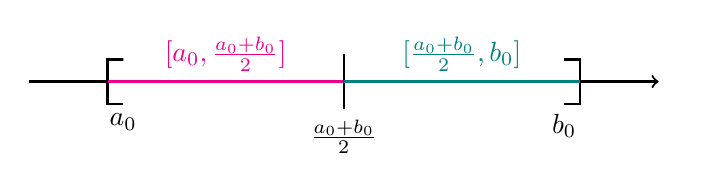
\begin{tikzpicture}
    \draw[thick,->] (0,0) -- (8,0) node[anchor= west]{};
    \draw[thick, color=black] (1,0) -- (1,8pt) -- (1.2,8pt) -- (1,8pt) -- (1,0) -- (1,-8pt) -- (1.2,-8pt) node[below]{$a_0$};
    \draw[thick, color=black] (7,0) -- (7,8pt) -- (6.8,8pt) -- (7,8pt) -- (7,0) -- (7,-8pt) -- (6.8,-8pt) node[below]{$b_0$};
    \draw[thick] (4,10pt) -- (4,-10pt) node[below]{$\frac{a_0 + b_0}{2}$};
    \draw[thick, color = magenta] (1,0) -- (4,0) -- (2.5,0) node[above]{$[a_0, \frac{a_0 + b_0}{2}]$};
    \draw[thick, color = teal] (4,0) -- (7,0) -- (5.5,0) node[above]{$[\frac{a_0 + b_0}{2}, b_0]$};
\end{tikzpicture}
\end{center}
\[A \cap [a_0, \frac{a_0 + b_0}{2}] \enspace \textrm{contiene infiniti elementi di} \enspace A \lor A \cap [\frac{a_0 + b_0}{2}, b_0] \enspace \textrm{contiene infiniti elementi di} \enspace A\] Ogni scelta non è necessariamente esclusiva, ma iterando la procedura si ottiene un intervallo di raggio sempre più piccolo i cui estremi superiore ed inferiore (essendo inclusi, $\max A$ e $\min A$) sono definiti da due successioni: 
\[\textrm{n-esima iterazione: } [a_n, b_n] \enspace con \enspace b_n - a_n = \frac{b_0 - a_0}{2^n}\]
$a_n$ è crescente, $b_n$ decrescente con $a_n < b_n$. Poiché $b_n \leq b_0$ in quanto monotona decrescente (dunque sempre minore o uguale del proprio valore iniziale) si ha $a_n < b_n \leq b_0$ ovvero $a_n$ succ. monotona crescente e superiormente limitata $\Rightarrow \enspace a_n \longrightarrow x_0$. Analogamente poiché $b_n$ monotona decrescente e $b_n > a_n$ $b_n$ converge a $x_0'$. Perciò:
\[b_n - a_n = \frac{b_0 - a_0}{2^n} \enspace per \enspace n \rightarrow \infty \enspace \lim b_n - \lim a_n = \lim b_n - a_n \enspace \Rightarrow \enspace x_0' - x_0 = 0 \Rightarrow x_0' = x_0\]
Poiché risulta $x_0 \in [a_n, b_n] \enspace \forall n$, $\forall r > 0 \enspace \exists n_1 > 0$ : $\forall n > n_1 \enspace [a_n, b_n] \subset I_r(x_0)$. Dunque:
\[I_r(x_0) \cap (A \setminus \{x_0\}) \supseteq [a_n, b_n] \cap (A \setminus \{x_0\})\]
Poiché $[a_n, b_n]$ contiene infiniti elementi di A, è verificato che $I_r(x_0) \cap (A \setminus \{x_0\}) \neq \emptyset$
\end{proof}
\hypertarget{corollaier}{
\begin{cor}
Ogni successione limitata $x_n \in \mathbb{R}$ ammette una sottosuccessione convergente $x_{n_k}$
\end{cor}}
\textbf{Nota: } $n_k : \mathbb{N} \longrightarrow \mathbb{N}$ successione crescente ($\mathbb{N} \subset \mathbb{R}$). $a_{n_k}$ sottosuccessione (dipende da $k$)
\begin{proof}
    Se $x_n$ è limitata (assume valori in un intervallo reale a estremi reali definiti), vi sono due possibilità:
    \begin{enumerate}
    \item $\#\{x_n\} < \infty$
    \item $\#\{x_n\} = \infty$
    \end{enumerate}
    1) Nel primo caso: $\{x_n\} = \{x_1, x_2, ... , x_N\}$ con $N \in \mathbb{N}$. Per infiniti $m \in \mathbb{N}$, deve essere $x_m = x_j$ per un certo $j \in \{1, ..., N\}$ (La successione può assumere solo un numero finito di valori, dunque per naturali tendenti a infinito dovrà assumere infinite volte il medesimo valore per numeri differenti). \newline Si pone $n_1 = \min \{m \in \mathbb{N}_+ : x_m = x_j\}$. Dall'osservazione precedente consegue che $\exists n_2 > n_1 : x_{n_2} = x_j$. \newline Iterando la costruzione si trova una successione crescente di numeri naturali $n_k$ tale che $x_{n_k} = x_j$ $\forall n \in \mathbb{N}_+$
    2) Nel secondo caso: l'insieme $\{x_n\}$ è infinito e limitato, quindi per il Teorema di Bolzano-Weierstrass ammette un punto di accumulazione $x_0 \enspace \Rightarrow \enspace \exists n_k$ successione crescente di numeri naturali:
    \[|x_{n_k} - x_0| < \frac{1}{k} \enspace \implies \enspace x_{n_k} \rightarrow x_0\]
\end{proof}

\subsubsection{Il teorema di Weierstrass}

\paragraph{Massimo e minimo: definizioni}
Sia $f : \enspace \mathbb{R} \longrightarrow \mathbb{R}$ e se ne indichi il dominio con $dom f$. Allora:
\begin{defin}
$f$ ha massimo se \[\exists x_M \in dom f : \enspace \forall x \in dom f \enspace f(x) \leq f(x_M)\]
\[ovvero \enspace f(x_M) = \max (Im f)\]
\end{defin}
\begin{defin}
$f$ ha minimo se \[\exists x_m \in dom f : \enspace \forall x \in dom f \enspace f(x) \geq f(x_m)\]
\[ovvero \enspace f(x_m) = \min (Im f)\]
\end{defin}

\paragraph{Insieme compatto}
\begin{defin}
$K \subset \mathbb{R}$ è compatto se è \underline{chiuso} ($\Leftrightarrow \mathbb{R} \setminus K$ aperto) e \underline{limitato} ($\Leftrightarrow \exists R > 0 : \enspace K \subset I_R(0)$)
\end{defin}
\hypertarget{weierstrass}{\begin{ther}[\textbf{Teorema di Weierstrass}]
Sia $f$ una funzione continua $^1$ definita su di un sottoinsieme compatto $^2$ di $\mathbb{R}$. 
Allora $f$ ha massimo e minimo.
\end{ther}}
\textbf{Nota bene: } è necessario siano soddisfatte entrambe le condizioni $^1$ e $^2$
\begin{proof}
    (1) Si dimostra innanzitutto che $Im f$ è limitata. Procedendo per assurdo: se $Im f$ non fosse limitata $\exists x_n \in K : \enspace |f(x_n)| \xrightarrow[n \rightarrow \infty]{} + \infty$ ($\square$).
    Poiché $x_n \in K \implies \enspace \{x_n\}$ limitata e $\{x_n\}$ infinito in quanto assume valori sempre diversi di modo che sia verificato ($\square$). Per il \hyperlink{corollaier}{corollario precedentemente dimostrato} $\exists x_{n_k} \rightarrow x_0 \in \mathbb{R}$. \newline Poiché $x_{n_k} \in K$ in quanto sottosuccessione di $x_n$, essendo K chiuso non può assumere valori superiori all'estremo sup, che fa parte dell'insieme ed è dunque $\max K$ $\implies \enspace x_0 \in K$. 
    \newline Dunque $|f(x_n)| \longrightarrow + \infty \enspace \implies \enspace |f(x_0)| \longrightarrow + \infty$ in quanto $f(x)$ continua su $K$ e dunque il limite del valore della funzione per una successione nel dominio tende al crescere dell'indice della successione al valore della funzione in corrispondenza del limite della s. Ma poiché $f$ continua e definita su $K$ per ipotesi, essa assume valori in $\mathbb{R}$ per $x \in K$ $\implies$ si ha l'assurdo $\implies$ è dimostrato che l'immagine è limitata. \newline 
    Dall'assioma di completezza consegue che $Im f$ ammette estremo superiore ed inferiore, dunque $\exists \inf(Im f)$, $\sup(Im f) \in \mathbb{R}$. \newline
    (2) Si verifica che $Im f$ abbia massimo e minimo: \newline
    Noto $\inf(Im f) \in \mathbb{R}$ :
    \[\inf(Im f) + \frac{1}{n} > \inf(Im f) \enspace \implies\]
    \[\implies \enspace \exists x_n \in K : \enspace \inf(Im f) \leq f(x_n) < \inf(Im f) + \frac{1}{n}\]
    Per il corollario: $\exists x_{n_k} \rightarrow x_0$
    \[\inf(Im f) \leq f(x_{n_k}) < \inf(Im f) + \frac{1}{n_k}\]
    in quanto $f$ continua. Per $k \rightarrow + \infty$ $f(x_n) \rightarrow f(x_0)$ e $\frac{1}{n_k} \rightarrow 0$ $\implies f(x_0) = \min \limits_K f$ in quanto $f(x_0) \in f(K)$ \newline Il massimo si tratta in modo analogo.
\end{proof}
\textbf{Nota: } $x_n$ si definisce \textit{successione minimizzante} - \textbf{non converge!}
\[\lim \limits_{n \rightarrow + \infty} f(x_n)= \inf(Im f)\]
\subsubsection{Teorema degli zeri}
\hypertarget{zeri}{\begin{ther}[\textbf{T. degli zeri}]
Sia $f$ una funzione continua. Siano $x_1, x_2 \in dom f$ con $x_1 < x_2$ e sia verificato $f(x_1) f(x_2) < 0$. Se $f$ è definita su $[x_1, x_2]$ allora \[\exists x_0 \in ]x_1, x_2[ : \enspace f(x_0) = 0\]
\end{ther}}
\begin{proof}
Si pongano $a_0 = x_1$, $b_0 = x_2$. \'E possibile supporre $f(a_0) < 0 < f(b_0)$ (qualora si considerasse $f(b_0) < 0 < f(a_0)$ il procedimento è analogo). \newline Si calcoli $f(\frac{a_0 + b_0}{2})$ . Vi sono tre possibilità:
\begin{itemize}[label=$\square$]
    \item $f(\frac{a_0 + b_0}{2}) = 0$ $\implies$ il teorema è dimostrato ($c = \frac{a_0 + b_0}{2}$)
    \item $f(\frac{a_0 + b_0}{2}) < 0$ $\implies$ si definiscono $a_1 = \frac{a_0 + b_0}{2}$; $b_1 = b_0$ con $f(a_1) < 0 < f(b_1)$ e $a_1 < b_1$ $\implies$ $b_1 - a_1 = \frac{b_0 - a_0}{2}$
    \item $f(\frac{a_0 + b_0}{2}) > 0$ $\implies$ si pone $a_1 = a_0$; $b_1 = \frac{a_0 + b_0}{2}$
\end{itemize}
Iterando: $a_n < b_n$, $a_n$ crescente e $b_n$ decrescente, $b_n - a_n = \frac{b_0 - a_0}{2^n}$ $\implies$ $\exists x_0 \in \enspace ]a_0, b_0[$ : $a_n, b_n \longrightarrow x_0$
\newline $f$ è continua $\implies$ $f(a_n) < 0 < f(b_n)$ per $n \rightarrow \infty$ : $f(x_0) \leq 0 \leq f(x_0)$ ed è quindi dimostrato per il confronto.
\end{proof}

\subsubsection{Teorema del valore intermedio}
\hypertarget{valint}{\begin{ther}[\textbf{T. del v. i.}]
Sia $f$ una funzione continua definita su un intervallo $I$. Siano $x_1 < x_2$ due punti di $I$ ed $y$ un punto compreso strettamente tra $f(x_1)$ e $f(x_2)$.\newline 
Allora esiste $x \in \enspace ]x_1, x_2[$ : $f(x) = y$.
\end{ther}}
\begin{proof}
Si costruisca la funzione ausiliaria $g(x) = f(x) - y$. Poiché per ipotesi $f(x_1) < y < f(x_2)$ si ha $g(x_1) g(x_2) = (f(x_1) - y)(f(x_2) - y) < 0$. Per il \hyperlink{zeri}{Teorema degli zeri} $\exists x_0$ compreso tra $x_1$ e $x_2$ t.c. 
\[0 = g(x_0) = f(x_0) - y \Longleftrightarrow f(x_0) = y\]
\end{proof}

\subsubsection{Continuità dell'inversa}
\hypertarget{inversa}{\begin{ther}
Sia $f$ funzione continua ed invertibile definita su di un intervallo ($f: \enspace I \rightarrow \mathbb{R}$ con $I \subset \mathbb{R}$). Allora $f^{-1} : f(\mathbb{R}) \rightarrow I$ è \underline{continua}.
\end{ther}}
\begin{proof}
\textbf{Nota preliminare:} è necessario che $f$ sia continua e definita su tutto l'intervallo considerato in quanto altrimenti, se esso fosse \underline{sconnesso}, $f^{-1}$ potrebbe risultare discontinua.
\begin{comment}\begin{center}
\begin{tikzpicture}
\begin{axis}[thick, xmin = 0, xmax = 8, ymin = -0.4, ymax = 4, axis x line = middle, axis y line = middle, ticks=none]
\draw[dashed] (axis cs:5.5,1) -- (axis cs:0,1) node[left]{$y_0$};
\draw[thick] (axis cs:1,0) -- (axis cs:4,1);
\draw[thick] (axis cs:5.5,3) -- (axis cs:9.5,6) node[right]{$f$};
\end{axis}
\end{tikzpicture}
\end{center}
\end{comment}
\textbf{(Procedimento 1)} Essendo $dom f^{-1} = im f$ per definizione: $\forall y \in dom f^{-1} \enspace \exists! x \in dom f : \enspace y = f(x)$.\\
Fissato $y_0 \in dom f^{-1}$, dunque $\exists! x_0 \in dom f : \enspace f(x_0) = y_0$. Fissato un $\varepsilon > 0$ a piacere per $x \in \enspace ] x_0 - \varepsilon, x_0 + \varepsilon[ \cap dom f$ $y = f(x)$ varierà in $]y_1, y_2[ \enspace \Leftrightarrow \enspace f^{-1} (]y_1, y_2[) \subset \enspace [x_0 - \varepsilon, x_0 + \varepsilon[$, ovvero l'inversa assumerà valori arbitrariamente vicini ad $x_0$ per valori di $y=f(x)$ arbitrariamente vicini ad $f(x_0)$, dunque per definizione di limite di funzione e continuità sarà continua sul proprio dominio, ovvero l'immagine di $f$. \\Ciò consegue dalla continuità di $f(x)$.
\\ \\
\textbf{(Procedimento 2)} Dalle ipotesi è innanzitutto possibile dedurre le seguenti implicazioni: \begin{itemize}[label=$\cdot$]
    \item  $f: \enspace I \rightarrow \mathbb{R}$ continua e invertibile su $I$ $\implies$ $f$ strettamente monotona sull'intervallo
    \item $f$ invertibile $\implies$ $f$ iniettiva: $f(x_1) = f(x_2) \Rightarrow x_1 = x_2$
\end{itemize} 
Si consideri quindi il sottointervallo $]x_1, x_2[ \subset I$. Posto per assurdo $f$ non sia strettamente crescente sull'intervallo, si abbia che la funzione assuma un valore, sia $f(x_3) \in \enspace ]f(x_1), f(x_2)[$ su di un punto del dominio esterno al sottointervallo $x_3 > x_2 \implies x_3 \notin ]x_1, x_2[$, per il \hyperlink{valint}{Teorema del Valore intermedio} $\exists \overline{x} \in \enspace ]x_1, x_2[$ : $f(\overline{x) = f(x_3)}$. Ma poiché $\overline{x} \in \enspace ]x_1, x_2[$, si avrebbe l'assurdo con la contraddizione dell'ipotesi di iniettività (condizione necessaria per l'invertibilità), in quanto $f$ assumerebbe il medesimo valore per due punti diversi del dominio.
\end{proof}
\textbf{Nota:} la validità del teorema di continuità dell'inversa conferma la nozione intuitiva di continuità di una curva, che, se verificata dal 'punto di vista' di un asse lo è anche rispetto all'altro.

\paragraph{Conseguenze del teorema}
Ne consegue che, \hyperlink{elementarii}{dimostrata la continuità delle funzioni elementari}:\\ \begin{center}$\sqrt[n]{x} \enspace e^x \enspace \arcsin{x} \enspace \arccos{x} \enspace \arctan{x}$ sono continue.\end{center}

\subsubsection{Teorema della permanenza del segno}
\label{subsubsec:perman}
\begin{ther}[\textbf{T. p. s.}]
Siano $f$ continua, $x_0 \in dom f$ t.c. $f(x_0) > 0$. Allora
\[\exists \delta > 0 : \enspace \forall x \in I_{\delta}(x_0) \cap dom f \enspace f(x) > 0\]
Analogamente se $f(x_0) < 0$
\[\exists \delta > 0 : \enspace \forall x \in I_{\delta}(x_0) \cap dom f \enspace f(x) < 0\]
\end{ther}
\begin{proof}
Sia $\varepsilon = \frac{f(x_0)}{2}$. Dalla definizione di funzione continua si ha che 
\[\exists \delta > 0 : \enspace \forall x \in I_{\delta}(x_0) \cap dom f \enspace f(x) \in I_{\varepsilon}(f(x_0))\]
Dunque $f(x) > f(x_0) - \varepsilon$ in quanto assume valori strettamente contenuti nell'intorno circolare di raggio $\varepsilon$; avendo posto $\varepsilon = \frac{f(x_0)}{2}$, si ha \[f(x) > \frac{f(x_0)}{2}\] Poiché per ipotesi $f(x_0) > 0$ $\implies$ $f(x) > 0$ per valori di $x$ nell'intorno circolare di raggio $\delta$ di $x_0$.
\end{proof}

\section{Derivate}

\subsection{Simboli di Landau}
\begin{defin}[\textbf{O grande}]
Siano $f$ e $g$ due funzioni definite in un intorno di $x_0 \in \mathbb{R}$. Se
\[\lim \limits_{x \rightarrow x_0} \frac{f(x)}{g(x)} = l \in \mathbb{R}\] si dice che $f$ è \underline{controllata} da $g$ per $x$ tendente a $x_0$. Si utilizza la notazione:
\[f = O(g) \quad \textrm{per} \enspace x \rightarrow x_0\]
Alternativamente si può quindi dire che $f$ è \textit{un $O$ grande di $g$ per $x$ tendente a $x_0$}.\\
Si noti che è possibile esprimere la medesima relazione rifacendosi alla definizione di limite:
\[\forall I_r(x_0) \enspace \exists C > 0 : \enspace \forall x \in I_r(x_0)\]
\[|f(x)| \leq C |g(x)|\]
\end{defin}

\begin{defin}[\textbf{o piccolo}]
Siano $f$ e $g$ due funzioni definite in un intorno di $x_0 \in \mathbb{R}$. Se
\[\lim \limits_{x \rightarrow x_0} \frac{f(x)}{g(x)} = 0\] si dice che $f$ è \underline{trascurabile} rispetto a $g$ per $x$ tendente a $x_0$. Si utilizza la notazione:
\[f = o(g) \quad \textrm{per} \enspace x \rightarrow x_0\]
Alternativamente si può quindi dire che $f$ è \textit{un $o$ piccolo di $g$ per $x$ tendente a $x_0$}.
\end{defin}

\paragraph*{Note e Algebra degli $o$}
\begin{itemize}[label=$\ast$]
\item Se una funzione $f(x)$ è trascurabile rispetto ad un'altra $g(x)$ per $x \rightarrow 0$, dunque $f(x) = o(g(x))$, ciò equivale al fatto che $f(x)$ sia un \underline{infinitesimo di ordine superiore} rispetto a $g(x)$ (va a 0 più rapidamente).
\item L'$o$ piccolo fornisce un'informazione più generica rispetto all'$O$ grande.
\item $o(x^n) + o(x^m) = o(x^n)$ per $x \rightarrow x_0$ se $n < m$ \\ in quanto la potenza di esponente maggiore tende più rapidamente a 0, e dunque una funzione trascurabile rispetto ad essa lo sarà anche rispetto ad una potenza di esp. minore.
\item $\lambda o(x^n) = o(\lambda x^n) = o(x^n)$ se $\lambda \neq 0$ \hypertarget{opiccoli}{*}
\item $x^m o(x^n) = o(x^{m+n})$
\item $o(x^m) o(x^n) = o(x^{m+n})$
\item $[o(x^n)]^k = o(x^{kn})$
\end{itemize}

\subsection{Asintoti}
\begin{defin}
Sia $f$ funzione. 
Se $f$ definita su $I_A(+ \infty)$ con $A \in \mathbb{R}_+$, $\lim \limits_{x \rightarrow + \infty} f(x) = + \infty$ ed essa tende ad un andamento lineare per valori arbitrariamente grandi di $x$, ovvero:
\[\lim \limits_{x \rightarrow + \infty} \{f(x) - (mx + q)\} = 0\]
con $m, q \in \mathbb{R}$. In notazione di Landau:
\[f(x) = mx +q + o(1) \quad \textrm{per} \enspace x \rightarrow + \infty\]
Si definisce $g(x) = mx + q$ \underline{asintoto destro} di $f$.\\ Analogamente si definisce l'asintoto \underline{sinistro} per $f$ tendente ad un andamento lineare per $x \rightarrow - \infty$.\\
Se $m \neq 0$, l'asintoto si dice \underline{obliquo}, altrimenti se $m = 0$ \underline{orizzontale}. 
\end{defin}

\paragraph*{Determinare i parametri dell'asintoto}
\[m = \lim \limits_{x \rightarrow \pm \infty} \frac{f(x)}{x} \enspace | \enspace q = \lim \limits_{x \rightarrow \pm \infty} (f(x) - mx)\]

\subsection{Definizione di derivata}
\begin{defin}[\textbf{(Derivata - 1)}] Sia data $f : \enspace \mathbb{R} \rightarrow \mathbb{R}$ e un punto del dominio $x_0 \in dom f$. $f$ si dice \underline{derivabile} in $x_0$ se $\exists a \in \mathbb{R}$ :
\[f(x) = f(x_0) + a(x-x_0) + o(x-x_0) \quad \textrm{per} \enspace x \rightarrow x_0\]
Se dunque esiste tale $a$, si definisce \underline{derivata di $f$ in $x_0$}. Si indica equivalentemente come:
\[a = f'(x_0) = f^{(1)}(x_0) = Df(x_0) = \dot{f}(x_0) = \frac{df}{dx}(x_0)\]
La quarta notazione è detta \underline{di Newton} ed è specificamente usata per le derivate delle variabili meccaniche rispetto al \underline{tempo}; la quinta è invece detta notazione \underline{di Leibniz}.
\end{defin}

\paragraph{Significato geometrico} 
La derivata corrisponde al coefficiente angolare della retta che approssima l'andamento della funzione in un intorno del punto $x_0$, a meno di un termine di errore trascurabile per $x \rightarrow x_0$, ovvero l'\textit{o piccolo di $x - x_0$}.
Tale significato è ben evidenziato anche nella definizione \"classica\" di derivata:
\begin{defin}[\textbf{(Derivata - 2)}] Si consideri una funzione ed un punto $x_0$ analogamente alla prima definizione. La derivata di $f$ in $x_0$ è definita dal \underline{limite del rapporto incrementale} della funzione per $x \rightarrow x_0$:
\[f'(x_0) = \lim \limits_{x \rightarrow x_0} \frac{f(x) - f(x_0)}{x - x_0}\]
\end{defin}

\subsubsection{Funzioni derivabili}
\label{subsubsec:derivabili}
\begin{defin}
Una funzione $f$ si dice \underline{derivabile} se lo è per tutti i punti del dominio
\end{defin}
\begin{prop}
Le funzioni derivabili sono continue
\end{prop}
\begin{proof}
Se $f$ è derivabile, per un qualsiasi punto del dominio $x_0$ si avrà $f(x) = f(x_0) + f'(x_0) (x - x_0) + o (x- x_0)$ per $x \rightarrow x_0$. Dunque passando al limite per $x$ a $x_0$ si avrà l'annullamento del termine dipendente da $(x-x_0)$ e dell'\textit{o piccolo}, che per definizione tende ad annullarsi con la medesima rapidità (infinitesimo di ordine superiore a $(x - x_0)$ per $(x - x_0) \rightarrow 0$):
\[\lim \limits_{x \rightarrow x_0} f(x) = \lim \limits_{x \rightarrow x_0} f(x_0) + f'(x_0) (x - x_0) + o (x- x_0) = f(x_0) + 0 = f(x_0)\]
Dunque $f$ risulta continua per definizione.
\end{proof}
\textbf{Nota bene:} L'implicazione contraria \underline{è falsa}. Ovvero, tutte le funzioni derivabili sono continue ma \underline{non tutte} le funzioni continue sono derivabili. In altri termini, l'insieme delle funzioni derivabili (una volta, ma di conseguenza anche per derivate di ordine superiore) è sottoinsieme proprio dell'insieme delle funzioni continue.
Ad esempio $f(x) = |x|$ è continua su tutta la retta ma in $x_0 = 0$ non è derivabile, in quanto per $x$ tendente a $x_0$ da destra o da sinistra sono determinati valori differenti della derivata.

\subsection{Regole di Calcolo delle derivate}
\begin{prop}
Siano $f$ e $g$ funzioni derivabili. Si ha:
\[D(f + g) = Df + Dg \enspace | \enspace D(f-g) = Df - Dg \enspace | \enspace D(f \cdot g) = (Df) \cdot g + f \cdot (Dg)\] \[D \bigg(\frac{1}{g}\bigg) = - \frac{Dg}{g^2} \enspace | \enspace D \bigg(\frac{f}{g}\bigg) = \frac{g \cdot Df - f \cdot Dg}{g^2}\]
La formula per la derivata del prodotto è detta \underline{F. di Leibniz}. Si noti inoltre che tali derivate sono calcolabili solo in punti in cui entrambe le funzioni siano continue e derivabili.
\end{prop}
\begin{proof}
Si studia in corrispodenza di $x_0 \in dom f \cap dom g$
\textbf{Somma algebrica} $f(x) = f(x_0) + f'(x_0) (x-x_0) + o (x - x_0)$, $g(x) = g(x_0) + g'(x_0) (x-x_0) + o (x - x_0)$. Sommando: $(f+g)(x) = f(x) + g(x) = (f+g)(x_0) + (f'(x_0) + g'(x_0)) (x-x_0) + o (x-x_0)$. Dunque il termine di derivata è $Df(x_0) + Dg(x_0) = D(f+g)(x_0)$. Analogamente per la differenza.
\textbf{Prodotto} $f(x) \cdot g(x) = (f\cdot g)(x_0) + [f'(x_0)g(x_0) + f(x_0)g'(x_0)](x-x_0) + o(x -x_0)$ (i termini moltiplicati per l'$o$ piccolo sono assorbiti, mentre il prodotto tra due $o$ piccoli e l'$o((x-x_0)^2)$ è trascurabile rispetto a quello di primo grado. Dunque $(f\cdot g)'(x_0) = f'(x_0)g(x_0) + f(x_0)g'(x_0)$
\textbf{Reciproco e rapporto} 
\[\frac{1}{g(x)} = \frac{1}{g(x_0) + g'(x_0) (x-x_0) + o(x-x_0)} = \frac{1}{1 + \frac{g'(x_0)(x -x_0) + o(x-x_0)}{g(x_0)}} = \frac{1}{1+h(x)}\]
Con $h(x) \rightarrow 0$ per $x \rightarrow x_0$. Sviluppando $\frac{1}{1+h(x)} = 1 - h(x) + o(h(x))$ per $x \rightarrow x_0$. Dunque
\[\frac{1}{g(x)} = \frac{1}{g(x_0)}\bigg[1 - \frac{g'(x_0)(x-x_0) + 0(x-x_0)}{g(x_0)} \bigg] = \frac{1}{g(x_0)} - \frac{g'(x_0)}{g^2(x_0)}(x-x_0) + o(x-x_0)\]
(valgono le consuete considerazioni per $o$) dunque
\[D\frac{1}{g} = -\frac{Dg}{g^2} \enspace \implies \enspace D\bigg(\frac{f}{g}\bigg) = \frac{Df}{g} - \frac{fDg}{g^2} = \frac{gDf - f Dg}{g^2}\]
\end{proof}

\textbf{Nota} L'operatore di derivazione $D$ è lineare:
\[D ( \lambda f + \mu g) = \lambda D f + \mu D g\]

\subsection{Derivata di f. composta}
\begin{prop}
Siano $f$, $g$ funzioni derivabili. Allora la derivata di $f$ composto $g$: 
\[D (f (g(x) ) = D ((f \circ g)(x)) = (D f)(g(x)) \cdot D g(x) = \frac{\textrm{d}f}{\textrm{d}g}\frac{\textrm{d}g}{\textrm{d}x}\]
ovvero al prodotto tra la derivata di $g$ in $x$ e la derivata di $f$ in $g(x)$.
\end{prop}
\begin{proof}
\[(f\circ g)(x_0) = f(g(x_0)) \enspace ; \enspace f(g(x)) = f(g(x_0)) + (Df)(g(x_0)) (g(x) - g(x_0)) + o(g(x) - g(x_0)) \enspace \textrm{per } x \rightarrow x_0 \implies g(x) \rightarrow g(x_0)\]
L'implicazione consegue dalla continuità di $g$ (per ipotesi derivabile, dunque continua). Per $x \rightarrow x_0$ si ha $g(x) - g(x_0) = Dg(x_0) (x - x_0) + o(x-x_0)$ e dunque $o(g(x) - g(x_0)) = o(Dg(x_0) (x - x_0) + o(x-x_0)) = 0\big((x-x_0)[Dg(x_0) + o(1)]\big) = Dg(x_0)o(x-x_0) = o(x-x_0)$ (per \hyperlink{opiccoli}{l'algebra degli $o$}). Si è quindi verificato $o(g(x) - g(x_0)) = o(x-x_0)$
\\Avendo inoltre $Df(x_0) \cdot o(x-x_0) = o(x-x_0)$ si ottiene:
\[(f\circ g)(x_0) = f(g(x_0)) + (Df)(g(x_0))(Dg(x_0))(x-x_0) + o(x-x_0) \enspace \textrm{per } x \rightarrow x_0\]
Si ha quindi $D(f\circ g) (x_0) = (Df)(g(x_0))(Dg(x_0))$
\end{proof}

\subsection{Derivata dell'inversa}
\begin{prop}
Sia $f$ derivabile ed invertibile sul dominio o su di un intervallo in esso contenuto. Si supponga $f^{-1}$ sia derivabile. Allora:
\[D f^{-1}(y) = \frac{1}{D f (f^{-1}(y))}\]
ovvero al reciproco della derivata di $f$ in corrispondenza del valore dell'inversa di $y$.
\end{prop}
\begin{proof}
Per definizione $(f^{-1} \circ f)(x) = x$. Dunque $D\big[f^{-1}(f(x))\big] = Dx = 1$. Per la regola di composta $D\big[f^{-1}(f(x))\big] = (Df^{-1})(f(x)) \cdot Df(x) = 1$ $\implies$ $(Df^{-1})(f(x)) = \frac{1}{Df(x)}$.
\\Considerando $y = f(x) \Leftrightarrow x = f^{-1}(y)$ si ha $(Df^{-1})(f(x)) = (Df^{-1})(y)$ e $Df(x) = Df(f^{-1})(x)$; operando le opportune sostituzioni la dimostrazione è conclusa.
\end{proof}

\begin{ther}[\textbf{(della funzione / applicazione inversa)}]
Sia $f : \enspace \mathbb{R} \rightarrow \mathbb{R}$ derivabile con derivata $f'$ continua. Si fissi un punto del dominio $x_0 \in dom f$, e si supponga $D f (x_0) \neq 0$. Allora\\
$\exists \delta > 0 : \enspace f\restriction_{I_\delta(x_0)}$ \underline{è invertibile} (ammette inversa) e $f^{-1} : f( I_\delta(x_0)) \rightarrow \mathbb{R}$, ovvero la funzione inversa definita sull'immagine dell'intorno circolare a valori reale, \underline{è derivabile}.
\end{ther}

\subsection{Calcolo di derivate}
$f(x) = c$ (costante). Applicando la definizione:
    \[f'(x_0) = \lim \limits_{x \rightarrow x_0} \frac{f(x) - f(x_0)}{x - x_0} = \lim \limits_{x \rightarrow x_0} \frac{c - c}{x - x_0} = 0\]
    Intuitivamente, il grafico di una funzione costante è una retta parallela all'asse delle ascisse, dunque approssimata (perfettamente) in qualsiasi punto del dominio da una retta a coefficiente angolare nullo.
    \\$f(x) = x^n$ con $n \in \mathbb{N}_+$ (potenza). $f'(x) = n x^{n-1}$. Considerando il primo caso: $c = c \cdot x^0$ $\implies$ $D(x^0) = 0$
    \\$f(x) = \sum \limits_{j = 0}^{n} a_j x^j$ (polinomio) Consegue dalla precedente: $f'(x) = \sum \limits_{j = 0}^{n} a_j j x^{j-1}$
    \\$f(x) = \sin x$ $f'(x) = \cos x$ $\bigg|$ $f(x) = \cos x$ $f'(x) = -\sin x$ $\bigg|$ $f(x) = \tan x$ $f'(x) = 1 + \tan^2 x$
    \\$f(x) = e^x$ $f'(x) = e^x$ $\bigg|$ $f(x) = \alpha^x$ $f'(x) = \log(\alpha) \alpha^x$
    \\\textbf{Inverse:}
    \[f(x) = \arcsin x \enspace f'(x) = \frac{1}{\sqrt{1 - x^2}} \enspace \bigg| \enspace f(x) = \arccos x \enspace f'(x) = - \frac{1}{\sqrt{1 - x^2}}\]
    \[f(x) = \arctan x \enspace f'(x) = \frac{1}{1 + x^2} \enspace \bigg| \enspace f(x) = \log x \enspace f'(x) = \frac{1}{x}\]


\section{Teoremi sulle derivate}
\subsection{Teorema di Rolle}
\begin{ther}
Si consideri una funzione definita e continua sull'intervallo chiuso $[a,b]$ a valori reali ($f : \enspace \enspace [a, b] \rightarrow \mathbb{R}$) e derivabile sull'aperto $]a, b[$. Allora:
\[f(a) = f(b) \enspace \Longrightarrow \enspace \exists c \in \enspace ]a, b[ \enspace : \enspace Df(c) = 0\]
Ovvero se il valore assunto dalla funzione nei due estremi dell'intervallo è uguale, esiste almeno un punto nell'aperto in cui la derivata della funzione sia nulla.
\end{ther}
\textbf{Nota bene:} Non è necessariamente valida l'implicazione contraria: la coincidenza della funzione su a e b è condizione sufficiente ma non necessaria per l'esistenza di un punto a derivata nulla nell'aperto; dunque è possibile sia verificata la seconda senza che lo sia la prima: difatti sono punti critici anche i p. di flesso.
\begin{proof}
Essendo soddisfatte le ipotesi del \hyperlink{weierstrass}{Teorema di Weierstrass}, si ha innanzitutto che $f$ ammette massimo e minimo in $[a, b]$. Si presentano due casi:
\textbf{(i) Il massimo ed il minimo sono raggiunti in $a$ e $b$} Ciò implica che i valori assunti dalla funzione sull'intervallo siano compresi tra $f(a)$ e $f(b)$; essendo per ipotesi $f(a) = f(b)$ la funzione risulta dunque costante. Perciò esistono infiniti punti nell'intervallo soddisfacenti la condizione della tesi, in quanto la derivata di costante è nulla in ogni punto. \\
\textbf{(ii) Almeno uno dei due è raggiunto in un punto dell'aperto} ovvero diverso dagli estremi, sia $x_0 \in \enspace ]a, b[$.
Si consideri il caso in cui esso sia un punto di minimo (il procedimento è analogo per il massimo): per definizione si ha che $\forall x \in \enspace [a, b] \enspace f(x) \geq f(x_0)$. Si determina la derivata della funzione nel punto $x_0$, noto che per ipotesi è derivabile sull'aperto, tramite il limite dell'incrementale da sinistra e destra:
\[D f(x_0) = \lim \limits_{x \rightarrow x_0^-} \frac{f(x) - f(x_0)}{x - x_0}\]
Si ha dunque al numeratore un termine $\geq 0$, al denominatore uno $< 0$ (limite da sx): il limite è quindi $\leq 0$.
\[D f(x_0) = \lim \limits_{x \rightarrow x_0^+} \frac{f(x) - f(x_0)}{x - x_0}\]
Si ha dunque al numeratore un termine $\geq 0$, al denominatore uno $> 0$ (limite da sx): il limite è quindi $\geq 0$.
Applicando il teorema del confronto (in quanto la derivata è determinata e unica nel punto) \hypertarget{confr}{(***)}, si ha: $0 \leq Df(x_0) \leq 0$  dunque \[Df(x_0) = 0\]
$x_0$ soddisfa la condizione del punto ricercato $c$.
\end{proof}

\subsection{Piccolo Teorema di Fermat}
Si introduce innanzitutto il concetto di punto critico:
\begin{defin}
\label{critico}
Sia $f$ derivabile su di un intervallo. Allora un dato $x_0 \in \enspace dom f$ si definisce \underline{punto critico} se $f'(x_0) = 0$.
\end{defin}

\begin{ther}[\textbf{Piccolo T. di F.}]
Sia $f: \enspace ]a, b[ \rightarrow \mathbb{R}$ (funzione definita sull'aperto a valori reali); si supponga $f$ sia derivabile e abbia in $x_0 \in \enspace ]a, b[$ un \underline{massimo locale} o \underline{minimo l.}. Allora \[f'(x_0) = 0\]
\end{ther}
\textbf{Nota bene:} \underline{Non è valida l'implicazione contraria}: è possibile si verifichi l'annullamento della derivata anche in corrispondenza di un punto di flesso.
\begin{proof}
Si dimostra applicando il confronto come effettuato nella dimostrazione precedente \hyperlink{confr}{(***)}.
\end{proof}

\begin{cor}[\textbf{(al teorema di Rolle}] Sia $f$ derivabile in $I_r(x_0)$ con $f'$ continua in $x_0$. Se $f'(x_0) \neq 0$ allora esiste un intorno del punto $x_0$ contenuto strettamente in quello di raggio $r$ su cui la funzione risulta iniettiva: $\exists \delta \in \enspace ]0, r[\enspace : \enspace f: \enspace I_\delta(x_0) \xrightarrow{1-1} \mathbb{R}$.
\end{cor}
\begin{proof}
Si procede per assurdo, negando la tesi: $\forall \delta \enspace \exists x_\delta, y_\delta \in I_\delta(x_0), x_\delta \neq y_\delta : \enspace f(x_\delta) = f(y_\delta)$ (si nega l'iniettività su qualsiasi intorno di raggio $\delta$ piccolo a piacere). Si studia dunque $f\restriction_{[x_\delta, y_\delta]}$: \\Poiché per costruzione $[x_\delta, y_\delta] \subset \enspace [a, b[$, essendo $f$ continua (1) e derivabile (2) su tutto l'aperto lo è anche sul sottointervallo. Per costruzione $f(x_\delta) = f(y_\delta)$ (3): sono quindi soddisfatte le tre ipotesi del teorema di Rolle in $[x_\delta, y_\delta]$. Dunque applicandolo si ha che $\exists z_\delta \in \enspace ]x_\delta, y_\delta[$ t.c. $f'(z_\delta) = 0$. Per costruzione $[x_\delta, y_\delta] \subset I_\delta(x_0)$, dunque $z_\delta \in I_\delta(x_0)$. Se si fa tendere $\delta \rightarrow 0^+$, si ha quindi $z_\delta \rightarrow x_0$ in quanto appartiene all'intervallo di raggio $\delta$ indipendentemente dal valore assunto dal parametro, poiché avendo negato la tesi di iniettività sono sempre soddisfatte le ipotesi di Rolle. Essendo $f'$ continua sull'aperto, lo è anche in $I_\delta(x_0)$ in esso contenuto: si ha quindi $\lim \limits_{z_\delta \rightarrow x_0} f'(z_\delta) = f'(x_0)$. Ma poiché per Rolle si ha $f'(z_\delta) = 0$ mentre per ipotesi $f'(x_0) \neq 0$, si ha l'assurdo. La tesi è quindi dimostrata.
\end{proof}
\textbf{Nota sulla dim:} L'ipotesi di continuità della derivata è necessaria per la validità del corollario. infatti:
\begin{oss} Se una funzione ha derivata continua sul dominio, allora è derivabile sul dominio. Viceversa una funzione derivabile sul dominio non ha necessariamente derivata continua sul medesimo.\\
\textbf{Esempio:}
\[f(x) = \begin{cases}
  x + 2 x^2 sin(\frac{1}{x}) &{per} \enspace x \neq 0 \\
  0 &{per} \enspace x = 0
\end{cases}\]
\end{oss}

\subsection{Teorema di Lagrange}
\begin{ther}[\textbf{T. di L.}]
Sia \begin{enumerate}
    \item $f: \enspace \enspace [a, b] \rightarrow \mathbb{R}$ (definita sul chiuso a valori reali) e continua sul chiuso
    \item $f$ derivabile sull'aperto $]a, b[$
\end{enumerate}
Allora esiste un almeno un punto dell'aperto in cui la derivata ha il medesimo valore del rapporto incrementale della funzione tra $a$ e $b$ (ovvero il coefficiente angolare della secante):
\[\exists c \in \enspace ]a, b[ \enspace : \enspace f'(c) = \frac{f(b) - f(a)}{b - a}\]
\end{ther}
\begin{proof}
Si costruisca la funzione ausiliaria $h(x)$, definita come:
\[h(x) = f(x) - [f(a) + \frac{f(b) - f(a)}{b - a}(x - a)]\]
Si ha innanzitutto $h(a) = h(b) = 0$; inoltre $h$ ha la medesima regolarità di $f$. Essendo somma algebrica di funzioni continue (l'incrementale tra a e b è un coefficiente fisso, dunque il termine tra quadri è una funzione polinomiale di primo grado, continua su tutta la retta; $f$ continua sul chiuso per ipotesi) \underline{$h(x)$ è continua sul chiuso}; inoltre essendo $f$ derivabile sull'aperto per ipotesi e il termine polinomiale analogamente derivabile sulla retta, \underline{$h(x)$ è derivabile sull'aperto}. Sono soddisfatte le ipotesi del Teorema di Rolle, dunque:
\[\exists c \in \enspace]a, b[\enspace : \enspace h'(c) = 0\]
Per l'algebra delle derivate $D h(x) = D f (x) - \frac{f(b) - f(a)}{b - a}$, quindi:
\[0 = D f (c) - \frac{f(b) - f(a)}{b - a} \enspace \implies \enspace D f (c) = \frac{f(b) - f(a)}{b - a}\]
\end{proof}
\begin{oss}
La costruzione della funzione ausiliaria, ottenuta sottraendo a $f$ la secante per i punti in corrispondenza degli estremi dell'intervallo, permette di effettuare un \textit{cambiamento di sistema di riferimento}, una trasformazione che preserva le caratteristiche della funzione riconducendosi al contempo al caso di applicazione del teorema di Rolle.
\end{oss}

\begin{cor}
\label{corlagrange}
Siano poste le medesime ipotesi del teorema. Allora:
\begin{enumerate}[label=$\square$]
    \item se $f'(x) = 0 \forall x \in \enspace ]a, b[$ $\implies$ $f$ costante
    \item se $f'(x) > 0 \forall x \in \enspace ]a, b[$ $\implies$ $f$ strettamente / monotona crescente
    \item se $f'(x) < 0 \forall x \in \enspace ]a, b[$ $\implies$ $f$ strettamente / monotona decrescente
\end{enumerate}
\end{cor}
\begin{proof}
(i) Sia, a fini di praticità, $I = [a, b]$. Siano quindi $x_1, x_2 \in I$, con $x_1 < x_2$. Per il teorema di Lagrange dunque $\exists c \in \enspace ]x_1, x_2[ \enspace : \enspace f(x_2) - f(x_1) = f'(c)(x_2 - x_1)$\\
Ma essendo $f'(c) = 0$ in quanto nulla per ogni $x \in I$, si ha $f(x_1) = f(x_2) \forall x_1, x_2 \in I$ (l'ordinamento totale dei reali garantisce sia possibile applicare la procedura dati due punti distinti qualsiasi), dunque per definizione $f$ è costante sull'intervallo.\\
(ii) Sia analogamente $x_1 < x_2$; applicando Lagrange $\exists c \in \enspace ]x_1, x_2[ \enspace : \enspace f(x_2) - f(x_1) = f'(c)(x_2 - x_1)$\\
Il secondo termine è positivo; se $f'(c) \geq 0$ per ogni punto nell'aperto, il primo membro dell'equazione risulta positivo, ovvero:
\[f(x_2) - f(x_1) \geq 0 \implies f(x_2) \geq f(x_1)\]
Dunque la funzione è strettamente crescente.
(iii) Si procede in modo affine a (ii) per il caso a derivata negativa.
\end{proof}
\textbf{Nota sulla dimostrazione} \'E necessario che l'insieme di definizione sia un intervallo, ovvero sia connesso.

\subsection{Teorema di Cauchy}
\label{subsec:cauchy}
\begin{ther}
Siano $f,g : \enspace [a, b] \rightarrow \mathbb{R}$ continue sul chiuso e derivabili sull'aperto. Allora $\exists c \in \enspace ]a, b[$ :
\[f'(c)(g(b) - g(a)) = g'(c)(f(b) - f(a))\]
\end{ther}
\textbf{Nota:} il Teorema di Lagrange risulta essere il caso particolare in cui $g(x) = x$ :
\[f'(c)(g(b) - g(a)) = f'(c)(b - a) = g'(c)(f(b) - f(a)) = 1 \cdot (f(b) - f(a)) \implies f'(c) = \frac{f(b) - f(a)}{b - a}\]
\begin{proof}
Si costruisca la funzione ausiliaria $h$:
\[h(x) = (f(x) - f(a)) (g(b) - g(a)) - (g(x) - g(a)) (f(b) - f(a))\]
Si ha innanzitutto $h(a) = 0 \cdot (g(b) - g(a)) - 0 \cdot (f(b) - f(a)) = 0 = h(b)$; inoltre $h$ ha la medesima regolarità di $f$ e $g$. Poiché $f$, $g$ continue sul chiuso per ipotesi, e i termini $f(a), f(b), ...$ sono coefficienti reali, $h$ risulta continua in quanto combinazione lineare di continue. Analogamente si verifica la derivabilità sull'aperto. Sono dunque soddisfatte le ipotesi del Teorema di Rolle: si ha quindi $\exists c \in \enspace ]a, b[$ : $h'(c) = 0$. Derivando quindi $h$, noto che la derivata dei coefficienti è nulla: $h'(x) = (g(b) - g(a)) f'(x) - (f(b) - f(a)) g'(x)$ $\implies$ $0 = h'(c) = (g(b) - g(a)) f'(c) - (f(b) - f(a)) g'(c)$ $\implies$ $(g(b) - g(a)) f'(c) = (f(b) - f(a)) g'(c)$
\end{proof}

\subsection{Teorema di invertibilità locale}
\begin{ther}
Sia $f : \enspace ]a, b[ \rightarrow \mathbb{R}$ (definita sull'aperto) derivabile con derivata continua $^1$. Se $\exists x_0 \in \enspace ]a, b[ \enspace : f'(x_0) \neq 0$ allora $\exists \delta > 0 : \enspace I_\delta(x_0) \subset \enspace ]a, b[$ tale che
\[f^{-1} : f(I_\delta(x_0)) \rightarrow I_\delta(x_0)\] è derivabile e $\forall y \in f(I_\delta(x_0))$ \[D f^{-1}(y) = \frac{1}{(Df) (f^{-1}(y))}\]
\end{ther}
\textbf{$^1$} tale ipotesi è definita \textit{i. di struttura}. Si noti che l'assumere $f'$ continua implica $f$ derivabile e dunque $f$ continua; vedasi in merito \hyperref[subsubsec:derivabili]{l'osservazione sulla definizione di funzione derivabile}.
\begin{proof}
Nella dimostrazione del corollario del T. di Rolle si è già provato che, dato un punto del dominio di una funzione, è possibile trovare un $\delta > 0$ tale per cui attuando una restrizione del dominio ad un intorno di raggio $\delta$ di tale punto essa risulta iniettiva. Dal teorema della \hyperlink{inversa}{continuità dell'inversa} si ha che dalla continuità di $f$ consegue quella di $f^{-1}$ sull'immagine dell'intervallo di definizione della prima; poiché si è assunto per ipotesi $f'(x) \neq 0$ e la derivata è continua, per il \hyperref[subsubsec:perman]{il teorema della permanenza del segno} esiste un $\delta > 0$ opportunamente piccolo tale che la derivata risulti diversa da zero per ogni punto del dominio in un intorno di $x_0$ di raggio $\delta$. \\
Si fissi quindi $\overline{y} \in f(I_\delta(x_0))$. Allora $\exists! \overline{x} \in I_\delta(x_0)$ t.c. $f(\overline{x}) = \overline{y}$ ($f$ iniettiva e invertibile). Essendo per ipotesi $f$ derivabile sull'aperto e dunque anche sull'intorno in esso contenuto propriamente, per definizione di derivata:
\[f(x) = f(\overline{x}) + f'(\overline{x}) (x - \overline{x}) + o (x - \overline{x}) \quad \textrm{per} \enspace x \rightarrow \overline{x}\]
Posto $y = f(x)$ si ha $y = \overline{y} + f'(\overline{x}) (x - \overline{x}) + o (x - \overline{x})$ $\Leftrightarrow$ $f^{-1}(y) = f^{-1}(\overline{y}) + f'(f^{-1}(\overline{y})) (f^{-1}(y) - f^{-1}(\overline{y})) + o (x - \overline{x}) \quad \textrm{per} \enspace f^{-1}(y) \rightarrow f^{-1}(\overline{y})$
\\Dunque isolando opportunamente:
\[f^{-1}(y) = f^{-1}(\overline{y}) + \frac{1}{f'(f^{-1}(\overline{y}))}(y - \overline{y}) + \frac{1}{f'(f^{-1}(\overline{y}))} o(x - \overline{x}) \quad \textrm{per} \enspace x \rightarrow \overline{x}\]
Per quanto notato in precedenza $f^{-1}$ continua. Considerando il termine di resto: $o(x - \overline{x}) = o (f^{-1}(y) - f^{-1}(\overline{y})) = [f^{-1}(y) - f^{-1}(\overline{y})]o(1)$
\hypertarget{cus}{Moltiplicando e dividendo} per $(y - \overline{y})$:
\[\frac{f^{-1}(y) - f^{-1}(\overline{y})}{y - \overline{y}} o(y - \overline{y}) = \frac{x - \overline{x}}{f(x) - f(\overline{x})}o(y - \overline{y} = \bigg(\frac{f(x) - f(\overline{x})}{x - \overline{x}}\bigg)^{-1}o(y - \overline{y})\]
Passando al limite il primo fattore equivale a $\frac{1}{f'(\overline{x})}$ (reciproco dell'incrementale); poiché per ipotesi il valore di $f'(\overline{x}) \neq 0$ è ben definito. Dunque per \hyperlink{opiccoli}{l'algebra degli $o$} tale prodotto equivale a $o(y - \overline{y})$.
\\Sì è quindi dimostrata la differenziabilità dell'inversa. Operando le opportune sostituzioni si ha
\[f^{-1}(y) = f^{-1}(\overline{y}) + \frac{1}{f'(f^{-1}(\overline{y}))}(y - \overline{y}) + o(y - \overline{y}) \quad \textrm{per} \enspace y \rightarrow \overline{y} \enspace \implies \enspace Df^{-1}(\overline{y}) = \frac{1}{Df(f^{-1}(\overline{y}))}\]
\end{proof}

\subsection{Teorema di De L'H\^opital}
Dai precedenti teoremi è quindi possibile dedurre uno strumento per lo scioglimento delle Forme Indeterminate nei limiti di rapporti di funzioni.
\begin{ther}[\textbf{T. di De L'H.}]
Siano $f,g : \enspace ]a, b[ \rightarrow \mathbb{R}$ derivabili sul connesso ($- \infty \leq a < b \leq + \infty$). Se $\lim \limits_{x \rightarrow a} f(x) = \lim \limits_{x \rightarrow a} g(x) = 0$, supposto il limite del rapporto tra le derivate per $x$ tendente al medesimo valore sia definito: $\lim \limits_{x \rightarrow a} \frac{f'(x)}{g'(x)} = l \in [- \infty, + \infty]$ allora:
\[\lim \limits_{x \rightarrow a} \frac{f(x)}{g(x)} = \lim \limits_{x \rightarrow a} \frac{f'(x)}{g'(x)} = l\]
\end{ther}
\begin{proof}
\textbf{Caso 1:} sia $a \in \mathbb{R}$, ovvero $- \infty < a < + \infty$. Data l'ipotesi di continuità di $f$ e $g$ sul connesso, è possibile definire le \textit{estensioni continue / di continuità} delle due funzioni (ovvero funzioni che, in punti in cui $f$ non è definita ma ha limite definito, assumono il valore del limite):
\[\overline{f}(x) = \begin{cases} 0 & per \enspace x = a \\ f(x)  & per \enspace x \in \enspace ]a, b[
\end{cases} \enspace | \enspace \overline{g}(x) = \begin{cases} 0 & per \enspace x = a \\ g(x)  & per \enspace x \in \enspace ]a, b[
\end{cases}\]
$\overline{f}$ e $\overline{g}$ risultano continue in $[a, b[$. Poiché $\overline{f}(a) = \overline{g}(a) = 0 = \lim \limits_{x \rightarrow a} f(x) = \lim \limits_{x \rightarrow a} g(x)$, si ha:
\[\lim \limits_{x \rightarrow a} \frac{f(x)}{g(x)} = \lim \limits_{x \rightarrow a} \frac{\overline{f}(x)}{\overline{g}(x)} = \lim \limits_{x \rightarrow a} \frac{\overline{f}(x) - \overline{f}(a)}{\overline{g}(x) - \overline{g}(a)}\]
Essendone soddisfatte le ipotesi, si applica il teorema di Cauchy, si ha dunque $\exists c_x \in \enspace ]a, x[$ t.c. tale limite sia uguale a:
\[\lim \limits_{x \rightarrow a} \frac{\overline{f}'(c_x)}{\overline{g}'(c_x)}\]
Dunque per $x$ arbitrariamente vicino ad $a$, si ha $c_x$ arbitrariamente vicino ad $a$ in quanto interno all'intervallo per il teorema di C. Poiché in ogni punto dell'intervallo diverso da $a$ $\overline{f}$ e $\overline{g}$ sono uguali a $f$ e $g$, analogamente si avrà per le rispettive derivate. Quindi:
\[\lim \limits_{x \rightarrow a} \frac{\overline{f}'(c_x)}{\overline{g}'(c_x)} = \lim \limits_{x \rightarrow a} \frac{f'(x)}{g'(x)} = l\]
Dalla catena di uguaglianze risulta quindi
\[\lim \limits_{x \rightarrow a} \frac{f(x)}{g(x)} = \lim \limits_{x \rightarrow a} \frac{f'(x)}{g'(x)} = l\]
\textbf{Caso 2:} Sia $a = - \infty$. Attraverso un cambio di variabile è possibile ricondurre la dimostrazione a quella del caso precedente.\\
Si ponga $t = \frac{1}{x}$. Dunque si ha per
\begin{itemize}[label=$\circ$]
    \item $x \rightarrow - \infty$ $\implies$ $t \rightarrow 0^-$
    \item $x \rightarrow b^+$ $\implies$ $t \rightarrow \frac{1}{b}$ ($b > 0$)
\end{itemize}
Dunque $f(x) = f(\frac{1}{t})$ e analogamente per $g$; $x \in \enspace ]- \infty, b[$ $\implies$ $t \in \enspace ]0, \frac{1}{b}[$. Quindi:
\[\lim \limits_{x \rightarrow - \infty} \frac{f(x)}{g(x)} = \lim \limits_{t \rightarrow 0^+} \frac{f(\frac{1}{t})}{g(\frac{1}{t})}\]
Si ha quindi il caso per limite finito, da trattare come in \textbf{1}, considerando il calcolo di derivate per funzione composta:
\[\lim \limits_{t \rightarrow 0^+} \frac{f(\frac{1}{t})}{g(\frac{1}{t})} = \lim \limits_{t \rightarrow 0^+} \frac{f'(\frac{1}{t}) (-\frac{1}{t^2})}{g'(\frac{1}{t}) (-\frac{1}{t^2})}\]
Le derivate degli argomenti si semplificano, e si ottiene, riportando nella variabile iniziale, la medesima espressione del \textbf{Caso 1}:
\[\lim \limits_{t \rightarrow 0^+} \frac{f'(\frac{1}{t}) \bcancel{(-\frac{1}{t^2})}}{g'(\frac{1}{t}) \bcancel{(-\frac{1}{t^2})}} = \lim \limits_{t \rightarrow 0^+} \frac{f'(\frac{1}{t})}{g'(\frac{1}{t})} = \lim \limits_{x \rightarrow - \infty} \frac{f'(x)}{g'(x)}\]
\end{proof}

\section{Derivate di ordine superiore}
E' possibile attuare un estensione matematica della derivata a ordini superiori, considerando ciascuna d. come la d. prima della precedente.
\begin{defin}[\textbf{Derivata seconda, $n$-esima di una funzione | Funzione derivabile 2, $n$ volte}]
Sia data una funzione derivabile su di un intervallo aperto. Se la sua derivata è continua ed a sua volta derivabile ($\star$) è possibile definire la \underline{derivata seconda} della funzione, ovvero la derivata della sua derivata prima. 
Si indica con diverse notazioni, analogamente alla derivata prima:
\[f^{(2)}(x) = f''(x) = \dddot{f}(x) = D^{(2)}f(x) = \frac{d^2 f}{d x^2}(x)\]
Iterando il procedimento di derivazione ogniqualvolta sia soddisfatta ($\star$), sia $n$ il numero di iterazioni, è possibile ottenere la derivata $n$-esima della funzione, che si dice dunque \underline{derivabile $n$ volte}.\\
La notazione è analoga agli ordini 1 e 2:
\[f^{(n)}(x) = D^{(n)}f(x) = \frac{d^n f}{d x^n}(x)\]
\end{defin}

\subsubsection{Significato geometrico}
Il significato geometrico della derivata seconda rispetto all'andamento della derivata prima è \hyperlink{corlagrange}{analogo a quello della d. prima medesima rispetto alla funzione}. Dunque:
\begin{itemize}[label=$\square$]
    \item $f''(x) > 0$ $\implies$ $f'$ crescente, quindi $f$ \underline{convessa}
     \item $f''(x) < 0$ $\implies$ $f'$ decrescente, quindi $f$ \underline{concava}
\end{itemize}

\paragraph{Convessità e concavità}
Si definisca innanzitutto l'\textit{epigrafico} di una funzione:
\begin{defin}
Data una funzione $f$ definita su di un intervallo (sia $]a, b[$), si definisce \underline{epigrafico di $f$} e si indica con $e(f)$ l'insieme dei punti del piano con ascissa appartenente al suddetto intervallo di definizione e ordinata superiore al valore assunto dalla funzione in quel punto. In notazione insiemistica:
\[e(f) = \{(x,y) \in \enspace ]a, b[ \enspace \times \mathbb{R} \enspace : \enspace f(x) \leq y\}\]
\end{defin}
Si introduce quindi la definizione di insieme convesso:
\begin{defin}
$A \subset \mathbb{R}^n$ si dice convesso se, dati due elementi qualsiasi, il segmento che li congiunge è contenuto in $A$, ovvero, qualsiasi elemento del tratto di retta vettoriale congiungente i due punti è incluso in $A$. In notazione, alternativamente:
\[\forall (x_1, x_2, ..., x_n), (y_1, y_2, ..., y_n) \in A \quad [(x_1, x_2, ..., x_n), (y_1, y_2, ..., y_n)] \subset A\]
\[\forall (x_1, x_2, ..., x_n), (y_1, y_2, ..., y_n) \in A \quad \lambda \underline{x} + (1-\lambda) \underline{y} \enspace \in A \enspace \forall \lambda \in [0,1]\]
\end{defin}
\'E dunque ora possibile definire una funzione convessa:
\begin{defin}[\textbf{F. convessa}]
Una funzione si dice \underline{convessa} se \underline{l'insieme epigrafico è un i. convesso}.
\end{defin}
\paragraph{Formalizzazione analitica}
Siano dati due punti qualsiasi $C$, $D$ appartenenti all'epigrafico. Per verificare la convessità dello stesso è opportuno porsi nel \textit{caso limite}, ovvero considerare le loro 'proiezioni' sul grafico della funzione, ovvero i punti $(x_C, f(x_C))$, $(x_D, f(x_D))$ (con $C = (x_C, y_C)$, $D = (x_D, y_D)$. Per praticità sia $x = x_C$ e $y = x_D$. Si definisce dunque il segmento tra tali punti: $[(x, f(x)), (y, f(y))]$, dunque $f(x) + t (f(y) - f(x))$, con $t \in \enspace [0, 1]$.\\
Si impone che tale segmento sia contenuto nell'epigrafico, ovvero che il valore dell'ordinata per ogni punto dell'intervallo $[x, y]$ sia maggiore o uguale a quello assunto dalla funzione in corrispondenza della medesima ascissa:
\[f(x + t (y - x)) \leq f(x) + t (f(y) - f(x))\]
Dunque, distribuendo e raccogliendo:
\[f((1-t) x + t y) \leq f(x) (1-t) + t f(y)\]
Dalla formalizzazione è quindi possibile desumere la dimostrazione del seguente teorema, che definisce il significato geometrico del segno della derivata seconda, e dunque dell'andamento della derivata prima. \'E tuttavia in primis necessario dedurre una caratterizzazione di funzione convessa propedeutica alla successiva dimostrazione del t.:

\begin{ther}
Sia $f : \enspace ]a, b[ \rightarrow \mathbb{R}$ funzione derivabile (almeno una volta) sull'aperto. Allora:
\begin{center}
    $f$ convessa $\Longleftrightarrow$ $\forall x,y \in \enspace ]a, b[ \enspace f(y) \geq f(x) + f'(x) (y-x)$\\
\end{center}
Ovvero se e solo se la funzione assume in ogni punto dell'intervallo di derivabilità un valore superiore a quello della retta tangente in qualsiasi altro punto.
\end{ther}
\textbf{Nota:} Graficamente ciò corrisponde al fatto che la funzione 'sta sempre sopra' alla tangente. 
\begin{proof}
\textbf{($\Rightarrow$)} Assunto per ipotesi $f$ convessa, per definizione si ha che, fissati $x, y \in \enspace ]a, b[$ : 
\[(1-t) f(x) + t f(y) \geq f((1-t) x + t y) \enspace \forall t \in \enspace [0, 1]\]
Raccolto in ambo i membri il parametro $t$, e portato a destra $f(x)$, si procede dividendo per $t$ (essendo $t$ positivo o al più nullo ciò non altera il verso della disequazione):
\[\frac{\bcancel{t} (f(y) - f(x))}{\bcancel{t}} \geq \frac{f(x + t (y - x))}{t} - \frac{f(x)}{t}\]
Portato $f(x)$ a destra, si moltiplica $\frac{f(x + t (y - x))}{t}$ per $\frac{(y - x)}{(y - x)}$, applicando l'invariantiva:
\[f(y) \geq f(x) + \frac{f(t(y-x) + x) - f(x)}{t (y-x)}(y - x)\]
Per $t \rightarrow 0$, il termine frazionario si riduce ad un rapporto incrementale per $t (y - x) \rightarrow 0$, dunque per definizione di derivata in $x$:
\[f(y) \geq f(x) + f'(x) (y - x)\]
Ovvero la funzione in $y$ assume un valore superiore a quello assunto dalla retta tangente in $x$ (di coefficiente angolare uguale alla derivata in $x$).\\
\textbf{($\Leftarrow$)} Si supponga verificato $\forall x, y \in \enspace ]a, b[ \enspace f(y) \geq f(x) + f'(x) (y - x)$.
\\Si fissi dunque un punto $z_t = (1 - t) x + t y$ con $t \in \enspace [0,1]$. Se $t = 0 \enspace \implies \enspace z_t = x$ la disequazione $f(y) \geq f(z_t) + f'(z_t) (y - z_t)$ è verificata come dimostrato. Si ha analogamente per ipotesi $f(x) \geq f(z_t) + f'(z_t) (y - z_t)$. Moltiplicando la seconda disequazione per $(1 - t)$ e sommandola alla prima, si ottiene:
\[(1-t) f(x) + t f(y) \geq (1-\bcancel{t}) f(z_t) + \bcancel{t f(z_t)}+ t f'(z_t) (y - z_t) + (1 - t) f'(z_t) (x - z_t)\]
Distribuendo e raccogliendo gli ultimi termini:
\[t f'(z_t) (y - z_t) + (1 - t) f'(z_t) (x - z_t) = (t y - \bcancel{t z_t} + x - z_t - t x + \bcancel{t z_t}) f'(z_t) = (t y + (1-t) x - z_t) f'(z_t)\]
Sostituendo $z_t = (1 - t) x + t y \enspace \implies (t y + (1-t) x - z_t) f'(z_t) = 0$ si ha:
\[(1- t) f(x) + t f(y) \geq f(z_t) \enspace \textrm{ovvero} \enspace (1-t) f(x) + t f(y) \geq f((1-t) x + t y)\]
\end{proof}

\begin{ther}
Sia $f : \enspace ]a, b[ \rightarrow \mathbb{R}$ funzione derivabile (almeno una volta) sull'aperto. Allora:
\begin{center}
    $f$ convessa $\Longleftrightarrow$ $f'$ crescente
\end{center}
\end{ther}
\begin{proof}
\textbf{($\Rightarrow$)} Siano $x_1, x_2 \in \enspace ]a, b[$, con $x_1 < x_2$. Allora per ipotesi si ha:
\[\begin{cases}
f(x_1) \geq f(x_2) + f'(x_2) (x_1 - x_2) \\
f(x_2) \geq f(x_1) + f'(x_1) (x_2 - x_1) 
\end{cases}\]
Portando i primi termini dei secondi membri ai primi membri e moltiplicando la prima disequazione per $(-1)$ si ottiene:
\[\begin{cases}
f(x_2) - f(x_1) \leq f'(x_2) (x_2 - x_1) \\
f(x_2) - f(x_1) \geq f'(x_1) (x_2 - x_1) 
\end{cases}\]
Quindi per la catena di maggiorazioni, essendo $x_2 > x_1$ si ha $f'(x_2) \geq f'(x_1)$, ovvero per definizione la derivata è crescente.\\
\textbf{$\Leftarrow$} Assunta $f'$ crescente, si applica il Teorema di Lagrange: dati $x, y \in \enspace ]a, b[$, $x \neq y$ ed essendo soddisfatte le ipotesi del T., si ha
\[\exists c \in \enspace ]x, y[ \enspace \lor ]y, x[ \enspace : \enspace f(y) - f(x) = f'(c) (y - x)\]
Si considera il caso per $y > x$: essendo la derivata crescente $f'(c) \geq f'(x)$, dunque maggiorando con Lagrange si ha:
\[f(y) - f(x) \geq f'(x) (y - x) \enspace \Leftrightarrow \enspace f(y) \geq f(x) + f'(x) (y - x)\]
Nel caso di $x > y$ si procede analogamente, considerando che il rapporto incrementale dato da Lagrange è $\frac{f(x) - f(y)}{x - y}$, dunque l'inversione di segno inverte il verso della disequazione (si maggiora Lagrange con $f'(x) (x - y)$) e la riconduce a quella del caso precedente.
\end{proof}

\begin{cor}
Sia $f : \enspace ]a, b[ \enspace \rightarrow \mathbb{R}$ derivabile due volte. Allora:
\begin{center}
$f$ convessa $\Longleftrightarrow$ $f''(x) \geq 0 \enspace \forall x \in \enspace ]a, b[$
\end{center}
\end{cor}
\begin{proof}
Il teorema precedente dimostra l'equivalenza tra la convessità della funzione e la crescenza della derivata prima; ma nel corollario di Lagrange si è dimostrato che la crescenza di una funzione corrisponde al segno positivo della sua derivata; essendo la derivata seconda per definizione la derivata della derivata prima, dalla catena di equivalenza enunciata si deduce quindi la dimostrazione del corollario.
\end{proof}

\begin{defin}[\textbf{Funzione Concava}]
Una funzione definita sull'aperto (anche su tutta la retta) si dice \underline{concava} se l'epigrafico della funzione opposta è un insieme convesso, ovvero se $-f$ è una funzione convessa.
\end{defin}
\begin{oss}
Si nota dunque che quella tra convessità e concavità non è una partizione dell'insieme delle funzioni: possono esistere funzioni nè concave nè convesse (!).
\end{oss}

\section{Taylor}
Si introduce un'efficace strumento matematico per la definizione dell'approssimazione polinomiale di qualsiasi funzione soddisfacente alcune date condizioni.
\begin{ther}[\textbf{Teorema di Taylor}]
Siano $a, b \in \mathbb{R}$ con $f : \enspace ]a, b[ \enspace \rightarrow \mathbb{R}$; $x_0 \in ]a,b[$ (funzione definita sull'aperto, fissato \underline{punto base}). Si supponga $f$ sia \underline{abbastanza regolare}, ovvero \underline{derivabile $n$ volte} con $n \in \mathbb{N}_+$. Allora è possibile determinare un polinomio di grado $\leq n$ che approssima la funzione in un intorno del punto base con un errore trascurabile, ovvero un \underline{resto infinitesimo di ordine superiore a $x^n$}. In notazione:
\[f(x) = p_n(x) + o ((x - x_0)^n) \enspace \textrm{per} \enspace x \rightarrow x_0\]
$p_n(x)$ è definito \underline{polinomio di Taylor} (con resto di Peano) e si calcola come:
\[p_n(x) = \sum \limits_{j = 1}^n \frac{1}{j!}f^{(j)}(x_0) (x - x_0)^j\]
\end{ther}
\begin{proof}
Si determina il procedimento generale dai casi triviali e successivamente si dimostra la validità su ogni $n$ per induzione.
\\Per $n = 1$ (funzione derivabile una sola volta) la dimostrazione è triviale in quanto imponendo $f(x) = p_n(x) + o ((x - x_0)^1)$ per $x \rightarrow x_0$ $\implies$ $f(x_0) + f'(x)(x-x_0) + o(x-x_0) = a_0 + a_1 (x-x_0) + o(x-x_0)$. Dunque $a_0 = f(x_0)$ e $a_1 = f^1(x_0)$
\\Per $n=2$ $f(x) = f(x_0) + f'(x_0) (x-x_0) + a_2 (x-x_0)^2 + o((x-x_0)^2)$ per $x \rightarrow x_0$. Isolando $a_2$:
\[a_2 + o(1) = \frac{f(x) - f(x_0) - f'(x_0) (x-x_0) }{(x - x_0)^2}\]
Passando al limite si avrebbe una F.I.; applicando De l'H\^opital:
\[a_2 = \lim \limits_{x \rightarrow x_0} \frac{f(x) - f'(x_0)}{2 (x - x_0)} = \frac{1}{2} \lim \limits_{x \rightarrow x_0} \frac{f(x) - f'(x_0)}{(x - x_0)} = \frac{1}{2}f''(x_0)\]
Si procede quindi con la dimostrazione per induzione, assunta l'ipotesi induttiva per una funzione $n$ volte derivabile, si dimostra implichi la validità per $n+1$ volte derivabile. Esplicitando il polinomio di Taylor nell'equazione per $n+1$ e successivamente isolando $a_{n+1}$
\[f(x)- \sum \limits_{j = 1}^n \frac{1}{j!}f^{(j)}(x_0) (x - x_0)^j = a_{n+1}(x - x_0)^{n+1} + o((x-x_0)^{n+1}) \quad \textrm{per } x \rightarrow x_0 \implies\] \[\implies a_{n+1} = \frac{f(x)- \sum \limits_{j = 1}^n \frac{1}{j!}f^{(j)}(x_0) (x - x_0)^j}{(x - x_0)^{n+1}} + o(1)\]
Passando al limite si ottiene una forma indeterminata (essendo la funzione continua); si applica dunque De L'H\^opital $n$ volte:
\[a_{n+1} = \lim \limits_{x \rightarrow x_0} \frac{D^nf(x) - D^nf(x_0)}{(n+1)!(x-x_0)} = \frac{1}{(n+1)!}D^{n+1}f(x_0)\]
per il limite dell'incrementale. Per quanto concerne la derivazione del numeratore, tutti i termini con esponente di $(x - x_0)$ minore di $n$ si elidono (in quanto ridotti a derivate di costanti in meno di $n$ iterazioni), mentre per il termine residuo si ha 
\[D^n \bigg[\frac{1}{n!}D^nf(x_0) (x-x_0)^n\bigg] = D^nf(x_0)\frac{\cancel{n!}}{\cancel{n!}} = D^nf(x_0)\]
La derivata del polinomio si ottiene in modo analogo a quanto calcolato per il denominatore, ovvero secondo:
\[D^1((x-x_0)^{n+1}) = (n+1) (x - x_0)^n \enspace \rightarrow \enspace D^2((x-x_0)^{n+1}) = (n+1)(n) (x - x_0)^{n+1-2} \rightarrow \] \[\rightarrow D^n((x-x_0)^{n+1}) = (n+1) \cdot (n) \cdots 2 \cdot (x - x_0)^1 = (n+1)!(x-x_0)\]
Per $n$ $(x - x_0)$ sarà invece elevato alla $0$ nell'espressione finale vista sopra, e dunque darà $1$.
\end{proof}

E' possibile applicare la formula di Taylor per verificare le proprietà dei \hyperlink{critici}{punti critici}.

\begin{defin}
Un punto $x_0 \enspace \in \enspace ]a, b[$ con $f : \enspace ]a, b[ \enspace \rightarrow \mathbb{R}$ derivabile si definisce \underline{punto critico di $f$} se $f'(x_0) = 0$\\
Se $f$ derivabile 2 volte, $x_0$ si dice punto critico \underline{non degenere} se $f''(x_0) \neq 0$.
\end{defin}
Si ha quindi la proposizione:
\begin{prop}
Sia $f : \enspace ]a, b[ \enspace \rightarrow \mathbb{R}$ derivabile 2 volte e un dato $x_0 \enspace \in \enspace ]a, b[$ punto critico non degenere di $f$. Allora $x_0$ è un punto di massimo o di minimo per $f$.
\end{prop}
\begin{proof}
Essendo $f$ derivabile 2 volte, è possibile applicare la formula di Taylor per approssimare la funzione in un intorno di $x_0$ sviluppando fino al terzo termine (corrispondente alla derivata di ordine 2):
\[f(x) = f(x_0) + f'(x_0)(x-x_0) + \frac{f''(x_0)}{2}(x-x_0)^2 + o((x-x_0)^2) \enspace \textrm{per} \enspace x \rightarrow x_0\]
Per ipotesi $x_0$ punto critico non degenere, dunque $f'(x_0)$ si annulla mentre $f''(x_0)$ è diverso da zero, con valore dunque positivo o negativo. Si studiano i due casi:
\begin{itemize}[label=$\star$]
    \item Se la derivata è positiva, poiché il termine quadratico $(x-x_0)^2$ assume valori strettamente positivi per $x \neq x_0$, annullandosi in $x = x_0$, si ha che sia nell'intorno destro che sinistro di $x_0$ il valore della funzione è maggiore di $f(x_0)$; esso è dunque un punto di minimo locale.
    \item Viceversa procedendo analogamente si ha che da $f''(x_0) < 0$ consegue $x_0$ punto di massimo locale.
\end{itemize}
\end{proof}

\subsection{Derivate $n$-esime di somma, prodotto, etc.}
Per funzioni soddisfacenti le condizioni del Teorema di Taylor è possibile ricavare dallo sviluppo polinomiale le formule per le seguenti derivate:\\
Date $f,g$ derivabili almeno $n$ volte:
\[D^n(f \pm g) \enspace | \enspace D^n(f \cdot g) \enspace | \enspace D^n(\frac{f}{g}) \enspace | \enspace D^n(f \circ g)\]

\paragraph*{Somma algebrica}
Si dimostra innanzitutto che la somma algebrica di funzioni $n$ volte derivabili è una f. $n$ volte derivabile, applicando la linearità dell'operatore di derivazione:
\[D(f \pm g) = Df \pm Dg \enspace \implies \enspace D(Df+Dg) = D(Df) \pm D(Dg) = D^2f \pm D^2g \enspace \implies ... \implies \enspace D^n(f \pm g) = D^nf \pm D^ng\]

\paragraph{Prodotto: formula di Leibniz generalizzata}
\begin{ther}
Siano $f$, $g$ funzioni definite su di un intervallo, a valori reali, derivabili $n$ volte. Allora si ha
\[D^n(f \cdot g) = \sum \limits_{j=0}^{n}\binom{n}{k} (D^{n-j}f) D^jg\]
\end{ther}
\begin{proof}
Si fissi un punto base nel dominio $x_0$. Sviluppando fino all'ordine $n$ si ha:
\[f(x) = \sum \limits_{j = 1}^n \frac{1}{j!}D^{j}f(x_0) (x - x_0)^j + o((x-x_0)^n) \quad per \enspace x \rightarrow x_0\]
\[g(x) = \sum \limits_{k = 1}^n \frac{1}{k!}D^{k}g(x_0) (x - x_0)^k + o((x-x_0)^n) \quad per \enspace x \rightarrow x_0\]
Quindi applicando la distributiva per $f(x) \cdot g(x)$ e riordinando raccogliendo i termini per il medesimo esponente del fattore $(x - x_0)$ si ottiene:
\[f(x) g(x) = f(x_0) g(x_0) (x-x_0)^0 + [Df(x_0) g(x_0) + f(x_0) g'(x_0)](x-x_0) + ... \]
\[ ... + [\sum \limits_{j=0}^{n} \frac{D^{(j)}f(x_0)}{j!} \frac{D^{(n-j)}g(x_0)}{(n-j)!}](x-x_0)^n + o((x-x_0)^n)\]
L'ultimo termine è dato dalla somma di tutti i termini di grado maggiore di $n$, ovvero resti trascurabili nello sviluppo fino all'ordine $n$ per $x \rightarrow x_0$.
\\Si supponga che la funzione $fg$ sia derivabile $n$ volte (la dimostrazione sarà formalizzata successivamente)\hyperlink{dopo}{$^o$}, si procede a sviluppare fino al medesimo ordine con punto base $x_0$ e si eguagliano i termine di medesimo grado per determinare l'espressione della derivata $n$-esima, in quanto due polinomi sono equivalenti se lo sono i coefficienti dei termini di medesimo grado. Si ha:
\[(fg)(x) = \sum \limits_{j = 1}^n \frac{1}{j!}D^{j}(fg)(x_0) (x - x_0)^j + o((x-x_0)^n) \quad per \enspace x \rightarrow x_0\]
Uguagliando $f(x)g(x)$ e $(fg)(x)$, e quindi i coefficienti del termine di grado $n$:
\[\sum \limits_{j=0}^{n} \frac{D^{(j)}f(x_0)}{j!} \frac{D^{(n-j)}g(x_0)}{(n-j)!} = \frac{1}{n!}D^{n}(fg)(x_0)\]
\[\implies D^{n}(fg)(x_0) = \sum \limits_{j=0}^{n} \frac{n!}{j! (n-j)!} D^{(j)}f(x_0) D^{(n-j)}g(x_0)\]
Riscrivendo il primo fattore come coefficiente binomiale, si ottiene la formula dell'enunciato.
\\~\\\hypertarget{dopo}{$^o$} Si dimostra che il prodotto è derivabile $n$ volte e che per la derivata $n$-esima si ha $D^n(fg) = \sum \limits_{j=0}^{n} a_j (D^{n-j}f)(D^jg)$ per opportuni $a_j \in \mathbb{R}$. Si procede per induzione.
\\La proposizione è già stata verificata per $n_0 = 1$. Assumendo l'ipotesi induttiva per $n$, si dimostra l'implicazione della proposizione per $n+1$. Assumendo $f$, $g$ derivabili $n+1$ si implica siano derivabili $k$ volte $\forall 0 < k \leq n+1$, perciò anche $n$ volte (dunque è possibile applicare l'ipotesi induttiva). Ciascuna $D^{n-j}f$ è quindi derivabile $j+1$ volte $\forall j = 1, ..., n$ e analogamente $D^{j}f$ $n+1-j$ volte. Perciò ogni addendo della sommatoria è prodotto di una costante per due funzioni derivabili almeno una volta; essendo stata dimostrata la proposizione per $n_0 = 1$ si ha che ciascun addendo è derivabile almeno una volta. Perciò per la linearità della derivata la sommatoria è derivabile una volta, ovvero $D^n(fg)$ derivabile una volta $\implies$ è verificata la prima parte della proposizione per $n+1$. Per la seconda parte si verifica applicando la formula già dimostrata per la derivata prima del prodotto:
\[D(a_j(D^{n-j}f)D^jg) = a_j(D^{n-j+1}f)D^jg + a_j(D^{n-j}f)D^{j+1}g\]
\[D^{n+1}(fg) = D(D^n(fg)) = D [\sum \limits_{j=0}^{n} a_j (D^{n-j}f)(D^jg)] = \sum \limits_{j=0}^{n} D[ a_j (D^{n-j}f)(D^jg)]\]
dunque $D^{n+1}(fg) = \sum \limits_{j=0}^{n+1} b_j (D^{n+1-j}f)(D^jg)$ per opportuni $b_j \in \mathbb{R}$.
\end{proof}

\paragraph{Faà di Bruno: Funzioni composte}
\begin{ther}
    Siano $f$ e $g$ funzioni definite su di un intervallo $I$, a valori reali, derivabili $n$ volte. Allora
    \[D^n(f\circ g)(x) = \sum \limits_{j = 1}^{n} (D^jf)(g(x)) \cdot \sum_{\substack{j_1 + \cdots + j_n = j \\ j_1 + 2 j_2 + \cdots + n j_n = n}} \frac{n!}{j_1! \cdots j_n!} \cdot \prod\limits_{l=1}^n\bigg(\frac{D^lg(x)}{l!}\bigg)^{j_l}\]
\end{ther}
Per la dimostrazione è necessario introdurre il seguente lemma sullo sviluppo di potenza di polinomio: 
\begin{lem}
Siano $a_1, ..., a_n \in \mathbb{R}$, $j \in \mathbb{N}$. Allora
\[(a_1 + ... + a_n)^j = \sum \limits_{j_1 + \cdots + j_n = j} \frac{j!}{j_1! \cdots j_n!}a_1^{j_1} \cdots a_n^{j_n}\]
\end{lem}
\begin{proof}
    $(a_1 + ... + a_n)^j = (a_1 + ... + a_n) \cdot \cdots \cdot (a_1 + ... + a_n)$ ($j$ fattori). La condizione sulla somma degli esponenti ne consegue direttamente. \'E necessario determinare i coefficienti $A_{j_1 \cdots j_n} \in \mathbb{R}$ che soddisfino:
    \[(a_1 + ... + a_n)^j = \sum \limits_{j_1 + \cdots + j_n = j} A_{j_1 \cdots j_n} a_1^{j_1} \cdots a_n^{j_n}\]
    Si segue un procedimento combinatorico: semplificando la deduzione è possibile assumere si tratti, per ogni scelta di indici, di permutazione di $j$ elementi con ripetizione (ogni termine $a_i$ è ripetuto $j_i$ volte). Dunque:
    \[A_{j_1 \cdots j_n} = \frac{j!}{j_1! \cdots j_n!}\]
\end{proof}
Si procede dunque a dimostrare il Faà:
\begin{proof}
Fissato un $x_0 \in I$, si sviluppa la funzione $f$ tramite Taylor fino all'ordine $n$ rispetto alla variabile $g(x)$ con punto base $g(x_0)$:
\[f(g(x)) = \sum \limits_{j = 0}^n \frac{(D^jf)(g(x_0))}{j!}(g(x) - g(x_0))^j + o\big((g(x) - g(x_0))^n\big) \quad \textrm{per } x \rightarrow x_0\]
Moltiplicando e dividendo il resto per $(x - x_0)^n$, si passa al limite e si isola l'incrementale corrispondente alla derivata di $g(x)$ in $x_0$ elevata alla $n$. Essa è un coefficiente costante, dunque per l'algebra degli $o$ si ottiene $o\big((g(x) - g(x_0))^n\big) = o\big((x - x_0)^n\big)$ (procedimento analogo a quanto seguito in precedenza per il \hyperlink{cos}{il teorema di invertibilità locale}).
\\Si sviluppa $g(x)$ con punto base $x_0$ e, portando al primo mebro dell'equazione $g(x_0)$, si sostituisce nello sviluppo di $f(g(x))$:
\[f(g(x)) = \sum \limits_{j = 0}^n \frac{(D^jf)(g(x_0))}{j!} \bigg( \sum \limits_{k = 1}^n \frac{(D^jg)(x_0)}{k!}(x-x_0)^k + o\big((x-x_0)^n\big) \bigg)^j + o\big((x-x_0)^n\big) \enspace \textrm{per } x \rightarrow x_0\]
Si studia il termine tra parentesi. Si nota innanzitutto che tutti i termini dello sviluppo della potenza di polinomio che abbiano come fattore $o\big((x-x_0)^n\big)$ sono infinitesimi di ordine uguale o superiore, e possono dunque essere raccolti nel termine di resto finale.
\\Si applica quindi il lemma dimostrato in precedenza:
\[a_k = \frac{(D^jg)(x_0)}{k!}(x-x_0)^k \enspace \implies \enspace \bigg( \sum \limits_{k = 1}^n \frac{(D^jg)(x_0)}{k!}(x-x_0)^k \bigg)^j = \sum \limits_{j_1 + \cdots +j_n = j} \frac{j!}{j_1! \cdots j_n!} \prod \limits_{k=1}^{n}\bigg(\frac{(D^jg)(x_0)}{k!}(x-x_0)^k\bigg)^{j_k}\]
Raccogliendo gli esponenti nella produttoria:
\[\prod \limits_{k=1}^{n}\bigg(\frac{(D^jg)(x_0)}{k!}(x-x_0)^k\bigg)^{j_k} = \prod \limits_{k=1}^{n}\bigg(\frac{(D^jg)(x_0)}{k!}\bigg)^{j_k}(x-x_0)^{1 \cdot j_1 + \cdots n \cdot j_n}\]
Si assuma che la composta $f \circ g$ sia derivabile $n$ volte a sua volta. Avendone ottenuto lo sviluppo di Taylor, la derivata $n$-esima è tra i fattori del coefficiente del termine di grado $n$, dunque con $(x-x_0)^n$. Si deriva $n$ volte la formula ottenuta in precedenza, notando che tutti i termini e gli indici sono coefficienti costanti, il termine di resto si riduce a $o(1)$ e si può quindi elidere e applicando la linearità dell'operatore di derivata:
\[D^n(f \circ g) (x) = \sum \limits_{j = 0}^n \frac{(D^jf)(g(x_0))}{\bcancel{j!}} \cdot \sum \limits_{j_1 + \cdots +j_n = j} \frac{\bcancel{j!}}{j_1! \cdots j_n!} \prod \limits_{k=1}^{n}\bigg(\frac{(D^jg)(x_0)}{k!}\bigg)^{j_k}D^n(x-x_0)^{1 \cdot j_1 + \cdots n \cdot j_n}\]
L'ultimo fattore è nullo per esponenti del binomio minori di $n$ in quanto si riduce a derivata di costante in meno di $n$ iterazioni, mentre per maggiori si annulla per $x \rightarrow x_0$. Dunque rimangono i termini per cui esso è pari a $n$; in tal caso secondo quanto già visto in precedenza si ha $D^n (x-x_0)^{j_1 + \cdots + n j_n} = n! \cdot 1 = n!$. Dunque portando fuori dalla produttoria tale termine non indicizzato e imponendo la condizione sugli indici si ottiene la formula finale.
\end{proof}
Nella dimostrazione si è assunto che la composta fosse a sua volta $n$ volte differenziabile. Si procede a formalizzare l'assunto e a verificarne la validità per induzione:
\begin{prop}
    Siano $f$, $g$ $n$ volte derivabili. Allora $f \circ g$ è a sua volta $n$ volte derivabile e si ha
    \[D^n(f\circ g) = \sum \limits_{j=1}^{n}(D^jf)(g)\sum \limits_{j_1 + \cdots + j_n = j} A_{j_1 \cdots j_n} \prod\limits_{k=1}^n(D^kg)^{j_k}\]
    per opportuni $A_{j_1 \cdots j_n} \in \mathbb{R}$
\end{prop}
\begin{proof}
    $\mathcal{P}(1)$ è triviale. Assunta vera l'ipotesi induttiva $\mathcal{P}(n)$, si dimostra l'implicazione di $\mathcal{P}(n+1)$
    \\Ciascun termine $D^jf$ è derivabile $n+1-j$ volte e $D^kg$ $n+1-k$ volte se entrambe le funzioni sono der. $n+1$ volte. Dalla linearità segue dunque che $D^n(f \circ g)$ è derivabile una volta, ovvero $f\circ g$ derivabile $n+1$ volte.
    \\Per verificare la formula si procede a derivare quella per $n$, applicando la regola per derivata di prodotto e derivata prima di composta ($D[(D^jf)(g)] = (D^{j+1}f)(g)\cdot Dg$:
    \[D^{n+1}(f \circ g) = D(D^n(f \circ g)) = \]
    \[= \sum \limits_{j=1}^{n}(D^{j+1}f)(g)Dg\sum \limits_{j_1 + \cdots + j_n = j} A_{j_1 \cdots j_n} \prod\limits_{k=1}^n(D^kg)^{j_k} + \sum \limits_{j=1}^{n}(D^jf)(g)\sum \limits_{j_1 + \cdots + j_n = j} A_{j_1 \cdots j_n} D\bigg[\prod\limits_{k=1}^n(D^kg)^{j_k}\bigg]\]
    Sviluppando le due produttorie e riarragiando i termini (tenendo conto del termine $Dg$) si ottiene dunque
    \[D^{n+1}(f \circ g) = \sum \limits_{j=1}^{n+1}(D^jf)(g)\sum \limits_{j_1 + \cdots + j_{n+1} = j} B_{j_1 \cdots j_{n+1}} \prod\limits_{k=1}^{n+1}(D^kg)^{j_k}\]
    Per opportuni $B_{j_1 \cdots j_{n+1}} \in \mathbb{R}$. La dimostrazione è conclusa.
\end{proof}

\subsection{Sviluppi notevoli}
Sviluppi in serie di Maclaurin (punto base $x_0 = 0$):
\[e^x = \sum \limits_{n=0}^\infty \frac{x^n}{n!} = 1 + x + \frac{x^2}{2} + \frac{x^3}{6} + \frac{x^4}{24} + \frac{x^5}{120} + \frac{x^6}{120} + o(x^6)\]
\[\sin x = \sum \limits_{n=0}^\infty (-1)^n \frac{x^{2n+1}}{(2n+1)!} = x - \frac{x^3}{6} + \frac{x^5}{120} - \frac{x^7}{5040} + o(x^7)\]
\[\cos x = \sum \limits_{n=0}^\infty (-1)^n \frac{x^{2n}}{(2n)!} = 1 - \frac{x^2}{2} + \frac{x^4}{24} - \frac{x^6}{720} + o(x^6)\]
\[(1+x)^\alpha = \sum \limits_{n=0}^\infty \binom{\alpha}{n} x^n = 1 + \alpha x + \frac{\alpha (\alpha -1)}{2} x^2 + \frac{\alpha (\alpha - 1) (\alpha -2)}{6} x^3 + o(x^3)\]
\[\frac{1}{1-x} = \sum \limits_{n=0}^\infty x^n = 1 + x + x^2 + x^3 + x^4 + x^5 + o(x^5) \enspace \bigg| \enspace \frac{1}{1 + x} = \sum \limits_{n=0}^\infty (-1)^n x^n = 1 - x + x^2 - x^3 + x^4 - x^5 + o(x^5)\]
\[\sqrt{1-x} = 1 - \sum \limits_{n=0}^\infty \frac{(2n-3)!!}{(2n)!!}x^n = 1 - \frac{1}{2}x - \frac{1}{8}x^2 - \frac{1}{16}x^3 - \frac{5}{128}x^4 + o(x^4)\] \[\sqrt{1+x} = \sum \limits_{n=0}^\infty (-1)^{n+1}\frac{(2n-3)!!}{(2n)!!}x^n = 1 + \frac{1}{2}x - \frac{1}{8}x^2 + \frac{1}{16}x^3 - \frac{5}{128}x^4 + o(x^4)\]
Si definisce il doppio fattoriale 
\[n!! = \begin{cases}
    n (n-2) (n-4) \cdots 4 \cdot 2 & se \enspace n \enspace pari\\
    n (n - 2) (n-4) \cdots 3 \cdot 1 & se \enspace n \enspace dispari
\end{cases}\]
\[\frac{1}{\sqrt{1+x}} = 1 - \frac{1}{2}x + \frac{3}{8} x^2 - \frac{5}{16}x^3 + \frac{35}{128}x^4 + o(x^4) \enspace , \enspace \frac{1}{\sqrt{x}} = 1 + \frac{1}{2}x - \frac{1}{8}x^2 + \frac{1}{16}x^3 + \frac{5}{128}x^4 + o(x^4) = \sum \limits_{n=0}^\infty \frac{(2n-1)!!}{(2n)!!}x^n\]
In generale è possibile ricondurre alla formula per l'esponente generico $\alpha$. Nel caso $(1+x^\beta)^\alpha$ si può operare un cambiamento di variabile sviluppando per $x^\beta$ (che tende sempre a $0$ per $x \rightarrow 0$) e applicando opportunamente le proprietà delle potenze.
\[\ln(1+x) = \sum \limits_{n=0}^\infty (-1)^{n+1}\frac{x^n}{n} = x - \frac{1}{2}x^2 + \frac{1}{3}x^3 - \frac{1}{4}x^4 + \frac{1}{5}x^5 + o(x^5)\]
Con le opportune sostituzioni si ottiene $\ln(x) = \ln(1 + (x-1))$ e $\ln(1-x) = \ln(1+(-x))$. Inoltre per il logaritmo di rapporti è utile applicare la proprietà: $\ln(\frac{a(x)}{b(x)}) = \ln(a(x)) - \ln(b(x))$
\[\ln(x) = (x - 1) - \frac{1}{2}(x-1)^2 + \frac{1}{3}(x-1)^3 + o((x-1)^3) \enspace \bigg| \enspace \ln\bigg(\frac{1+x}{1-x}\bigg) = 2x + \frac{2}{3}x^3 + \frac{2}{5}x^5 + o(x^5) = 2 \sum \limits_{n=0}^\infty \frac{x^{2n+1}}{2n+1}\]
Per altre trigonometriche ed inverse, si applicano le derivate note:
\[D\arcsin(x) = \frac{1}{\sqrt{1 - x^2}} \quad ; \quad D\tan(x) = \frac{1}{cos^2(x)} = 1 + \tan^2(x) \quad ; \quad D\arctan(x) = \frac{1}{1+x^2}\]
\[\tan(x) = x + \frac{1}{3}x^3 + \frac{2}{15}x^5 + \frac{17}{315}x^7 + o(x^7)\]
\[\arcsin(x) = x + \frac{1}{6}x^3 + \frac{3}{40}x^5 + \frac{5}{112}x^7 + o(x^7) \quad \bigg| \quad \arctan(x) = \sum \limits_{n=0}^\infty (-1)^n \frac{x^{2n+1}}{2n+1} = x - \frac{1}{3}x^3 + \frac{1}{5}x^5 - \frac{1}{7}x^7 + o(x^7)\]
Per le funzioni composte del tipo $\ln(f(x))$ si operano le opportune sostituzioni. Nel caso $f(x)$ non tenda a 0, si riconduce ad un caso noto. Ad esempio $\ln(\cos(x)) = \ln((\cos(x)-1)+1$ per $\cos(x)-1 \rightarrow 0$. Una volta ottenuto lo sviluppo per tale variabile si esplicita quello del coseno.
\[\ln(\cos(x)) = -\frac{1}{2}x^2 - \frac{1}{12}x^4 - \frac{1}{45}x^6 + o(x^6)\]
Per le funzioni composte del tipo $e^{f(x)}$ la trattazione è analoga. Si riporta un solo caso esemplificativo
\[x^x = e^{x \ln(x)} = 1 + x\ln(x) + \frac{1}{2}x^2\ln^2(x) + o(x^2\ln^2(x))\]

\section{Studio di funzione}
Procedimento generale:
\begin{enumerate}
    \item \textbf{Dominio} 
    \begin{itemize}
    \item Determinare il dominio, ovvero il sottoinsieme della retta su cui la funzione è definita 
    \item Calcolare i limiti agli estremi di dominio
    \end{itemize}
    \item \textbf{Caratteristiche del grafico - andamento di massima}
    \begin{itemize}
        \item Eventuale simmetria (pari o dispari) $\implies$ nel caso possibile studiare solo il semiasse positivo 
        \item Periodicità $\implies$ nal caso possibile studiare solo nel periodo
    \end{itemize}
    \item \textbf{Derivata e segno}
    \begin{itemize}
        \item Ottenere l'espressione della funzione derivata
        \item Studio del segno: andamento crescente / decrescente, massimi e minimi (punti critici)
    \end{itemize}
    \item (extra) \textbf{Derivata seconda e segno}
    \begin{itemize}
        \item Ottenere l'espressione di $D^2f$
        \item Studio del segno: convessità / concavità, flessi
    \end{itemize}
    \item \textbf{Finale: disegnare grafico qualitativo}
\end{enumerate}

\subsection{Funzioni iperboliche (extra)}
\[\textrm{\textbf{Seno ip.} } \sinh{x} = \frac{e^x - e^{-x}}{2} \quad \textrm{  \textbf{Coseno ip.} } \cosh{x} = \frac{e^x + e^{-x}}{2} \quad \textrm{  \textbf{Tangente ip.} } \tanh{x} = \frac{e^x - e^-x}{e^x + e^{-x}}\]
Valgono
\[D\sinh{x} = \cosh{x} \quad D\cosh{x} = \sinh{x} \quad D\tanh{x} = \frac{1}{(\cosh{x})^2}\]
\textbf{Inverse} Essendo il coseno iperbolico strettamente positivo, il seno ip. è strettamente crescente e quindi inevrtibile su tutta la retta. Il coseno è invece invertibile sul semiasse positivo. La tangente è invece, come il seno, strettamente crescente e dunque invertibile su tutto $\mathbb{R}$.
\[\textrm{\textbf{Settore di seno iperbolico} } \sinh^{-1}{x} = settsinh (x) = \ln(x + \sqrt{1 + x^2}) \quad \] \[\textrm{\textbf{Settore di coseno iperbolico} } \cosh^{-1}{x} = settcosh (x) = \ln(x + \sqrt{x^2-1})\]
\[\textrm{\textbf{Settore di tangente iperbolica} } \tanh^{-1}{x} =  sett \enspace tanh (x) = \frac{1}{2}\ln\bigg(\frac{1+x}{1-x}\bigg)\]
\[Dsettsinh(x) = \frac{1}{\sqrt{1 + x^2}} \quad Dsettcosh(x) = \frac{1}{\sqrt{x^2-1}} \quad Dsett tanh (x) = \frac{1}{1 - x^2}\]

\section{Serie}
\begin{defin}
Data una coppia di successioni definite su $\mathbb{N}_+$ a valori in $\mathbb{R}$ $a_n$ e $s_n$ tali che
\[s_n = \sum \limits_{k=1}^{n} a_k = a_1 + a_2 + ... + a_{n-1} + a_n\]
Si definisce \textbf{serie numerica semplice} (in $\mathbb{R}$) o \textbf{serie di termine generico}
\[\sum \limits_{n=1}^{\infty} a_n = \sum a_n\]
Ciascun $a_n$ è definito \textbf{termine} della s.; $s_n$ è definita \textbf{successione delle somme parziali} (della serie).
\end{defin}
\hypertarget{sommeparziali}{Perciò} si ha dalla definizione che
\[\sum \limits_{n=1}^{\infty} a_n \enspace = \enspace \lim \limits_{n \rightarrow \infty} s_n\]
ovvero \underline{la somma della serie} tende al limite delle somme parziali per $n$ che tende a infinito. Dunque si ha:
\begin{enumerate}
    \item Se $s_n$ convergente, ovvero \[\exists l \in \mathbb{R} \enspace : \enspace \lim \limits_{n \rightarrow \infty} s_n = l\]
    allora la serie è \textbf{convergente} al medesimo limite finito
    \item Se $s_n$ non converge nè diverge, ovvero non ammette limite, allora la serie è \textbf{indeterminata}
    \item Se $s_n$ diverge, ovvero \[\lim \limits_{n \rightarrow \infty} s_n = \pm \infty\] allora la serie è \textbf{divergente} e il suo limite è il medesimo
\end{enumerate}

\subsection{Operazioni sulle s. convergenti}
Date $\sum a_j$, $\sum b_j$ convergenti:
\paragraph*{Somma}
\[\sum \limits_{j = 1}^{\infty} (a_j + b_j)\]
è convergente e si ha 
\[\sum \limits_{j = 1}^{\infty} (a_j + b_j) = \sum \limits_{j = 1}^{\infty} a_j + \sum \limits_{j = 1}^{\infty} b_j\]
\paragraph{Prodotto per scalare}
\[\sum \limits_{j = 1}^{\infty} c a_j\]
con $c \in \mathbb{R}$ è convergente e si ha
\[\sum \limits_{j = 1}^{\infty} c a_j = c \sum \limits_{j = 1}^{\infty} a_j\]
L'insieme delle serie a valori reali è uno spazio vettoriale.

\subsection{Modelli di serie}

\subsubsection{Geometrica}
\[\sum \limits_{n=1}^{\infty} q^n \quad con \enspace q \in \mathbb{R}\]
Il comportamento al limite della serie dipende dal valore di $q$:
\begin{itemize}[label=$\ast$]
    \item se $|q| \geq 1$ il termine generale $a_j = q^j \nrightarrow 0$, dunque non è soddisfatta la condizione necessaria per la convergenza della serie.
    In particolare se $q > 1$ la serie diverge a $+ \infty$, se $q \leq -1$ è a segno alterno indeterminata.
    \item Se $|q| < 1$ il termine generale tende a 0 per $n \rightarrow \infty$ in quanto $q^n \rightarrow 0 \enspace \Leftrightarrow \enspace |q|^n \rightarrow 0$.
    \\Si ha quindi per le somme parziali $s_n = 1 + q + ... + q^n$; moltiplicando per $\frac{1 - q}{1 - q}$ (definito in quanto $q \neq 1$) e distribuendo il prodotto al numeratore:
    \[s_n = \frac{1}{1 -q} (s_n - q \cdot s_n) = \frac{1}{1 -q} (1 + \bcancel{q} + ... + \bcancel{q^n} - \bcancel{q} - ... - \bcancel{q^{n}} - q^{n+1}) = \frac{1 - q^{n+1}}{1 - q}\]
    Assunto $|q| < 1$, si ha che $\lim \limits_{n \rightarrow \infty} s_n = \lim \frac{1 - q^{n+1}}{1 - q} = \frac{1}{1 - q}$ in quanto $q^n \rightarrow 0 \enspace \Leftrightarrow \enspace q^{n+1} \rightarrow 0$. Dunque la serie \textbf{converge} al limite $\frac{1}{1-q}$.
\end{itemize}

\subsubsection{Armonica Generalizzata}
\[\sum \limits_{n=1}^{\infty} \frac{1}{n^\alpha} \quad con \enspace \alpha \in \mathbb{R}\]
Il comportamento al limite della serie dipende dal valore di $\alpha$:
\begin{itemize}[label=$\ast$]
    \item se $\alpha \leq 0$\\
    \[\begin{cases}
        \alpha < 0 & \lim \frac{1}{n^\alpha} = \lim n^{|\alpha|} = + \infty \\
        \alpha = 0 & \frac{1}{n^\alpha} = 1 \enspace \forall n \enspace \rightarrow \enspace s_n = n
    \end{cases}
    \]
    $\Rightarrow$ $s_n$ strettamente crescente $\rightarrow$ diverge a $+ \infty$.
    \item se $0 < \alpha \leq 1$ si maggiora $n^\alpha \leq n^1$
    \[\frac{1}{n^\alpha} \geq \frac{1}{n} \enspace \Rightarrow \enspace \sum \limits_{n=1}^{\infty} \frac{1}{n^\alpha} \geq \sum \limits_{n=1}^{\infty} \frac{1}{n}\]
    Poiché l'armonica $\sum_{n=1}^{\infty} \frac{1}{n}$ diverge a $+ \infty$, per il confronto la serie in esame è analogamente divergente a $+\infty$.
    \item se $\alpha > 1$ si maggiora la somma della serie come segue:
    \[\sum \limits_{n=1}^{\infty} \frac{1}{n^\alpha} = 1^\alpha + \bigg(\frac{1}{2}\bigg)^\alpha + \bigg(\frac{1}{3}\bigg)^\alpha + ... + \bigg(\frac{1}{2^j}\bigg)^\alpha \enspace \leq \enspace 1+ 2\cdot \bigg(\frac{1}{2}\bigg)^\alpha + 4\cdot \bigg(\frac{1}{4}\bigg)^\alpha + ... + 2^j\cdot \bigg(\frac{1}{2^j}\bigg)^\alpha + ... = \sum \limits_{j=1}^{\infty} \frac{2^j}{(2^j)^\alpha}\]
    in quanto $\frac{1}{n+1} < \frac{1}{n}$. Si è quindi ricondotto allo studio di una geometrica:
    \[\sum \limits_{j=1}^{\infty} \frac{2^j}{(2^j)^\alpha} = \sum \limits_{j=1}^{\infty} \bigg(\frac{1}{2^{\alpha-1}}\bigg)^j \quad \textrm{con $q = \frac{1}{2^{\alpha-1}} < 1$ in quanto $\alpha - 1 > 0$ } \Rightarrow \textrm{converge a } \frac{1}{1-q} = \frac{1}{1 - \frac{1}{2^{\alpha-1}}} < + \infty\]
    dunque per il confronto la somma della serie è superiormente limitata. Essendo strettamente crescente essa è dunque convergente all'estremo superiore.
\end{itemize}

\subsubsection{Telescopica}
\[\sum \limits_{n=1}^{\infty} (b_{n+1} - b_n)\]
Nel caso i termini intermedi si elidono ed è possibile scrivere le somme parziali secondo $s_n = b_{n+1} - b_1$. Dunque la serie converge \textbf{se e solo se} il termine generico ha limite finito. Indicato con $l$, si ha che il limite della somma della serie è $l - b_1$
\\Un caso interessante:
\[\sum \limits_{n=1}^{\infty} \frac{1}{n (n+1)} = \sum \limits_{n=1}^{\infty} \bigg(-\frac{1}{n+1} + \frac{1}{n}\bigg) \enspace \implies \enspace b_n = - \frac{1}{n} \enspace \implies \enspace \sum = - \frac{1}{\infty} + 1 = 1\]

\subsection{Serie a segno costante}
Si definisce una classe peculiare di serie. \'E possibile determinare un'ulteriore suddivisione in serie \textit{a termini non negativi} o \textit{non negative} e viceversa \textit{negative} \hypertarget{posit}{$^p$}. Si studiano in particolare le prime; una trattazione analoga è possibile per quelle a termini negativi (raccogliendo il segno è possibile ricondurre al primo caso).

\begin{ther}
Sia $\sum a_j$ serie numerica a termini non negativi, ovvero tale che $a_j \geq 0$ $\forall j \in \mathbb{N}_+$. Allora:
\begin{center}
    La serie converge $\Longleftrightarrow$ La successione delle somme parziali è limitata, ovvero la sua immagine ammette estremo superiore: $\exists l \in \mathbb{R}_+ \enspace : \enspace \forall n \in \mathbb{N}_+ \enspace s_n = \sum_{j=1}^{n} a_j \leq l$
\end{center}
\end{ther}
\begin{proof}
($\Leftarrow$) Se $s_n$ successione monotona crescente (in quanto somma di termini $\geq 0$) e limitata, come precedentemente dimostrato $\implies$ ammette limite e tale limite è l'estremo superiore di $\{s_n\}$; dunque \hyperlink{sommeparziali}{la serie converge ed il suo limite è il medesimo di $s_n$}.  
\\($\Rightarrow$) Viceversa, poiché la somma della serie converge se e solo se c. la successione delle somme parziali, la convergenza della serie implica quella di $s_n$; convergendo ad un limite finito ed essendo strettamente crescente ciò implica che $s_n \leq l$ $\forall n$, dunque $\{s_n\}$ è superiormente limitato, ovvero la successione è limitata.
\end{proof}

\subsection{Serie a segno alterno}
\[\sum \limits_{n = 1}^{\infty} \frac{(-1)^{n+1}}{n}\]
\hyperlink{leibniz}{Si rimanda al criterio di Leibniz}.

\subsection{Criteri di convergenza}
\subsubsection{Criterio / Teorema di Cauchy}
\begin{ther}
Una serie $\sum a_n$ converge \underline{se e solo se} la successione delle somme parziali \underline{è di Cauchy}, ovvero:
\[\forall \varepsilon > 0 \enspace \exists n_\varepsilon \enspace : \enspace \forall n, m >  n_\varepsilon \enspace |s_n - s_m| < \varepsilon\]
Alternativamente:
\[\lim \limits_{n,m \rightarrow \infty} (s_n - s_m) = 0\]
\end{ther}
\begin{proof}
Supponendo, senza perdita di generalità, $m > n$ (si assume generalmente $m \neq n$, in quanto il caso di uguaglianza degli indici è triviale):
\[|s_n - s_m| = |(\bcancel{a_1} + ... + \bcancel{a_n}) - (\bcancel{a_1} + ... + \bcancel{a_n} + a_{n+1} + ... + a_m| = a_m + ... + a_{n + 1} = \sum \limits_{j = n + 1}^{m} a_j\]
\\Si riconduce dunque alla dimostrazione per successioni; in generale poiché la convergenza della successione delle somme parziali per indice tendente ad infinito implica quella della serie; e una successione converge se e solo se è di Cauchy, si ha l'implicazione dell'enunciato.
\end{proof}
\begin{oss}[\textbf{sulla dimostrazione}]
Se la successione delle somme è di Cauchy si ha che tale sommatoria ottenuta assumerà valori arbitrariamente piccoli per indici superiori ad un dato $n_\varepsilon$. Poiché $s_n$ ha indice finito, il suo valore sarà reale; ne consegue che se la somma della serie è scomposta in una parte con numero finito di termini e una con indice tendente a infinito convergente a 0:
\[s_m = s_n + (s_m - s_n)\]
Si avrà che per $m \rightarrow \infty$ il limite è dato dalla somma dei limiti; il limite di una costante è la costante medesima e quindi la somma della serie è convergente.
\end{oss}

\subsubsection{Condizione necessaria per la convergenza}
\begin{prop}
Se una serie $\sum a_n$ converge, allora il termine generale converge a 0 per indice tendente a infinito, ovvero
\[\lim \limits_{j \rightarrow \infty} a_j = 0\]
\end{prop}
\textbf{Nota Bene} \underline{Non} è valida l'implicazione contraria; la convergenza a 0 del termine generale è infatti condizione necessaria \underline{ma non sufficiente}. Ad esempio considerando la \textbf{Serie Armonica} $\sum_{n=1}^{\infty} \frac{1}{n}$, per il cui termine generale converge a 0 ($a_n = \frac{1}{n} \rightarrow 0$) si ha
\[\sum_{n=1}^{\infty} \frac{1}{n} = 1 + \frac{1}{2} + \frac{1}{3} + \frac{1}{4} + \frac{1}{5} + \frac{1}{6} + \frac{1}{7} + \frac{1}{8} + \frac{1}{9} + ... + \frac{1}{16} + ...\]
Minorando $\frac{1}{3} + \frac{1}{4}$ con $2 \cdot \frac{1}{4} = \frac{1}{2}$, e analogamente $\frac{1}{5} + ... + \frac{1}{8}$ con $4 \cdot \frac{1}{8} = \frac{1}{2}$, dunque ogni $2^j$ termini con $2^j \cdot \frac{1}{2^{j+1} = \frac{1}{2}}$, si minora la somma della serie con 
\[\sum \limits_{j = 1}^{\infty} \frac{1}{2}\]
Poiché tale serie diverge a $+ \infty$, per il confronto la somma della serie diverge, sebbene sia 
\begin{proof}
Se la serie delle somme parziali tende ad un limite finito, ovvero $s_n \xrightarrow[n \rightarrow \infty]{} l \in \mathbb{R}$, allora analogamente $s_{n + 1}$ tenderà a $l$. Si ha $s_{n+1} - s_n = a_{n + 1}$; passando al limite e applicando l'algebra dei l:
\[\lim \limits_{n \rightarrow \infty} s_{n+1} - s_n = \lim \limits_{n \rightarrow \infty} s_{n+1} - \lim \limits_{n \rightarrow \infty} s_{n} \enspace \implies \enspace \lim \limits_{n \rightarrow \infty} a_{n+1} = l - l = 0\]
\end{proof}

\subsubsection{Teorema del confronto (per serie)}
\begin{ther}
Siano $\sum a_j$, $\sum b_j$ serie numeriche. Sia verificato $0 \leq a_j \leq b_j$ $\forall j$. Allora se $\sum b_j$ converge $\implies$ $\sum a_j$ converge.
\end{ther}
\begin{proof}
Se $\sum_{j=1}^{\infty} b_j$ converge $\implies$ $\sum_{j=1}^{\infty} b_j$ limitata $\implies$ $\sum_{j=1}^{\infty} a_j$ limitata in quanto se $0 \leq a_j \leq b_j$ per ogni $j$, la somma della serie con termine generale $a_j$ risulta compresa tra 0 e la somma dei $b_j$:
\[0 \leq \sum_{j=1}^{\infty} a_j \leq \sum_{j=1}^{\infty} b_j\]
Dunque $\sum_{j=1}^{\infty} a_j$ limitata e crescente in quanto somma di termini non negativi $\implies$ converge.
\end{proof}

\subsubsection{Criterio del rapporto}
\begin{ther}
Sia $\sum a_n$ serie a termini positivi \hyperlink{posit}{$^p$}. Sia
\[\frac{a_{n+1}}{a_n} \xrightarrow[n \rightarrow \infty]{} l\]
Allora:
\begin{enumerate}
    \item se $l < 1$ la serie converge
    \item se $l > 1$ la serie diverge a $+ \infty$
\end{enumerate}
\end{ther}
\begin{proof}
\textbf{1)} Si fissi $\varepsilon > 0$ piccolo a piacere tale che $l + \varepsilon < 1$; per definizione di limite, se il rapporto tende a $l$ si ha che $\exists n_0 \in \mathbb{N}$ : $l - \varepsilon < \frac{a_{n + 1}}{a_n} < l + \varepsilon$
\\Perciò per $n \geq n_0$ si ha $\frac{a_{n + 1}}{a_n} < l + \varepsilon$, dunque $a_{n_0 +1} < (l + \varepsilon) a_{n_0}$. Essendo la disuguaglianza valida $\forall n \geq n_0$, si ha similmente $a_{n_0 + 2} < (l + \varepsilon) a_{n_0 +1}$, quindi $a_{n_0 + 2} < (l + \varepsilon)^2 a_{n_0}$. Iterando si ottiene $a_{n_0 + j} < (l + \varepsilon)^j a_{n_0}$.
\\Si considera la somma della serie; si scomponga in nella successione delle somme parziali fino a $n_0$ e nella somma dei termini restanti, ovvero:
\[\sum \limits_{j=1}^{\infty} a_j = \sum \limits_{j=1}^{n_0} a_j + \sum \limits_{k=n_0 + 1}^{\infty} a_k\]
La prima sommatoria ha valore finito; la seconda può essere maggiorata con $\sum_k (l + \varepsilon)^k a_{n_0}$, dunque portando fuori il termine costante $a_{n_0} \sum_k (l + \varepsilon)^k$. Poiché si ha $l + \varepsilon < 1$, il secondo termine converge $\implies$ la serie converge.
\\~\\\textbf{2)} Si procede analogamente: fissato $\varepsilon > 0$ piccolo a piacere si ha $l - \varepsilon > 1$, dunque $\exists n_0 \in \mathbb{N}$ : $l - \varepsilon < \frac{a_{n + 1}}{a_n} < l + \varepsilon$. Si considera, differentemente dal caso 1), la disuguaglianza di sinistra; si ottiene iterando $a_{n_0 + j} > (l - \varepsilon)^j a_{n_0}$. Minorando il secondo termine della scomposizione della somma della serie si ottiene che $a_{n_0} \sum \limits_{k=n_0 + 1}^{\infty} (l - \varepsilon)^k$ diverge a $+ \infty$ in quanto $l - \varepsilon > 1$ $\implies$ la serie diverge.
\end{proof}

\textbf{Esempio}
\begin{equation*}
    \sum \frac{n!}{n^n}
\end{equation*}
Si applica la \textit{Formula di Stirling}: $n! \approx n^n e^{-n} \sqrt{2 \pi n}$ per $n \rightarrow \infty$, dunque $\sum a_n = \frac{\bcancel{n^n}e^{-n}\sqrt{2 \pi n}}{\bcancel{n^n}} = \sum e^{-n}\sqrt{2 \pi n} = \sum \frac{\sqrt{2 \pi n}}{\sqrt{e}^n} \frac{1}{\sqrt{e}^n}$. Il primo fattore tende ad annullarsi, il secondo ad un limite finito in quanto $\sqrt{e} > 1$: la serie converge.
\\Verificando con il rapporto: 
\begin{equation*}
    \frac{\frac{(n+1)!}{(n+1)^{n+1}}}{\frac{n!}{n^n}} = (\frac{\bcancel{n+1}}{\bcancel{n+1}})(\frac{n}{n+1})^n = \frac{1}{(1+\frac{1}{n})^n} = \frac{1}{e} < 1
\end{equation*}

\subsubsection{Criterio della Radice}
\begin{ther}
Sia $\sum a_n$ serie a termini positivi. Sia
\[\sqrt[n]{a_n} \xrightarrow[n \rightarrow \infty]{} l\]
Allora:
\begin{enumerate}
    \item se $l < 1$ la serie converge
    \item se $l > 1$ la serie diverge a $+ \infty$
\end{enumerate}
\end{ther}
\begin{proof}
\textbf{1)} Sia $l < 1$. Si consideri un $\varepsilon > 0$ t.c. $l + \varepsilon < 1$ (l'esistenza ne è assicurata dalla continuità dei reali). Per definizione di limite, $\exists n_0 \in \mathbb{N}$ : $\forall n > n_0$ $l - \varepsilon < \sqrt[n]{a_n} < l + \varepsilon$. Considerata la disequazione di destra, ne consegue $a_n < (l + \varepsilon)^n$. Dunque, suddividendo la somma della serie in:
\[\sum \limits_{j=1}^{\infty} a_j = \sum \limits_{j=1}^{n_0} a_j + \sum \limits_{k=n_0 + 1}^{\infty} a_k\]
E' possibile maggiorare il secondo termine con $\sum \limits_{k=n_0 + 1}^{\infty} (l + \varepsilon)^k$; poiché per costruzione $l + \varepsilon < 1$, tale serie converge. Dunque per il confronto la serie $\sum a_n$ converge.
\\~\\\textbf{2)} Viceversa si assuma $\varepsilon > 0$ t.c. $l - \varepsilon > 1$. Per definizione di limite, per indici superiori ad un dato $n_0$ la radice $n$-esima del termine generale assume valori arbitrariamente vicini a $l$, ovvero compresi nell'intorno circolare di raggio $\varepsilon$. Considerando la disequazione di sinistra ed elevando alla $n$ si ha $a_n > (l - \varepsilon)^n$. \'E possibile procedere analogamente al primo caso applicando la proprietà associativa per la somma e \underline{minorando} il secondo termine con $\sum_{k= n_0 + 1}^{\infty} (l - \varepsilon)^k$. Poiché si è assunto $l - \varepsilon > 1$, la serie è geometrica divergente. Dunque per confronto la serie $\sum a_n$ è divergente a $+ \infty$.
\end{proof}

\subsubsection{Confronto asintotico}
\begin{ther}
Siano date due successioni $a_n, b_n > 0$ $\forall n$. Sia
\[\frac{a_n}{b_n} \xrightarrow[n \rightarrow \infty]{} c \neq 0\]
Allora la serie $\sum a_n$ converge \textbf{se e solo se} la serie $\sum b_n$ converge.
\end{ther}
\begin{proof}
\textbf{($\Leftarrow$)} Si assuma $c > 0$ (la trattazione per valore negativo è affine). Per definizione di limite, $\forall \varepsilon > 0$ $\exists n_0 \in \mathbb{N}$ : $\forall n > n_0$ $c - \varepsilon < \frac{a_n}{b_n} < c + \varepsilon$. Perciò $(c - \varepsilon) b_n < a_n < (c + \varepsilon) b_n$. Se $\sum b_n$ converge, considerando la somma parziale di $\sum a_n$ per $n > n_0$ si ha che per il confronto: $(c - \varepsilon) \sum_{n = n_0}^{\infty} b_n < \sum_{n = n_0}^{\infty} a_n < (c + \varepsilon) \sum_{n = n_0}^{\infty} b_n$ (sommando le disuguaglianze per ogni $n > n_0$). I membri a sinistra e destra convergono al medesimo limite $c \cdot [(\lim \sum b_n) - \sum_{j = 0}^{n_0} b_j ]$, dunque la somma della serie $\sum a_n$ converge.
\\\textbf{($\Rightarrow$)} Viceversa per l'algebra dei limiti se $\frac{a_n}{b_n} \rightarrow c \neq 0$ si ha $\frac{b_n}{a_n} \rightarrow \frac{1}{c}$. Riconducendosi alla dimostrazione precedente, la convergenza di $\sum a_n$ implica quella di $b_n$.
\end{proof}

\subsubsection{Criterio di Leibniz}
\hypertarget{leibniz}{
\begin{ther}
Sia $a_n$ successione a valori positivi monotona decrescente, ovvero sia:
\begin{equation*}
    \begin{cases}
    a_{h} \geq a_{k} & \forall h, k : h < k\\
    a_n \xrightarrow[n \rightarrow \infty]{} 0
    \end{cases}
\end{equation*}
Allora la serie a segni alterni $\displaystyle \sum_{n=1}^{\infty} (-1)^{n+1} a_n$ converge.
\end{ther}
}
\begin{proof}
Si consideri la successione delle somme parziali:
\[s_n = a_1 - a_2 + a_3 + ... \pm a_n\]
Il segno dei termini dipende dall'indice: è positivo se dispari, negativo se pari; si considera quindi la successione dei termini di indice pari e quella dei t. di indice dispari.
\\$s_{2n}$ è crescente in quanto $s_{2(n+1)} - s_{2n} = a_{2n+1} - a_{2n+2} \geq 0$ per ipotesi \textbf{(1)}.
\\$s_{2n+1}$ è decrescente in quanto $s_{2(n+1)+1} - s_{2n+1} = - a_{2n+2} + a_{2n+3} = - (a_{2n+2} - a_{2n+3}) \leq 0$ \textbf{(2)}. Poiché i termini di indice pari della succ. $a_n$ sono negativi, si ha che ogni termine di indice pari di $s_n$ è maggiorato dal termine dispari successivo \textbf{(3)}. Considerato un indice pari $k$ e uno dispari $l$ qualsiasi, $\exists n \enspace : \enspace 2n > k \enspace \land \enspace 2n > l$. Perciò $s_2n \geq s_k$ da (1); da (3) $s_{2n+1} \geq s_{2n}$ e da (2) quindi $s_{2n+1} \leq s_l$. Unendo le disuguaglianze si ottiene
\[s_k \leq s_{2n} \leq s_{2n+1} \leq s_l\]
Poichè $s_l$ decrescente, $s_{2n}$ è superiormente limitata e crescente, dunque ammette limite $l$ minore o uguale al limite di $s_{2n+1}$ per il confronto. Poichè $\lim s_{2n+1} = \lim s_{2n} + a_{2n+1}$ e $\lim a_{2n+1} = 0$ per ipotesi, tale limite è uguale a $l$; dunque la successione delle somme parziali converge a $l$, e secondo quanto precedentemente dimostrato la serie converge e tale è il suo limite.
\end{proof}

\subsubsection{Convergenza assoluta}
\begin{defin}
La serie $\sum_{n=1}^{\infty} a_n$ si definisce \textbf{assolutamente convergente} se $\sum_{n=1}^{\infty} |a_n|$ è convergente.
\end{defin}
\begin{ther}
\hypertarget{assolutamente}{Le serie assolutamente convergenti} sono semplicemente convergenti, ovvero la convergenza assoluta implica la c. semplice.
\end{ther}
\textbf{Nota bene} non è valida l'implicazione contraria: non tutte le serie semplicemente convergenti sono assolutamente c.
\begin{proof}
Per il teorema di Cauchy $\sum_{j=1}^{\infty} |a_j|$ converge se e solo se la succ. delle somme parziali $s_n$ è di Cauchy; dunque per definizione se, fissato un $\varepsilon > 0$ a piacere, per $n, m$ maggiori di un indice fissato $n_0$ si ha $|s_m - s_n| < \varepsilon$. Dunque, supposto $m > n$:
\[|s_n - s_m| = |a_{n+1} + ... + a_m|\]
Minorando tramite la disuguaglianza triangolare: 
\[|a_{n+1} + ... + a_m| \leq |a_{n+1}| + ... + |a_m|\]
Se la serie converge assolutamente, il secondo membro della disequazione tende a 0 per $m$ tendente a infinito; dunque essendo necessariamente non negativo in quanto valore assoluto il primo membro tende a 0 per il confronto: dunque la successione delle somme è di Cauchy, come intendevasi dimostrare.
\end{proof}

\subsection{Riordinamento}
\begin{defin}
    Data una successione $a_n$, un'altra successione $b_n$ si definisce \textbf{riordinamento} di $a_n$ se esiste una biezione sui naturali che realizza un isomorfismo tra le immagini delle due successioni, ovvero:
    \[\exists f : \mathbb{N} \xrightarrow[su]{1-1} \mathbb{N} \quad t.c. \enspace b_n = a_{f(n)}\]
\end{defin}

\begin{ther}
    Se $\sum_{n=1}^\infty a_n$ converge semplicemente \underline{ma non assolutamente}, $\forall \alpha \in \mathbb{R}$ esiste un riordinamento del termine generale $b_n$ tale per cui
    \[\sum \limits_{n=1}^\infty b_n = \alpha\]
\end{ther}
\begin{proof}
    Si definiscano due serie secondo quanto segue:
    \[\begin{cases}
        \sum \limits_{n=1}^\infty p_n & \textrm{formata dai termini positivi di $a_n$}\\
        \sum \limits_{n=1}^\infty q_n & \textrm{formata dai termini negativi di $a_n$}\\
    \end{cases}\]
    Si osservi che il limite della somma delle due serie deve essere $+ \infty$ per la prima e $- \infty$ per la seconda.
    \\Infatti se una sola fosse convergente la serie di termine generale $a_n$ divergerebbe e si contraddirebbe l'ipotesi di convergenza semplice; se invece entrambe fossero convergenti si contraddirebbe quella di non convergenza assoluta.
    \\Si assuma $\alpha > 0$ (è possibile dimostrazione analoga per il caso negativo). Poiché il limite della somma della prima serie è $+ \infty$ e $\alpha$ finito, si ha:
    \[\{N \in \mathbb{N} : \sum \limits_{n=1}^N p_n > \alpha\} \neq \emptyset\]
    Si consideri il minimo dell'insieme, sia $N_1 = min\{N \in \mathbb{N} : \sum \limits_{n=1}^N p_n > \alpha\}$. Dunque
    \[\sum \limits_{n=1}^{N_1 - 1} p_n \leq \alpha \enspace \land \enspace \sum \limits_{n=1}^{N_1} p_n > \alpha \quad \Longrightarrow \enspace \sum \limits_{n=1}^{N_1 -1} p_n + p_{N_1} \leq \alpha + p_{N_1}\]
    Definita $s_n$ la succ. delle somme parziali della serie di termine $p_n$, si ha quindi $s_{N_1} \leq \alpha + p_{N_1}$ $\implies$ $\alpha - s_{N_1} \leq p_{N_1}$ \textbf{(1)}. Per definizione di $N_1$ si ha inoltre $s_{N_1} > \alpha$, dunque $\alpha - s_{N_1} < 0$. Considerando la serie di termine $q_n$ si applicano le medesime considerazioni fatte in precedenza per quella di termine $p_n$, rispetto al numero negativo $\alpha - s_{N_1}$. Si determina quindi il minimo valore $M_1$ tale per cui $\sum_{n=1}^{M_1} q_n < \alpha - s_{N_1}$. Si definisce quindi
    \[T_1 = s_1 + \sum \limits_{n=1}^{M_1} q_n < \alpha \enspace \textrm{da cui: }\]
    \[\sum\limits_{n=1}^{M_1 - 1} q_n \geq \alpha - s_{N_1} \enspace \Rightarrow \enspace \sum\limits_{n=1}^{M_1 - 1} q_n + q_{M_1} = \sum \limits_{n=1}^{M_1} q_n \geq \alpha - s_{N_1} + q_{M_1} \enspace \Rightarrow \enspace \alpha - \bigg(s_{N_1} + \sum \limits_{n=1}^{M_1} q_n) \leq -q_{M_1} \enspace \Rightarrow \enspace \alpha - T_1 \leq -q_{M_1}\]
    Iterando il procedimento per $s$ e $T$ si ottengono alternamente valori maggiori e minori di $\alpha$. Si hanno quindi, costruendo le opportune sottosuccessioni:
    \[\begin{cases}
        |\alpha - s_k| \leq p_{N_k}\\
        |\alpha - T_k| \leq -q_{M_k}
    \end{cases}\]
    che tendono entrambe a 0 in quanto la condizione necessaria per la convergenza semplice della serie implica la convergenza a 0 del termine generale, ovvero $a_n \rightarrow 0$ per $n \rightarrow \infty$.
\end{proof}

\begin{ther}
    Sia $\sum a_n$ assolutamente convergente e $b_n$ un qualsiasi riordinamento del termine generale. Allora $\sum b_n$ è assolutamente convergente e $\sum a_n = \sum b_n$
\end{ther}
\begin{proof}
    Sia $s_n$ la successione delle somme parziali per $\sum a_n$ e $t_n$ per $\sum b_n$. Per quanto precedentemente \hyperlink{assolutamente}{dimostrato} la convergenza assoluta della serie di termine generale $a_n$ implica quella semplice. Fissato un $\varepsilon > 0$ a piacere $\exists N$ tale per cui il valore assoluto della differenza tra $s_N$ e il limite della somma della serie è minore di tale $\varepsilon$. Poiché la serie converge assolutamente, si sottragga dalla somma $\sum_{j=1}^\infty |a_j|$ la somma finita $|a_1| + ... + |a_N|$. Il risultato è minore dell'$\varepsilon$ fissato.
    \\Sia quindi $M$ tale per cui $a_1, ..., a_N \in \{b_1, ..., b_M\}$. Per $m > M$ è possibile minorare la seguente differenza secondo:
    \[|t_m - s_N| \leq |a_{N+1}| + |a_{N+2}| + ...\]
    e inoltre
    \[|\sum \limits_{n=1}^{\infty}a_n - t_m| = |\sum \limits_{n=1}^{\infty}a_n - s_N - (t_m - s_N)| \leq |\sum \limits_{n=1}^{\infty}a_n - s_N| + |t_m - s_N| < \varepsilon + \varepsilon\]
    per quanto imposto in precedenza. Dunque essendo le due somme arbitrariamente vicine ($\varepsilon$ può essere preso piccolo a piacere) è verificato che la somma della serie di termine $b_n$ tende al medesimo limite di quella di termine $a_n$. Inoltre la convergenza assoluta di $\sum |a_n|$ implica quella di $\sum |b_n|$.
\end{proof}

Date due serie assolutamente convergenti, è quindi possibile definire un'ulteriore operazione oltre alle due lineari precedentemente descritte:
\begin{defin}[\textbf{Prodotto secondo Cauchy}]
Siano $\sum a_n$, $\sum b_n$ serie assolutamente convergenti. Allora il prodotto $\sum a_n \cdot \sum b_n$ si definisce p. secondo C. ed equivale a 
\[\sum\limits_{k=1}^{\infty} c_k \quad \textrm{con} \enspace c_k = \sum\limits_{j=1}^{k} a_j b_{k - j}\]
Il prodotto secondo Cauchy definisce dunque una \textbf{convoluzione discreta} delle due serie.
\end{defin}
\paragraph{Costuire il prodotto secondo Cauchy} Dal prodotto delle due serie
\[(\sum \limits_{n=1}^{\infty}a_n)(\sum \limits_{n=1}^{\infty}B_n) = (a_1 + a_2 + ...) \cdot (b_1 + b_2 + ...)\]
si ottiene una matrice infinita
\[\begin{matrix}
    a_1 b_1 & a_1 b_2 & a_1 b_3 &\cdots \\
    a_2 b_1 & a_2 b_2 & a_2 b_3 & \cdots \\
    a_3 b_1 & a_3 b_2 & a_3 b_3 & \cdots \\
    \vdots & \ddots & \ddots & \ddots 
\end{matrix}\]
Dunque ordinando i termini della somma secondo:
\[c_2 = a_1 b_1 \quad c_3 = a_2 b_1 + a_1 b_2 \quad c_k = \sum\limits_{j=1}^{k} a_j b_{k - j}\]
\begin{ther}
    Il prodotto secondo Cauchy converge se e solo se entrambe le serie sono convergente e almeno una è assolutamente convergente. Se lo sono entrambe, anche $\sum c_n$ è ass. convergente.
\end{ther}
Ciò rappresenta la conseguenza di un risultato più generale:
\begin{ther}
    Se $\sum a_n$ e $\sum b_n$ convergono assolutamente e $c_n$ è una qualsiasi successione che contiene $a_i b_j$ $\forall i, j$ allora
    \[\bigg(\sum \limits_{n=1}^\infty a_n \bigg)\bigg(\sum \limits_{n=1}^\infty b_n\bigg) = \sum \limits_{n=1}^\infty c_n\]
\end{ther}
\begin{proof}
    Si consideri la successione $P_L$ data dal prodotto delle somme parziali dei valori assoluti secondo:
    \[P_L = \sum \limits_{i=1}^L |a_i| \sum \limits_{j=1}^L |b_j|\]
    Poiché le due serie sono per ipotesi assolutamente convergenti, essendo il prodotto di convergenti $P_L$ risulta a sua volta convergente per l'algebra dei limiti. Per il Teorema di Cauchy ciò è verificato se e solo se è una successione di Cauchy. Dunque $\forall \varepsilon > 0$ piccolo a piacere, per $L$ e $L'$ sufficientemente grandi
    \[\big|\sum \limits_{i=1}^{L'} |a_i| + \sum \limits_{j=1}^{L'} |b_j| - \sum \limits_{i=1}^{L} |a_i| - \sum \limits_{j=1}^{L} |b_j|\big| < \frac{\varepsilon}{2}\]
    Passando al limite per $L' \rightarrow \infty$, si ha 
    \[\sum_{i \lor j > L} |a_i||b_j| \leq \frac{\varepsilon}{2} < \varepsilon\]
    Sia $N$ indice tale per cui $c_n$ per $n \leq N$ contenga tutti i termini $a_i b_j$ con indici $j, j \leq L$. Allora la differenza
    \[\sum \limits_{n=1}^{N} c_n - \sum \limits_{i=1}^{L} a_i \sum \limits_{j=1}^{L} b_j\]
    consiste di tutti i termini con $i > L$ oppure $j > L$. Essi sono i termini con indici corrispondenti a quelli inclusi nella somma considerata in precedenza. Applicando la triangolare si ha quindi:
    \[\bigg|\sum \limits_{n=1}^{N} c_n - \sum \limits_{i=1}^{L} a_i \sum \limits_{j=1}^{L} b_j \bigg| \leq \sum_{i \lor j > L} |a_i||b_j| < \varepsilon\]
    Applicando l'algebra dei limiti al prodotto delle due serie (il limite del prodotto è prodotto dei limiti) per $L$ sufficientemente grande:
    \[\bigg| \sum \limits_{i=1}^{\infty} a_i \sum \limits_{j=1}^{\infty} b_j - \sum \limits_{i=1}^{L} a_i \sum \limits_{j=1}^{L} b_j\bigg| < \varepsilon\]
    da cui, per la triangolare: 
    \[\bigg|\sum \limits_{i=1}^{\infty} a_i \sum \limits_{j=1}^{\infty} b_j - \sum \limits_{n=1}^{L} c_n \bigg| = \bigg|\sum \limits_{i=1}^{\infty} a_i \sum \limits_{j=1}^{\infty} b_j - \sum \limits_{i=1}^{L} a_i \sum \limits_{j=1}^{L} b_j + \sum \limits_{i=1}^{L} a_i \sum \limits_{j=1}^{L} b_j - \sum \limits_{n=1}^{L} c_n \bigg| \leq\]
    \[\leq \bigg| \sum \limits_{i=1}^{\infty} a_i \sum \limits_{j=1}^{\infty} b_j - \sum \limits_{i=1}^{L} a_i \sum \limits_{j=1}^{L} b_j\bigg| + \bigg|\sum \limits_{i=1}^{L} a_i \sum \limits_{j=1}^{L} b_j - \sum \limits_{n=1}^{N} c_n\bigg| < \varepsilon + \varepsilon = 2 \varepsilon\]
\end{proof}

\section{Integrazione indefinita}
Il procedimento di integrazione indefinita rappresenta l'inverso di quello di derivazione. Data una funzione intendesi determinare la funzione (o la famiglia di funzioni) di cui è la derivata.
\subsection{Primitiva}
\begin{defin}
    Sia data una funzione $f(x)$ continua su un dato intervallo (aperto). Una funzione $F(x)$ si definisce \textbf{primitiva} o \textbf{integrale} di $f(x)$ se
    \[\textrm{D}F(x) = f(x)\]
    In simboli si indica
    \[F(x) = \int f(x) \textrm{d}x\]
\end{defin}
Si pongono dunque 3 problemi da discutere e risolvere:
\begin{itemize}
    \item Esistenza di $F$ (e condizioni perché esista)
    \item Unicità di $F$
    \item Procedimento per determinare $F$ da $f$
\end{itemize}
\subsection{Condizioni per l'esistenza della primitiva}
La prima condizione è espressa nel seguente teorema:
\subsubsection{Teorema di Darboux}
\begin{ther}
    \textbf{Primo enunciato: }Sia $F$ : $[a,b]$ $\rightarrow$ $\mathbb{R}$ derivabile su tutto il chiuso, ovvero equivalentemente
    \[\exists c < a \enspace \land \enspace d > b \enspace \land \exists g \enspace : \enspace ]c,d[ \rightarrow \mathbb{R} \enspace : g \restriction_{[a,b]} = f \enspace ; \enspace g \textrm{ derivabile in } [a,b]\]
    Si supponga $F'(a) \neq F'(b)$. Allora $\forall \lambda$ : $F'(a) < \lambda < F'(b)$ $\exists c \in ]a, b[$ : $F'(c) = \lambda$.
    \\\textbf{Secondo enunciato (equivalente): } Sia $F$ definita e derivabile su tutto l'aperto $]a,b[$. Si considerino quindi $a<x_1 < x_2 < b$ punti interni a piacere tali per cui $F'(x_1) \neq F'(x_2)$. Allora $\forall \lambda$ : $F'(x_1) < \lambda < F'(x_2)$ $\exists c \in ]x_1, x_2[$ : $F'(c) = \lambda$
    \\Ovvero la derivata di $F$ \textbf{soddisfa il teorema del valore intermedio}.
\end{ther}
\begin{proof}
    Si supponga $F'(a) < F'(b)$ (la trattazione è analoga nel caso inverso). Si consideri $\lambda$ soddisfacente $F'(a) < \lambda < F'(b)$ e si definisca la funzione ausiliaria $h(x) = \lambda x - F'(x)$. Essa risulta definita, continua e derivabile sul compatto $[a,b]$ in quanto c.l. di $\lambda x$ (lineare) e $F(x)$ derivabile per ipotesi. Dunque applicando la linearità della derivazione $h'(x) = \lambda - F'(x)$. Poiché per ipotesi $F'(x_1) < \lambda$, $h'(x_1) = \lambda - F'(x_1) > 0$ $(\star)$ (si osservi che non è stata imposta la continuità di $F'$)
    \\Come notato in precedenza, $h$ risulta continua sul compatto. Dunque, essendo soddisfatte le ipotesi del teorema di Weierstrass, essa ammette massimo e minimo locali nel chiuso. Sia quindi $c$ il punto di massimo ($c \in [a,b]$ : $h(c) = \max h([a,b])$). Si dimostra innanzitutto che $c$ non può coincidere con un estremo. Si illustrano di seguito due possibili procedimenti:
    \begin{enumerate}
        \item Per definizione di derivata di $h$ in $x_1$, dal limite dell'incrementale da destra:
        \[h'(a) = \lim \limits_{x \rightarrow a^+} \frac{h(x) - h(x_1)}{x - a}\]
        Poiché tale derivata risulta positiva secondo quanto dedotto in precedenza $(\star)$ e $x$ tende a $a$ da destra, dunque il denominatore del secondo addendo è positivo, anche il numeratore lo è necessariamente per $x$ sufficientemente vicine. Ovvero 
        \[\exists r > 0 \enspace  : \enspace \forall x \in ]a, a + r[ \enspace  h(x) > h(a)\]
        \\Seguendo un procedimento analogo per la derivata di $h$ in $b$, si ha viceversa la condizione $h(x) - h(b) > 0$ per $x$ suff. vicini, ovvero
        \[\exists r'>0 \enspace : \enspace \forall x \in ]b - r', b[ \enspace h(x) > h(b)\]
        \item Più rapidamente, è sufficiente verificare non sia soddisfatta la condizione del teorema di Fermat, che è necessaria (ma non sufficiente) per funzioni continue e derivabili sull'intervallo. Dunque da quanto esposto sempre in precedenza $(\star)$ si ha $h(a), h(b) \neq 0$ $\implies$ $h(a) , h(b) \neq \max h([a.b])$. Dunque $c$ è interno all'intervallo. Applicando dunque l'implicazione del t. di Fermat 
        \[h'(c) = 0 = \lambda - F'(c) \enspace \implies \enspace F'(c) = \lambda\]
    \end{enumerate}
\end{proof}
\paragraph{Conseguenze del teorema}
Applicando ad esempio alla \textbf{Funzione gradino di Heaviside}, definita secondo
\[H(x) = \begin{cases}
    0 & se \enspace x < 0\\
    1 & se \enspace x \geq 0
\end{cases}\]
si nota che essa non ammette primitiva se definita su un qualsiasi intorno circolare di $0$ di raggio arbitrario $\delta$. Infatti se esistesse una primitiva la derivata, corrispondente ad $H(x)$ medesima, dovrebbe assumere tutti i valori compresi tra $0$ e $1$, il che non avviene in quanto la sua immagine è discreta $im H = \{0,1\}$.

\subsection{Unicità della primitiva}
\begin{prop}
    Sia $F(x)$ integrale di $f(x)$. Allora $f(x)$ ha infinite primitive, ognuna delle quali nella forma $F(x) + c$ con $c \in \mathbb{R}$ costante arbitraria.
\end{prop}
\begin{proof}
    Si procede innanzitutto verificando che, per la linearità dell'operatore di derivata:
    \[\textrm{D}(F(x) + c) = \textrm{D}F(x) + \textrm{D}(c) = \textrm{D}F(x) + 0 = f(x) \]
    Si supponga dunque $\exists F_1, F_2 \enspace : \enspace F_1 \neq F_2, \enspace \textrm{D}F_1 = \textrm{D}F_2 = f$.
    \\Dunque per la linearità della derivata:
    \[\textrm{D}F_1 - \textrm{D}F_2 = f - f = 0 = \textrm{D}(F_1 - F_2)\]
    L'ultima uguaglianza, verificata in tutti i punti dell'intervallo di definizione di $f$ implica, secondo quanto visto in precedenza, che $F_1 - F_2$ sia una funzione costante. 
    \\\'E dunque dimostrato che le \hypertarget{primitive}{primitive di una funzione differiscono solo a meno di costante additiva.}
\end{proof}

\begin{defin}
    L'espressione $F(x) + c$, senza l'attribuzione di particolare valore a $c$, è definita \textbf{integrale generale} di $f(x) = F'(x)$. Attribuendovi invece uno specifico valore si ottiene un \textbf{integrale particolare}.
\end{defin}

\subsection{Regole di integrazione}
\subsubsection{Calcolo diretto}
Dalle formule di derivazione si ricavano quelle di integrazione per funzioni elementari:
\[\int \frac{1}{x}\textrm{d}x = \ln|x| + c \quad \bigg| \quad \int x^\alpha\textrm{d}x = \frac{1}{\alpha + 1} x^{\alpha + 1} + c\]
\[\int \sin{x}\textrm{d}x = - \cos{x} + c \quad \bigg| \quad \int \cos{x}\textrm{d}x = \sin{x} + c\]
In generale, si procede al calcolo diretto quando la funzione integranda corrisponde alla derivata di una nota.
\subsubsection{Linearità dell'operatore}
Dalla linearità dell'operatore di derivata consegue quella dell'integrale indefinito:
\begin{prop}
    Siano date due funzioni $f$, $g$, soddisfacenti sull'intervallo di definizione le condizioni per l'esistenza dell'integrale indefinito. Allora
    \[\int\big(\alpha f + \beta g\big)(x)\textrm{d}x = \alpha \int f(x)\textrm{d}x + \beta \int g(x) \textrm{d}x\quad \forall \alpha, \beta \in \mathbb{R}\]
\end{prop}
\begin{proof}
    Si considera l'espressione $\int\big(\alpha f + \beta g\big)(x)\textrm{d}x - \alpha \int f(x)\textrm{d}x - \beta \int g(x) \textrm{d}x$ e se ne calcola la derivata, applicando la linearità:
    \[D\bigg[\int\big(\alpha f + \beta g\big)(x)\textrm{d}x - \alpha \int f(x)\textrm{d}x - \beta \int g(x) \textrm{d}x\bigg] = D\int\big(\alpha f + \beta g\big)(x)\textrm{d}x - \alpha D\int f(x)\textrm{d}x - \beta D\int g(x) \textrm{d}x =\]
    \[= \big(\cancel{\alpha f} + \cancel{\beta g}\big)(x) - \cancel{\alpha f(x)} - \cancel{\beta g(x)} = 0\]
    Dunque $\int\big(\alpha f + \beta g\big)(x)\textrm{d}x$ e $\alpha \int f(x)\textrm{d}x + \beta \int g(x) \textrm{d}x$ differiscono a meno di una costante, in quanto la derivata della differenza è nulla. Ma poiché l'integrale indefinito è calcolato a meno di costante additiva, le due espressioni sono equivalenti. Si ha quindi la linearità dell'integrale indefinito.
\end{proof}

\paragraph*{Integrazione di funzioni a valori complessi}
\begin{oss}
    Siano $F, f$ : $\mathbb{R} \rightarrow \mathbb{C}$.
    Considerando parte reale e immaginaria:
    \[F(x) = F_1(x) + i F_2(x) \quad f(x) = f_1(x) + i f_2(x)\]
    Allora
    \[D F(x) = f(x) \enspace \Leftrightarrow \enspace \begin{cases}
        D F_1(x) = f_1(x)\\
        D F_2(x) = f_2(x)
    \end{cases}\]
    da cui
    \[\int f(x) \textrm{d}x = \int \big(f_1(x) + i f_2(x)\big) \textrm{d}x = F_1(x) + i F_2(x) + c \quad \textrm{con } c \in \mathbb{C}\]
    \end{oss}

\subsubsection{Integrazione per parti}
Dalla derivata di prodotto:
\[\textrm{D}(f \cdot g) = (\textrm{D} f) \cdot g + f \cdot (\textrm{D}g) \implies \int \textrm{D}(f \cdot g) = \int\big[(\textrm{D} f) \cdot g + f \cdot (\textrm{D}g)\big] \enspace ; \enspace f \cdot g = \int (D f)\cdot g + \int f \cdot (D g)\]
Dunque
\[\boxed{\int (D f) \cdot g = f \cdot g - \int f \cdot (D g)}\]
ovvero si 'sposta' la derivata da un fattore all'altro attraverso il 'termine di bordo' $f \cdot g$.

\subsubsection{Cambiamento di variabile / int. per sostituzione}
Dalla derivata di funzione composta:
\[(D f \circ \phi )(x) = (D f)\big(\phi(x)\big) \cdot D\phi (x) \quad \textrm{e inoltre } \frac{\textrm{d}\phi(x)}{\textrm{d}x} = D\phi(x) \implies \textrm{d}\phi(x) = \big(D\phi(x)\big)\cdot \textrm{d}x\]
Dunque:
\[\int (D f)\big(\phi(x)\big) \cdot D\phi (x) \textrm{d}x = \int (D f)\big(\phi) \textrm{d}\phi = f(\phi) \quad \textrm{e viceversa } \int (D f)\big(\phi) \textrm{d}\phi = \int (D f)\big(\phi(x)\big) \cdot D\phi (x) \textrm{d}x\]

\subsection{Integrazione di funzioni razionali}
Ogni funzione razionale fratta può essere ridotta alla forma
\[\frac{p(x)}{q(x)} \textrm{  con $p(x)$, $q(x)$ polinomi a coefficienti reali in $x$}\]
Si osservi che è possibile assumere, senza perdita di generalità, che $\deg p < \deg q$. Infatti nel caso di grado del numeratore $\geq$ quello del denominatore, applicando l'algoritmo di divisione polinomiale si ridurrebbe al caso precedente secondo:
\[\frac{p(x)}{q(x)} = p'(x) + \frac{r(x)}{q(x)} \textrm{ con $p'$ quoziente di grado $\deg p' = \deg p - \deg q$ e $r$ polinomio di resto di grando inferiore a $q$}\]
L'integrazione di $p'$ è triviale, secondo le regole esposte in precedenza:
\[p'(x) = \sum \limits_{j=0}^{n}a_j x^j \implies \int p'(x) \textrm{d}x = \sum \limits_{j=0}^{n}\frac{a_j}{j+1} 
 x^{j+1} + c\]

\paragraph*{I fratti semplici}
 Il metodo generale di calcolo procede per la decomposizione del rapporto in una somma di termini del tipo:
 \[\frac{A_i}{(x - a_i)^i}\]
denominati \textbf{fratti semplici} (o frazioni s.).
\\Sia $x_1$ una radice di $q(x)$, con molteplicità $m_1$. Applicando il teorema di Ruffini si fattorizzi dunque $q$ secondo
\[q(x) = (x - x_1)^{m_1} \phi(x)\]
ove $\phi(x_1) \neq 0$ (non divisibile ulteriormente). Si intende determinare $A_1$ tale per cui $p(x) - A_1\phi(x)$ sia divisibile per $(x-x_1)$. In tal modo sarebbe possibile riscrivere la frazione secondo:
\[\frac{p(x)}{q(x)} = \frac{p(x)}{(x-x_1)^{m_1}\phi(x)} - \frac{A_1}{(x-x_1)^{m_1}} + \frac{A_1}{(x-x_1)^{m_1}} = \frac{p(x) - A_1\phi(x)}{(x-x_1)^{m_1}\phi(x)} + \frac{A_1}{(x-x_1)^{m_1}}\]
Applicando nuovamente il t. di Ruffini, $(x-x_1)$ divide $p(x) - A_1\phi(x)$ se e solo se $x_1$ ne è radice. Dunque $A$ risulta determinato secondo:
\[p(x) - A_1\phi(x)\big|_{x = x_1} = 0 \implies p(x_1) - A_1 \phi(x_1) = 0 \implies A_1 = \frac{p(x_1)}{\phi(x_1)}\]
si osservi che $A_1$ è ben definito in quanto, secondo quanto detto prima, $q(x_1) \neq 0$. Una volta determinato tale valore di $A_1$, sostituendolo nell'equazione precedente si ottiene al numeratore del primo addendo un polinomio che ha come radice $x_1$. Dunque è possibile scomporlo secondo $p(x) - A_1\phi(x) = (x - x_1) p_1(x)$. Dunque semplificando:
\[\frac{p(x)}{q(x)} = \frac{p(x) - A_1\phi(x)}{(x-x_1)^{m_1}\phi(x)} + \frac{A_1}{(x-x_1)^{m_1}} = \frac{\cancel{(x - x_1)} p_1(x)}{(x-x_1)^{\cancel{m_1}}\phi(x)} + \frac{A_1}{(x-x_1)^{m_1}} = \frac{p_1(x)}{(x-x_1)^{m_1}\phi(x)} + \frac{A_1}{(x - x_1)^{m_1}}\]
Se $m_1 > 1$ si iteri il procedimento fino a 'sbarazzarsi' del fattore $(x-x_1)$:
\[\frac{p(x)}{q(x)} = \sum \limits_{J = 1}^{m_1}\frac{A_J}{(x-x_1)^J} + \frac{g_1(x)}{\phi(x)} \textrm{ con } A_J = \frac{p_{J - 1}(x)}{\phi_1(x)}\]
Si procede dunque applicando al termine $G(x)/\phi(x)$ il procedimento seguito finora. Siano $x_2, \cdots , x_n$ ulteriori radici \textbf{reali} di $q(x)$ - e dunque di $\phi(x)$ per la fattorizzazione effettuata in precedenza - con rispettive molteplicità algebriche $m_2, \cdots, m_n$. Allora iterando si ottiene:
\[\frac{p(x)}{q(x)} = \sum \limits_{k = 1}^n \sum \limits_{J = 1}^{m_k}\frac{A_{kJ}}{(x-x_k)^J} + \frac{f(x)}{\psi(x)}\]
con $A_{kJ}$ dato dal rapporto tra il ($J-1$)-esimo polinomio ottenuto come in precedenza per $p_{J-1}(x)$ dalla fattorizzazione di quello al numeratore del termine di resto dell'iterazione precedente e il polinomio irriducibile al denominatore del medesimo termine.
\\Per completare la decomposizione, è necessario determinare il procedimento per le (eventuali) residue radici complesse ($\in \mathbb{C} \setminus \mathbb{R}$), ottenendo una fattorizzazione completa secondo le conseguenze del teorema fondamentale dell'algebra.
\'E innanzitutto noto che, per un polinomio a coefficienti \textbf{reali}, se un numero complesso è radice lo è anche il suo coniugato (coincidono per le radici reali).
\\Siano $\alpha_1 \pm i \beta_1$ due radici complesse coniugate di $\psi(x)$, con molteplicità di entrambe $M_1$. Dunque $\psi(x)$ e di conseguenza $q(x)$ avranno come fattori $(x - (\alpha_1 + i \beta_1)) \cdot (x - (\alpha_1 - i \beta_1)) = ((x - \alpha_1) - i \beta_1) \cdot ((x - \alpha_1)) + i \beta_1) = ((x- \alpha_1)^2 + \beta_1^2)$ per prodotto notevole con $i^2 = -1$. La fattorizzazione del polinomio si avrà secondo: $\psi(x) = ((x- \alpha_1)^2 + \beta_1^2)^{M_1}\cdot \gamma(x)$.
\\Si intende dunque determinare $B_1$, $C_1$ tali per cui \[f(x) - \gamma(x)(B_1 x + C_1) \big|_{x = \alpha_1 \pm i \beta_1} = 0\]
Indicato $z_1 = \alpha_1 + i \beta_1$, $\overline{z}_1 = \alpha_1 - i \beta_1$, si imposta dunque un sistema di 2 equazioni in 2 incognite:
\[\begin{cases}
   f(z_1) - \gamma(z_1)(B_1 \cdot z_1 + C_1) = 0\\
   f(\overline{z}_1) - \gamma(\overline{z}_1)(B_1 \cdot \overline{z}_1 + C_1) = 0
\end{cases} \implies
    B_1 \cdot z_1 + C_1 = \frac{f(z_1)}{\gamma(z_1)} \enspace ; \enspace B_1 \cdot \overline{z}_1 + C_1 = \frac{f(\overline{z}_1)}{\gamma(\overline{z}_1)}\]
Sommando e sottraendo le due equazioni si ottengono:
\[(z_1 + \overline{z}_1)B_1 + 2 C_1 = \frac{f(z_1)}{\gamma(z_1)} + \frac{f(\overline{z}_1)}{\gamma(\overline{z}_1)} = \frac{f(z_1)}{\gamma(z_1)} + \overline{\bigg(\frac{f(z_1)}{\gamma(z_1)}\bigg)} \enspace ; \enspace (z_1 - \overline{z}_1)B_1 = \frac{f(z_1)}{\gamma(z_1)} - \overline{\bigg(\frac{f(z_1)}{\gamma(z_1)}\bigg)}\]
per il coniugio dei polinomi a coefficienti reali vale infatti $P(\overline{z}_1) = \overline{P(z_1)}$. Dunque il termine noto della prima equazione ottenuta è reale, mentre quello della seconda è puro immaginario. Si ottiene infatti:
\[\cancel{2}Re(z_1) \cdot B_1 + \cancel{2} C_1 = \cancel{2} Re \bigg(\frac{f(z_1)}{\gamma(z_1)}\bigg) \enspace ; \enspace \cancel{2i}Im(z_1) \cdot B_1 = \cancel{2i} Im \bigg(\frac{f(z_1)}{\gamma(z_1)}\bigg) \implies\] 
\[\implies B_1 = \frac{Im \bigg(\frac{f(z_1)}{\gamma(z_1)}\bigg)}{Im(z_1)} \enspace ; \enspace C_1 = Re \bigg(\frac{f(z_1)}{\gamma(z_1)}\bigg) - Re(z_1) \cdot B_1\]
con entrambi i coefficienti che risultano dunque appartenere a $\mathbb{R}$.
Si ha quindi la soluzione generale:
\begin{ther}
    Siano $p(x)$, $q(x)$ polinomi in $x$ a coefficienti reali, con $\deg p < \deg q$. Sia $a$ il rapporto tra i coefficienti dei termini di grado massimo, $A_{kJ}$, $B_{hi}$, $C_{hi}$ determinati con procedimento analogo a quello esposto, $n_R$ numero di radici reali  e $n_C$ numero di coppie di radici complesse coniugate di $q(x)$. Allora
    \[\frac{p(x)}{q(x)} = \sum \limits_{k = 1}^{n_R} \sum \limits_{J = 1}^{m_k}\frac{A_{kJ}}{(x-x_k)^J} + \sum \limits_{h = 1}^{n_C} \sum \limits_{i = 1}^{M_h}\frac{B_{hi} x + C_{hi}}{((x - \alpha_h)^2 + \beta_h^2 )^i}\]
\end{ther}

\paragraph*{Integrazione dei fratti semplici}
Una volta scomposto il rapporto secondo il procedimento esposto, è possibile integrare i fratti secondo quanto segue:
\begin{enumerate}
    \item \[\int \frac{1}{(x - x_k)^J} \textrm{d}x = \textrm{ $\lozenge$ se $J = 1$ : } \ln|x - x_k| + c \enspace \lor \textrm{ $\lozenge$ se $J \neq 1$ : } \frac{1}{(1 - J) (x - x_k)^{J - 1}}\]
    \item 
    \[\int \frac{1}{x^2 + a x + b} \textrm{d}x \textrm{ (con $\Delta < 0$)} = \textrm{ $\lozenge$ se $a = 0$, $b = 1$ : } \arctan (x) + c \enspace \lor \]
    $\lor$ $\lozenge$ operando una sostituzione:
    \[x^2 + a x + b = \big( x + \frac{a}{2}\big)^2 + b - \frac{a^2}{4} \implies \textrm{ posto } c := \sqrt{b - \frac{a^2}{4}} \implies x^2 + a x + b = c^2 \bigg(\big( \frac{x + \frac{a}{2}}{c}\big)^2 + 1\bigg)\]
    \[\int \frac{1}{x^2 + a x + b} \textrm{d}x = \frac{1}{c^2} \int \frac{1}{\big( \frac{x + a/2}{c}\big)^2 + 1} \textrm{d}x \implies \textrm{ posto } y = \frac{x + \frac{a}{2}}{c} \enspace ; \enspace x = c y - \frac{a}{2} \implies \textrm{d}x = c \textrm{d}y \implies\]
    \[\implies \int \frac{1}{x^2 + a x + b} \textrm{d}x = \frac{1}{c} \int \frac{1}{y^2 + 1} \textrm{d}y = \frac{1}{c} \arctan{y} + C = \frac{1}{\sqrt{b - \frac{a^2}{4}}} \arctan{\frac{x + \frac{a}{2}}{\sqrt{b - \frac{a^2}{4}}}} + C\]
    \item Generalizzando il caso precedente:
    \[\int \frac{1}{(1 + x^2)^n} \textrm{d}x = I_n\]
    Integrando per parti:
    \[\int \frac{1}{(1 + x^2)^n} \textrm{d}x = \int \frac{1}{(1 + x^2)^n} \cdot \big(\frac{\textrm{d}}{\textrm{d}x}(x)\big)\textrm{d}x = \frac{x}{(1 + x^2)^n} - \int \frac{x}{(1 + x^2)^{n+1}}\cdot (-2n) x \textrm{d}x =\]
    \[\frac{x}{(1 + x^2)^n} + 2n \int \frac{x^2}{(1 + x^2)^{n+1}} \textrm{d}x\]
    Sviluppando l'ultimo termine si ha:
    \[= \int \frac{x^2}{(1 + x^2)^{n+1}} \textrm{d}x = \int \frac{x^2 + 1 - 1}{(1 + x^2)^{n+1}} \textrm{d}x = \int \frac{1}{(1 + x^2)^{n}} \textrm{d}x - \int \frac{1}{(1 + x^2)^{n+1}} \textrm{d}x = I_n - I_{n+1}\]
    Dunque 
    \[I_n = \frac{x}{(1+x^2)^n} + 2n I_n - 2n I_{n+1} \implies I_{n+1} = \frac{1}{2n}\bigg[(2n - 1) I_n + \frac{x}{(1+x^2)^n}\bigg]\]
    Nota la condizione al contorno per tale successione definita ricorsivamente, ovvero $I_1 = \arctan (x) + C$ si ottiene:
    \[tbd\]
    \item Con numeratore di primo grado:
    \[\int \frac{p x + q}{(x^2 + a x + b)^n} \textrm{d}x \textrm{ con $r > 1$, $p \neq 0$, $\Delta < 0$ per il denominatore}\]
    \[\int \frac{p x + q}{(x^2 + a x + b)^n} \textrm{d}x = \frac{p}{2} \int \frac{2 x + 2q\big/p}{(x^2 + a x + b)^n} \textrm{d}x = \frac{p}{2} \int \frac{2 x + a}{(x^2 + a x + b)^n} \textrm{d}x + \big(q - \frac{ap}{2}\big) \int \frac{\textrm{d}x}{(x^2 + a x + b)^n}\]
    Nel primo termine si è quindi isolata la derivata del polinomio al denominatore; l'integrale è dunque quello di potenza di polinomio (per ipotesi $r > 1$, dunque non si ha logaritmo) - si risolve tramite cambio di variabile ponendo $y = x^2 + a x + b$. Il secondo termine è da trattarsi come nel caso 3. visto sopra.
\end{enumerate}
Si osservi che qualsiasi fattore di terzo grado (intendesi del tipo $(1 + x^3)$) può essere ulteriormente scomposto, in quanto per corollario del teorema fondamentale avrebbe 3 radici, il che implica necessariamente una distinta dalle altre (anche coniugate). Vale analogamente per qualsiasi esponente maggiore di $x$.

\begin{oss}
    Si noti che dalla scomposizione in fratti semplici per la singola radice $x_1$, ovvero
    \[\frac{p(x)}{q(x)} = \sum \limits_{J = 1}^{m_1}\frac{A_J}{(x-x_1)^J} + \frac{g_1(x)}{\phi(x)}\]
    moltiplicando per $(x - x_1)^{m_1}$ si ottiene
    \[\frac{p(x)}{q(x)} = \sum \limits_{J = 1}^{m_1-1}A_J(x-x_1)^J + \frac{g_1(x)}{\phi(x)}(x - x_1)^{m_1}\]
    che corrisponde all'espressione ottenibile dallo sviluppo di Taylor delle due funzioni con punto base $x_1$ di $p(x)\big/ \phi(x)$ completa del termine di resto.
\end{oss}

\paragraph{Teorema fondamentale dell'algebra}
Una piccola digressione
\[tbd\]


\section{Integrazione definita}
Si pone il problema di determinare l'area sottesa dal grafico di una data funzione e l'asse delle ascisse. Data una funzione definita sul chiuso $[a,b] = I$ si utilizza la notazione
\[\int \limits_a^b f(x) \textrm{d}x = \int \limits_a^b f = \int \limits_I f\]
Si definisce innanzitutto l'integrale per la classe di funzioni più semplici.

\subsection{Funzioni costanti a tratti}
\begin{defin}
    Una funzione $f$ : $[a,b]$ $\rightarrow$ $\mathbb{R}$ si dice \textbf{costante a tratti (c.a.t.)} se:
    \begin{enumerate}
        \item $f$ assume un numero finito di valori sull'intervallo
        \item $f$ presenta un numero finito di punti di discontinuità sull'intervallo
    \end{enumerate}
\end{defin}
Si dimostra che tale definizione corrisponde a quella 'intuitiva' di funzione costante a tratti:
\begin{proof}
    Sia $n \in \mathbb{N}$ numero di punti di discontinuità di $f$ sull'intervallo (finito per def.) e siano $a_1, a_2, ..., a_n$ $\in$ $[a,b]$ tali punti. Si noti che $a_1$ e $a_n$ possono anche coincidere con gli estremi dell'intervallo. Per costruzione, $f$ è continua in ogni sottointervallo delimitato da $a_i$, $a_{i+1}$. Si assuma per assurdo la funzione non risulti costante in uno qualsiasi di tali intervalli. Considerando senza perdita di generalità il primo, ciò implica si abbia $\exists x_1, x_2 \in [a_1, a_2]$ : $f(x_1) \neq f(x_2)$. Poiché continua nel sottoint. per quanto detto, sono soddisfatte le ipotesi del teorema del valore intermedio: dunque $f$ deve assumere in $[a_1, a_2]$ ogni valore reale compreso tra $f(x_1)$ e $f(x_2)$. Ma ciò contraddirebbe la definizione, in quanto implicherebbe che la funzione assume un numero di valori non finito su $[a,b]$. \'E dunque dimostrata l'equivalenza con la definizione riportata di seguito.
\end{proof}
\begin{defin}
    Una funzione $f$ : $[a,b]$ $\rightarrow$ $\mathbb{R}$ si dice c.a.t. (o funzione \textbf{a scala}) se esistono una suddivisione dell'intervallo $[a,b]$ in un numero finito di sottointervalli indotta da punti $\{a_1, ..., a_n\}$ e costanti $c_1, ..., c_n \in \mathbb{R}$ tali per cui
    \[f(x) = c_k \enspace \forall x \in ]a_{k-1}, a_k[ \enspace k=1, ..., n\]
\end{defin}

Si procede a definire l'integrale di funzione c.a.t.
\\Innanzitutto si noti che, data una funzione $f$ : $[a,b]$ $\rightarrow$ $\mathbb{R}$ costante, ovvero tale per cui $f(x) = c$ $\forall x \in [a,b]$, l'integrale definito si ha secondo:
\[\int \limits_a^b f := c (b - a)\]
Ovvero con base $\times$ altezza del rettangolo sotteso. Definendo la misura dell'intervallo $I = [a,b]$, ovvero $mis(I) = \big|I\big| = b - a$ (generalizzazione del concetto di lunghezza, area, volume a insiemi di dimensioni superiori che soddisfino determinate proprietà. vd. \href{https://encyclopediaofmath.org/wiki/Measure#Jordan.2C_Lebesgue_and_Lebesgue.E2.80.93Stieltjes_measures.}{Encyclopedia of Math}) si ha equivalentemente $\int_I f = c \big|I\big|$.
\\Per le funzioni c.a.t. si generalizza dunque considerando la partizione definita da $a_1, ..., a_n$. Si considera un sottointervallo chiuso e gli altri semiaperti, ad esempio secondo:
\[[a, b] = [a_1, a_n] = [a_1, a_2] \cup ]a_2, a_3] \cup \cdots \cup ]a_{n-1}, a_n]\]
con 
\[]a_i, a_{i+1}] = I_i \enspace; \enspace f(x)\restriction_{I_i} = c_i\]
Allora
\[\int\limits_{a}^{b} f = \int \limits_{a_1}^{a_n} f = \sum \limits_{i = 1}^n c_i \big|I_i\big|\]

\subsubsection{Proprietà integrale c.a.t.}
\paragraph{Monotonia}
Siano $f,g$ : $[a,b]$ $\rightarrow$ $\mathbb{R}$ c.a.t. ed inoltre $\forall x$ $\in$ $[a,b]$ $f(x) \leq g(x)$. Allora
\[\int\limits_{a}^{b} f \leq \int\limits_{a}^{b} g\]
\begin{proof}
    Si considera innanzitutto il caso particolare di funzioni costanti su tutto l'intervallo:
    \[f \restriction_{[a,b]} = c_1 \enspace ; \enspace g \restriction_{[a,b]} = c_2\]
    Si ha quindi
    \[c_1 \leq c_2 \implies \int\limits_{a}^{b} f = c_1|[a,b]| \leq c_2|[a.b]| = \int\limits_{a}^{b} g\]
    Per la generalizzazione è sufficiente suddividere gli intervalli su cui le due funzioni sono costanti in sottointervalli tali per cui su ciascuno di essi entrambe assumano un solo valore. Poiché la disuguaglianza è verificata su ognuno lo è anche su tutto $[a,b]$.
\end{proof}
Consegue dalla monotonia:
\begin{oss}
    Sia una data $f$ limitata su un dato intervallo $[a,b]$, e $c_1, c_2 \in \mathbb{R}$ tali per cui $c_1 \leq f \leq c_2$ su tutto l'int. Allora
    \[c_1(b - a) \leq \int\limits_{a}^{b} f \leq c_2(b-a)\]
\end{oss}

\paragraph{Linearità}
Siano $f,g$ : $[a,b]$ $\rightarrow$ $\mathbb{R}$ c.a.t. e $\alpha, \beta \in \mathbb{R}$. Allora
\[\int\limits_{a}^{b} (\alpha f + \beta g) = \alpha \int\limits_{a}^{b} f + \beta \int\limits_{a}^{b} g\]

\paragraph{Additività}
Si considerino le consuete ipotesi su $f$, e sia $c$ punto interno all'intervallo ($a < c < b$). Allora
\[\int\limits_{a}^{b} f = \int\limits_{a}^{c} f + \int\limits_{c}^{b} f\]

Per la dimostrazione delle proprietà si fa ricorso al seguente lemma, da cui, una volta dimostrato, conseguono in modo intuitivo (applicando l'algebra dei limiti e le proprietà associative e distributive delle sommatorie):

\begin{lem}
    Sia $f$ : $[a,b]$ $\rightarrow$ $\mathbb{R}$ c.a.t. Allora
    \[\int\limits_{a}^{b} f = \lim\limits_{t \rightarrow 0^+}^{} \sum_{\substack{a \leq jt \leq b \\~\\ j \in \mathbb{Z}}} f(jt) \quad con \enspace t \in \mathbb{R}\]
\end{lem}
\begin{proof}
    Si assuma $f = c$ su tutto l'intervallo (sarà poi possibile generalizzare).
    Si intende innanzitutto determinare il numero di termini della sommatoria. Essendo $t > 0$ (tende da dx), è possibile dividere i membri della disuguaglianza mantenendola inalterata: $a \leq jt \leq b$ $\implies$ $\frac{a}{t} \leq j \leq \frac{b}{t}$.
    \\\'E dunque necessario determinare quanti interi giacciono nell'intervallo. Definita la parte intera di un numero reale $r$ come il maggiore degli interi minori di $r$, indicato con le quadre $[r]$, si ha:
    \[\begin{cases}
        \big[\frac{a}{t}\big] \leq \frac{a}{t}\\
        \big[\frac{b}{t}\big] + 1 \geq \frac{b}{t}
    \end{cases}\]
    (per la seconda si noti che se non fosse verificata contraddirebbe la def. di parte intera sopra esposta).
    \\Si noti ora che dato un intervallo con estremi interi $[n, m]$, si ha $\#(\mathbb{Z} \cap [n,m]) = m - n + 1$, in quanto sono da considerarsi anche gli estremi (inclusi). Dunque gli interi in $\big[\frac{a}{t}, \frac{b}{t}\big]$ sono al più tanti quanti quelli contenuti nell'intervallo $[\big[\frac{a}{t}\big], \big[\frac{b}{t}\big] + 1]$, ovvero $\big[\frac{b}{t}\big] + 1 - \big[\frac{a}{t}\big] + 1$. Essendo la funzione costante sull'intervallo, è possibile operare la maggiorazione della sommatoria:
    \[\sum_{\substack{a \leq jt \leq b \\~\\ j \in \mathbb{Z}}} f(jt) \leq t \cdot c \bigg(\big[\frac{b}{t}\big] - \big[\frac{a}{t}\big] + 2\bigg)\]
    Per la minorazione si considera l'intervallo $[\big[\frac{a}{t}\big] + 1, \big[\frac{b}{t}\big]]$, contenuto in $\big[\frac{a}{t}, \frac{b}{t}\big]$. Da cui:
    \[\sum_{\substack{a \leq jt \leq b \\~\\ j \in \mathbb{Z}}} f(jt) \geq t \cdot c \bigg(\big[\frac{b}{t}\big] - \big[\frac{a}{t}\big] \cancel{-1} \cancel{+1}\bigg)\]
    Si intende poi dimostrare che, dato $d \in \mathbb{R}$, $t \cdot \big[ \frac{d}{t}\big] \xrightarrow[t \rightarrow 0^+]{} d$, da cui conseguirebbe in modo immediato la dimostrazione del lemma per confronto.
    \\Per definizione di parte intera $\big[\frac{d}{t}\big] \leq \frac{d}{t} \leq \big[\frac{d}{t}\big] + 1$. Moltiplicando per $t > 0$ :
    \[t \big[\frac{d}{t}\big] \leq d \leq t \big[\frac{d}{t}\big] + t\]
    Considerando la disuguaglianza di destra, portando $t$ al primo membro si ha $d - t \leq t \big[\frac{d}{t}\big]$. Dunque considerando la dis. di sinistra
    \[d - t \leq t \big[\frac{d}{t}\big] \leq d\]
    Passando al limite per $t \rightarrow 0^+$, consegue per il confronto $t \big[\frac{d}{t}\big] \rightarrow d$. 
    \\Riprendendo la dimostrazione, passando al limite si ha quindi 
    \[\lim \limits_{t \rightarrow 0^+} c \cdot \bigg(t \big[\frac{b}{t}\big] - t \big[\frac{a}{t}\big]\bigg) \leq \lim \limits_{t \rightarrow 0^+} \sum_{\substack{a \leq jt \leq b \\~\\ j \in \mathbb{Z}}} f(jt) \leq \lim \limits_{t \rightarrow 0^+} c \cdot \bigg(t \big[\frac{b}{t}\big] - t \big[\frac{a}{t}\big] + 2t \bigg) \implies\]
    \[\implies c(b - a) \leq \lim \limits_{t \rightarrow 0^+} \sum_{\substack{a \leq jt \leq b \\~\\ j \in \mathbb{Z}}} f(jt) \leq c(b - a)\]
    Consegue dunque per confronto
    \[\lim \limits_{t \rightarrow 0^+} \sum_{\substack{a \leq jt \leq b \\~\\ j \in \mathbb{Z}}} f(jt) = c (b - a) = \int\limits_{a}^{b} f\]
    \\~\\Per la generalizzazione a funzioni c.a.t. si suddivide l'intervallo in sottointervalli su cui è costante, ovvero tale per cui si abbia $f \restriction_{I_i} = c_i$. Applicando l'algebra dei limiti si ottiene il medesimo risultato.
\end{proof}

\subsection{Integrale secondo Riemann}

\subsubsection{Integrale sup e inf}

\begin{defin}Sia $f$ : $[a,b]$ $\rightarrow$ $\mathbb{R}$ limitata. 
Si definisca 
\[\mathcal{S}^+ = \{\phi : [a,b] \rightarrow \mathbb{R} \enspace c.a.t. \enspace t.c. \enspace \forall x \in [a,b] \enspace \phi(x) \geq f(x)\}\]
Si definisce \textbf{integrale superiore} di $f$
\[\upint_a^b f := \inf\bigg\{\int_a^b \phi \enspace : \enspace \phi \in \mathcal{S}^+\bigg\}\]
Analogamente definito
\[\mathcal{S}^- = \{\psi : [a,b] \rightarrow \mathbb{R} \enspace c.a.t. \enspace t.c. \enspace \forall x \in [a,b] \enspace \psi(x) \leq f(x)\}\]
si ha l'\textbf{integrale inferiore}
\[\lowint_a^b f := \sup\bigg\{\int_a^b \psi \enspace : \enspace \phi \in \mathcal{S}^-\bigg\}\]
\end{defin}

Si noti che, assunta $f$ limitata, per definizione $\exists c \in \mathbb{R}$ : $f(x) \geq c$ $\forall x \in [a,b]$. Dunque ogni $\phi \in \mathcal{S}^+$ maggiora $c$. Dunque per quanto osservato riguardo le c.a.t., essendo $g(x) = c$ a sua volta c.a.t., la monotonia dell'integrale definito implica $\int_a^b \phi \geq c(b-a)$, dunque l'insieme di cui si considera l'estremo inferiore per la definizione di integrale superiore lo ammette secondo l'assioma di completezza in quanto inferiormente limitato. Consegue analogamente l'esistenza dell'integrale inferiore.

\begin{defin}
    $f$ : $[a,b]$ $\rightarrow$ $\mathbb{R}$ limitata si dice \textbf{integrabile secondo Riemann} se 
    \[\upint_a^b f = \lowint_a^b f = \int_a^b f\]
    In notazione
    \[f \in \mathcal{R}[a,b]\]
\end{defin}
\paragraph*{Osservazioni}
\begin{itemize}[label = $\square$]
    \item Se $f$ limitata, l'integrale superiore e inferiore sono numeri finiti ($\in \mathbb{R}$)
    \item $\forall \phi \in \mathcal{S}^+$ , $\psi \in \mathcal{S}^-$ $\phi(x) \geq \psi(x)$ $\forall x \in [a,b]$. Dunque per monotonia:
    \[+\infty > \int_a^b \phi \geq \int_a^b \psi > - \infty\]
\end{itemize}

\subsection{Criterio di integrabilità, conseguenze e proprietà.}
\begin{prop}[(Criterio di integrabilità secondo Riemann)]
    Sia $f$ : $[a,b]$ $\rightarrow$ $\mathbb{R}$  limitata. Allora
    \[f \in \mathcal{R}[a,b] \enspace \Leftrightarrow \enspace \forall \varepsilon > 0 \enspace \exists \psi \in \mathcal{S}^- , \phi \in \mathcal{S}^+ \enspace : \enspace \int_a^b (\phi - \psi) < \varepsilon\]
    ovvero una funzione è integrabile secondo Riemann se e solo se è possibile determinare approssimazioni dall'alto e dal basso del suo integrale tramite funzioni c.a.t. arbitrariamente vicine.
\end{prop}
\begin{proof}
    $(\Leftarrow)$ Per definizione $\forall \phi \in  \mathcal{S}^+$, $\psi \in  \mathcal{S}^-$ $\inf \phi \geq \upint f \geq \lowint f \geq \int \psi$. Poiché è possibile scegliere $\psi$, $\phi$ tali per cui l'integrale della differenza sia arbitrariamente piccolo, ovvero per linearità i loro integrali siano arbitrariamente vicini, facendo tendere $\varepsilon$ a 0 si ottiene per confronto l'uguaglianza tra int. sup e inf, ovvero per definizione l'integrabilità secondo Riemann.
    \\$(\Rightarrow)$ tbd
\end{proof}

\paragraph*{Conseguenze}
\begin{itemize}[label=$\ast$]
    \item $f, g \in \mathcal{R}[a,b] $ $\implies$ $f \pm g \in \mathcal{R}[a,b] $
    \item $f \in \mathcal{R}[a,b] $, $\lambda \in \mathbb{R}$ $\implies$ $\lambda f \in \mathcal{R}[a,b] $
    \item  $f, g \in \mathcal{R}[a,b] $ $\implies$ $f \cdot g \in \mathcal{R}[a,b] $
\end{itemize}

Ovvero l'insieme delle funzioni integrabili secondo Riemann è un'algebra su campo reale. Si noti che le prime due proprietà (che definiscono uno spazio vettoriale), a differenza della terza, varranno anche per l'integrabilità in senso generalizzato.
\paragraph*{Verifica delle proprietà}
\textbf{Somma} si fissi $\varepsilon > 0$. Per la proposizione dimostrata, $f \in \mathcal{R}[a,b] \enspace \Leftrightarrow \enspace \forall \varepsilon > 0 \enspace \exists \psi_1 \in \mathcal{S}^-(f) , \phi_1 \in \mathcal{S}^+(f) \enspace : \enspace \int_a^b (\phi_1 - \psi_1) < \varepsilon$ ; analogamente per $g$ si ha $g \in \mathcal{R}[a,b] \enspace \Leftrightarrow \enspace \forall \varepsilon > 0 \enspace \exists \psi_2 \in \mathcal{S}^-(g) , \phi_2 \in \mathcal{S}^+(g) \enspace : \enspace \int_a^b (\phi_2 - \psi_2) < \varepsilon$. Dunque 
\[\int_a^b (\phi_1 - \psi_1) + \int_a^b (\phi_2 - \psi_2) < 2\varepsilon \enspace \implies \enspace \int_a^b \big((\phi_1 + \phi_2) - (\psi_1 + \psi_2)\big) < 2\varepsilon\]
applicando la linearità per c.a.t.. Si osservi ora che 
\[\begin{cases}
    \phi_1 \geq f \land \phi_2 \geq g \enspace \Rightarrow \enspace (\phi_1 + \phi_2) \geq (f+g) \enspace \Leftrightarrow \enspace (\phi_1 + \phi_2) \in \mathcal{S}^+(f+g)\\
\\
    \psi_1 \leq f \land \psi_2 \leq g \enspace \Rightarrow \enspace (\psi_1 + \psi_2) \leq (f+g) \enspace \Leftrightarrow \enspace (\psi_1 + \psi_2) \in \mathcal{S}^-(f+g)
\end{cases}\]
Per ricondursi strettamente alla definizione si ponga $\varepsilon' = 2\varepsilon$ e si ha la minorazione stretta con termine piccolo a piacere, ovvero la condizione del criterio.
\\\textbf{Prodotto per scalare} Si esclude il caso triviale $\lambda = 0$. Si studia innanzitutto per $\lambda > 0$, per poi ricondurre il caso $< 0$ al precedente.
\\\textbf{Prodotto} l'ultima dimostrazione richiede qualche finezza.
\\Si osserva innanzitutto che 
\[f \cdot g = \frac{1}{2}\big((f+g)^2 - (f-g)^2\big)\]
dimostrata l'integrabilità secondo Riemann di c.l. di funzioni integrabili, è dunque necessario dimostrarla per l'elevamento al quadrato.
\\Si considera una qualsiasi funzione $h$ e si definiscono la \textbf{parte positiva} e \textbf{parte negativa} della stessa.
\begin{defin}
\[h^+(x) = \max\{0, h(x)\} \enspace (\forall x) \enspace \implies \enspace h^-(x) = \big(-h(x)\big)^+\]
ovvero la parte positiva corrisponde al massimo tra 0 e la funzione, e dunque si annulla per tutti in punti in cui quest'ultima è negativa; viceversa la parte negativa è la parte positiva dell'opposta (riflessione rispetto alle ascisse), ed assume pertanto valore positivo quando $h$ è negativa e si annulla quando è positiva. Si osservi dunque che
\[h(x) = h^+(x) - h^-(x)\]
e che entrambe le parti assumono solo valori $\geq 0$ (d.p.)
\end{defin}
Si intende ora dimostrare che
\[h \in \mathcal{R}[a,b] \enspace \Leftrightarrow \enspace h^+, h^- \in \mathcal{R}[a,b]\]
\begin{proof}
Ipotizzando $h \in \mathcal{R}[a,b]$, fissato un $\varepsilon > 0$ a piacere, siano $\psi$, $\phi$ c.a.t. tali da soddisfare la condizione del criterio. Consegue che, essendo $\psi \leq f \leq \phi$ e per definizione della parte positiva: $\psi^+ \leq f^+ \leq \phi^+$. Si cosideri un qualsiasi punto $x$ dell'intervallo tale per cui $h(x) < 0$. Allora per definizione $h^+(x) = 0$ e $h(x)$. Dunque $\psi(x) \leq - h^-(x) \leq \phi(x)$ $\implies$ $ - \phi(x) \leq h^-(x) \leq - \psi(x)$. Si prendano le parti positive dei tre membri della disuguaglianza, notando che essendo d.p. $h^-$ coincide con la propria p.p. Si noti che, analogamente a quanto detto in precedenza, ciò lascia invariata la disuguaglianza. Si nota dunque che la parte positiva dell'opposta è per definizione la parte negativa di una funzione:
\[\big(-\phi(x)\big)^+ \leq h^-(x) \leq \big(-\psi(x)\big)^+ \enspace \implies \enspace \phi^-(x) \leq h^-(x) \leq \psi^-(x)\]
Si osserva ora che la parte positiva e negativa di una funzione c.a.t. sono a loro volta c.a.t. (semplicemente quando la funzione assume valore costante negativo la positiva è costantemente 0, analogamente il viceversa per la negativa). 
\\Si nota quindi che è possibile generalizzare il risultato anche per $x$ su cui $h$ non risulti negativa (infatti nel caso la parte negativa è $0$, che per la condizione sulle c.a.t. $\phi$ e $\psi$ implica la prima sia $\geq 0$ - con parte negativa di conseguenza nulla, e la seconda invece $\leq 0$ - con parte negativa $\geq 0$, il che conduce nuovamente al soddisfacimento della disuguaglianza). Si ha:
\[\psi \leq h \leq \phi \enspace \implies \enspace \begin{cases}
    \phi^- \leq h^- \leq \psi^-\\
    \\
    \psi^+ \leq h \leq \phi^+
\end{cases}\]
\\Si considera ora la condizione di integrabilità per $h$, applicandovi la linearità dell'integrale per c.a.t.:
\[\int_a^b (\phi - \psi) = \int_a^b \big((\phi^+ - \phi^-) - (\psi^+ - \psi^-)\big) < \varepsilon \enspace \implies \enspace \int_a^b (\phi^+ - \psi^+) + \int_a^b (\psi^- - \phi^-) < \varepsilon\]
Poiché entrambi gli integrandi sono $\geq 0$ per le disuguaglianze precedentemente ottenute, e dunque per monotonia i loro integrali sono non negativi, consegue debbano essere tutti e due maggiorati da $\varepsilon$. Ma per le disuguaglianze precedenti
\[\phi^+ \in  \mathcal{S}^+(h^+) \enspace \psi^+ \in  \mathcal{S}^-(h^+) \enspace \phi^- \in  \mathcal{S}^-(h^-) \enspace \psi^- \in  \mathcal{S}^+(h^-)\]
dunque $h^+$, $h^-$ soddisfano il criterio di integrabilità secondo Riemann.
\end{proof}
Si noti ora che 
\[h^2 = (h^+ - h^-)^2 = (h^+)^2 + (h^-)^2 - 2 (h^+ \cdot h^-) = (h^+)^2 + (h^-)^2\]
in quanto l'ultimo termine è nullo per definizione delle parti (se una è diversa da $0$, l'altra è nulla).
\\Sia $h$ limitata (condizione necessaria): allora $\exists R > 0$ : $h(x) \in I_R(0)$ $\forall x \in [a,b]$.
\\Sia inoltre$h \geq 0$. Allora è possibile assumere $\psi$ , $\phi \geq 0$ senza alcuna condizione aggiuntiva. Dunque elevando al quadrato la seguente disuguaglianza si mantiene invariato il verso:
\[\psi \leq h \leq \phi \enspace \implies \enspace \psi^2 \leq h^2 \leq \phi^2\]
Si maggiora poi il seguente integrale notando che la $h$ limitata implica lo siano anche $\phi$, $\psi$ - e dunque è possibile maggiorarne la somma:
\[\int_a^b (\phi^2 - \psi^2) = \int_a^b(\phi - \psi) (\phi + \psi) \leq \int_a^b 2R (\phi - \psi)\]
Si conclude infine applicando la linearità e notando che, essendo $R$ un valore fisso finito, il membro di destra dell'ultima disuguaglianza può assumere valori arbitrariamente piccoli per la scelta di $\varepsilon$:
\[\int_a^b 2R (\phi - \psi) = 2R \int_a^b (\phi - \psi) < 2R \cdot \varepsilon \enspace \implies \enspace \int_a^b (\phi^2 - \psi^2) < 2R \cdot \varepsilon\]

\subsubsection{Proprietà funzioni int. secondo R.}
\'E quindi possibile generalizzare le proprietà già viste per le c.a.t. a qualsiasi funzione che soddisfi le condizioni di integrabilità secondo Riemann
\begin{enumerate}
    \item Linearità
    \[f,g \in \mathcal{R}[a,b] \enspace \land \enspace \lambda, \mu \in \mathbb{R} \enspace \rightarrow \enspace \int_a^b (\lambda f + \mu g) = \lambda \int_a^b f + \mu \int_a^b g\]
    \item Monotonia
    \[f \geq g \enspace \Rightarrow \enspace \int_a^b f \geq \int_a^b g\]
    \item Additività
    \[a < c < b \enspace \Rightarrow \enspace \int_a^b f = \int_a^c f + \int_c^b f\]
\end{enumerate}
Conseguono dalla dimostrazione della generalizzazione del lemma:
\begin{lem}
    Sia $f$ : $[a,b]$ $\rightarrow$ $\mathbb{R}$ e $f \in \mathcal{R}[a,b]$. Allora
    \[\int\limits_{a}^{b} f = \lim\limits_{t \rightarrow 0^+}^{} \sum_{\substack{a \leq jt \leq b \\~\\ j \in \mathbb{Z}}} f(jt) \quad con \enspace t \in \mathbb{R}\]
\end{lem}
\begin{proof}
    Essendo integrabile secondo Riemann, per definizione
    \[\lowint_a^b f = \int_a^b f = \upint_a^b f\]
    Si fissi $\varepsilon > 0$ a piacere. Allora 
    \[\exists \phi \in \mathcal{S}^+(f) \enspace : \enspace \int_a^b \phi - \varepsilon < \upint_a^b f = \inf\{\int_a^b \phi' \enspace : \enspace \phi' \in \mathcal{S}^+(f)\}\]
    (se non fosse verificato $\upint f + \varepsilon$ sarebbe minore (o uguale) di qualsiasi elemento dell'insieme, e dunque ne sarebbe estremo inferiore, il che è assurdo per la definizione di $\upint f$)
    \\Analogamente si determini $\psi \in \mathcal{S}^-(f)$ :  $\int_a^b \psi + \varepsilon > \lowint_a^b f$
    Dunque essendo $\lowint f = \int f = \upint f$
    \[- \varepsilon + \int_a^b \phi < \int_a^b f < \int_a^b \psi + \varepsilon\]
    Si considerino dunque separatamente le due disuguaglianze. Per quanto visto in precedenza sulle funzioni c.a.t., fissato un dato $\delta_1$ per $0 < t < \delta_1$ l'integrale di $\phi$ differirà di meno di $\varepsilon$ da 
    \[\sum_{\substack{a \leq jt \leq b \\~\\ j \in \mathbb{Z}}} \phi(jt)\]
    Si minori dunque il membro a sinistra della disuguaglianza
    \[- 2 \varepsilon + \sum_{\substack{a \leq jt \leq b \\~\\ j \in \mathbb{Z}}} \phi(jt) < -\varepsilon + \int_a^b \phi\]
    Si noti ora che $\phi$ maggiora $f$ su tutti i punti dell'intervallo, dunque:
    \[- 2 \varepsilon + \sum_{\substack{a \leq jt \leq b \\~\\ j \in \mathbb{Z}}} f(jt) \leq - 2 \varepsilon + \sum_{\substack{a \leq jt \leq b \\~\\ j \in \mathbb{Z}}} \phi(jt)\]
    Procedendo in modo analogo sul membro di destra della seconda dis., si determini un $\delta_2$ t.c. per $0 < t < \delta_2$ è verificata per $\psi$ la medesima condizione espressa sopra per $\phi$. Si operi questa volta la maggiorazione:
    \[\varepsilon + \int_a^b \psi < 2 \varepsilon + \sum_{\substack{a \leq jt \leq b \\~\\ j \in \mathbb{Z}}} \psi(jt) \leq 2 \varepsilon + \sum_{\substack{a \leq jt \leq b \\~\\ j \in \mathbb{Z}}} f(jt)\]
    Dunque riconducendo alla disuguaglianza precedente per $0 < t < \delta$ con $\delta = \min\{\delta_1, \delta_2\}$ si ha
    \[- 2 \varepsilon + \sum_{\substack{a \leq jt \leq b \\~\\ j \in \mathbb{Z}}} f(jt) < \int_a^b f < 2 \varepsilon + \sum_{\substack{a \leq jt \leq b \\~\\ j \in \mathbb{Z}}} f(jt)\]
    ovvero
    \[\big| \int_a^b f -   \sum_{\substack{a \leq jt \leq b \\~\\ j \in \mathbb{Z}}} f(jt) \big| < 2\varepsilon\]
    Che per definizione ($2\varepsilon$ quantità piccola a piacere) corrisponde alla tesi per definizione di limite.
\end{proof}

Si dimostra infine un'ultima, importante proprietà 'triangolare':
\\Sia $f$ definita come di consueto sul compatto, e integrabile secondo Riemann. Allora
\[\boxed{\big|\int_a^b f\big| \leq \int_a^b |f|}\]
\begin{proof}
    Per definizione di valore assoluto:
    \[\begin{cases}
        f \leq |f| \\
        -f \leq |f| = |-f|        
    \end{cases}\]
    (la seconda ottenuta dal risultato analogo alla prima applicato alla funz. $-f$). Si osserva che $|f| = f^+ + f^-$, dunque in quanto c.l. di funzioni integrabili secondo Riemann lo è a sua volta (per quanto prec.dim.).
    \\Applicando la monotonia dell'integrale definito e successivamente la linearità:
    \[\begin{cases}
        \int_a^b f \leq \int_a^b |f| \\
        \int_a^b -f \leq \int_a^b |f|       
    \end{cases} \implies \begin{cases}
        \int_a^b f \leq \int_a^b |f| \\
        - \int_a^b f \leq \int_a^b |f|       
    \end{cases} \implies \pm  \int_a^b f \leq \int_a^b |f| \implies \big|\int_a^b f\big| \leq \int_a^b |f|\]
\end{proof}

\subsection{Continuità uniforme, Heine-Cantor}
\subsubsection{Continuità uniforme}
\begin{defin}
    Una funzione $f$ : $[a.b]$ $\rightarrow$ $\mathbb{R}$ si definisce \textbf{uniformemente continua} se
    \[\forall \varepsilon > 0 \enspace \exists \delta > 0 \enspace : \enspace \forall x_0 \in [a,b] \enspace \forall x \in [a,b] \cap ]x_0 \pm \delta[ \enspace |f(x) - f(x_0)| < \varepsilon\]
    ovvero fissato un valore $\varepsilon$, \textbf{l'oscillazione}(*) della funzione su un qualsiasi sottointervallo del dominio di opportuna ampiezza $\delta$ è controllata da tale $\epsilon$.
\end{defin}
(*) Si definisce l'oscillazione della funzione su un dato intervallo $K_\delta$
\[osc_{K_\delta} f = \sup\limits_{K_\delta} f - \inf\limits_{K_\delta} f\]
Si noti che $\delta$ è indipendente dallo specifico valore della funzione in qualsiasi punto sia verificata la condizione. Consegue dunque che:

\begin{oss}
    Ogni funzione uniformemente continua è continua.
\end{oss}

\subsubsection{Teorema di Heine-Cantor}
\begin{ther}[di H.-C.]
    Sia $f$ : $[a,b]$ $\rightarrow$ $\mathbb{R}$. Se $f$ $\in$ $\mathcal{C}[a,b]$ allora $f$ è uniformemente continua su $[a,b]$.
\end{ther}
\textbf{Nota: } si noti l'importante - e necessaria - ipotesi della definizione sul compatto. 

\begin{proof}
    Si procede per assurdo. Si neghi la tesi (quantificatore per quant.):
    \[\exists \varepsilon > 0 \enspace : \enspace \forall \delta > 0 \enspace \exists x,y \enspace |x-y|< \delta \enspace \nRightarrow \enspace |f(x) - f(y)| < \varepsilon\]
    (ovvero $\implies$ $|f(x) - f(y)| \geq \varepsilon$)
    \\Si fissi tale $\varepsilon$ e, poiché la condizione espressa è verificata per ogni $\delta$, si assuma come valore a piacere quello di una successione $\delta_n = \frac{1}{n}$. Si abbiano dunque $x_n, y_n$ : $x_n, y_n \in [a,b]$ e $|x_n - y_n| < \delta_n$ tali da soddisfare la negazione della tesi (l'esistenza ne è assicurata per ogni valore di $\delta_n$. Per quanto affermato $|f(x_n) - f(y_n)| \geq \varepsilon$. Poiché dunque le successioni così costruite ($x_n, y_n$) risultano essere limitate in quanto assumono valori interni all'intervallo limitato $[a,b]$, è possibile applicare il teorema di Bolzano Weierstrass per successioni, estraendo sottosuccessioni convergenti.
    \\Si applichi a $x_n$, ottenendo $x_{n_k} \xrightarrow[k \rightarrow \infty]{} \overline{x}$ e a $y_n$, ottenendo $y_{m_k} \xrightarrow[k \rightarrow \infty]{} \overline{y}$. Tali sottosucc. soddisfano nuovamente le ipotesi del teorema di BW: si procede dunque estraendovi $x_{\Tilde{n}_k}$ e $y_{\Tilde{n}_k}$ tali da assumere i medesimi valori di indice per medesimi $k$ (e tendenti ai medesimi limiti).
    \\Si nota quindi che per $k \rightarrow \infty$, e dunque $\Tilde{n}_k \rightarrow \infty$:
    \[|x_{\Tilde{n}_k} - x_{\Tilde{n}_k}| < \frac{1}{\Tilde{n}_k} \rightarrow 0 \enspace \land \enspace x_{\Tilde{n}_k} \rightarrow \overline{x} \enspace  y_{\Tilde{n}_k} \rightarrow \overline{y} \enspace \implies \enspace \overline{x} = \overline{y} \textrm{ per confronto}\]
    Essendo sottosuccessioni di $x_n$ e $y_n$, le estratte soddisfano la condizione ottenuta negando la tesi, dunque $|f(x_{\Tilde{n}_k}) - f(x_{\Tilde{n}_k})| \geq 0$. 
    \\Si passi dunque al limite, ed essendo per ipotesi $f$ continua si noti che 
    \[f(x_{\Tilde{n}_k}) \xrightarrow[x_{\Tilde{n}_k} \rightarrow \overline{x}]{} f(\overline{x}) \enspace \implies \enspace \lim_{\substack{x_{\Tilde{n}_k} \rightarrow \overline{x} \\ y_{\Tilde{n}_k} \rightarrow \overline{y} = \overline{x}}} |f(x_{\Tilde{n}_k}) - f(x_{\Tilde{n}_k})| = |f(\overline{x}) - f(\overline{x})| = 0\]
    Dunque $\varepsilon \leq 0$, ma per ipotesi $\varepsilon > 0$ : si ha l'assurdo!
\end{proof}


Dal teorema segue quindi l'importante risultato:

\begin{ther}
    \[\mathcal{C}[a,b] \subset \mathcal{R}[a,b]\]
    ovvero le funzioni continue su un compatto sono integrabili secondo Riemann sul medesimo.
\end{ther}
\begin{proof}
    Si consideri $f \in \mathcal{C}[a,b]$
    \\Si fissi $\varepsilon > 0$. Essendo per ipotesi $f$ continua sul compatto, per Heine-Cantor è uniformemente continua sul medesimo. Dunque
    \[\exists \delta > 0 \enspace : \enspace \forall x,y \in [a,b] \enspace |x-y| < \varepsilon \enspace \implies \enspace |f(x) - f(y)| < \varepsilon\]
    Si definisca dunque una partizione del compatto in sottointervalli di ampiezza al più pari a $\delta$, con estremi $x_{i = 0, ..., n}$ ($x_i - x_{i-1} < \delta$), $x_0 = a$ e $x_n = b$.
    \\Si consideri il sottointervallo chiuso $[x_0, x_1]$ (con estremi inclusi). Essendo compatto, è possibile applicare Weierstrass: $f$ vi ammette massimo e minimo; si definisca dunque una funzione c.a.t. che assuma il valore $m_1 = \min\limits_{[x_0, x_1] f}$ su $[x_0, x_1]$. Si applica un procedimento analogo sui successivi sottointervalli: essi risultano tuttavia aperti a sinistra, dunque non essendo applicabile Weierstrass si definisca $m_i = \inf\limits_{[x_i, x_{i+1}]} f$ oppure si considerino come compatti ed in caso di conflitto tra più possibili valori in corrispondenza degli estremi si scelga uno dei due. Si noti che essendo continua e uniformemente c. su $[a,b]$ necessariamente $f$ deve essere limitata sull'intervallo e dunque sui sottointervalli.
    \\Si è quindi definita la funz. c.a.t.
    \[\psi(x) = m_i = \min \limits_{[x_i, x_{i+1}]} f \enspace \textrm{in $[x_i, x_{i+1}]$ per $i = 0, ..., n$}\]
    \\Con un procedimento analogo, considerando invece massimi ed estremi superiori, si definisce 
    \[\phi(x) = M_i \max \limits_{[x_i, x_{i+1}]} f \enspace \textrm{in $[x_i, x_{i+1}]$ per $i = 0, ..., n$}\]
    Considerando il criterio di integrabilità secondo R., osservando che per costruzione $\phi \in \mathcal{S}^+(f)$, $\psi \in \mathcal{S}^-(f)$
    \[\int_a^b (\phi - \psi) = \sum\limits_{i=0}^n (M_i - m_i) (x_i - x_{i-1})\]
    Applicando l'uniforme continuità, l'oscillazione su ogni sottointervallo è controllata da $\varepsilon$:
    \[\int_a^b (\phi - \psi) = \sum\limits_{i=0}^n (M_i - m_i) (x_i - x_{i-1}) < \sum\limits_{i=0}^n \varepsilon (x_i - x_{i-1}) = \varepsilon \sum\limits_{i=0}^n (x_i - x_{i-1})\]
    La sommatoria isolata è telescopica, dunque:
    \[\int_a^b (\phi - \psi) < \varepsilon (b - a)\]
    Essendo $(b - a)$ una quantità fissa, il membro destro della disuguaglianza può assumere valori piccoli a piacere: si ha dunque la verifica della condizione del criterio di integrabilità secondo Riemann.
\end{proof}

\subsection{Teorema fondamentale del Calcolo Integrale}
Si suddivide in due teoremi differenti (alternativamente possono essere indicati sotto lo stesso nome entrambi o solo il secondo).

\begin{ther}[Teorema 1]
    Sia $f$ $\in$ $\mathcal{C}\big([a,b] ; \mathbb{R}\big)$. Si definisca $F(x) = \int_a^x f(t) \textrm{d}t$. Allora
    \[F'(x) = f(x) \quad per \enspace x \in [a,b]\]
\end{ther}
\textbf{Note sul teorema:}
\begin{itemize}[label=$\blacksquare$]
    \item Il teorema esprime una condizione di esistenza di tale funzione (che sarà denominata f. integrale) : le funzioni continue ammettono primitiva. Il successivo teorema permetterà di determinarla in modo esatto.
    \item Se $f$ non fosse continua sul chiuso ma sull'aperto, si costruisce un'\textbf{estensione per continuità} (est. continua):
    \[\exists \overline{f} \enspace : \enspace [a-\varepsilon,b] \enspace \rightarrow \enspace \mathbb{R} \enspace : \enspace \overline{f}\restriction_{[a,b]} = f\]
    Si osserva in merito che l'estensione è derivabile in $a$.
\end{itemize}

\begin{proof}
    Si applica la definizione di derivata a $F$ per $x>a$, passando al limite dell'incrementale da destra (vale analogamente da sx, ovvero per $h < 0$):
    \[\lim\limits_{h \rightarrow 0^+} \frac{F(x+h) - F(x)}{h} = \frac{1}{h}\bigg(\int_a^{x+h}f(t)\textrm{d}t - \int_a^{x}f(t)\textrm{d}t\bigg)\]
    Per additività:
    \[\frac{1}{h}\bigg(\int_a^{x+h}f(t)\textrm{d}t - \int_a^{x}f(t)\textrm{d}t\bigg) = \frac{1}{h}\bigg(\bcancel{\int_a^{x}f(t)\textrm{d}t} + \int_x^{x+h}f(t)\textrm{d}t- \bcancel{\int_a^{x}f(t)\textrm{d}t}\bigg) = \frac{1}{h}\int_x^{x+h}f(t)\textrm{d}t\]
    Per trattare il limite è necessario introdurre il Teorema della Media Integrale, riportato a seguito di questa dimostrazione.
    \\Applicando il teorema, si ha che 
    \[ \frac{1}{h}\int_x^{x+h}f(t)\textrm{d}t = f(c_{x,h})\]
    Essendo $x < c_{x,h} < x+h$ per $h \rightarrow 0$ $c_{x,h} \rightarrow x$. Poiché $f$ continua, $f(c_{x,h}) \xrightarrow[c_{x,h} \rightarrow x]{} f(x)$, dunque:
    \[\lim\limits_{h \rightarrow 0^+} \frac{F(x+h) - F(x)}{h} = f(x) \enspace \Longleftrightarrow \enspace F'(x) = f(x)\]
    Se $h < 0$ :
    \[\frac{1}{h}\bigg(\int_a^{x+h}f(t)\textrm{d}t - \int_a^{x}f(t)\textrm{d}t\bigg) = \frac{1}{h}\bigg(\bcancel{\int_a^{x+h}f(t)\textrm{d}t} - \big(\bcancel{\int_a^{x+h}f(t)\textrm{d}t} + \int_{x+h}^{x}f(t)\textrm{d}t\big)\bigg) = - \frac{1}{h}\int_{x+h}^{x}f(t)\textrm{d}t =\]
    \[= \frac{1}{|h|}\int_{x+h}^{x}f(t)\textrm{d}t = \frac{1}{|h|}\int_{x+h}^{(x+h) + |h|}f(t)\textrm{d}t\]
    ovvero si è ricondotto al caso positivo.
\end{proof}

\subsubsection{Teorema della media integrale}
\begin{ther}[della m.i.]
    Sia $f$ $\in$ $\mathcal{C}\big([a,b] ; \mathbb{R}\big)$ e $x \in ]a,b[$. Allora
    \[\frac{1}{h}\int_x^{x+h}f(t)\textrm{d}t = f(c_{x,h}) \quad con \enspace x < c_{x,h} < x+h\]
\end{ther}
\begin{proof}
    Essendo continua sull'intervallo in cui è contenuto, $f$ è continua su $[x, x+h]$. Applicando Weierstrass, essa ammette massimo e minimo sul sottoint. e per definizione
    \[\min\limits_{[x, x+h]} f \leq f(x) \leq \max\limits_{[x, x+h]} f\]
    Siano $x_1$ : $\min f = f(x_1)$ e $x_2$ : $\max f = f(x_2)$. Si integri la precedente disuguaglianza, noto che $f$ integrabile in quanto continua e applicando la monotonia:
    \[\int_x^{x+h} f(x_1)\textrm{d}t\leq \int_x^{x+h} f(t)\textrm{d}t \leq \int_x^{x+h} f(x_2)\textrm{d}t \enspace \Rightarrow \enspace f(x_1) \cdot h \leq \int_x^{x+h} f(t)\textrm{d}t \leq f(x_2) \cdot h\]
    Dividendo per $h$
    \[f(x_1) \leq \frac{1}{h} \int_x^{x+h} f(t)\textrm{d}t \leq f(x_2)\]
    Essendo soddisfatte le ipotesi, è possibile applicare il Teorema del Valore Intermedio: ponendo $c_{x,h} \in ]x, x+h[$ il punto che soddisfi la condizione si ha la tesi.
\end{proof}
\textbf{Nota sulla dimostrazione} Per gestire il caso di $h < 0$, si noti che per lo scambio degli estremi di integrazione di un integrale definito si ha:

\begin{oss}
    \[Se \enspace a < b \quad \int_b^a f = - \int_a^b f\]
\end{oss}

Dal Teorema 1 segue il seguente corollario
\begin{cor}
    Valgano le medesime ipotesi su $f$. Le funzioni nella forma 
    \[\int_a^x f(t)\textrm{d}t + C \quad con \enspace C \in \mathbb{R}\]
    sono tutte primitive di $f$.
\end{cor}

\begin{ther}[Teorema 2 / fondamentale del c.i.]
    Sia $f$ $\in$ $\mathcal{C}\big([a,b] ; \mathbb{R}\big)$. Allora
    \[\int_a^b f(t)\textrm{d}t = F(b) - F(a)\]
    con $F$ qualunque primitiva di $f$.
\end{ther}
\begin{proof}
    Si consideri in primis la funzione $F(x) = \int_a^x f(t)\textrm{d}t$, primitiva di $f$ per quanto dimostrato nel Teorema 1. La tesi consegue in modo triviale: $F(a) = 0$ (area di un segmento) e $F(b) = \int_a^b f(t)\textrm{d}t$, dunque l'uguaglianza è verificata.
    \\Sia $G(x)$ un'altra primitiva differente da $F$. Per \hyperlink{primitive}{quanto dimostrato sulle primitive}, le due funzioni possono differire solo a meno di costante, dunque $G(x) = F(x) + c$. Ma ciò implica che
    \[G(b) - G(a) = [F(b) + \cancel{c}] - [F(a) + \cancel{c}] = F(b) - F(a) = \int_a^b f(t)\textrm{d}t\]
\end{proof}

\begin{oss}
    Sia $f$ derivabile. Allora 
    \[\int_a^b f'(x)\textrm{d}x = f(b) - f(a)\]
    solo se la derivata è continua. Più generalmente la continuità è condizione necessaria per l'integrabilità secondo Riemann.
    \\Un ottimo controesempio è rappresentato dalla \textbf{Funzione di Volterra} (inventata da Vito V. nel 1881), derivabile sul dominio con derivata limitata ma non integrabile secondo Riemann. Essa è costruita a partire dalla funzione $f(x) = x^2 \sin\big(\frac{1}{x}\big)$
\end{oss}

\subsubsection{Integrale per parti (definito)}
\[\boxed{\int_a^b f \cdot Dg = f(b) \cdot g(b) - f(a) \cdot g(a) - \int_a^b Df \cdot g}\]

\subsubsection{Integrale per sostituzione (definito)}
Si opera cambio di variabile: $x = \phi(t)$ $f(x) \longmapsto (f \circ \phi)(t)$
\[\frac{\textrm{d}x}{\textrm{d}t} = \frac{\textrm{d}\phi(t)}{\textrm{d}t} \enspace \implies \enspace \textrm{d}x = \big(\frac{\textrm{d}\phi(t)}{\textrm{d}t}\big) \textrm{d}t\]
\'E condizione necessaria l'invertibilità di $\phi$ sull'intervallo (estremi inclusi), salvo si consideri in senso meno restrittivo la sola esistenza di almeno una controimmagine: posti $t_1 = \phi^{-1}(a)$ e $t_2 = \phi^{-1}(b)$ si ha
\[\int_a^b f(x)\textrm{d}x = \int_{t_1}^{t_2} (f \circ \phi)(t)\phi'(t)\textrm{d}t = \int_{\phi^{-1}(a)}^{\phi^{-1}(b)} (f \circ \phi)(t)\phi'(t)\textrm{d}t\]
\textbf{Derivazione più 'rigorosa'} Per il teorema fondamentale $\int_a^b f(x)\textrm{d}x = F(b) - F(a)$ con $F$ primitiva di $f$. Si opera il cambio di variabile $F(x) \mapsto F(\phi(t))$, da cui $\frac{\textrm{d}}{\textrm{d}t} F(\phi(t)) = f(\phi(t)) \cdot \phi'(t)$ per derivata di funzione composta e definizione di primitiva.
\\Integrando i due membri dell'equazione si ottiene
\[\int_{\phi^{-1}(a)}^{\phi^{-1}(b)}\frac{\textrm{d}}{\textrm{d}t} F(\phi(t)) \textrm{d}t = \int_{\phi^{-1}(a)}^{\phi^{-1}(b)}f(\phi(t)) \cdot \phi'(t)\textrm{d}t \enspace \implies\]
\[\implies \enspace F(\phi(\phi^{-1}(b))) - F(\phi(\phi^{-1}(a))) = \int_{\phi^{-1}(a)}^{\phi^{-1}(b)}f(\phi(t)) \cdot \phi'(t)\textrm{d}t \enspace \implies \enspace F(b) - F(a) = \int_a^b f(x)\textrm{d}x = \int_{\phi^{-1}(a)}^{\phi^{-1}(b)}f(\phi(t)) \cdot \phi'(t)\textrm{d}t\]

\subsection{Metodi di integrazione numerica}
Sia come di consueto $f$ : $[a,b]$ $\rightarrow$ $\mathbb{R}$
\paragraph{Formula dei rettangoli}
Si definisce una partizione dell'intervallo $[a,b]$ in $n$ sottointervalli di estremi $a = x_0 < x_1 < \cdots < x_{n-1} < x_n = b$ di equa ampiezza $\frac{b-a}{n}$.
Per ogni intervallo $[x_i, x_{i+1}]$ si considera come altezza del rettangolo corrispondente $f(x_i)$. La stima è dunque
\[\int_a^b f \approx T_n = \sum\limits_{i=0}^n f(x_i) (x_{i+1} - x_i)\]
\'E poi necessario stimare l'errore. Applicando l'additività per decomposizioni del dominio:
\[\bigg|\int_a^b f(x)\textrm{d}x - \sum\limits_{i=0}^n f(x_i) (x_{i+1} - x_i)\bigg| = \bigg|\sum\limits_{i=0}^n \int_{x_i}^{x_{i+1}} f(x)\textrm{d}x - \sum\limits_{i=0}^n f(x_i) (x_{i+1} - x_i)\bigg|\]
Considerando il secondo termine come integrale di funzione c.a.t., e applicando la linearità:
\[\bigg|\sum\limits_{i=0}^n \int_{x_i}^{x_{i+1}} f(x)\textrm{d}x - \sum\limits_{i=0}^n f(x_i) (x_{i+1} - x_i)\bigg| = \bigg|\sum\limits_{i=0}^n \int_{x_i}^{x_{i+1}} f(x)\textrm{d}x - \sum\limits_{i=0}^n \int_{x_i}^{x_{i+1}} f(x_i)\textrm{d}x \bigg| = \]
\[= \bigg|\sum\limits_{i=0}^n \int_{x_i}^{x_{i+1}} f(x) - f(x_i)\textrm{d}x \bigg| \leq \sum\limits_{i=0}^n \int_{x_i}^{x_{i+1}} \big|f(x) - f(x_i)\big|\textrm{d}x\]
per la proprietà triangolare già dimostrata.
\\Assumendo l'ipotesi aggiuntiva che $f$ $\in \mathcal{C}^1[a,b] \subset \mathcal{C}^0[a,b]$ (ovvero derivabile almeno una volta con derivata prima continua) si applica il teorema di Lagrange. Sia $\xi_{i+1}$ $\in$ $[x_i, x_{i+1}]$ tale da soddisfare la tesi del teorema per ciascun intervallo. Allora
\[|f(x) - f(x_i)| = |f'(\xi_{i+1}) (x_{i+1} - x_i)| = |f'(\xi_{i+1})| (x_{i+1} - x_i) \textrm{ (l'ultimo termine è positivo)}\]
Essendo soddisfatte sul compatto le ipotesi di Weierstrass per la derivata, lo si applichi e si maggiori con il massimo sull'intervallo:
\[f(\xi_{i+1}) \leq \max\limits_{\xi \in [a,b]} |f'(\xi)| =: M_1 \enspace \implies \enspace \sum\limits_{i=0}^n \int_{x_i}^{x_{i+1}} \big|f(x) - f(x_i)\big|\textrm{d}x \leq \sum\limits_{i=0}^n \int_{x_i}^{x_{i+1}} M_1 (x_{i+1} - x_i)\textrm{d}x\]
Applicando il teorema fondamentale e integrando:
\[\sum\limits_{i=0}^n \int_{x_i}^{x_{i+1}} M_1 (x_{i+1} - x_i)\textrm{d}x = \sum\limits_{i=0}^n \frac{M_1}{2}(x_{i+1} - x_i)^2 = \sum\limits_{i=0}^n \frac{M_1}{2}(\frac{b-a}{n})^2 = \cancel{n} \cdot \frac{M_1}{2} \cdot \frac{(b-a)^2}{n^{\cancel{2} \enspace 1}} = \frac{M_1}{2n}(b-a)^2\]
Formalizzando:

\begin{ther}
    Sia $f \in \mathcal{C}^1\big([a,b] ; \mathbb{R}\big)$ e sia $M_1 = \max\limits_{[a,b]} f$. Allora
    \[\bigg|\int_{a}^{b} f(x)\textrm{d}x - \sum\limits_{i=0}^n f(x_i) (x_{i+1} - x_i)\bigg| \leq \frac{M_1}{2n}(b-a)^2\]
    con $n$ numero di partizioni di equa ampiezza del compatto definite.
\end{ther}

\subsection{Integrali Generalizzati}
Si presentano due casi di cui l'integrazione secondo Riemann non permette opportuna trattazione:
\begin{itemize}
    \item $f$ non limitata sul compatto
    \item $f$ definita su un insieme non limitato (superiormente, inferiormente illimitato o tutta la retta)
\end{itemize}
(Se $f$ non è definita in un punto ma è limitata, è possibile ovviare tramite il procedimento già visto dell'estensione per continuità.)
\\Si definisce allora l'integrale \textbf{improprio o generalizzato} della funzione:
\begin{defin}
    Una funzione definita su un qualsiasi sottoinsieme della retta si dice integrabile in senso generalizzato se il limite dell'integrale per gli estremi di integrazione tendenti a quelli dell'insieme (o a $\pm \infty$ se illimitato) esiste ed è finito (converge). 
    \\Nel caso di insiemi di definizione finiti, $f$ definita su $]a,b]$ divergente per $x \rightarrow a^+$ soddisfa la definizione se esiste ed è finito
    \[\lim\limits_{\varepsilon \rightarrow 0^+} \int_{a + \varepsilon}^b f(x)\textrm{d}x\]
\end{defin}
Si considerano di seguito alcuni casi notevoli

\[\boxed{1} \enspace \alpha \in \mathbb{R} \quad \int_0^1 \frac{1}{x^\alpha}\textrm{d}x\]
Il caso $\alpha < 0$ non richiede lo studio di integrale improprio in quanto la funzione risulta continua (e quindi limitata) su $[0,1]$.
\\Sia invece $\alpha > 0$. Allora se $\alpha \neq 1$
\[\int_\varepsilon^1 x^{-\alpha}\textrm{d}x = \frac{1}{-\alpha + 1}(1 - \varepsilon^{-\alpha + 1}\]
passando al limite, se $\alpha < 1$ $\rightarrow$ $1 - \alpha > 0$
\[\lim\limits_{\varepsilon \rightarrow 0^+} \frac{1}{-\alpha + 1}(1 - \varepsilon^{-\alpha + 1}) = \frac{1}{1 - \alpha}\]
dunque è integrabile, invece se $\alpha > 1$ $\rightarrow$ $1- \alpha <0$
\[\lim\limits_{\varepsilon \rightarrow 0^+} \frac{1}{-\alpha + 1}(1 - \varepsilon^{-\alpha + 1}) = \frac{1}{-\alpha + 1}(1 - \infty) = - \infty\]
l'integrale diverge.
\\Se invece $\alpha = 1$
\[\lim\limits_{\varepsilon \rightarrow 0^+} \int_\varepsilon^1 \frac{1}{x}\textrm{d}x = \ln(1) - \ln(\varepsilon) = 0 - \infty = - \infty\]
l'integrale diverge.
\[\boxed{2} \enspace \int_{-1}^1 \frac{1}{x}\textrm{d}x = \int_{-1}^0 \frac{1}{x}\textrm{d}x + \int_{0}^1 \frac{1}{x}\textrm{d}x\]
Entrambi gli addendi divergono, a $+$ e $- \infty$. Per trattare tale genere di generalizzati divergenti è dunque necessario introdurre un nuovo strumento:

\subsubsection{Valore principale secondo Cauchy}
\begin{defin}
    Sia $f$ : $[a,b]$ $\rightarrow$ $\mathbb{R}$, integrabile su $[a,b] \setminus I_R(x_0)$ per qualsiasi $r>0$ con $x_0 \in [a,b]$ (possibile punto di discontinuità). Allora si definisce \textbf{valore principale secondo Cauchy} della funzione sull'intervallo $[a,b]$ il limite
    \[\lim\limits_{r \rightarrow 0} \int_{x_0 - r}^{x_0 + r} f(x) \textrm{d}x\]
    se esiste. Si indica con $PV$ o $v.p.$
\end{defin}

Applicando al caso visionato:
\[\lim\limits_{\varepsilon \rightarrow 0} \int_{-1}^{-\varepsilon} \frac{1}{x}\textrm{d}x + \int_{\varepsilon}^1 \frac{1}{x}\textrm{d}x = \ln|x|\bigg|_{-1}^{-\varepsilon} + \ln|x|\bigg|_{\varepsilon}^1 = \ln(-x)\bigg|_{-1}^{-\varepsilon} + \ln(x)\bigg|_{\varepsilon}^1 = \cancel{\ln(\varepsilon)} - 0 + 0 - \cancel{\ln(\varepsilon)} = 0\]
\[v.p. \int_{-1}^1 \frac{1}{x}\textrm{d}x = 0\]

\subsubsection{Integrabilità assoluta}
\begin{defin}
    $f$ : $]a,b]$ $\rightarrow$ $\mathbb{R}$ continua sul semiaperto è \textbf{assolutamente integrabile in senso generalizzato} se 
    \[\lim\limits_{\varepsilon a^+} \int_{\varepsilon}^{b} |f(x)|\textrm{d}x = l < + \infty\]
    ovvero converge a limite finito.
\end{defin}
\begin{prop}
    L'integrabilità assoluta implica quella semplice
\end{prop}
\begin{proof}
    Sia $f$ assolutamente integrabile sul semiaperto. Per def.
    \[\lim\limits_{\varepsilon a^+} \int_{\varepsilon}^{b} |f(x)|\textrm{d}x = \lim\limits_{\varepsilon a^+} \int_{\varepsilon}^{b} [f^+(x) + f^-(x)]\textrm{d}x = l \in \mathbb{R}\]
    Essendo il valore assoluto $\geq 0$ per definizione, se si considera il caso non triviale di $f$ diversa dalla funzione nulla è possibile assumere $l>0$. Applicando la linearità 
    \[\int_{\varepsilon}^{b} [f^+(x) + f^-(x)]\textrm{d}x = \int_{\varepsilon}^{b} f^+(x)\textrm{d}x + \int_{\varepsilon}^{b} f^-(x)\textrm{d}x\]
    Essendo per definizione parte positiva e negativa $\geq 0$, è possibile maggiorare i singoli addendi della somma a destra con il termine a sinistra:
    \[\int_{\varepsilon}^{b} f^+(x)\textrm{d}x \enspace, \enspace \int_{\varepsilon}^{b} f^-(x)\textrm{d}x < \int_{\varepsilon}^{b} |f(x)|\textrm{d}x\]
    \\Si considerino le funzioni $\varepsilon \mapsto \int_{\varepsilon}^{b} |f(x)|\textrm{d}x$, $\varepsilon \mapsto \int_{\varepsilon}^{b} f^+(x)\textrm{d}x$ e $\varepsilon \mapsto \int_{\varepsilon}^{b} f^-(x)\textrm{d}x$. Per $\varepsilon \rightarrow a^+$, tali funzioni risultano crescenti (in senso lato) in quanto integrali di funzioni definite positive su un intervallo che viene incrementato avvicinando $\varepsilon$ ad $a$. Inoltre per quanto notato in precedenza risultano superiormente limitate.
    \\Da ciò consegue che, essendo convergente il limite dell'integrale di $|f(x)|$, converga anche il limite dell'integrale di $f^+(x)$ e $f^-(x)$ : sono quindi per definizione integrabili in senso generalizzato. Ma da ciò, applicando la linearità:
    \[\lim\limits_{\varepsilon a^+} \int_{\varepsilon}^{b} f(x)\textrm{d}x = \int_{\varepsilon}^{b} f^+(x)\textrm{d}x - \int_{\varepsilon}^{b} f^-(x)\textrm{d}x\]
    consegue che per la convergenza dei due limiti di $f^+$ e $f^-$ converga anche l'integrale di $f$, secondo l'algebra dei limiti. Dunque $f$ è semplicemente integrabile in senso generalizzato.
\end{proof}

\subsubsection{Intervalli illimitati}
\begin{defin}
    $f$ : $[a,+\infty[$ $\rightarrow$ $\mathbb{R}$ è integrabile in sendo generalizzato se esiste ed è finito
    \[\lim\limits_{b \rightarrow +\infty} \int_{a}^{b} f(x)\textrm{d}x\]
    Analogamente è assolutamente int. in senso gen. se è soddisfatta la condizione per $|f(x)|$.
\end{defin}
\begin{oss}
    Per compattezza è possibile far uso della notazione alternativa:
    \[\lim\limits_{b \rightarrow +\infty} \int_{a}^{b} f(x)\textrm{d}x = \int_{a}^{+\infty} f(x)\textrm{d}x\]
\end{oss}
Si considera un caso utile:
\[\int_{a}^{+\infty} \frac{1}{x^\alpha}\textrm{d}x = \lim\limits_{b \rightarrow +\infty} \frac{x^{1-\alpha}}{1 - \alpha}\bigg|_a^b = \frac{1}{1-\alpha}\big(b^{1-\alpha} - a^{1-\alpha}\big)\]
Assumendo $a > 0$ (per non dover considerare anche la discontinuità in $0$), si ha:
\begin{itemize}
    \item se $\alpha < 1$ $1 - \alpha > 0$ $\implies$ diverge a $+\infty$
    \item se $\alpha = 1$ $1 - \alpha = 0$ $\implies$ diverge con andamento logaritmico
    \item se $\alpha > 1$ $1 - \alpha < 0$ $\implies$ converge a $-\frac{a^{1-\alpha}}{1-\alpha}$
\end{itemize}

\paragraph{Extra: trattazione integrali generalizzati particolari}
\[\int_0^{+\infty} \frac{\sin x}{x}\textrm{d}x\]
Per trattare la singolarità in $0$ si definisce estensione continua:
\[f(x) = \begin{cases}
    \lim\limits_{x \rightarrow 0^+} \frac{\sin x}{x} = 1 & in \enspace x=0\\
    \\
    \frac{\sin x}{x} & in \enspace x\neq 0
\end{cases}\]
Da cui:
\[\int_0^{+\infty} \frac{\sin x}{x}\textrm{d}x = \int_0^{+\infty} f(x) \textrm{d}x = \int_0^{1} f(x)\textrm{d}x + \int_1^{+\infty} \frac{\sin x}{x}\textrm{d}x\]
Il primo addendo è l'integrale di una funzione continua e limitata: essa è integrabile secondo Riemann e dunque tale valore è finito. Si considera il secondo.
\\Operando per parti:
\[\int_1^{+\infty} \frac{\sin x}{x}\textrm{d}x = \int_1^{+\infty} \frac{D\cos x}{x}\textrm{d}x = -\frac{\cos x}{x}\bigg|_1^{+\infty} - \int_1^{+\infty} \frac{\cos x}{x^2}\textrm{d}x = \lim\limits_{b \rightarrow +\infty} - \frac{\cos b}{b} + \cos (1) - \int_1^{+\infty} \frac{\sin x}{x^2}\textrm{d}x = \]
\[= \cos (1) - \int_1^{+\infty} \frac{\cos x}{x^2}\textrm{d}x\]
Si studia l'ultimo termine, maggiorando con $\int_1^{+\infty} \frac{|\cos x|}{x^2}\textrm{d}x$. Si maggiora ora secondo:
\[\int_1^{+\infty} \frac{|\cos x|}{x^2}\textrm{d}x < \int_1^{+\infty} \frac{1}{x^2}\textrm{d}x\]
Il secondo membro, per quanto visto, converge: dunque per confronto $\int_1^{+\infty} \frac{\cos x}{x^2}\textrm{d}x$ converge assolutamente. Per quanto visto, la convergenza assoluta implica quella semplice. Dunque l'integrale inizialmente considerato converge.


\section{Equazioni Differenziali Ordinarie (ODE)}

\begin{defin}
    Un'equazione differenziale ordinaria è un'equazione con una funzione di una sola variabile indipendente come incognita che contiene la funzione medesima e sue derivate di vari ordini. Si differenziano (...) da quelle alle derivate parziali.
\end{defin}

Le ODE sono utili per la descrizione di processi di evoluzione (variabile temporale) deterministici - lo stato attuale, una volta risolta l'equazione (o le eq.) con note le condizioni iniziali, determina univocamente lo sviluppo futuro e passato - a dimensione finita (per quanto concerne lo spazio delle fasi / degli stati). Costituiscono la base matematica della meccanica classica.

\paragraph{Ordine}
\begin{defin}
    Sia data un'equazione differenziale tra la funzione $y$ della variabile indipendente $x$ e le sue derivate, esprimibile nella forma
    \[F\big(x,y,y',y^{(2)}, \cdots, y^{(n)}\big) = 0\]
    Si definisce ordine dell'equazione $n$, ovvero il più alto ordine di derivate di $y$ che compaiono nell'equazione.
\end{defin}

\subsection{Problema di Cauchy}
Si definisce in questo modo un problema del calcolo differenziale in cui si intende determinare una soluzione (ovvero un integrale) di un'equazione differenziale che soddisfi delle determinate \textbf{condizioni iniziali}.
\\I problemi di Cauchy si differenziano da quelli con condizioni alla frontiera, detti di Dirichlet (che impongono restizioni sul dominio di definizione della soluzione, definendo i valori agli estremi del medesimo anzichè quello della funzione e della derivata nel punto iniziale).

\subsection{II ordine: dinamica}
L'equazione della II legge della dinamica newtoniana per il punto materiale in una dimensione può essere espressa come segue (nel limite classico):
\[m\ddot x = f(x, \dot x, t)\]

\paragraph*{Caduta dei gravi}
(asse $x$ perpendicolare al suolo con verso positivo verso l'alto, altezza ridotta)
\[m\ddot x = -m g\]
\[\ddot x = -g \enspace \implies \enspace \int_0^t \frac{\textrm{d}^2x}{\textrm{d}s^2} \textrm{d}s = - \int_0^t g \textrm{d}s \enspace \implies \enspace \frac{\textrm{d}x}{\textrm{d}t}(t) = \frac{\textrm{d}x}{\textrm{d}t}(0) - g t \enspace \implies \enspace \int_0^t \dot x(s) \textrm{d}s = - g \int_0^t s \textrm{d}s + \dot x(0) \int_0^t \textrm{d}s \enspace \implies\]
\[x(t) = x(0) + \dot x(0) t - g \frac{t^2}{2}\]

\paragraph*{Legge di Hooke (linearizzata)}
\[m\ddot x = - k x\]
Si definisce $\omega^2 = \frac{k}{m}$:
\[\ddot x + \omega^2 x = 0\]
Si ipotizza soluzione esponenziale $x(t) = e^{\alpha t}$ :
\[\alpha^2 e^{\alpha t} + \omega^2 e^{\alpha t} = 0 \enspace \implies \enspace e^{\alpha t} (\alpha^2 + \omega^2) = 0\]
Si riduce a eq. algebrica
\[\omega^2 + \alpha^2 = 0 \enspace \alpha = \pm i \omega\]
(non ha soluzioni reali). Applicando la formula di Eulero le due soluzioni sono
\[x_{1,2}(t) = e^{\pm i \omega t} = \cos(\omega t) \pm i \sin(\omega t)\]
Sia la parte reale che quella immaginaria sono soluzioni per l'equazione iniziale (reale), dunque la \textbf{soluzione generale è} :
\[\boxed{x(t) = C_1 \cos(\omega t) + C_2 \sin(\omega t)} \enspace con \enspace C_1, C_2 \in \mathbb{R} \textrm{ da determinare}\]
Si osserva che l'equazione è lineare.

\subsection{ODE Lineari}

\begin{defin}
    Un'equazione differenziale si dice lineare se qualsiasi combinazione lineare delle sue soluzioni è a sua volta soluzione (vale il principio di sovrapposizione).
\end{defin}
\textbf{Nota:} per linearità della derivazione, ciò corrisponde al fatto che la funzione incognita e le sue derivate vi compaiano con esponente 1.
\\~\\L'insieme delle soluzioni di un'eq. differenziale lineare è dunque uno spazio vettoriale con dimensione uguale al numero di gradi di libertà dell'equazione, che corrisponde a sua volta all'ordine dell'equazione (!).
\\La determinazione di un'unica condizione per un problema di Cauchy con $n$ d.o.f. richiede dunque l'imposizione di $n$ condizioni iniziali (e.g. posizione, velocità ... a $t_0=0$)

\subsection{Variabili separabili}
Si abbia un'equazione del primo ordine nella forma:
\[\frac{\textrm{d}x}{\textrm{d}t} = f(x) \cdot g(t)\]
\'E possibile pervenire alla medesima soluzione secondo due procedimenti: il primo più pratico, il secondo maggiormente corretto dal punto di vista formale.
\paragraph*{Soluzione 'fisica'}
Si porta il differenziale della variabile a destra e la funzione nell'incognita a sinistra, quindi si integra:
\[\frac{\textrm{d}x}{f(x)} = g(t) \textrm{d}t \quad \int_{x(0)}^{x(t)}\frac{\textrm{d}x'}{f(x')} = \int_0^t g(t') \textrm{d}t'\]
\\Si osserva tuttavia che tale procedimento non permette di determinare eventuali soluzioni che annullino $f(x)$ (non è possibile dividere per $0$).

\paragraph*{Soluzione 'matematica'}
Si assume $f(x) \neq 0$ (il caso $f(x) = 0$ è trattato a parte). Si dividono dunque entrambi i membri per $f(x)$:
\[\frac{1}{f(x)}\frac{\textrm{d}x}{\textrm{d}t} = g(t)\]
Si procede all'integrazione in $\textrm{d}t$ dei due membri, entrambi funzioni in $t$.
\[\int \frac{1}{f(x(t))}\frac{\textrm{d}x}{\textrm{d}t} \textrm{d}t = \int g(t) \textrm{d}t\]
Si opera quindi un cambiamento di variabile: si ponga $x(t) = y$, dunque:
\[\frac{\textrm{d}y}{\textrm{d}t} = \frac{\textrm{d}x(t)}{\textrm{d}t} \enspace \Rightarrow \enspace \textrm{d}y = \frac{\textrm{d}x(t)}{\textrm{d}t} \cdot \textrm{d}t \enspace \Rightarrow \enspace \int \frac{1}{f(y)}\textrm{d}y  = \int g(t) \textrm{d}t\]
Effettuata l'integrazione, si procede ad esplicitare $x(t)$, se la primitiva di $\frac{1}{f}$ è invertibile (!).
\[F(x) = G(t) + C \enspace \implies \enspace x = F^{-1}(G(t) + C)\]
Consegue da questo procedimento:

\subsection{Risoluzione eq. del I ordine}
\subsubsection{Coefficienti non costanti}
\paragraph*{Omogenea}
\[\dot x = a(t) x \enspace \Leftrightarrow \enspace \dot x - a(t) x = 0\]
Si ha:
\[\int_{x(0)}^{x(t)} \frac{\textrm{d}x'}{x'} = \ln|x| - C_x = \int_0^t a(t') \textrm{d}t'\]
Esplicitando:
\[|x| = e^{C_x}e^{\int a(t) \textrm{d}t}\]
Da cui si ottiene la \textbf{soluzione generale:}
\[\boxed{x = c \cdot e^{\int a(t) \textrm{d}t}} \textrm{ con } c \in \mathbb{R}\]
(comprende soluzioni a valori nel semiasse positivo, negativo, e anche la soluzione nulla)

\paragraph{Non omogenea}
\[\dot x - a(t) x = b(t)\]
Si supponga esista una soluzione e che questa abbia la forma
\[x = e^{\int a(t) \textrm{d}t} \cdot c(t)\]
con $c(t)$ funzione di $t$ anche non costante. Da cui:
\[\dot x = \cancel{e^{\int a(t) \textrm{d}t} \cdot a(t) \cdot c(t)} + e^{\int a(t) \textrm{d}t} \cdot \dot c (t) = \cancel{a(t) e^{\int a(t) \textrm{d}t} \cdot c(t)} + b(t) \enspace \implies \enspace e^{\int a(t) \textrm{d}t} \cdot c(t) = b(t)\]
segue
\[c = \int e^{\int a} b\]
si ottiene la \textbf{soluzione generale:}
\[\boxed{x = e^{e^{\int a(t) \textrm{d}t}} \big[\int e^{- \int a(t) \textrm{d}t} b(t)\big]}\]
\textbf{NB} il (1) d.o.f. dell'equazione iniziale è da considerarsi quando si integra $e^{- \int a(t) \textrm{d}t} b(t)$ e si determina la costante di integrazione.

\subsection{Risoluzione eq. del II ordine}
\subsubsection{Coefficienti costanti}
\paragraph*{Completa omogenea}
\[\ddot x + a \dot x + b x = 0 \quad a,b \in \mathbb{R}\]
Si considera la derivata come operatore di derivazione (sullo sv non finitamente generato delle funzioni $C^{\infty}$) e si isola il polinomio nell'operatore medesimo nell'equazione secondo:
\[\frac{\textrm{d}^2x}{\textrm{d}t^2} + a \frac{\textrm{d}x}{\textrm{d}t} + b x = 0 \enspace \implies \enspace \big(\frac{\textrm{d}^2}{\textrm{d}t^2} + a \frac{\textrm{d}}{\textrm{d}t} + b\big) x(t) = 0 \enspace \Leftrightarrow \enspace (D^2 + aD +b) x = 0\]
Il polinomio ammette, secondo il teorema fondamentale dell'algebra, due radici complesse: è dunque fattorizzabile secondo:
\[\lambda^2 + a\lambda + b = (\lambda - \lambda_1) (\lambda - \lambda_2) = (\lambda - \lambda_2) (\lambda - \lambda_1)\]
\textbf{Osservazione:} si noti la commutatività dei fattori, che corrisponde all'assenza di un ordine delle radici. Essa non vale necessariamente per qualsiasi operatore, ad esempio alcuni di quelli quantizzati nella teoria di Heisenberg (!).
\\~\\Tramite la fattorizzazione è possibile ridurre l'equazione di II ordine a due del primo, che determinano due famiglie di soluzioni:
\[(D - \lambda_2)x = 0 \enspace \implies \enspace x_2 = c_2 e^{\lambda_2 t}\]
\[(D - \lambda_1)x = 0 \enspace \implies \enspace x_1 = c_1 e^{\lambda_1 t}\]
sono soluzioni, come detto, in quanto applicando $(D - \lambda_i)$ a una funzione nulla restituisce la funzione nulla per linearità della derivata.
\\Si nota ora che qualunque c.l. di $x_1$, $x_2$ è a sua volta soluzione dell'equazione: l'insieme delle soluzioni è s.v. (di dimensione 2).
\\Inoltre, se $\lambda_1 \neq \lambda_2$ le due soluzioni sono linearmente indipendenti (autovalori differenti). Si verifica rapidamente:
\[\alpha c_1 e^{\lambda_1 t} + \beta c_2 e^{\lambda_2 t} = 0 \implies \alpha c_1 e^{(\lambda_1-\lambda_2) t} = - \beta c_2\]
ma ciò impone che $e^{(\lambda_1-\lambda_2) t}$ costante, il che però è assurdo in quanto $\lambda_1 \neq \lambda_2$ $\Leftrightarrow$ $\lambda_1 - \lambda_2 \neq 0$
\\~\\$\boxed{1}$ Nel caso di 2 radici reali si ha dunque la \textbf{soluzione generale:}
\[\boxed{x(t) = c_1 e^{\lambda_1 t} + c_2 e^{\lambda_2 t}} \textrm{ con } c_1, c_2 \in \mathbb{R}\]

$\boxed{2}$ Se le radici siano complesse: allora risultano coniugate ($\lambda_1 = \overline{\lambda_2}$). Procedendo analogamente si scomponga la parte reale reale e immaginaria delle soluzioni e si applica l'identità di Eulero:
\[\lambda{1,2} = \lambda \pm i \mu \enspace \implies \enspace e^{(\lambda \pm i \mu) t} = e^{\lambda t}e^{\pm i\mu t} = e^{\lambda t}\big(\cos(\mu t) \pm i \sin(\mu t)\big)\]
Sia la parte reale che immaginaria del secondo fattore sono soluzioni, ed inoltre risultano l.i. Da cui la \textbf{soluzione generale:}
\[\boxed{x(t) = e^{\lambda t}\big(c_1 \cos(\mu t) + c_2 \sin(\mu t)\big)} \textrm{ con } c_1, c_2 \in \mathbb{R}\]

$\boxed{3}$ Se le radici sono reali e coincidenti ($\lambda$), si osserva che è possibile determinare una seconda soluzione imponendo 
\[(D - \lambda) x_2 = x_1 \enspace \Leftrightarrow \enspace x_2 \in \ker((D - \lambda)^2)\]
Dunque dalla soluzione generale per la non omogenea di primo grado:
\[(D - \lambda) x = c e^{\lambda t} \enspace \implies \enspace \dot x = \lambda x + c e^{\lambda t} \enspace \implies \enspace x(t) = e^{\lambda t}\bigg[\int \cancel{e^{-\lambda t}} c_1 \cancel{e^{\lambda t}}\bigg] = e^{\lambda t} \int c_1\]
da cui la \textbf{soluzione generale:}
\[\boxed{x(t) = e^{\lambda t}\big(c_1 t + c_2\big)} \textrm{ con } c_1, c_2 \in \mathbb{R}\]

\paragraph*{Non omogenea}
\[\ddot x + a \dot x + b x = g(t) \textrm{ con } a, b \in \mathbb{R}\]
Si fattorizza il polinomio nell'operatore $D$ come in precedenza e si applica l'"inverso" di ogni fattore, ovvero si risolve in senso inverso le due differenziali del primo ordine che ne risultano:
\[(D - \lambda_2) (D - \lambda_1) x = g(t) \enspace \implies \enspace (D - \lambda_1) x = e^{\lambda_2 t} \int e^{- \lambda_2 t} g(t) \enspace \implies \enspace x(t) = e^{\lambda_1 t}\int e^{- \lambda_1 t} e^{\lambda_2 t} \bigg(\int e^{- \lambda_2 t}g(t)\bigg)\]
da cui la \textbf{soluzione generale:}
\[\boxed{x(t) = e^{\lambda_1 t}\int e^{(\lambda_1 - \lambda_2) t} \bigg(\int e^{- \lambda_2 t}g(t)\bigg)}\]
Si noti che le due costanti da determinarsi, corrispondenti ai due d.o.f. dell'eq. di secondo ordine sono legate alla doppia integrazione da effettuare.

\subsection{Pendolo matematico piano}
con angolo iniziale $\phi_0$. Orientando l'asse delle $y$ verso il basso, si ha in coordinate polari:
\[\begin{cases}
	x = l \sin \phi \\
	y = l \cos \phi \\
\end{cases} \enspace \rightarrow \enspace per \enspace \dot l = 0 \enspace \Rightarrow \enspace \begin{cases}
    \dot x = l \cos \phi \dot \phi \\
    \dot y = - l \sin \phi \dot \phi
\end{cases}\]
Energia cinetica: $\displaystyle K = \frac{m}{2}(\dot x^2 + \dot y^2) = \frac{m}{2}(l^2 \dot \phi^2 (\cos^2 \phi + \sin^2 \phi)) = \frac{m}{2}(l^2 \dot \phi^2)$
\\Potenziale: $\displaystyle U = - \Vec{F} \cdot \Vec{r} = - mg \hat{y} \cdot (l \sin \phi \hat{x} + l \cos \phi \hat{y}) = - mg l \cos \phi$
\\En. meccanica: $\displaystyle E = K + U = \frac{m}{2}(l^2 \dot \phi^2) - mg l \cos \phi$ ; per sistema conservativo $E = E(0)$ $\Rightarrow$ $\displaystyle E = - mg l \cos \phi_0$
\\Sviluppando in sistema di eq. scalari l'espressione vettoriale della seconda legge della dinamica newtoniana:
\[\begin{cases}
    \ddot x = - l \sin \phi \dot \phi^2 + l \cos \phi \ddot \phi = 0\\
    \ddot y = - l \cos \phi \dot \phi^2 - l \sin \phi \ddot \phi = g
\end{cases}\]
Da cui
\[\dot \phi^2 = \frac{\cos \phi}{\sin \phi}\ddot \phi \enspace \Rightarrow \enspace - l \frac{\cos^2 \phi}{\sin \phi} \ddot \phi - l \sin \phi \ddot \phi = g \enspace \Rightarrow\]
\[\Rightarrow \enspace - l \ddot \phi (\cos^2 \phi + \sin^2 \phi) = g \sin\phi \enspace \Rightarrow \enspace \ddot \phi = \frac{g}{l}\sin \phi\]
\\Dall'energia si ha $\displaystyle \frac{m}{2}l^{2} \dot \phi^2 = m g l (\cos \phi - \cos \phi_0)$ $\Rightarrow$ $\displaystyle \dot \phi = \sqrt{\frac{2g}{l}}\sqrt{\cos \phi - \cos \phi_0}$
\\Si risolve tramite separazione delle variabili, notando che $t$ non appare in modo esplicito. Il periodo corrisponde a 4 volte il tempo impiegato per raggiungere l'angolo iniziale da $0$ (oscillazione completa).
\[\sqrt{\frac{l}{2g}}\frac{\textrm{d}\phi}{\sqrt{\cos \phi - \cos \phi_0}} = \textrm{d}t \enspace \Rightarrow \enspace T = 4\sqrt{\frac{l}{2g}} \int_0^{\phi_0}\frac{\textrm{d}\phi}{\sqrt{\cos \phi - \cos \phi_0}}\]
Si nota ora che $\displaystyle \cos \phi = \cos^2 \frac{\phi}{2} - \sin^2 \frac{\phi}{2} = 1 - 2 \sin^2 \frac{\phi}{2}$
Semplificando e scambiando i termini per il prodotto dei segni:
\[T = ^2\cancel{4}\sqrt{\frac{l}{\cancel{2}g}} \int_0^{\phi_0}\frac{\textrm{d}\phi}{\sqrt{\cancel{2} \sin^2 \frac{\phi_0}{2} - \cancel{2} \sin^2 \frac{\phi}{2}}} = 2 \sqrt{\frac{l}{\cancel{2}g}} \int_0^{\phi_0}\frac{1}{\sin^2 \frac{\phi_0}{2}}\frac{\textrm{d}\phi}{\sqrt{1 - \frac{\sin^2 \frac{\phi}{2}}{\sin^2 \frac{\phi_0}{2}}}}\]
Si opera un cambio di variabile, ponendo $\displaystyle \sin \xi = \frac{\sin(\phi/2)}{\sin(\phi_0/2)}$ da cui
\[\cos \xi \textrm{d}\xi = \frac{1}{2} \frac{\cos(\phi/2)}{\sin(\phi_0/2)}\textrm{d}\phi \enspace \implies \enspace \frac{\textrm{d}\phi}{\sin(\phi_0/2)} = \frac{2 \cos \xi \textrm{d}\xi}{\cos(\phi/2)}\]
Sostituendo gli estremi di integrazione ($\phi = 0 \Rightarrow \xi = 0$, $\phi = \phi_0 \Rightarrow \xi = \frac{\pi}{2}$ [$\sin \xi = 1$])
\[T = 2 \sqrt{\frac{l}{g}} \int_0^{\frac{\pi}{2}}\frac{2 \cancel{\cos \xi}\textrm{d}\xi}{\cos (\frac{\phi}{2})\cancel{\sqrt{1 - \sin^2 \xi}}}\]
Sostituendo dalla definizione di $\sin \xi$: $\displaystyle T = 4 \sqrt{\frac{l}{g}} \int_0^{\frac{\pi}{2}} \frac{\textrm{d}\xi}{\sqrt{1 - \sin^2(\frac{\phi_0}{2}) \sin^2 \xi}}$
\\Si tratta di un integrale ellittico, non calcolabile in modo esplicito. \'E possibile però ottenere delle approssimazioni entro particolari regimi e determinare l'errore corrispondente.
\\Per $\phi_0 \rightarrow 0$ (piccole osc.) si effettuano due sviluppi in serie di MacLaurin:
\[\sqrt{\frac{1}{1 - \sin^2\big(\frac{\phi_0}{2}\big)\sin^2\chi}} \approx \bigg(1 + \frac{1}{2} \sin^2\big(\frac{\phi_0}{2}\big)\sin^2\chi) \approx \bigg( 1 + \frac{\phi_0^2}{8}\sin^2\chi\bigg)\]
Dunque $\displaystyle T \approx 4 \sqrt{\frac{l}{g}}\int_0^{\frac{\pi}{2}}\textrm{d}\xi + 4 \sqrt{\frac{l}{g}} \int_0^{\frac{\pi}{2}} \frac{\phi_0^2}{8} \sin^2\xi\textrm{d}\xi$
\\Si nota ora che $\cos(2\xi) = 1 - 2\sin^2 \xi$ $\implies$ $\displaystyle \sin^2 \xi = \frac{1 - \cos(2\xi)}{2}$ da cui
\[T \approx 4 \sqrt{\frac{l}{g}}\bigg(\frac{\pi}{2} + \frac{\phi_0^2}{8} \int_0^{\frac{\pi}{2}}\frac{1 - \cos(2\xi)}{2}\textrm{d}\xi\bigg) = 4 \sqrt{\frac{l}{g}} \bigg(\frac{pi}{2} + \frac{\pi}{2}\frac{\phi_0^2}{16} - \frac{\phi_0^2}{16}\int_0^{\frac{\pi}{2}}\cos 2 \xi \textrm{d}\xi\bigg) = 2 \pi \sqrt{\frac{l}{g}}\big(1 + \frac{\phi_0^2}{16} - \frac{\phi_0^2}{32\pi}\int \cdots\big) \approx 2\pi\sqrt{\frac{l}{g}}\]
Il periodo in prima approssimazione è quello noto indipendente dall'angolo iniziale: la dipendenza subentra nei termini successivi.

\subsection{Polinomio caratteristico}
Si giustifica l'utilizzo del termine per descrivere il polinomio in $\lambda$ ottenuto nel procedimento per la risoluzione di ODE di II ordine. La trattazione dei sistemi di differenziali è effettuata nella sezione successiva.
\\Si considera dunque l'equazione
\[\ddot{x} + a \dot{x} + b x = 0\]
Si passa al sistema ponendo $\displaystyle \begin{cases}
x = x\\
\dot{x} = y \enspace \implies\\
\implies \enspace \ddot{x} = \dot{y}
\end{cases}$ da cui l'equazione $\dot{y} + a y + b x = 0$
\\Si imposta il sistema e si passa alla forma vettoriale / matriciale:
\[\begin{cases}
\dot{x} = y\\
\dot{y} = \ddot{x} = - a \dot{x} - b x = - a y - b x
\end{cases} \enspace \Leftrightarrow \enspace \begin{pmatrix}
\dot{x} \\
\dot{y}
\end{pmatrix} = \begin{pmatrix}
0 & 1 \\
- b & - a
\end{pmatrix} \begin{pmatrix}
x \\ y
\end{pmatrix}\]
Per diagonalizzare la matrice, e dunque ottenere la soluzione del sistema di ODE in forma esponenziale, è necessario determinare gli autovalori, che corrispondono alle radici del \textbf{polinomio caratteristico}. Indicando la matrice con $A$, esso è proprio:
\[\det(A - \lambda I_2) = - \lambda ( - a - \lambda) - (-b) = \lambda^2 + a \lambda + b\]

\section{Sistemi di equazioni differenziali}
\subsection{Sist. di eq. differenziali a coefficienti costanti}
Si consideri l'equazione
\[x^{(n)} + a_{n-1}x^{(n-1)} + \cdots + a_1x^{(1)} + a_0 x = 0 \quad con \enspace a_0, \cdots a_{n-1} \in \mathbb{R}\]
Per la risoluzione è possibile seguire più metodi:

\paragraph{1) Tramite polinomio caratteristico}
Si riduce allo studio del polinomio $\lambda^n + \cdots + a_1\lambda + a_0 = 0$, da cui si determinano (secondo il Teorema Fondamentale dell'Algebra) $n$ radici - anche coincidenti - $\lambda_1, \cdots, \lambda_n \in \mathbb{C}$.
\\Nel caso esse risultino reali e distinte la soluzione assume la forma $\displaystyle x(t) = \sum\limits_{j=1}^n c_j e^{\lambda_j t}$ con coefficienti da determinare ($n$ d.o.f.).

\paragraph{2) Applicare algebra lineare}
Si ponga $x(t) = y_0(t)$, $y_0'(t) = y_1(t) = x''(t)$ e così di seguito secondo $y_i(t) = x^{(i)}(t)$. Si ha quindi l'equazione lineare $y_n + a_1 y_{n-1} + \cdots + a_0 y_0 = 0$.
\\Si definisca ora il vettore $\displaystyle Y = \begin{pmatrix} 
y_0\\ \vdots \\y_{n-1}
\end{pmatrix}$. Si noti ora che, applicando le definizioni e le proprietà delle operazioni lineari si ha 
\[\dot{Y}(t) = \lim\limits_{h \rightarrow '0^+} \frac{1}{h}(Y(t+h) - Y(t)) = \begin{pmatrix}
    y_0'(t)\\ \vdots \\ y_{n-1}'(t)
\end{pmatrix} = \begin{pmatrix}
    y_1(t) \\ \vdots \\ y_n(t)
\end{pmatrix}\]
Dunque è possibile riscrivere l'equazione differenziale come:
\[\dot{Y}(t) = \begin{pmatrix}
        \dot{y}_0\\ \vdots \\ \dot{y}_{n-1}
\end{pmatrix} = \begin{pmatrix}
    0 & 1 & 0 & \cdots & 0\\
    0 & 0 & 1 & \cdots & 0\\
    \vdots & \ddots & \ddots & \ddots & \vdots\\
    -a_0 & \cdots & \cdots & \cdots & - a_{n-1}
\end{pmatrix} \begin{pmatrix}
    y_0\\ \vdots \\ y_{n-1}
\end{pmatrix}\]
Ovvero $\dot{Y} = A Y$, che, riconducendosi alle differenziali lineari a coefficienti costanti in $\mathbb{R}^1$, ha come soluzione generale $\displaystyle Y(t) = C e^{t A}$, con $C \in \mathbb{R}^n$ (dunque le $n$ costanti arbitrarie corrispondenti ai $d.o.f.$ del problema sono le componenti di tale vettore).
\\Applicando la definizione come limite della serie esponenziale:
\[e^{t A} = \sum \limits_{j = 0}^\infty \frac{t^j A^j}{j!}\]
\'E dunque necessario definire il significato di tale espressione.

\subsection{Esponenziale di matrice}
Innanzitutto si osserva che la potenza di matrice quadrata è ben definita, in quanto le m.m. q.q. sono un'algebra. Vi è invece la necessità di definire il limite, per la quale si richiede una metrica sullo spazio delle matrici. Essa può essere definita partendo da una norma.
\paragraph{Norma}
Una prima possibile definizione di norma sfrutta l'isomorfismo $M_n(\mathbb{R}) \cong \mathbb{R}^{n^2}$. Si definisce secondo 
\[\|A\| = \sqrt{\sum \limits_{i,j = 1}^n a_{ij}^2}\]

\paragraph{Norma operatoriale} alternativamente si definisce, considerando la matrice quadrata come operatore lineare sullo spazio reale standard:
\[\|A\| = \sup\limits_{\displaystyle \mathbf{x} \in \mathbb{R}^n} \frac{|A\mathbf{x}|}{|\mathbf{x}|} \textrm{ con } |\mathbf{x}| = \sqrt[]{\sum\limits_{i=1}^n x_i^2} \textrm{ norma euclidea}\]
Dalla definizione conseguono facilmente le proprietà: $\displaystyle \|\lambda A\| = |\lambda| \|A\|$, $\displaystyle \|A \mathbf{x}\| \leq \|A\| |\mathbf{x}|$ da cui consegue, applicando $AB$ ad un qualsiasi vettore $\mathbf{x}$ : $\displaystyle \|AB\| \leq \|A\| \|B\|$. Si ha inoltre la triangolare $\displaystyle \|A + B\| \leq \|A\| + \|B\|$

\subsection{Funzioni a valori vettoriali}
Si considera l'insieme cui appartengono le (eventuali) soluzioni del problema di Cauchy per il sistema dinamico considerato. Esso è l'ins. delle funzioni a valori vettoriali (non scalari), definite come $\displaystyle x$ : $I \rightarrow \mathbb{R}^n$ con $n > 1$ e $I$ intervallo aperto.
\subsubsection{Continuità}
Per definirla è necessario riformulare la nozione di limite, fissando una metrica. Si consideri la norma euclidea. La definizione di continuità diventa:
\begin{defin}
$\mathbf{x}$ si definisce continua in un punto $t_0 \in I$ se 
\[\forall \varepsilon > 0 \enspace \exists \delta > 0 \enspace : \enspace \forall t \in \enspace ]t_0 - \delta, t_0 + \delta[ \enspace \|\mathbf{x}(t) - \mathbf{x}(t_0)\| < \varepsilon\]
\end{defin}
Si ha poi il seguente importante risultato, che permette di collegare la trattazione delle funzioni a valori vettoriali a quella già effettuata sulle scalari:
\begin{prop}
$\displaystyle \mathbf{x} \enspace : \enspace I \rightarrow \mathbb{R}^n$ continua $\Leftrightarrow$ ogni componente $x_i \enspace : \enspace I \rightarrow \mathbb{R}$ per $i = 1, ..., n$ è continua.
\end{prop}
\textbf{Nota sulla prop :} le proprietà delle componenti implicano quelle del vettore solo nel caso finito dimensionale, mentre l'inverso resta valido anche per non f.g.. Si differenzia dunque tra la \textbf{convergenza forte} del limite della funzione a valori vettoriali e quella \textbf{debole} delle componenti scalari.
\begin{proof}
$\implies )$ applicando la definizione, si fissi un $\varepsilon$ e dato un $\delta$ che soddisfi la condizione per un qualsiasi $t_0$ si ha:
\[\|\mathbf{x}(t) - \mathbf{x}(t_0)\| = \big\|\begin{pmatrix}
x_1(t) - x_1(t_0)\\
\vdots\\
x_n(t) - x_n(t_0)
\end{pmatrix}\big\| = \sqrt[•]{\sum\limits_{i=1}^n\big(x_i(t) - x_i(t_0)\big)^2} < \varepsilon\]
Poiché ogni termine della sommatoria è positivo, $\forall j = 1, ..., n$ è possibile maggiorare secondo
\[\sqrt[•]{\sum\limits_{i=1}^n\big(x_i(t) - x_i(t_0)\big)^2} \geq \sqrt[•]{\big(x_j(t) - x_j(t_0)\big)^2} = |x_i(t) - x_i(t_0)|\]
Dunque essendo la radice della somma maggiorata da $\varepsilon$, $\displaystyle |x_i(t) - x_i(t_0)| < \varepsilon$, che corrisponde alla definizione di continuità per le componenti scalari.
\\$\Leftarrow )$ Viceversa $\displaystyle \forall \varepsilon > 0 \enspace \forall i = 1, ..., n \enspace \exists \delta_i > 0 \enspace : \enspace \forall t \in \enspace ]t_0 - \delta_i, t_0 + \delta_i[ \enspace |x_i(t) - x_i(t_0)| < \varepsilon$
\\Fissato $\delta = \min\{\delta_i\}$ la condizione è verificata per tutte le componenti su $]t_0 \pm \delta[$. Utilizzando ora il fatto che la funzione abbia immagine in spazio vettoriale finito dimensionale, è possibile operare la maggiorazione:
\[\|\mathbf{x}(t) - \mathbf{x}(t_0)\| = \big(\sum\limits_{i=1}^n(x_i(t) - x_i(t_0))^2\big)^{\frac{1}{2}} < \big(\sum\limits_{i=1}^n \varepsilon^2\big)^{\frac{1}{2}} = \varepsilon \enspace \sqrt[•]{n}\]
Il maggiorante a $n$ fissato può assumere valori arbitrariamente piccoli variando $\varepsilon$, dunque per definizione si ha la continuità della funzione a valori vettoriali.
\end{proof}

\subsubsection{Derivabilità e integrabilità}
Analogamente si ha che
\begin{prop}
Una funzione a valori vettoriali in spazio finitamente generato è derivabile su un intervallo \textbf{se e solo se} lo sono le sue componenti scalari.
\end{prop}
Si definisce la derivata secondo
\[\dot{\mathbf{x}}(t) = \lim\limits_{t \rightarrow t_0} \frac{1}{t-t_0}\big(\mathbf{x}(t) - \mathbf{x}(t_0)\big) = \begin{pmatrix}
\displaystyle \lim\limits_{t \rightarrow t_0} \frac{1}{t-t_0}\big(x_1(t) - x_1(t_0)\big)\\
\vdots \\
\displaystyle \lim\limits_{t \rightarrow t_0} \frac{1}{t-t_0}\big(x_n(t) - x_n(t_0)\big)
\end{pmatrix} = \begin{pmatrix}
\dot{x}_1(t)\\
\vdots\\
\dot{x}_n(t)
\end{pmatrix}
\]

Analogamente per l'integrale
\begin{prop}
Una funzione a valori vettoriali in spazio finitamente generato è integrabile su un intervallo \textbf{se e solo se} lo sono le sue componenti scalari.
\end{prop}
Si definisce l'integrale secondo
\[\int_{a}^{b}\mathbf{x}(t)\textrm{d}t = \int_{a}^{b}\begin{pmatrix}
x_1(t)\\
\vdots\\
x_n(t)
\end{pmatrix}\textrm{d}t = \begin{pmatrix}
\int_{a}^{b}x_1(t)\textrm{d}t\\
\vdots\\
\int_{a}^{b}x_n(t)\textrm{d}t
\end{pmatrix}\]

\paragraph{Estensione proprietà integrale}
Si ha la seguente estensione di una proprietà vista per il caso scalare
\begin{prop}
Si abbiano le consuete ipotesi sulla funzione vettoriale $\mathbf{x}(t)$, definita e integrabile su un intervallo limitato $[a,b]$. Allora
\[\bigg{\|}\int_{a}^{b}\mathbf{x}(t)\textrm{d}t\bigg{\|} \leq \int_{a}^{b}\|\mathbf{x}(t)\|\textrm{d}t\]
\end{prop}
\begin{proof}
Si riconduce all'integrazione delle componenti scalari per quanto visto. Per quanto concerne queste ultime, l'integrabilità sul compatto (assumendone la continuità) è definita secondo Riemann. Dunque è possibile applicare per ognuna la formula
\[\int_{a}^{b}x_i(t)\textrm{d}t = \lim\limits_{s \rightarrow 0^+}s \sum_{\displaystyle \substack{a < js < b \\ j \in \mathbb{Z}}} x_i(js)\]
In dimensione finita, risulta ora possibile per quanto visto passare dal limite delle componenti al limite del vettore, secondo 
\[\bigg{\|}\begin{pmatrix}
\lim\limits_{s \rightarrow 0^+}s \sum_{\substack{a < js < b \\ j \in \mathbb{Z}}} x_1(js) \\
\vdots \\
\lim\limits_{s \rightarrow 0^+}s \sum_{\substack{a < js < b \\ j \in \mathbb{Z}}} x_n(js)
\end{pmatrix}\bigg{\|} = \bigg{\|}\lim\limits_{s \rightarrow 0^+}s \sum_{\displaystyle \substack{a < js < b \\ j \in \mathbb{Z}}} \begin{pmatrix}
x_1(js)\\
\vdots\\
x_n(js)
\end{pmatrix}\bigg{\|}\]
Si sono poi, implicitamente, passati dalle componenti al vettore il prodotto per lo scalare $s$ e la sommatoria (secondo i medesimi indici in tutte) per definizione delle operazioni lineari su $\mathbb{R}^n$.
\\Si introduce ora l'osservazione:
\begin{oss}
Si consideri la norma euclidea come funzione su spazio vettoriale standard a valori reali non negativi, $f(\mathbf{x}) = |\mathbf{x}|$ $f \enspace : \enspace \mathbb{R}^n \enspace \rightarrow \enspace \mathbb{R}^+$. Risulta dalla definizione che essa sia continua
\end{oss}
\begin{proof}
\textbf{(dimostrazione osservazione)} Si definisce la continuità per funzioni a valori reali definite su spazi euclidei: sia $\mathbf{x}_0 \in \mathbb{R}^n$:  
\[\forall \varepsilon > 0 \enspace \exists \delta > 0 \enspace : \enspace |\mathbf{x} - \mathbf{x_0}| < \delta \enspace \implies \enspace |f(\mathbf{x}) - f(\mathbf{x}_0)| < \varepsilon\]
\\Applicando la triangolare $\displaystyle |f(\mathbf{x}) - f(\mathbf{x}_0)| = | |\mathbf{x}| - |\mathbf{x}_0| | \leq |\mathbf{x}\mathbf{x}_0|$. Dunque è sufficiente porre $\varepsilon = \delta$ per ottenere la maggiorazione cercata.
\end{proof}
Dalla continuità della norma consegue quindi che
\[\bigg{\|}\lim\limits_{s \rightarrow 0^+}s \sum_{\displaystyle \substack{a < js < b \\ j \in \mathbb{Z}}} \begin{pmatrix}
x_1(js)\\
\vdots\\
x_n(js)
\end{pmatrix}\bigg{\|} = \lim\limits_{s \rightarrow 0^+} \bigg{\|} s \sum_{\displaystyle \substack{a < js < b \\ j \in \mathbb{Z}}} \begin{pmatrix}
x_1(js)\\
\vdots\\
x_n(js)
\end{pmatrix}\bigg{\|} =  \lim\limits_{s \rightarrow 0^+} s \bigg{\|} \sum_{\displaystyle \substack{a < js < b \\ j \in \mathbb{Z}}} \begin{pmatrix}
x_1(js)\\
\vdots\\
x_n(js)
\end{pmatrix}\bigg{\|}\]
in quanto inoltre $s > 0$. Applicando ora la triangolare 
\[\lim\limits_{s \rightarrow 0^+} s \bigg{\|} \sum_{\displaystyle \substack{a < js < b \\ j \in \mathbb{Z}}} \begin{pmatrix}
x_1(js)\\
\vdots\\
x_n(js)
\end{pmatrix}\bigg{\|} \leq \lim\limits_{s \rightarrow 0^+} s \sum_{\displaystyle \substack{a < js < b \\ j \in \mathbb{Z}}} \bigg{\|}  \begin{pmatrix}
x_1(js)\\
\vdots\\
x_n(js)
\end{pmatrix}\bigg{\|} = \lim\limits_{s \rightarrow 0^+} s \sum_{\displaystyle \substack{a < js < b \\ j \in \mathbb{Z}}} \|\mathbf{x}(js)\| = \int_{a}^{b}\|\mathbf{x}(t)\|\textrm{d}t\]
\end{proof}

\subsection{Lunghezza di una curva in spazio $n$-dimensionale}
Si considera una funzione a valori vettoriali, ad esempio descrivente la posizione (di molti corpi). \[[a,b] \owns t \enspace \mapsto \enspace \mathbf{x}(t) \in \mathbb{R}^n\]
Si operi una discretizzazione dell'intervallo di definizione con estremi dei sottointervalli $a = t_0 < t_1 < ... < t_n = b$, determinando quindi $\mathbf{x}(t_0), ..., \mathbf{x}(t_n)$. Si costruisca da essi una \textbf{poligonale} che approssimi la curva, con lunghezza
\[\mathcal{L}(P_n) = \sum\limits_{j=1}^n |\mathbf{x}(t_j) - \mathbf{x}(t_{j-1}|\]
La funzione vettoriale si dice \textbf{rettificabile} se l'insieme delle lunghezze per qualsiasi poligonale costruita in modo analogo (con numero o valore degli estremi differenti) ammette estremo superiore. Si indica nel caso $\displaystyle \sup\limits_{P} \mathcal{L}(P) = \mathcal{L}(\mathbf{x})$
\\Si supponga ora tutte le componenti della funzione abbiamo una sufficiente regolarità, ovvero siano continue e derivabili ($\in \enspace \mathcal{C}^{1}([a,b] ; \mathbb{R}^n)$). Allora applicando il teorema fondamentale del calcolo integrale ed il risultato visto in precedenza
\[\mathcal{L}(P_n) = \sum\limits_{j=1}^n |\mathbf{x}(t_j) - \mathbf{x}(t_{j-1}| = \sum\limits_{j=1}^n\bigg{\|}\int_{t_{j-1}}^{t_j}\dot{\mathbf{x}}(t)\textrm{d}t\bigg{\|} \leq \sum\limits_{j=1}^n\int_{t_{j-1}}^{t_j}\|\dot{\mathbf{x}}(t)\|\textrm{d}t\]
Applicando l'additività dell'integrale
\[\mathcal{L}(P_n) \leq \int_{a}^{b}\dot{\mathbf{x}}(t)\textrm{d}t\]
Valendo per ogni $n$, il termine a destra maggiora anche l'estremo superiore delle lunghezze delle poligonali, ovvero la lunghezza della curva ammessa la rettificabilità \textbf{(*)}.
\\Applicando il teorema della media integrale
\[\sup\limits_{P}\mathcal{L}(P) \leq \int_{a}^{b}\dot{\mathbf{x}}(t)\textrm{d}t = \sum\limits_{j=1}^n\|\dot{\mathbf{x}}(\xi_j)\| (t_j - t_{j-1}) = \sum\limits_{j=1}^n\|\dot{\mathbf{x}}(\xi_j) (t_j - t_{j-1})\| = \sum\limits_{j=1}^n \bigg{\|}\int_{t_{j-1}}^{t_j}\dot{\mathbf{x}}(\xi_j) - \dot{\mathbf{x}}(t)\textrm{d}t + \int_{t_{j-1}}^{t_j}\dot{\mathbf{x}}(t)\textrm{d}t\bigg{\|} \leq\]
per triangolare
\[\leq \sum\limits_{j=1}^n \bigg{\|}\int_{t_{j-1}}^{t_j}\dot{\mathbf{x}}(\xi_j) - \dot{\mathbf{x}}(t)\textrm{d}t\bigg{\|} + \bigg{\|}\int_{t_{j-1}}^{t_j}\dot{\mathbf{x}}(t)\textrm{d}t\bigg{\|} \leq \sum\limits_{j=1}^n \int_{t_{j-1}}^{t_j}\|\dot{\mathbf{x}}(\xi_j) - \dot{\mathbf{x}}(t)\|\textrm{d}t + \int_{t_{j-1}}^{t_j}\|\dot{\mathbf{x}}(t)\|\textrm{d}t =\]
\[= \sum\limits_{j=1}^n \int_{t_{j-1}}^{t_j}\|\dot{\mathbf{x}}(\xi_j) - \dot{\mathbf{x}}(t)\|\textrm{d}t + \|\mathbf{x}(t_j) - \mathbf{x}(t_{j-1}\| = \bigg(\sum\limits_{j=1}^n \int_{t_{j-1}}^{t_j}\|\dot{\mathbf{x}}(\xi_j) - \dot{\mathbf{x}}(t)\|\textrm{d}t\bigg) + \mathcal{L}(P_n)\]
Si nota ora che $\dot{\mathbf{x}}(\xi_j)$ e $\dot{\mathbf{x}}(t)$ sono uniformemente continue sull'intervallo in quanto continue sul compatto (per Heine-Cantor), da cui per definizione si ha che l'oscillazione della funzione è controllata da valori opportuni su ogni sottointervallo, cui ciascun $\xi_j$ appartiene in quanto soddisfacente il teorema del valore intermedio:
\[t, \xi_j \enspace \in ]t_{j-1}, t_j[ \enspace t_j - t_{j-1} < \delta \enspace \implies \enspace \|\dot{\mathbf{x}}(\xi_j) - \dot{\mathbf{x}}(t)\| < \varepsilon \enspace j=1, ..., n\]
Perciò con $\varepsilon$ fissato $\exists P_n$ tale da soddisfare (si integra la funzione costante $f(t) = \varepsilon$):
\[\forall \varepsilon > 0 \enspace \exists P_n \enspace : \enspace \int_{a}^{b}\|\dot{\textbf{x}}(t)\|\textrm{d}t \leq \varepsilon (b - a) + \mathcal{L}(P_n)\]
Maggiorando la lunghezza della poligonale con l'estremo superiore
\[\int_{a}^{b}\|\dot{\textbf{x}}(t)\|\textrm{d}t \leq \varepsilon (b - a) + \sup\limits_{P}\mathcal{L}(P) \enspace \implies \enspace \int_{a}^{b}\|\dot{\textbf{x}}(t)\|\textrm{d}t \leq \sup\limits_{P}\mathcal{L}(P) \enspace \implies \enspace \int_{a}^{b}\|\dot{\textbf{x}}(t)\|\textrm{d}t = \sup\limits_{P}\mathcal{L}(P) = \mathcal{L}(\mathbf{x})\]
per quanto visto in precedenza (\textbf{(*)}).

\subsection{Successioni e serie di funzioni}

\subsubsection{Scalari}
Si considera l'insieme delle funzioni continue su un compatto
\[\mathcal{C}^{}([a,b] ; \mathbb{R}) = \{ f \enspace : \enspace [a,b] \enspace \rightarrow \enspace \mathbb{R} \enspace : \enspace f \enspace continua\}\]
\'E necessario definire una metrica. Si osserva che trattandosi di uno spazio vettoriale (la dimostrazione del soddisfacimento degli assiomi è triviale) non finitamente generato, non tutte le norme risultano equivalenti ai fini, per esempio, dello studio della convergenza di una successione o serie.
\\Non è possibile, ad esempio, assumere la norma di Lebesgue per lo spazio $\mathit{L}^1$, definita secondo: $\displaystyle \|f - g\|_{\mathit{L}^1} = \int_{a}^{b}|f(x) - g(x)|\textrm{d}x$ in quanto applicata allo spazio considerato dà uno spazio metrico non completo.
\\Ad esempio per la successione di funzioni
\[f_n = \begin{cases}
x^n & per \enspace x \in [0,1[\\
1 & per \enspace x=1
\end{cases}\]
considerando la norma e passando al limite $\displaystyle \int_{0}^{1}x^n\textrm{d}x = \frac{1}{n+1} \xrightarrow[n \rightarrow +\infty]{} 0$ ma $f = \lim\limits_{n \rightarrow +\infty} f_n$ è discontinua (per $n$ a infinito le potenze di $x$ compreso tra $0$ e $1$ vanno a $0$, mentre in $1$ resta costante), dunque la distanza non è più definita all'interno dello spazio.
\\~\\\'E invece possibile adottare un'altra metrica, definendo la norma di Lebesgue $\mathit{L}^\infty$ ('norma infinito') secondo $\|f\|_\infty = \sup\limits_{\displaystyle x \in [a,b]}|f(x)|$ (si ottiene passando al limite per $p \rightarrow \infty$ della norma-$p$ definita per successioni soddisfacenti, per vari valori, particolari probabilità. Lo spazio $\mathit{L}^\infty$ è altresì definito come quello delle successioni limitate. Si osserva che per funzioni continue sul compatto si ha $\|f\|_\infty = \max\limits_{\displaystyle x \in [a,b]}|f(x)|$.
\\Definendo quindi $d(f, g) = \|f - g\|_\infty$, la verifica delle proprietà da soddisfare perché sia ben posta la definizione si riconduce alla norma fissata. La positività è triviale: si osserva $\|f\| = 0$ $\implies \enspace 0 < f(x) < 0 \enspace \forall x$, dunque necessariamente $f$ deve essere la funzione nulla. Inoltre è soddisfatta la triangolare per quanto consegue dal valore assoluto:
\[|f(x) + g(x)| \leq |f(x)| + |g(x)| \leq \sup\limits_{[a,b]} |f| + \sup\limits_{[a,b]}|g| = \|f\| + \|g\| \implies \sup\limits_{[a,b]} |f(x) + g(x)| = \|f + g\| \leq \|f\| + \|g\|\]
Infine per $\lambda \in \mathbb{R}$
\[\|\lambda f\| = \sup\limits_{x \in [a,b]}|\lambda f(x)| = \sup\limits_{x \in [a,b]} |\lambda| |f(x)| = |\lambda| \sup\limits_{[a,b]}|f(x)| = |\lambda| \|f\|\]

\paragraph{Nota sulla norma di Lebesgue} Essa costituisce una generalizzazione, includente anche il caso non finito dimensionale, della definizione di norma per spazi vettoriali finitamente generati. Si ha infatti in generale la norma $\mathit{L}^p$ (per $p \geq 1$) secondo
\[\|\mathbf{x}\|_{p} = \big(\sum\limits_{i=1}^n |x_i|^p\big)^{\frac{1}{p}}\]
Dunque la norma euclidea corrisponde al caso $p = 2$ (per spazi finitamente generati).
\\Passando invece al limite nel caso non f.g., si dimostra che 
\[\lim\limits_{p \rightarrow +\infty} \|\mathbf{x}\|_p = \lim\limits_{p \rightarrow +\infty}\big(\sum\limits_{i=1}^n |x_i|^p\big)^{\frac{1}{p}} = \max\limits_{i \in \{1, ..., n\}} |x_i| = \|\mathbf{x}\|_\infty\]
Che, considerando le funzioni come vettori di infinite componenti corrispondenti alle immagini dei punti del dominio, corrisponde alla norma infinito per f. vista sopra.

\paragraph{Completezza} Si ha dunque la coppia $(X,d)$ definita secondo: $\displaystyle \begin{cases}
X = \mathcal{C}^{}([a,b] ; \mathbb{R})\\
d(f,g) = \|f - g\|_\infty
\end{cases}$. Si procede a dimostrare un risultato fondamentale:

\begin{ther}
$(X,d)$ così definito è completo, ovvero ogni successione di funzioni converge uniformemente (per la norma infinito) se e solo se è di Cauchy.
\end{ther}
Prima della dimostrazione, si enuncia la definizione di \textbf{convergenza uniforme}.
\begin{defin}
	Una successione di funzioni $f_n$ converge uniformemente ad una funzione $f$ se la convergenza è indipendente dal punto del dominio in cui la si valuta. In caso contrario la convergenza è solamente \textbf{puntuale}. In simboli:
	\[f_n \rightrightarrows f\]
\end{defin}

\begin{proof}
La dimostrazione dell'implicazione $\implies$ si articola in tre principali passaggi.
\begin{enumerate}
\item Si fissi un punto $x$. Si considera dunque la successione a valori reali $f_n(x)$. Si osserva che $\forall x \in \enspace [a,b]$ tale successione è di Cauchy in quanto per ipotesi la successione di funzioni lo è. Infatti per quest'ultima
\[\forall \varepsilon > 0 \enspace \exists N > 0 \enspace : \enspace \forall n,m > N \enspace \|f_n - f_m\|_\infty < \varepsilon\]
\\Per definizione della norma ciò corrisponde a $\displaystyle \sup\limits_{[a,b]}|f_n(x) - f_m(x)| < \varepsilon$, che implica (essendo l'estremo superiore del valore assoluto della differenza sull'intervallo, dunque maggiorante dei valori della diff. in ogni punto) $\forall x \in [a,b]$ $|f_n(x) - f_m(x)| < \varepsilon$. Poiché $\mathbb{R}$ completo, $f_n(x)$ è dunque convergente. Si definisce quindi la funzione $f(x)$ come limite puntuale per $f_n$ in $x$ : $\displaystyle f(x) = \lim\limits_{n \rightarrow +\infty} f_n(x)$
\item Si fissi a piacere $\varepsilon > 0$. Espressa la condizione sulla successione di Cauchy $f_n(x)$, si determini $N$ che la soddisfa e si passi al limite per $m \rightarrow + \infty$:
\[\lim\limits_{m \rightarrow +\infty}|f_n(x) - f_m(x)| = |f_n(x) - f(x)| \leq \varepsilon\]
(\'E possibile anche svolgere eventuali passaggi intermedi passando al limite per $m$ nella condizione sulla successione di funzioni). Si osserva che $N < \infty$ (dunque la disuguaglianza vale nel limite) e, valendo $\forall x$ ($N$ non dipende in alcun modo dal punto scelto!) si ha
\[\sup\limits_{\displaystyle x \in [a,b]}|f_n(x) - f(x)| \leq \varepsilon \enspace \implies \enspace \|f_n - f\|_\infty \leq \varepsilon\]
Dunque passando ora al limite per $n \rightarrow +\infty$ si ha $f_n \rightrightarrows f$ ($\varepsilon$ arbitrariamente piccolo)
\item In ultimo è necessario dimostrare la continuità di $f$, limite della successione, ovvero $f \in \enspace \mathcal{C}^{•}([a,b] ; \mathbb{R})$. Poiché si considera il compatto, si intende imporre una condizione maggiormente stringente: l'uniforme continuità. $f_n$ è successione di funzioni continue sul compatto e dunque uniformemente continue. Per definizione:
\[\forall \varepsilon > 0 \enspace \exists \delta > 0 \enspace : \enspace \forall x, y \in \enspace [a,b] \enspace |x - y| < \delta \enspace \implies \enspace |f(x) - f(y)| < \varepsilon\]
Si fissi dunque $\varepsilon > 0$ e si considerino $x, y \in [a,b]$. Per la convergenza uniforme di $f_n$ dimostrata:
\[|f(x) - f(y)| = |\big(f(x) - f_n(x)\big) + \big(f_n(x) - f_n(y)\big) + \big(f_n(y) - f(y)\big)| \leq |f(x) - f_n(x)| + |f_n(x) - f_n(y)| + \] 
\[+ |f_n(y) - f(y)| \leq \|f - f_n\|_\infty + |f_n(x) - f_n(y)| + \|f_n - f\|_\infty = 2 \|f - f_n\|_\infty + |f_n(x) - f_n(y)|\]
applicando la triangolare e la definizione della norma infinito ($\sup$). Per convergenza uniforme, per $n > N = N(\varepsilon)$ con quest'ultimo fissato:
\[ 2 \|f - f_n\|_\infty + |f_n(x) - f_n(y)| < 2\varepsilon + |f_n(x) - f_n(y)|\]
Poiché per quanto detto ciascuna $f_n$ della successione è uniformemente continua, è possibile determinare un $\delta(n)$ dipendente esclusivamente dalla funzione della successione considerata che verifichi la condizione di continuità uniforme. Dunque fissati $\delta$ e $N$ si ha
\[|x - y| < \delta \enspace \implies \enspace |f(x) - f(y)| < 3\varepsilon\]
ovvero l'uniforme continuità del limite della successione.
\end{enumerate}
\end{proof}

\subsection{Convergenza totale}

\paragraph{Serie di funzioni a valori vettoriali}
\begin{defin}
Sia $(X,d)$ spazio metrico completo con $X$ spazio vettoriale e $d(x, y) = \|x - y\|$ con $x, y \in X$.
\\Una serie di funzioni a valori vettoriali di termine generale $\mathbf{x}_n$ si esprime come $\displaystyle \sum\limits_{n=0}^\infty \mathbf{x}_n$ e corrisponde al limite della successione delle somme parziali, che converge se:
\[\lim\limits_{h \rightarrow +\infty} s_h = \lim\limits_{h \rightarrow +\infty} \sum\limits_{n=0}^h \mathbf{x}_n = s \enspace \Leftrightarrow \enspace \forall \varepsilon > 0 \enspace \exists N > 0 \enspace : \enspace \forall h > N \enspace d(s_h,s) < \varepsilon\]
\end{defin}
\textbf{Nota sulla definizione: } la struttura di spazio vettoriale è necessaria affinché sia ben definita l'operazione di somma.

\paragraph*{Conv. tot.}
\begin{defin}
$\displaystyle \sum\limits_{n=0}^\infty \mathbf{x}_n$ si dice totalmente convergente se converge
\[\sum\limits_{n=0}^\infty \|\mathbf{x}_n\|\]
\end{defin}
Segue l'importante risultato:
\begin{prop}
La convergenza totale di una serie implica quella semplice.
\end{prop}
\begin{proof}
Si considera la serie numerica $\displaystyle \sum\limits_{n=0}^\infty \|\mathbf{x}_n\|$. Per quanto visto essa converge se e solo se la successione delle somme parziali è di Cauchy (sia $s_h$). Analogamente in $X$ si ha la medesima condizione per la serie di termine generale $\mathbf{x}_n$ : sia $t_h$ la succ. delle somme parziali per tale serie.
\\Si assuma dunque la convergenza totale: $s_h$ risulta di Cauchy. Fissato $\varepsilon >0$, si procede a dimostrare consegua la condizione su $t_h$. Si supponga $n, m > N$ che verifica la condizione e (senza perdita di generalità, il caso inverso è analogo) $n > m$. Allora
\[\|t_n - t_m\| = \|\sum\limits_{i=m+1}^{n} \mathbf{x}_i \| \leq  \sum\limits_{i=m+1}^{n} \|\mathbf{x}_i \| = s_n - s_m = |s_n - s_m| < \varepsilon\]
applicando la triangolare e semplificando, nella prima uguaglianza, i termini comuni. Si osserva che nell'ultimo passaggio l'uguaglianza è implicata dalla crescenza della serie a soli termini positivi (per definizione della norma), altrimenti è possibile una maggiorazione. Si è dunque dimostrato che
\[\forall \varepsilon > 0 \enspace \exists N > 0 \enspace : \enspace \forall n,m > N \enspace |t_n - t_m| < \varepsilon\]
ovvero la successione delle somme parziali della serie vettoriale è di Cauchy, e dunque convergente.
\end{proof}

\textbf{Esempio }si illustra un'applicazione rilevante:
\\Si studia la convergenza della serie esponenziale di matrice: si riconduce allo studio della conv. totale:
\[\sum\limits_{n=0}^\infty \bigg{\|}\frac{A^n}{n!}\bigg{\|} = \sum\limits_{n=0}^\infty\bigg|\frac{1}{n!}\bigg|\|A^n\| = \sum\limits_{n=0}^\infty\frac{1}{n!}\|A^n\| \leq \sum\limits_{n=0}^\infty\frac{1}{n!}\|A\|^n = e^{\displaystyle \|A\|}\]
dunque si ha convergenza per confronto.

\subsection{Integrali e limiti}
\begin{ther}
Sia $f \in \enspace \mathcal{C}^{•}([a,b] ; \mathbb{R})$, $f_n$ successione di funzioni tale per cui $f_n \rightrightarrows f$ e $a \leq c < d \leq b$. Allora
\[\lim\limits_{n \rightarrow +\infty} \int_{a}^{b}f_n(x)\textrm{d}x = \int_{a}^{b}f(x)\textrm{d}x\]
\end{ther}
\begin{proof}
\[\bigg{|}\int_{c}^{d}f_n(x)\textrm{d}x - \int_{c}^{d}f(x)\textrm{d}x\bigg{|} = \bigg{|}\int_{c}^{d}[f_n(x) - f(x)]\textrm{d}x\bigg{|} \leq \int_{c}^{d}|f_n(x) - f(x)|\textrm{d}x\]
Si maggiori secondo $|f_n(x) - f(x)| \leq \sup\limits_{[a,b]}|f_n - f| = \|f_n - f\|_\infty$ applicando la monotonia dell'integrale definito:
\[\int_{c}^{d}|f_n(x) - f(x)|\textrm{d}x \leq \int_{c}^{d}\|f_n - f\|_\infty\textrm{d}x = (d - c)\|f_n - f\|_\infty\]
Passando al limite per $n \rightarrow \infty$, il termine di destra va a $0$ per convergenza uniforme e dunque
\[\bigg|\int_{c}^{d} f_n - \int_{c}^{d} f \bigg| \rightarrow 0\]
\end{proof}

\subsection{Derivate di successioni di funzioni}
Si ha il seguente risultato di fondamentale importanza per la dimostrazione della validità della soluzione esponenziale al sistema dinamico.
\begin{ther}
Sia $f_n \in \enspace \mathcal{C}^{1}([a,b] ; \mathbb{R})$ e $f_n \rightrightarrows f$ su $[a,b]$. Si supponga $f_n' \rightrightarrows g$ su $[a,b]$. Allora
\[g = f'\]
\end{ther}

\begin{proof}
Si applica il teorema fondamentale del calcolo integrale:
\[f_n(x) = f_n(a) + \int_{a}^{x}f_n'(t)\textrm{d}t\]
Passando al limite $\displaystyle f(x) = f(a) + \lim\limits_{n \rightarrow +\infty}\int_{a}^{x}f_n'(t)\textrm{d}t$. Applicando quanto dimostrato in precedenza, data la convergenza uniforme di $f_n$ :
\[\lim\limits_{n \rightarrow +\infty}\int_{a}^{x}f_n'(t)\textrm{d}t = \int_{a}^{x} \lim\limits_{n \rightarrow +\infty}f_n'(t)\textrm{d}t = \int_{a}^{x}g(t)\textrm{d}t\]
Poiché la funzione integrale è derivabile e $f(a)$ costante, $f(x)$ risulta derivabile: si proceda dunque alla derivazione:
\[\frac{\textrm{d}}{\textrm{d}x}f(x) = \frac{\textrm{d} •}{\textrm{d}x}f(a) + \frac{\textrm{d} •}{\textrm{d}x}\bigg(\int_{a}^{x}g(t)\textrm{d}t\bigg) = g(x)\]
\end{proof}

Consegue dal teorema un importantissimo risultato: la derivata di una serie di funzioni è la serie delle derivate.

\paragraph{Funzioni a valori vettoriali}
Si consideri $Y = \in \enspace \mathcal{C}^{}([a,b] ; \mathbb{R}^n)$. Si osserva che, data la norma euclidea, è possibile definire
\[d(f,g) = \sup\limits_{t \in [a,b]} \|f(t) - g(t)\|_2 = \sup\limits_{t \in [a,b]} \|f(t) - g(t)\|_e\]
Si osserva dunque per una successione in $Y$ $f_n$ : $d(f_n , g) \rightarrow 0$ $\Leftrightarrow$ $[f]_i \rightarrow [g]_i \enspace \forall i = 1, ..., n$
\\dove le quadre indicano le singole componenti scalari. Riformulando:
\begin{oss}
Per successioni di funzioni sui reali a valori in spazio vettoriale finitamente generato euclideo, la convergenza delle stesse \textbf{equivale ($\mathbf{\Leftrightarrow}$)} a quella di tutte le componenti.
\end{oss}

\subsection{Esponenziale di matrice II}
Si osserva innanzitutto che, per un teorema di unicità da dimostrarsi successivamente, è possibile trattare il limite come segue:
\[e^{tA} = \sum\limits_{n=0}^\infty \frac{t^n A^n}{n!} \mathbf{c} = \bigg(\sum\limits_{n=0}^\infty \frac{t^n A^n}{n!}\bigg) \mathbf{c} = \sum\limits_{n=0}^\infty \bigg(\frac{t^n A^n}{n!}\bigg) \mathbf{c}\]
Si studia ora la derivabilità della serie applicando quanto dimostrato.
\\Si osserva innanzitutto che ogni termine della somma è rispetto alla variabile $t$ una funzione a valori nello spazio delle matrici quadrate reali continua e derivabile infinite volte, in quanto prodotto di un monomio per una matrice costante:
\[\frac{t^n A^n}{n!} \in \enspace \mathcal{C}^{\infty}(\mathbb{R} ; M_n(\mathbb{R}))\]
Si fissi un compatto a piacere $[a,b]$ con $- \infty < a < b < + \infty$. Sull'intervallo ogni termine è dunque derivabile almeno una volta. Si consideri la successione delle somme parziali per un indice finito, che risulta derivabile a sua volta in quanto c.l. di termini derivabili:
\[f_n(t) = \sum\limits_{j=0}^n \frac{t^j A^j}{j!}\]
Per quanto visto se $f_n \rightrightarrows f$ e $\dot{f}_n \rightrightarrows g$, allora $g = \dot{f}$; inoltre è sufficiente dimostrare la convergenza totale per avere quella uniforme della successione delle somme parziali, da cui consegue quella della somma della serie. 
\\Si procede esplicitando la norma definita per il termine generale secondo
\[\sum\limits_{n=0}^\infty \sup\limits_{t \in [a,b]}\bigg{\|}\frac{t^n}{n!}A^n\bigg{\|} = \sum\limits_{n=0}^\infty \sup\limits_{t \in [a,b]}\bigg{|}\frac{t^n}{n!}\bigg| \|A^n\| = \sum\limits_{n=0}^\infty \sup\limits_{t \in [a,b]}\frac{|t|^n}{n!}\|A^n\|\]
Si osserva che $t^n$ non presenta punti critici nell'intervallo $[a,b]$, dunque massimo e minimo della funzione sono raggiunti in corrispondenza degli estremi. Si ponga quindi $M = \max\{|a|, |b|\}$ e si osservi che $\displaystyle \sup\limits_{t \in[a,b]}|t|^n = M^n$ (il massimo corrisponde all'estremo superiore per funzione continua). Dunque è possibile maggiorare 
\[\sum\limits_{n=0}^\infty \sup\limits_{t \in [a,b]}\frac{|t|^n}{n!}\|A^n\| = \sum\limits_{n=0}^\infty \frac{M^n}{n!}\|A^n\| \leq \sum\limits_{n=0}^\infty \frac{M^n}{n!}\|A\|^n = e^{\displaystyle M \|A\|}\]
l'ultimo termine converge, dunque $f_n \rightrightarrows f$ verificata.
\\Si procede quindi derivando la serie, semplificando il fattore dell'esponente e successivamente cambiando l'indice di somma:
\[\dot{f}_n(t) = \frac{\textrm{d}}{\textrm{d}t} \sum\limits_{j=0}^n \frac{t^j}{j!}A^j = \sum\limits_{j=1}^n \frac{t^{j-1}}{(j-1)!}A^j = A \sum\limits_{j=0}^{n-1} \frac{t^j}{j!}A^j = A f_{n-1}(t) \rightrightarrows Af(t)\]
Si nota che la derivata di $A^0 = I$ è la matrice nulla (in quanto costante indipendente da $t$).

\subsubsection{Problema di Cauchy per sistemi lineari}
Siano $t_0 \in \mathbb{R}$, $\mathbf{x}_0 \in \mathbb{R}^n$ fissati. Il problema di Cauchy è formalizzato come:
\[\begin{cases}
\dot{\mathbf{x}}(t) = A \mathbf{x}(t)\\
\mathbf{x}(t_0) = \mathbf{x}_0
\end{cases}\]
Si noti che è verificata la \textbf{dipendenza continua dai dati}, ovvero la funzione che associa la soluzione particolare al valore della condizione iniziale è continua (e differenziabile, per precisione). Ciò significa che piccole modificazioni nelle condizioni iniziali non producono variazioni significative nel modello.

\subsubsection{Esponenziale per diagonalizzabili}
Si considera $e^{\displaystyle tA}$
\\Se $A \in M_n(\mathbb{R})$ diagonalizzabile per similitudine, per definizione $\exists U$ invertibile e $D$ diagonale tali per cui $A = U D U^{-1}$, con gli elementi della diagonale principale di $D$ corrispondenti agli autovalori di $A$ (ripetuti in base alla rispettiva molteplicità algebrica - o geometrica, nel caso coincidenti).
\\Si supponga per semplicità $t=1$. Allora si dimostra per induzione il seguente fatto:
\begin{prop}
Si assuma quanto appena esposto. Allora $A^n = U D^n U^{-1}$ $\forall n \in \mathbb{N}$
\end{prop}
\begin{proof}
Si assume $n_0 =2$ (il caso $1$ è triviale): $A^2 = (U D U^{-1})^2 = (U D U^{-1})(U D U^{-1}) = U D (U^{-1} U) D U^{-1} = U D I D U^{-1} = U D^2 U^{-1}$ applicando la proprietà associativa del prodotto tra matrici quadrate.
\\Si assuma vera $P(n)$. Si ha quindi $A^{n+1} = A^n \cdot A = (U D^n U^{-1}) (U D U^{-1}) = U D^n D U^{-1} = U D^{n+1} U^{-1}$, dunque consegue $P(n+1)$. La dimostrazione è conclusa.
\end{proof}

Segue che
\[A^j = U D^j U^{-1} = U \begin{pmatrix}
\lambda_1^j &  & \\
& \ddots & \\
& & \lambda_n^j
\end{pmatrix} U^{-1}\]
e dunque
\[e^{tA} = \sum\limits_{n=0}^\infty U \begin{pmatrix}
\displaystyle \frac{\lambda_1^j}{j!} &  & \\
& \ddots & \\
& & \displaystyle \frac{\lambda_n^j}{j!}
\end{pmatrix} U^{-1} = U \begin{pmatrix}
\displaystyle \sum\limits_{n=0}^\infty \frac{\lambda_1^j}{j!} &  & \\
& \ddots & \\
& & \displaystyle \sum\limits_{n=0}^\infty \frac{\lambda_n^j}{j!}
\end{pmatrix}U^{-1} = U \begin{pmatrix}
\displaystyle e^{\lambda_1} &  & \\
& \ddots & \\
& & \displaystyle e^{\lambda_n}
\end{pmatrix}U^{-1} = U e^D U^{-1}\]
(è ora ben giustificato l'utilizzo dell'espressione 'polinomio 'caratteristico' per la determinazione dei coefficienti delle soluzioni esponenziali nelle differenziali scalari). Tale formula permette quindi di semplificare notevolmente il calcolo delle soluzioni:
\begin{lem}
	Sia $A$ diagonalizzabile e $U, D$ definite come in precedenza. Allora
	\[e^A = U e^D U^{-1}\]
\end{lem}

\subsubsection{Jordan}
Nel caso la matrice non sia diagonalizzabile ma appartenesse (o fosse possibile, se a coeff. esclusivamente reali, considerarla appartenente) allo spazio complesso $M_n(\mathbb{C})$, è possibile applicare il Teorema di Jordan.
\\Si ottiene una decomposizione di $A$ secondo $A = D + N$, con $D$ diagonale e $N$ nilpotente ($\exists k$ finito t.c. $N^k = \mathbf{0}$) e $[D, N] = DN - ND = \mathbf{0}$. 
\\L'operazione di composizione rappresentata dalla notazione con quadre è definita \textbf{commutatore}, e verifica la commutabilità rispetto ad un'operazione binaria (in questo caso il prodotto matriciale). Se, come in questo caso, restituisce l'elemento nullo, significa che i due elementi commutano. Il caso contrario, con risultato differente, è alla base del Principio di Indeterminazione di Heisenberg.
\\Poiché le due matrici commutano, dunque, è possibile applicare il \textbf{Binomio di Newton} (è possibile raccogliere termini con stessa coppia di esponenti indipendentemente dall'ordine dei fattori). Si ha:
\[(D + N)^j = \sum\limits_{k=1}^j \binom{j}{k}D^{j - k}N^k\]
\\Si assuma, ad esempio, che l'ordine di nilpotenza di $N$ sia $2$ : dunque tutti i termini per $k$ maggiore si elidono e la somma si riduce a $D^j + j D^{j-1}N$
\\Passando all'esponenziale
\[e^A = e^{D+N} = \sum\limits_{j=0}^\infty \frac{D^j}{j!} + \sum\limits_{j = 1}^\infty frac{D^{j-1}}{(j-1)!}N = e^D + N \sum\limits_{j=0}^\infty frac{D^j}{j!} = e^D + N e^D\]
(nel caso di ordine di nilpotenza superiore si aggiungono ulteriori termini, legati alle dimensioni dei sottospazi generalizzati).
\\~\\Riprendendo il problema di Cauchy, si intende dimostrare l'esistenza e l'unicità della soluzione ed inoltre il fatto che essa sia \textbf{globale}, ovvero valida per qualsiasi valore della variabile $t$.
\\Per determinare il valore del vettore costante $\mathbf{c}$, si fa uso di quanto riportato:
\begin{oss}
L'esponenziale di matrice quadrata è invertibile e l'inversa si ottiene applicando la proprietà (dimostrabile analogamente al caso scalare):
\[e^{tA} \cdot e^{sA} = e^{(t+s)A} \enspace \forall t,s \in \mathbb{R} \enspace \implies \enspace e^{t_0 A} \cdot e^{- t_0 A} = e^{\mathbf{0}} = \mathcal{I}_n\]
\end{oss}
Dunque $e^{t_0 A}\mathbf{c} = \mathbf{x}_0$ $\implies$ $\mathbf{c} = \mathbf{x}_0 e^{-t_0 A}$ da cui
\[\mathbf{x}(t) = e^{tA} \cdot e^{-t_0 A}\mathbf{x}_0 = e^{\displaystyle (t - t_0)A}\mathbf{x}_0\]
\\La verifica del soddisfacimento delle condizioni del problema è triviale e lasciata al lettore.
\\Si osserva che, giustificata la validità delle espressioni, essa non dipende dall'intervallo di definizione della soluzione: dunque è definita per ogni $t$ (formalmente, è possibile estendere arbitrariamente il dominio $[a,b]$).

\paragraph*{Unicità} si suppone esistano due soluzioni distinte $\mathbf{x}_1(t) \neq \mathbf{x}_2(t)$ e si considera $\displaystyle |\mathbf{x}_1(t) - \mathbf{x}_2(t)|^2$, di modo da ridurre lo studio dell'unicità a considerazioni su scalari. Si definisca dunque la funzione
\[\phi(t) = |\mathbf{x}_1(t) - \mathbf{x}_2(t)|^2 \enspace \rightarrow \enspace \phi(t_0) = |\mathbf{x}_0 - \mathbf{x}_0|^2 = 0\]
Derivando
\[\dot{\phi}(t) = \frac{\textrm{d}^{•} •}{\textrm{d}t^{•}}|\mathbf{x}_1(t) - \mathbf{x}_2(t)|^2 = \frac{\textrm{d}^{•} •}{\textrm{d}t^{•}}\langle\mathbf{x}_1(t) - \mathbf{x}_2(t), \mathbf{x}_1(t) - \mathbf{x}_2(t)\rangle = 2\langle \mathbf{x}_1(t) - \mathbf{x}_2(t), \dot{\mathbf{x}}_1(t) - \dot{\mathbf{x}}_2(t)\rangle =\] \[= 2\langle \mathbf{x}_1(t) - \mathbf{x}_2(t), A(\mathbf{x}_1(t) - \mathbf{x}_2(t))\rangle\]

Applicando la disuguaglianza di Cauchy-Schwarz e la definizione di norma operatoriale: 
\[\dot{\phi}(t) \leq 2 |\mathbf{x}_1(t) - \mathbf{x}_2(t)| |A(\mathbf{x}_1(t) - \mathbf{x}_2(t))| \leq 2 |\mathbf{x}_1(t) - \mathbf{x}_2(t)|^2 \|A\| = 2 \phi(t) \|A\|\]
Si ottiene la \textbf{disequazione differenziale} $\displaystyle \dot{\phi}(t) \leq 2 \phi(t) \|A\|$. La risoluzione richiede dunque di ricondurla all'equazione nota, moltiplicando per $\displaystyle e^{-2\|A\|(t - t_0)}$
\[\big(\frac{\textrm{d}^{•} •}{\textrm{d}t^{•}}\phi\big)e^{-2\|A\|(t - t_0)} - 2\|A\|\phi e^{-2\|A\|(t - t_0)} = \frac{\textrm{d}^{•} •}{\textrm{d}t^{•}}\bigg(\phi e^{-2\|A\|(t - t_0)}\bigg) \leq 0\]
Tale funzione è dunque decrescente per tempo crescente. Essendo nulla in $t_0$ ed essendo il fattore esponenziale strettamente positivo, $\phi(t)$ deve essere $\leq 0$ per $t > t_0$. Ma essendo un quadrato, deve essere sempre nulla: poiché la norma è D.P., ciò implica che le soluzioni coincidano: $\mathbf{x}_1 \equiv \mathbf{x}_2$.
\\~\\Alternativamente, con un approccio 'fisico' si considera la soluzione del problema di Cauchy:
\[\begin{cases}
\dot{\psi}(t) = 2 \psi(t) \|A\| \\
\psi(t_0) = 0
\end{cases}\]
Una possibile soluzione è la funzione costante $\psi(t) = 0$. Per unicità (nel problema scalare!) \textbf{deve} essere in tale forma. Poiché $\dot{\psi}(t_0) = 0$ e $\dot{\phi}(t_0) \leq 0$ si ha che $\phi$ è sempre maggiorata da $\psi$ per $t \geq t_0$ in quanto ha sempre derivata $\leq$, ovvero cresce meno / decresce maggiormente. Essendo $\psi$, come visto, costantemente nulla, ciò implica $\phi \leq 0$ per $t \geq t_0$. La porzione restante della dimostrazione è analoga.

\paragraph*{Dimensione spazio soluzioni} considerando la base canonica di $\mathbb{R}^n$ $\{\mathbf{e}_1, ..., \mathbf{e}_n\}$ si ha $\displaystyle \mathbf{x}_0 = \sum\limits_{i=1}^n x_{0i}\mathbf{e}_i$ da cui
\[x(t) = \sum\limits_{j=1}^n x_{0j}e^{\displaystyle (t - t_0)A}\mathbf{e}_j\]
Si è così determinata una base di soluzioni linearmente indipendenti:
\[X = span\big(e^{\displaystyle (t - t_0)A}\mathbf{e}_1, \cdots, e^{\displaystyle (t - t_0)A}\mathbf{e}_n\big) \enspace \Rightarrow \enspace \dim_{\mathbb{R}}X = n\]

\subsection{Dipendenza dalle condizioni iniziali}
Si considerino due soluzioni del medesimo sistema di differenziali (della stessa eq. differenziale matriciale) per condizioni iniziali 'vicine':
\[\begin{cases}
\dot{\mathbf{x}} = A \mathbf{x}\\
\mathbf{x}(t_0) = \mathbf{x}_0
\end{cases} \quad \begin{cases}
\dot{\mathbf{y}} = A \mathbf{y}\\
\mathbf{y}(t_0) = \mathbf{y}_0
\end{cases}\]
Si intende verificare la dipendenza continua dalle condizioni iniziali, ovvero verificare che per condizioni iniziali arbitrariamente vicine la distanza tra le soluzioni corrispondenti sia controllata. Ciò corrisponde alla verifica della continuità della funzione
\[\mathcal{F} \enspace : \{\mathbf{x}_0, ...\} \enspace \rightarrow \enspace \{\mathbf{x}, ...\}\]
Si suppone $t \geq t_0$.
\\Per quanto visto, il teorema fondamentale del calcolo integrale vale anche in forma vettoriale. Dunque si passa all'equazione integrale:
\[\int_{t_0}^{t}\frac{\textrm{d}^{•} \mathbf{x}(s)}{\textrm{d}s^{•}}\textrm{d}s = \int_{t_0}^{t}A \mathbf{x}(s)\textrm{d}s \enspace \implies \enspace \mathbf{x}(t) - \mathbf{x}(t_0) = \int_{t_0}^{t}A \mathbf{x}(s)\textrm{d}s\]
Analogamente per $\mathbf{y}(t)$. Da cui (per linearità del prodotto matrice - vettore)
\[\mathbf{x}(t) - \mathbf{y}(t) = \mathbf{y}_0 - \mathbf{x}_0 + \int_{t_0}^{t}A \big( \mathbf{y}(s) - \mathbf{x}(s)\big)\textrm{d}s\]
Passando al valore assoluto e applicando la triangolare:
\[|\mathbf{y}(t) - \mathbf{x}(t)| = \bigg|\mathbf{y}_0 - \mathbf{x}_0 + \int_{t_0}^{t}A \big( \mathbf{y}(s) - \mathbf{x}(s)\big)\textrm{d}s\bigg| \leq | \mathbf{y}_0 - \mathbf{x}_0 | + \bigg|\int_{t_0}^{t}A \big( \mathbf{y}(s) - \mathbf{x}(s)\big)\textrm{d}s \bigg|\]
Applicando la proprietà vista per l'integrale, e successivamente la definizione di norma operatoriale assieme alla monotonia dell'integrale definito:
\[\bigg|\int_{t_0}^{t}A \big( \mathbf{y}(s) - \mathbf{x}(s)\big)\textrm{d}s \bigg| \leq \int_{t_0}^{t} \big| A \big( \mathbf{y}(s) - \mathbf{x}(s)\big)\big|\textrm{d}s \leq \int_{t_0}^{t} \| A \| \big| \mathbf{y}(s) - \mathbf{x}(s)\big| \textrm{d}s\]
Si osserva quindi che la norma operatoriale di $A$ è una costante e in quanto tale può essere portata fuori dal segno di integrazione.
Si definisce dunque $\displaystyle \dot{\phi}(t) = \big|\mathbf{y}(t) - \mathbf{x}(t)\big|$, e si riduce dunque la disequazione differenziale vettoriale a una scalare. Si ha $\displaystyle \int_{t_0}^{t} \big| \mathbf{y}(s) - \mathbf{x}(s)\big| \textrm{d}s = \int_{t_0}^{t} \dot{\phi}(s)\textrm{d}s = \phi(t)$ da cui la condizione iniziale
\[\phi(t_0) = \int_{t_0}^{t_0} \dot{\phi}(s) \textrm{d}s = 0\]
Si è dunque impostato il problema, in forma di sistema:
\[\begin{cases}
\dot{\phi}(t) \leq B + a \phi(t)\\
\phi(t_0) = 0
\end{cases}\]
Per la risoluzione, si considera un problema di Cauchy (con equazione, non disequazione!) la cui soluzione permette di porre vincoli sul problema di partenza. Esso ha dunque la forma:
\[\begin{cases}
\dot{\psi}(t) = B + a \psi(t)\\
\psi(t_0) = 0
\end{cases}\]
Si osserva che $\psi$ maggiora $\phi$ per ogni valore del parametro $t$ superiore a $t_0$, in quanto le due funzioni coincidono in $t_0$ e la derivata di $\psi$ maggiora sempre quella di $\phi$: in $t_0$ la derivata della prima è $B$ e dunque $\leq$ di quella della seconda; di conseguenza essa crescerà meno (o decrescerà di più), il che implica valori minori dai quali segue a sua volta una derivata minore. Dunque, dalla soluzione generale:
\[\phi(t) \leq \psi(t) = e^{(t - t_0) a} \int_{t_0}^{t}e^{- (t - t_0) a}B \textrm{d}s = e^{(t - t_0) a} \bigg[-\frac{1}{a}e^{- (t - t_0) a} B\bigg]_{t_0}^t = e^{(t - t_0) a} \frac{B}{a} \big(1 - e^{- (t - t_0) a}\big) = \frac{B}{a}\big(e^{(t - t_0) a} - 1\big)\]
Dunque sostituendo $\displaystyle B = |\mathbf{y}_0 - \mathbf{x}_0|$, $a = \|A\|$:
\[\phi(t) = \int_{t_0}^{t} \big| \mathbf{y}(s) - \mathbf{x}(s)\big| \textrm{d}s \leq \frac{|\mathbf{y}_0 - \mathbf{x}_0|}{\|A\|} \bigg(e^{(t - t_0) \|A\|} - 1\bigg) \enspace \implies \enspace |\mathbf{y}(t) - \mathbf{x}(t)| \leq |\mathbf{y}_0 - \mathbf{x}_0| + \cancel{\|A\|} \big(\frac{|\mathbf{y}_0 - \mathbf{x}_0|}{\cancel{\|A\|}}\big)\bigg(e^{(t - t_0) \|A\|} - 1\bigg)\]
Da cui, operando le opportune semplificazioni:
\[|\mathbf{y}(t) - \mathbf{x}(t)| \leq |\mathbf{y}_0 - \mathbf{x}_0| \cdot e^{(t - t_0) \|A\|}\]
Dunque, fissata una soglia temporale finita $T > t_0$:
\[\forall t \in [t_0, T[ \enspace |\mathbf{y}(t) - \mathbf{x}(t)| \leq C_T \cdot |\mathbf{y}_0 - \mathbf{x}_0|\]
Si osserva che per tempi arbitrariamente grandi ciò non esclude problemi di stabilità (vd. meccanica celeste).

\subsection{Sistemi non omogenei}
Si considera il caso con presenza di termine sorgente

\[\begin{cases}
\dot{\mathbf{x}}(t) = A \mathbf{x}(t) + f(t)\\
\mathbf{x}(t_0) = \mathbf{x}_0
\end{cases}\]
Si procede analogamente al caso scalare, determinando una famiglia di soluzioni e successivamente imponendo le condizioni iniziali.
\\Si supponga dunque la soluzione abbia la forma $\displaystyle \mathbf{x}(t) = e^{(t - t_0) A} \mathbf{c}(t)$. Imponendola nella prima equazione vettoriale, applicando la derivata di prodotto:
\[A e^{(t - t_0) A} \mathbf{c}(t) + \dot{\mathbf{c}}(t) e^{(t - t_0) A} = A e^{(t - t_0) A} \mathbf{c}(t) + f(t) \enspace \implies \enspace \dot{\mathbf{c}}(t) = e^{- (t - t_0) A} \mathbf{f}(t)\]
in quanto l'esponenziale di matrice è invertibile e l'inversa corrisponde all'esponenziale dell'opposta. Si procede integrando (secondo quanto visto, componente per componente):
\[\mathbf{c}(t) - \mathbf{c}(t_0) = \int_{t_0}^{t} e^{- (s - t_0) A} f(s)\textrm{d}s\]
Imponendo le condizioni iniziali $\mathbf{c}(t_0) = \mathbf{x}(t_0) = \mathbf{x}_0$, in quanto l'esponenziale della matrice nulla è l'identità (la cui inversa è uguale a essa stessa).
\\Dunque esprimendo la soluzione ottenuta, applicando la distributiva:
\[\mathbf{x}(t) = e^{(t - t_0) A}\mathbf{x}_0 + e^{(t - t_0) A} \int_{t_0}^{t} e^{- (s - t_0) A} f(s)\textrm{d}s\]
Si osserva che il primo fattore del secondo termine non dipende dalla variabile d'integrazione $s$: è dunque possibile portarlo dentro il segno di integrale e applicare la linearità del prodotto per scalare e le proprietà dell'esponenziale:
\[\mathbf{x}(t) = e^{(t - t_0) A}\mathbf{x}_0 + \int_{t_0}^{t} e^{(t - t_0 - s + t_0) A} f(s)\textrm{d}s = e^{(t - t_0) A}\mathbf{x}_0 + \int_{t_0}^{t} e^{(t - s) A} f(s)\textrm{d}s\]

\subsection{Integrazione per serie}
Per quanto visto in precedenza per l'integrazione di successioni di funzioni, noto che la somma di una serie corrisponde al limite della successione delle somme parziali \textbf{per serie uniformemente convergenti} si ha
\[\int_{a}^{b}\sum\limits_{n=0}^\infty f_n(x)\textrm{d}x = \sum\limits_{n=0}^\infty \int_{a}^{b}f_n(x)\textrm{d}x\]
Si intende, ad esempio, applicarlo alla gaussiana. Esprimendo l'esponenziale come serie e considerando la \textbf{funzione integrale}:
\[F(x) = \int_{0}^{x}e^{\displaystyle -\frac{t^2}{2}}\textrm{d}t = \int_{0}^{x}\sum\limits_{n=0}^\infty\big( - \frac{t^2}{2}\big)^n\frac{1}{n!}\textrm{d}t\]
sarebbe possibile, qualora dimostrata la convergenza uniforme, calcolare secondo:
\[F(x) = \sum\limits_{n=0}^\infty \big( - \frac{1}{2}\big)^n\frac{1}{n!}\int_{0}^{x}t^{2n}\textrm{d}t = \sum\limits_{n=0}^\infty \big( - \frac{1}{2}\big)^n\frac{1}{n!}\frac{1}{2n + 1}x^{2n + 1}\]

\subsubsection*{Studio conv. unif.}
Per quanto visto, si riconduce lo studio della convergenza uniforme a quello della conv. totale in $[0, x]$. Si ha:
\[\sum\limits_{n=0}^\infty \frac{1}{2^n} \frac{1}{n!} \sup\limits_{[0,x]}t^{2n} = \sum\limits_{n=0}^\infty \frac{1}{2^n} \frac{1}{n!} x^{2n} = \sum\limits_{n=0}^\infty \big(\frac{x^2}{2}\big)^n \frac{1}{n!} = e^{\displaystyle \frac{x^2}{2}}\]
(l'estremo superiore si ha in $x$ in quanto la potenza è strettamente crescente)
\\Dunque la serie converge totalmente, il che implica la convergenza uniforme sull'intervallo: è possibile \textit{scambiare integrale e serie}.

\subsubsection*{Calcolo e stima errore}
Si considera un troncamento della serie ottenuta applicando lo \textit{scambio}, ovvero una somma parziale fino a indice finito $N$. L'errore da stimare è dunque
\[F(x) - \sum\limits_{n=0}^N \big( - \frac{1}{2}\big)^n\frac{1}{n!}\frac{1}{2n + 1}x^{2n + 1} = \sum\limits_{n=N+1}^\infty \big( - \frac{1}{2}\big)^n\frac{1}{n!}\frac{1}{2n + 1}x^{2n + 1} = \mathcal{R}_N\]
Considerando singolarmente tale termine isolato, si cambia l'indice di somma ponendo $i = n - (N+1)$, da cui
\[\mathcal{R}_N = \sum\limits_{i=0}^\infty \big( - \frac{1}{2}\big)^{i + N + 1}\frac{1}{(i + N + 1)!}\frac{1}{2i + 2N + 3}x^{2i + 2N + 3}\]
Si considera quindi il valore assoluto. Si osserva che $2i + 2N + 3 > 1$, dunque il reciproco è $< 1$: si opera la maggiorazione
\[|\mathcal{R}_N| \leq \sum\limits_{i=0}^\infty \frac{x^{2i + 2N + 3}}{(i + N + 1)!}\]
Si osserva per il binomiale:
\[\binom{N + 1 + i}{i} = \frac{(N + 1 + i)!}{(N+1)! i!} \geq 1\]
in quanto $N, i \in \mathbb{N}$. Da cui
\[(N+1+i)! \geq (N+1)! i! \enspace \implies \enspace \frac{1}{(N+1+i)!} \leq \frac{1}{(N+1)! i!}\]
e quindi
\[|\mathcal{R}_N| \leq \frac{x^{2N + 3}}{(N+1)!}\sum\limits_{i=0}^\infty \frac{x^2i}{i!} = \frac{x^{2N + 3}}{(N+1)!} e^{x^2} < \frac{x^{2N + 3}}{(N+1)!}3^{x^2}\]
Per ridurre a numeri naturali, si maggiora secondo $x < [x+1]$, oppure per $x$ che varia in intervallo limitato $[0,M]$ con $M \in \mathbb{N}$:
\[\|\mathcal{R}\|_\infty \leq \frac{M^{2N + 3}}{(N+1)!}3^{M^2}\]
che risulta $<< 1$ per $N$ sufficientemente grande \textbf{a $M$ fissato}.

\subsection{Lemma di Abel}
\begin{lem}
Sia una serie convergente $\displaystyle \sum\limits_{n=0}^\infty a_n = s$ e si consideri $\displaystyle f(x) = \sum\limits_{n=0}^\infty a_n x^n$ per $0 \leq x < 1$ (continua fino a 1). Allora $f(x)$ è continua in $1$ e vale
\[\lim\limits_{x \rightarrow 1^-} f(x) = f(1) = s\]
\end{lem}
\begin{proof}
Si intende verificare la continuità per definizione, tramite la maggiorazione di $|f(x) - s|$. Per la serie convergente considerata, la somma della serie corrisponde al limite della serie delle somme parziali.
\\Sia $\displaystyle s_n = \sum\limits_{j=0}^n a_j \rightarrow s$. Allora $a_n = s_{n} - s_{n-1}$ ($s_0 = a_0$ e $s_{-1} = 0$ per def.), da cui
\[|f(x) - s| = \bigg|\sum\limits_{n=0}^\infty \big( s_{n} - s_{n-1}\big) x^n - s\bigg| = \bigg|\sum\limits_{n=0}^\infty s_n x^n - \sum\limits_{n=0}^\infty s_{n-1} x^n - s \bigg| =\]
Cambiando l'indice del secondo addendo ($\infty$ invariato) e raccogliendo:
\[= \bigg|\sum\limits_{n=0}^\infty s_n x^n - \sum\limits_{n=1}^\infty s_n x^{n+1} - s \bigg| = \bigg|(1-x) \sum\limits_{n=0}^\infty s_n x^n - s \bigg| = \]
Si aggiunge e sottrae il termine $\displaystyle s (1-x) \sum\limits_{n=0}^\infty x^n$:
\[= \bigg|\bigg(\sum\limits_{n=0}^\infty (s_n - s) x^n\bigg) (1-x) + s \bigg(\sum\limits_{n=0}^\infty x^n\bigg) (1-x) -s \bigg| = \bigg|\bigg(\sum\limits_{n=0}^\infty (s_n - s) x^n\bigg) (1-x) + s \frac{\cancel{1- x}}{\cancel{1 - x}} -s \bigg|\]
(applicando il limite della geometrica con $x < 1$)
\\Si fissi quindi $\varepsilon > 0$. Per conseguenze dell'ipotesi la successione delle somme parziali converge, dunque $\exists N > 0$ : $\forall n > N$ $|s_n - s| < \varepsilon$. Spezzando la somma e applicando la triangolare (due volte):
\[\bigg|\bigg(\sum\limits_{n=0}^\infty (s_n - s) x^n\bigg) (1-x)\bigg| \leq \bigg|\bigg(\sum\limits_{n=0}^N (s_n - s) x^n\bigg) (1-x)\bigg| + \bigg|\bigg(\sum\limits_{n=N+1}^\infty (s_n - s) x^n\bigg) (1-x)\bigg| \leq\]
\[ \leq \sum\limits_{n=0}^N |s_n - s| x^n (1-x) + \varepsilon \sum\limits_{n=N+1}^\infty x^n (1-x)\]
Essendo la successione delle s.p. convergente, deve essere necessariamente limitata. Sia $\displaystyle M = \max\limits_{n \in [0,N]} |s_n - s|$. Inoltre si osserva che $x < 1 \implies x^n < 1 \enspace \forall n$ e $1-x < 1$. Dunque
\[|f(x) - s| \leq M (1-x) \sum\limits_{n=0}^N 1 + \varepsilon \sum\limits_{n=0}^\infty x^n (1-x) \leq M (N+1) (1-x) + \varepsilon \frac{\cancel{1-x}}{\cancel{1-x}}\]
Per $\displaystyle \delta < \frac{\varepsilon}{M (N+1)}$ si ha dunque $|x - 1| = (1-x) < \delta$ $\implies$ $|f(x) - s| < 2 \varepsilon$, ovvero
\[\forall \varepsilon > 0 \enspace \exists \delta > 0 \enspace : \enspace \forall x \in \enspace ]1 \pm \delta[ \enspace |f(x) - s| < 2\varepsilon\]
dunque per definizione $\displaystyle \lim\limits_{x \rightarrow 1^-} f(x) = s$
\end{proof}

\paragraph{Applicazione}
Si osserva quanto segue per il logaritmo naturale, con $0 < x < 1$ (altrimenti la geometrica di ragione $-t$ non converge!):
\[ \log(1+x) = \int_{0}^{x}\frac{\textrm{d}^{•} •}{\textrm{d}t^{•}} \log(1+x)\textrm{d}t = \int_{0}^{x}\frac{1}{1+t}\textrm{d}t = \int_0^x \sum\limits_{n=0}^\infty (-t)^n \textrm{d}t\]
Si ha la convergenza totale:
\[\sum\limits_{n=0}^\infty \sup\limits_{[0,x]} |(-t)^n| = \sum\limits_{n=0}^\infty x^n = \frac{1}{1-x} < +\infty\]
dunque è possibile scambiare somma della serie e integrale:
\[\log(1+x) = \sum\limits_{n=0}^\infty \int_{0}^{x}(-t)^n\textrm{d}t = \sum\limits_{n=0}^\infty (-1)^n \frac{x^{n+1}}{n+1}\]
\textbf{Grazie al lemma di Abel} si ha la continuità anche nell'estremo $1$:
\[\lim\limits_{x \rightarrow 1^-} \log(1+x) = \lim\limits_{x \rightarrow 1^-} \sum\limits_{n=0}^\infty (-1)^n \frac{x^{n+1}}{n+1} = \sum\limits_{n=0}^\infty \lim\limits_{x \rightarrow 1^-} (-1)^n \frac{x^{n+1}}{n+1} = \sum\limits_{n=0}^\infty \frac{(-1)^n}{n+1}\]
la serie ottenuta infatti converge per il criterio di Leibniz (da applicare in quanto a segno alterno), in quanto $\frac{1}{n+1}$ monotona decrescente e tendente a $0$.

\section{Complementi}

\subsection{Teorema fondamentale dell'Algebra}

\subsection{Beta e Gamma di Eulero}
Funzione Beta: $\displaystyle B (\alpha, \beta) = \int_0^1 x^{\alpha - 1} (1 - x)^{\beta - 1}\textrm{d}x$  Funz. Gamma: $\displaystyle \Gamma(n+1) = \int_0^{+\infty} e^{-x} x^n\textrm{d}x$ con $n \in \mathbb{N}$ (generalizzabile a qualsiasi esponente reale positivo)
\\Si presenta un problema di convergenza. Si studia dunque innanzitutto il limite per $+\infty$, fattorizzando secondo $\displaystyle e^{-x}x^n = e^{-\frac{x}{2}}\big(e^{-\frac{x}{2}}x^n\big)$. Si nota $\displaystyle \lim \limits_{x \rightarrow \infty} e^{-\frac{x}{2}} x^n = \frac{x^n}{e^{\frac{x}{2}}}=$ applicando De L'H$\hat{o}$pital $\displaystyle \frac{0}{\frac{1}{2}^n e^{\frac{x}{2}}} = 0$.
Si osserva innanzitutto che $\exists R$ : $\forall x $ $\in$ $[0,R[$ $e^{-\frac{x}{2}} x^n < 1$. Inoltre sul compatto $[0,R]$ la funzione risulta continua e dunque è possibile applicare Weierstrass, determinando un massimo locale (che risulta, per quanto detto, anche assoluto).
Si operi dunque una maggiorazione della funzione Gamma considerando il massimo sul dominio ($M$):
\[\Gamma(n+1) \leq \int_0^{+\infty} e^{-\frac{x}{2}} M\textrm{d}x = 2M \int_0^{+\infty} \frac{1}{2} e^{-\frac{x}{2}}\textrm{d}x\]
con cambio di variabile $\displaystyle y = \frac{x}{2}$ si ottiene $\displaystyle 2M \int_0^{+\infty} e^{-y} \textrm{d}y = 2M (1 - e^{-\infty}) = 2M$ : dunque la funzione $\Gamma$ converge per confronto.

\subsubsection{Gamma, fattoriale e Stirling}
Si integra per parti:
\[\int_0^{+\infty} e^{-x} x^n \textrm{d}x = - e^{-x} x^n \bigg|_0^\infty + n \int_0^{+\infty} e^{-x} x^{n-1} \textrm{d}x = 0 + n \int_0^{+\infty} e^{-x} x^{n-1} \textrm{d}x = n \Gamma(n)\]
Iterando $\displaystyle \Gamma(n+1) = n! \Gamma(1) = n! \int_0^{+\infty} e^{-x} \textrm{d}x = n!$.
\paragraph{Stirling}
\[\frac{n!}{n^n e^{-n} \sqrt{2\pi n}} \xrightarrow[]{n \rightarrow \infty} 1\]
Si considera nuovamente la $\Gamma$, considerando lo studio della fase esponenziale: $\displaystyle \Gamma(n+1) = \int_0^{+\infty} e^{-x} x^{n} \textrm{d}x = \int_0^{+\infty} e^{n \ln x - x} \textrm{d}x$ $\rightarrow$ $\phi(x) = - x + n \ln x$
\\Si applica il 'metodo del colle' : il maggiore contributo al valore dell'integrale corrisponde ai valori di fase intorno e in corrispondenza dei punti critici. Si annulla dunque la derivata prima e si verifica il segno assunto dalla d. seconda per le radici determinate:
\[\phi'(x) = -1 + \frac{n}{x} = 0 \enspace \implies \enspace x = n \textrm{ (1 p.c.) } \Rightarrow \phi''(n) = - \frac{n}{n^2} = - n < 0\]
Si ha un massimo.
\begin{oss}
    Si noti che la discontinuità in $0$ per la derivata prima e seconda della fase conseguono dall'operazione effettuata passando al logaritmo: non riguarda dunque la funzione di partenza.
\end{oss}
Si procede dunque sviluppando in serie di Taylor con punto base $x_0 = n$: $\displaystyle \phi(x) = - n + n \ln n + \frac{1}{2}\big(-\frac{1}{n}\big)(x-n)^2 + o\big((x-n)^2\big)$ (il termine di primo grado è nullo).
\\Ignorando il resto, l'approssimazione ottenuta è dunque $\displaystyle n^n e^{-n} \int_0^{+\infty} e^{\displaystyle -\frac{1}{2n}(x-n)^2}\textrm{d}x$
\\Si esegue cambio di variabile: $\displaystyle y = \frac{x-n}{\sqrt{n}}$ da cui $\displaystyle n^n e^-n \sqrt{n} \int_{-\sqrt{n}}^{+\infty} e^{\displaystyle-\frac{y^2}{2}}\textrm{d}y$
\\\'E quindi necessario

\subsubsection{Integrale generale della gaussiana}
\[I = \int_{-\infty}^{+\infty} e^{-\frac{y^2}{2}} \textrm{d}y = \sqrt{2\pi}\int_{-\infty}^{+\infty} \frac{1}{\sqrt{2\pi}}e^{-\frac{y^2}{2}} \textrm{d}y\]
Per risolvere si considera il quadrato dell'integrale e si integra su due variabili, e dunque sul piano:
\[I^2 = \int_{-\infty}^{+\infty} e^{-\frac{x^2}{2}} \textrm{d}x \int_{-\infty}^{+\infty} e^{-\frac{y^2}{2}} \textrm{d}y = \int_{\mathbb{R}\times \mathbb{R}} e^{-\frac{x^2+ y^2}{2}} \textrm{d}x\textrm{d}y  \]
Passando in coordinate polari: $\displaystyle \begin{cases}
    x = \rho \cos \theta \\ y = \rho \sin \theta
\end{cases}$ $\textrm{d}x \textrm{d}y = \rho \textrm{d}\rho \textrm{d}\theta$
Si nota che esendo la funzione integranda nella sola variabile $\rho$, è possibile separare gli integrali rispetto alle due variabili:
\[\int_{0}^{2\pi}\int_0^{+\infty} e^{-\frac{\rho^2}{2}} \rho \textrm{d}\rho \textrm{d}\theta = \int_{0}^{2\pi} \textrm{d}\theta \int_0^{+\infty}e^{-\frac{\rho^2}{2}} \rho \textrm{d}\rho = 2\pi \int_0^{+\infty}\frac{\textrm{d}}{\textrm{d}\rho}\big(e^{\displaystyle-\frac{\rho^2}{2}}\big)\textrm{d}\rho = 2\pi \cdot 1 = 2\pi\]
Da cui $\displaystyle I = \sqrt{I^2} = \sqrt{2\pi}$ e dunque la formula di Stirling come in precedenza.

\subsubsection{Verifica della formula e stima dell'errore}
\'E necessario verificare il soddisfacimento della definizione di limite. Si considerano innanzitutto intorni circolari del punto $1$ con uniformità (ampiezza fissa a prescindere da $n$) : $](1-\varepsilon)n , (1+\varepsilon) n[$. Si procede dunque a suddividere il semiasse positivo in tre sottointervalli: $[0, (1-\varepsilon)n]$, $](1-\varepsilon)n, (1+\varepsilon)n]$, $](1+\varepsilon)n, + \infty[$
\\Per validare l'argomentazione euristica di Born, è necessario dimostrare che gli integrali sui due intervalli esterni tendono ad annullarsi per $n$ grande. Si procede impostando la disuguaglianza:
\[\frac{\displaystyle \int_{(1 - \varepsilon) n}^{(1+\varepsilon)n} e^\phi}{n^n e^{-n} \sqrt{2\pi n}} \leq \frac{\displaystyle \int_{0}^{\infty} e^\phi}{n^n e^{-n} \sqrt{2\pi n}} \leq \frac{\displaystyle \int_{(1 - \varepsilon) n}^{(1+\varepsilon)n} e^\phi}{n^n e^{-n} \sqrt{2\pi n}} + \frac{\displaystyle \int_{0}^{(1-\varepsilon)n} e^\phi}{n^n e^{-n} \sqrt{2\pi n}} + \frac{\displaystyle \int_{(1 + \varepsilon) n}^{+\infty} e^\phi}{n^n e^{-n} \sqrt{2\pi n}}\]
Per quanto visto in precedenza sulla fase, la funzione risulta concava in quanto la derivata seconda è strettamente negativa sul semiasse positivo. \'E dunque possibile maggiorare la funzione in punti compresi tra $0$ e $(1-\varepsilon) n$ con l'approssimazione lineare nel punto $(1 - \varepsilon ) n$ : $\displaystyle \phi(x) \leq \phi(n) + \phi'\big((1 - \varepsilon) n\big) (x - n(1 - \varepsilon))$. Dunque
\[\phi(x) \leq -n + n\ln n + \bigg(- 1 + \frac{n}{(1 - \varepsilon) n}\bigg) (x - (1 - \varepsilon) ) = - n\ln n + \frac{\varepsilon}{1 - \varepsilon}(x - n (1 - \varepsilon))\]
Applicando la monotonìa dell'esponenziale e dell'integrale:
\[\frac{\displaystyle \int_{0}^{(1-\varepsilon)n} e^\phi}{n^n e^{-n} \sqrt{2\pi n}} \leq \frac{\displaystyle \int_{0}^{(1-\varepsilon)n} e^{-n} n^n e^{\displaystyle \frac{\varepsilon}{1 - \varepsilon}(x - (1 - \varepsilon) n)} \textrm{d}x}{n^n e^{-n} \sqrt{2\pi n}} = \frac{1}{\sqrt{2\pi n}}\int_{0}^{(1-\varepsilon)n} e^{\displaystyle \frac{\varepsilon}{1 - \varepsilon}x} e^{-\varepsilon n} \textrm{d}x =\] \[=\frac{e^{\varepsilon n}}{\sqrt{2 \pi n}} \big(\frac{1 - \varepsilon}{\varepsilon}\big) e^{\displaystyle \frac{\varepsilon}{1 - \varepsilon} x} \bigg|_0^{(1 - \varepsilon) n} = \frac{1}{\sqrt{2 \pi n}} \big(\frac{1 - \varepsilon}{\varepsilon}\big) (1 - e^{-\varepsilon n})\]
Per maggiorare l'integrale sull'intervallo superiore si considera poi la maggiorazione: 
\\$\displaystyle \phi(x) \leq \phi\big((1+\varepsilon)n\big) + \phi'\big((1+\varepsilon)n\big)( x - (1+\varepsilon) n)$ per $x > (1+\varepsilon) n$. Per il massimo precedentemente determinato in $x = n$, risulta $\displaystyle \phi(x) \leq \phi(n) + \phi'\big((1+\varepsilon)n\big)( x - (1+\varepsilon) n) = - n + n \ln n + \big( - 1 + \frac{1}{1+\varepsilon}\big) (x - (1+\varepsilon) n) = -\frac{\varepsilon}{1+\varepsilon}$. Dunque:
\[\frac{\displaystyle \int_{(1 + \varepsilon) n}^{+\infty} e^\phi}{n^n e^{-n} \sqrt{2\pi n}} \leq \frac{1}{\sqrt{2\pi n}}\int_{(1 + \varepsilon) n}^{+\infty} e^{\displaystyle - \frac{\varepsilon}{1+\varepsilon}(x - (1+\varepsilon) n)}\textrm{d}x = - \frac{1+\varepsilon}{\varepsilon} e^{\displaystyle - \frac{\varepsilon}{1+\varepsilon}(x - (1+\varepsilon) n)}\bigg|_{(1+\varepsilon)n}^{+\infty} = \frac{1}{\sqrt{2\pi n}} \big(\frac{1+\varepsilon}{\varepsilon}\big)\]
in quanto la primitiva tende a 0 per $x$ a infinito (integrale generalizzato). Dunque si ha:
\[\frac{\displaystyle \int_{(1 - \varepsilon) n}^{(1+\varepsilon)n} e^\phi}{n^n e^{-n} \sqrt{2\pi n}} \leq \frac{\displaystyle \int_{0}^{\infty} e^\phi}{n^n e^{-n} \sqrt{2\pi n}} \leq \frac{\displaystyle \int_{(1 - \varepsilon) n}^{(1+\varepsilon)n} e^\phi}{n^n e^{-n} \sqrt{2\pi n}} + \frac{1}{\sqrt{2\pi n}}\big(\frac{1-\varepsilon}{\varepsilon} + \frac{1+\varepsilon}{\varepsilon}\big) = \frac{\displaystyle \int_{(1 - \varepsilon) n}^{(1+\varepsilon)n} e^\phi}{n^n e^{-n} \sqrt{2\pi n}} + \frac{1}{\sqrt{2\pi n}}\big(\frac{2}{\varepsilon}\big)\]
Fissato $\varepsilon$, è dunque possibile scegliere $n$ sufficientemente grande affinchè l'ultimo termine sia minore di $\varepsilon$ medesimo, di modo da verificare la condizione cercata.
\paragraph*{Con Lagrange} Per avere maggiore precisione nella maggiorazione della fase è possibile sviluppare in serie di Taylor con resto secondo Lagrange:
\\per $\varepsilon \rightarrow 0$, $x \rightarrow n$ $\displaystyle \phi(x) = \phi(n) + \cancel{\phi'(n) (x - n)} + \frac{1}{2}\phi''(n) (x-n)^2 + o((x-n)^2)$ con resto di Peano, con Lagrange (determinando il punto che soddisfi la condizione sulla derivata):
\\$\displaystyle\phi(x) = \phi(n) + \frac{1}{2}\big(-\frac{n}{c_{n, x}^2}\big)(x-n)^2$ con $x < c_{n,x} < n$ e dunque $(1-\varepsilon)n < c_{n,x} < x (1+\varepsilon) n$
\\Si minora e maggiora quindi la fase secondo: $\displaystyle \phi(n) - \frac{n(x - n)^2}{2(1-\varepsilon)^2 n^2} = \phi(n) - \frac{(x - n)^2}{2(1-\varepsilon)^2} \leq \phi(x) \leq \phi(n) - \frac{n(x - n)^2}{2(1+\varepsilon)^2 n^2} = \phi(n) - \frac{(x - n)^2}{2(1-\varepsilon)^2 n}$ in quanto essendo $f(y) = y^2$ crescente, $- \frac{1}{y^2}$ risulta a sua volta crescente.
\\Dunque
\[\frac{1}{\sqrt{2\pi n}}\int_{(1-\varepsilon)n}^{(1-\varepsilon)n} e^{\displaystyle - \frac{(x-n)^2}{2(1-\varepsilon)^2 n}} \textrm{d}x \leq \frac{1}{\sqrt{2\pi n}}\int_{(1-\varepsilon) n}^{(1+\varepsilon)n} e^{\phi} \textrm{d}x \leq \frac{1}{\sqrt{2\pi n}}\int_{(1-\varepsilon)n}^{(1-\varepsilon)n} e^{\displaystyle - \frac{(x-n)^2}{2(1+\varepsilon)^2 n}} \textrm{d}x\]
Si opera un cambio di variabile: $\displaystyle y = \frac{x-n}{(1-\varepsilon)\sqrt{n}}$ $\implies$ $\textrm{d}x = (1-\varepsilon)\sqrt{n} \textrm{d}y$ e si sostituisce nella disuguaglianza precedente (nell'ultimo termine del terzo membro si applica cambio di var. analogo)
\[\frac{(1-\varepsilon) \sqrt{n}}{\sqrt{2\pi n}}\int_{- \frac{\varepsilon}{1-\varepsilon}\sqrt{n}}^{\frac{\varepsilon}{1-\varepsilon}\sqrt{n}} e^{\displaystyle - \frac{y^2}{2}} \textrm{d}y = \frac{(1-\varepsilon)}{\sqrt{2\pi}}\int_{ - \frac{\varepsilon}{1-\varepsilon}\sqrt{n}}^{\frac{\varepsilon}{1-\varepsilon}\sqrt{n}} e^{\displaystyle - \frac{y^2}{2}} \textrm{d}y\leq \frac{n!}{e^{-n} n^n \sqrt{2\pi n}} \leq \frac{(1+\varepsilon) \sqrt{n}}{\sqrt{2\pi n}}\int_{- \frac{\varepsilon}{1+\varepsilon}\sqrt{n}}^{\frac{\varepsilon}{1+\varepsilon}\sqrt{n}} e^{\displaystyle - \frac{y^2}{2}} \textrm{d}y\]
Si fissi dunque un $\varepsilon > 0$:
\begin{itemize}
    \item $\exists n_1$ : $\forall n> n_1$ $\displaystyle \frac{2}{\varepsilon\sqrt{2\pi n}} < \varepsilon$ $\Rightarrow$ $n_1 = \frac{4}{\varepsilon^4}\frac{1}{2\pi}$
    \item $\exists n_2$ : $\forall n> n_2$ $\displaystyle \frac{1}{\sqrt{2\pi}}\int_{- \frac{\varepsilon}{1+\varepsilon}\sqrt{n}}^{\frac{\varepsilon}{1+\varepsilon}\sqrt{n}} e^{\displaystyle - \frac{y^2}{2}} \textrm{d}y < 1+\varepsilon$ : con approccio euristico si poteva anche osservare che per $n$ crescente l'integrale tende a quello su tutta la retta di una Gaussiana normalizzata (da sotto in quanto integrale strettamente crescente su sottoinsieme limitato).
    \item analogamente al punto precedente, $\exists n_3$ : $\forall n> n_3$ $\displaystyle \frac{1}{\sqrt{2\pi}}\int_{- \frac{\varepsilon}{1-\varepsilon}\sqrt{n}}^{\frac{\varepsilon}{1-\varepsilon}\sqrt{n}} e^{\displaystyle - \frac{y^2}{2}} \textrm{d}y > 1-\varepsilon$
\end{itemize}
Dunque per $n > \max\{n_1, n_2, n_3\}$ si ha $\displaystyle (1-\varepsilon)^2 < \frac{n!}{e^{-n} n^n \sqrt{2\pi n}} < \varepsilon + (1+\varepsilon)^2$
\\Applicando Bernoulli $(1-\varepsilon)^2 > 1 - 2\varepsilon > 1 - 4\varepsilon$ e sviluppando il quadrato $\varepsilon + (1+\varepsilon)^2 = 1 + \varepsilon^2 + 3\varepsilon \leq 1 + 4\varepsilon$ (per $\varepsilon$ piccolo). Ponendo $\varepsilon' = 4\varepsilon$ si ha:
\[1 - \varepsilon' < \frac{n!}{e^{-n} n^n \sqrt{2\pi n}} < 1 + \varepsilon'\]

\subsubsection{Beta di Euler}
\[B (\alpha, \beta) = \int_0^1 x^{\alpha - 1} (1 - x)^{\beta - 1}\textrm{d}x\]
Si studia innanzitutto il caso $B(p, q)$ con $p, q \in \mathbb{N}$. Si nota che, ponendo $1- x = y$ ed effettuando le opportune sostituzioni per il cambiamento di variabile, si osserva $B(p,q) = B(q,p)$. Si procede a integrare per parti, osservando che $\displaystyle x^{p-1} = D\big(\frac{x^p}{p}\big)$:
\[\int_0^1 D\big(\frac{x^p}{p}\big) (1 - x)^{q - 1}\textrm{d}x = \big(\frac{x^p}{p}\big)(1-x)^q\bigg|_0^1 + \frac{1}{p}\int_0^1 x^p (q-1)(1 - x)^{q - 2}\textrm{d}x = \frac{q-1}{p}\int_0^1 x^p (1 - x)^{q - 2}\textrm{d}x = \frac{q-1}{p}B(p+1, q-1)\]
(il primo termine si annulla in entrambi gli estremi di integrazione, mentre per il secondo il segno è stato cambiato invertendo $1-q$ in $q+1$. Si ottiene dunque una formula ricorsiva:
\[B(p+1, q-1) = \frac{q-2}{p+1}B(p+1, q-2) \enspace \implies \enspace B(p,q) = \frac{(q-1)!}{p \cdots (p + q - 2)}B(p+q-1, 1) = \]
\[= \frac{(q-1)!}{p \cdots (p + q - 2)}\int_0^1 x^{p+q-2} (1-x)^0\textrm{d}x = \frac{(q-1)!}{p \cdots (p + q - 2)}\frac{1}{p+q-1}(1-0) = \frac{(q-1)!}{p \cdots (p + q - 2)}\frac{1}{p+q-1} = \frac{(q-1)! (p-1)!}{(p+q-1)!}\]
Per generalizzare ad $\alpha, \beta \in \mathbb{R}$ è quindi necessario sostituire ai fattoriali la funzione $\Gamma$, dunque dimostrare sia valido:
\[B(\alpha, \beta) = \frac{\Gamma(\alpha) \Gamma(\beta)}{\Gamma(\alpha + \beta)}\]
Si calcola
\[\Gamma(\alpha)\Gamma(\beta) = \int_0^{+\infty} e^{-x} x^{\alpha - 1}\textrm{d}x \int_0^{+\infty} e^{-x} x^{\beta - 1}\textrm{d}x\]
Si riconduce a Gaussiana con il cambio di variabile: $x = t^2$, $y = s^2$, dunque $\textrm{d}x = 2t \textrm{d}t$, $\textrm{d}y = 2s \textrm{d}s$.
\[\Gamma(\alpha)\Gamma(\beta) = 4 \int_0^{+\infty} e^{-t^2} x^{2(\alpha - 1)}\textrm{d}t \int_0^{+\infty} e^{-t^2} x^{2(\beta - 1)}\textrm{d}s\]
Passando in polari con $\displaystyle \begin{cases}
    t = \rho \cos \theta \\ s = \rho \sin \theta
\end{cases}$ e $\rho \in [0, +\infty[$, $\theta \in [0, \frac{\pi}{2}[$ (primo quadrante)
\\\'E possibile integrare separatamente nelle due variabili:
\[\Gamma(\alpha)\Gamma(\beta) = 4 \int_0^{\frac{\pi}{2}}\int_0^{+\infty} e^{-\rho^2} \rho^{2(\alpha + \beta -2) + 2}\rho \cos \theta^{2(\alpha - 1)} \cos \theta \sin \theta ^{2(\beta -1)} \sin \theta \textrm{d}\rho \textrm{d}\theta = \]
\[= 2 \int_0^{\frac{\pi}{2}} \cos \theta^{2(\alpha - 1)} \cos \theta \sin \theta ^{2(\beta -1)} \sin \theta \textrm{d}\theta \cdot 2 \int_0^{+\infty} e^{-\rho^2} \rho^{2(\alpha + \beta -1)}\rho  \textrm{d}\rho\]
Si effettua un duplice cambiamento di variabile: si pone $x = \rho^2$ e $y = \cos^2\theta$, da cui $ \textrm{d}x = 2\rho  \textrm{d}\rho$ e $ \textrm{d}y = - 2  \textrm{d} \sin \theta \cos \theta  \textrm{d}\theta$ (per la seconda sostituzione si cambia segno invertendo gli estremi di integrazione, e si considera $\sin^2\theta + \cos^2\theta = 1$)
\[\Gamma(\alpha)\Gamma(\beta) = \int_0^1 y^{\alpha - 1} (1-y)^{\beta - 1}\textrm{d}y \cdot \int_0^{+\infty} e^{-x} x^{\alpha + \beta -1}\textrm{d}x = \Gamma(\alpha + \beta) \cdot B(\alpha, \beta)\]

\subsection{Schr\"odinger e quantizzazione degli operatori}

Si considera l'equazione di Schr\"odinger nel caso stazionario (nessuna dipendenza temporale) unidimensionale, che è dunque possibile trattare come differenziale ordinaria anzichè alle derivate parziali, semplificando la trattazione:
\[- \frac{\textrm{d}^2}{\textrm{d}x^2}\psi(x) = \lambda \psi(x)\]
Considerando un insieme finito di definizione della funzione d'onda, sia $]0, L[$, si impongono le \textbf{condizioni sulla frontiera} del problema di Dirichlet: sia dunque $\psi(0) = \psi(L) = 0$
\\Si nota ora che è possibile trattare la derivata seconda, per le sue proprietà, come operatore lineare: $\lambda$ è dunque un suo autovalore (appartiene allo spettro) e $\psi$ un autovettore (autofunzione).

\paragraph*{Meccanica classica}
L'equazione vettoriale di Newton per campo conservativo è:
\[m \ddot{\Vec{r}} = - \frac{\partial U}{\partial \Vec{r}}(\Vec{r}) = - \Vec{\nabla} U\]
Da tale equazione del II ordine in $\mathbb{R}^3$ è possibile ottenerne, introducendo la quantità di moto, una in $\mathbb{R}^6$: $\displaystyle \dot{\Vec{p}} = - \Vec{\nabla} U$

\paragraph*{Hamiltoniana}
Si definisce quindi l'Hamiltoniana di un sistema (funzione definita su $\mathbb{R}^6$ a valori in $\mathbb{R}$) secondo:
\[\mathcal{H} (\Vec{X}, \Vec{P}) = \frac{p_x^2}{2m} +  \frac{p_y^2}{2m} +  \frac{p_z^2}{2m} + U(x,y,z) = K + U\]
Da cui le \textbf{equazioni di Hamilton} : $\displaystyle \begin{cases}
\displaystyle \dot{\Vec{X}} = \frac{\partial \mathcal{H}}{\partial \Vec{P}}\\
\\
   \displaystyle \dot{\Vec{P}} = - \frac{\partial \mathcal{H}}{\partial \Vec{X}}\\ 
\end{cases}$
\\~\\L'Hamiltoniana, le varie forme di energia e in genere le quantità fisiche misurabili di un sistema meccanico sono definite \textbf{osservabili}, e nella matematizzazione classica corrispondono a funzioni a valori reali definite sullo spazio degli stati / delle fasi del sistema (dunque nelle variabili posizione e momento).

\paragraph{Quantistica} nella mecc. quantistica si ha invece la quantizzazione degli osservabili, che da funzioni divengono operatori sulla funzione d'onda. Si ha l'equazione di Schr\"odinger:
\[i \partial_t \psi = - \nabla^2 \psi + U \psi = \hat{H}\psi\]
Si ha $\displaystyle p = \frac{\nabla}{i}$ $\rightarrow$ $\displaystyle T = K = \frac{p^2}{2} = - \nabla^2 = - \Delta$ (il Laplaciano corrisponde al prodotto scalare dell'operatore di gradiente per se stesso).
\\L'operazione di misura di una quantità osservabile restituisce dunque autovalori dello spettro dell'operatore, che corrispondono ai valori determinati (discreti o continui) che la grandezza fisica può assumere. Ciò si collega al Principio di Indeterminazione, dove le proprietà di diagonalizzabilità degli osservabili determinano la misurabilità simultanea.

\paragraph{Caso semplificato}
Si considera dunque l'equazione ridotta a differenziale ordinaria. Si supponga determinato un autovalore $\lambda \geq 0$.
Moltiplicando entrambi i termini dell'equazione $\displaystyle \frac{\textrm{d}^2}{\textrm{d}x^2}\psi - \lambda \psi = 0$ per $\psi$ e integrando tra i due estremi si ha, applicando l'integrazione per parti al primo addendo:
\[\int_0^L \psi( - \frac{\textrm{d}^2}{\textrm{d}x^2}\psi) - \lambda \int_0^L \psi^2 = 0 \enspace \implies \enspace - \lambda \int_0^L \psi - \lambda \psi \frac{\textrm{d}\psi}{\textrm{d}x} \bigg|_0^L + \int_0^L \big(\frac{\textrm{d}\psi}{\textrm{d}x}\big)^2\]
La soluzione dell'equazione corrisponde a quella generalizzata per il moto armonico:
\[\psi(x) = A \cos(\sqrt{\lambda}x) + B \sin(\sqrt{\lambda}x)\]
Imponendo le condizioni alla frontiera: $\displaystyle \begin{cases}
    \psi(0) = 0 & \implies A = 0\\
    \psi(L) = 0 & \implies B \sin(\sqrt{\lambda}L) = 0 \enspace \implies \enspace \sqrt{\lambda_n}L = n \pi \enspace con \enspace n \in \mathbb{N}_+
\end{cases}$
\\Dunque lo spettro (discreto) degli autovalori è dato in funzione di $n$ secondo $\displaystyle \lambda_n = \frac{n^2 \pi^2}{L^2}$. Per determinare $B$ si impone la condizione di normalizzazione sull'intervallo, in quando la funzione d'onda rappresenta una densità di probabilità: $\displaystyle \int_0^L \psi_n^2 = 1$ (per ogni soluzione della differenziale nella famiglia determinata).
\paragraph{Muro di potenziale} si aggiunga un muro di p. $\displaystyle U(x) = \begin{cases}
    0 & in \enspace 0<x<L\\ U_0 > 0 & in \enspace x \geq L
\end{cases}$. Si impongono sul semiasse positivo condizioni di Dirichlet opportune: $\psi(0) = 0$, $\psi(x) \xrightarrow[x \rightarrow \infty]{} 0$ da cui: 
\[- \frac{\textrm{d}^2}{\textrm{d}x^2}\psi + U_0 \psi= \lambda \psi \enspace ; \enspace \frac{\textrm{d}^2}{\textrm{d}x^2}\psi + (\lambda - U_0) \psi = 0\]
da cui la soluzione generale: $\displaystyle \psi(x) = C e^{\displaystyle - \sqrt{U_0 - \lambda) x}} + D  e^{\displaystyle \sqrt{U_0 - \lambda) x}}$. Si nota subito che il secondo termine ha coefficiente nullo in quanto la soluzione deve soddisfare la condizione di annullamento a $+\infty$. Si impone dunque l'uguaglianza con la soluzione precedentemente determinata nel punto $L$: per richiedere una condizione maggiormente stringente, si impone inoltre l'uguaglianza delle derivate:
\[\begin{cases}
    B \sin(\sqrt{\lambda}L) = C  e^{\displaystyle - \sqrt{U_0 - \lambda) L}}\\
    B \sqrt{\lambda} \cos(\sqrt{\lambda) L)} = - \sqrt{U_0 - \lambda} C e^{\displaystyle - \sqrt{U_0 - \lambda) x}}
\end{cases}\]
Da cui $\displaystyle \sqrt{\lambda} = \frac{\cos(\sqrt{\lambda} L)}{\cos(\sqrt{\lambda} L)}$ $\implies$ $\displaystyle cotan(\sqrt{\lambda} L) = - \sqrt{\frac{U_0 - \lambda}{\lambda}}$
\begin{oss}[trigonometrica]
    \[\sin \theta = \pm \sqrt{\sin^2 \theta} = \pm \sqrt{\frac{\sin^2 \theta}{\sin^2 \theta + \cos^2 \theta}} = \pm \sqrt{\frac{1}{1 + (cotan (\theta)^2}}\]
\end{oss}
Dunque $\displaystyle \sin(\sqrt{\lambda} L) = \pm \sqrt{\frac{1}{\displaystyle 1 + \frac{U_0 - \lambda}{\lambda}}} = \pm \sqrt{\frac{\lambda}{U_0}}$
\\Graficando si nota dunque che l'esistenza di una possibile soluzione è determinata dal valore del muro di potenziale, da cui dipende l'eventuale intersezione tra le rette $\displaystyle \pm \sqrt{\frac{\lambda}{U_0}}$ (per ogni autovalore) ed il grafico del seno. \'E dunque possibile stabilire un valore $U^{\ast}$ limite.
\\~\\Si consideri dunque il caso di energia minore della soglia: si abbia dunque una qualsiasi soluzione per l'autovalore $\lambda$. Per quanto visto essa ha la forma:
\[\begin{cases}
    \psi(x) = B \sin(\sqrt{\lambda x}) & x \in ]0,L[\\
    \psi(x) = C e^{- \sqrt{U_0 - \lambda} x} & x \in[L, +\infty[
\end{cases}\]
Si osserva che nel caso di $\lambda > U_0$ la funzione non risulta normalizzata: sopra la soglia di potenziale vi sono infatti infiniti autovalori, ovvero uno spettro continuo (a differenza di quello discreto sotto). Ciò è una peculiarità degli operatori su spazi vettoriali non finitamente generati quali sono gli osservabili.
















\end{document}
